%%%%%%%%%%%%%%%%%%%%%%%%%%%%%%%%%%%%%%%%%%%%%%%%%%%%%%%%%%%%%%%%%%%%%%%
%% Vorlage fuer Abschlussarbeit (IFM, FB-T, FH Bielefeld)
%% Autor: Carsten Gips, modified by Matthias Koenig
%% Datum: 04.04.2013
\documentclass[11pt, a4paper]{article}




%%%%%%%%%%%%%%%%%%%%%%%%%%%%%%%%%%%%%%%%%%%%%%%%%%%%%%%%%%%%%%%%%%%%%%%
%% Nuetzliche Pakete
\usepackage{natbib} 
\usepackage[english, ngerman]{babel}
\usepackage[utf8]{inputenc}
\usepackage[T1]{fontenc}
\usepackage{lmodern}   
\usepackage{marvosym}
% \usepackage{times}

\usepackage[babel]{csquotes}
\usepackage[a4paper, left=2.5cm, right=2.5cm, top=2.5cm, bottom=2.5cm]{geometry}
\usepackage{setspace}
% \usepackage{latexsym}
% \usepackage{exscale}
% \usepackage{verbatim}
% 
% \usepackage{tikz}
% \usepackage{wasysym}
\usepackage{graphicx}
\usepackage{subfigure}
\usepackage{listings}
% \usepackage{fancybox}
% \usepackage{pdfpages}
% \usepackage{xspace}
\usepackage{hyperref}
\usepackage{color}
% \usepackage[table]{xcolor}
% \usepackage{colortbl}
% \usepackage{supertabular}
% \usepackage{colortbl}
% \usepackage{rotating}
\usepackage{tikz}
\usetikzlibrary{arrows}
\usepackage{textcomp}
\usepackage{ dsfont }
\usepackage[ruled,vlined]{algorithm2e}
\usepackage{tabularx}
\usepackage{longtable, tabu}
\usepackage{float}
% 

\usepackage{amssymb,amsmath}

\definecolor{listinggray}{gray}{0.92}
\definecolor{commentgray}{gray}{0.6}
\definecolor{quellengray}{gray}{0.8}

\lstset{language=bash}

\lstnewenvironment{java}{
%\lstset{xleftmargin=\bigskipamount, xrightmargin=\bigskipamount, aboveskip=\bigskipamount, belowskip=\bigskipamount,}
\lstset{language=Java, basicstyle=\footnotesize\ttfamily\mdseries}
\lstset{keywordstyle=\bfseries\color{blue},identifierstyle=\ttfamily, commentstyle=\bfseries\color{gray}\textsl,stringstyle=\color{magenta}\upshape}
\lstset{emphstyle=\color{red}, emphstyle={[2]\color{blue}}}
%\lstset{texcl=true}
\lstset{texcl=false}
\lstset{escapechar=@}
\lstset{inputencoding=utf8}
%\lstset{framexleftmargin=5mm, frame=shadowbox, rulesepcolor=\color{black}}
\lstset{columns=fullflexible, showspaces=false, showstringspaces=false, numbers=none, breaklines=true,tabsize=4, backgroundcolor=\color{listinggray}}
}{}
\abovedisplayskip=0pt
\belowdisplayskip=0pt
\abovedisplayshortskip=0pt
\belowdisplayshortskip=0pt




% \usepackage{makeidx}         % index
% \makeindex
% % damits angezeigt wird:
% % makeindex diss.idx
% \usepackage[german]{nomencl} % nomenclatur
% \makeglossary
% % damits angezeigt wird:
% % makeindex diss.glo -s nomencl.ist -o diss.gls
% 
% \usepackage{theorem}
% \usepackage{varioref}  % \vref{} ...


% % \sloppy




%%%%%%%%%%%%%%%%%%%%%%%%%%%%%%%%%%%%%%%%%%%%%%%%%%%%%%%%%%%%%%%%%%%%%%%
%% Start des Dokuments
\begin{document}
\onehalfspacing







%%%%%%%%%%%%%%%%%%%%%%%%%%%%%%%%%%%%%%%%%%%%%%%%%%%%%%%%%%%%%%%%%%%%%%%
%% Titelseite
%%%%%%%%%%%%%%%%%%%%%%%%%%%%%%%%%%%%%%%%%%%%%%%%%%%%%%%%%%%%%%%%%%%%%%%
%% Titelseite
% \maketitle    % Anzeige der Standardtitelseite
\begin{titlepage}
\thispagestyle{empty}
    \hrule
    \vspace{1cm}
    \begin{center}
      
        {\huge\bf\sc Roboter-Roboter Interaktion zur autonomen Objektübergabe}
    \end{center}
    \vfill
    \begin{Large}
        {\bf Master-Abschlussarbeit},\\[48pt]
        eingereicht am Fachbereich Technik\\
        der FH Bielefeld\\[72pt]
        von Robin Rasch,\\
        geboren am 05.02.1991 in Minden
        \vfill
        \noindent{\today}
    \end{Large}
    \vspace{1cm}
    \hrule
\end{titlepage}


\clearpage


%%%%%%%%%%%%%%%%%%%%%%%%%%%%%%%%%%%%%%%%%%%%%%%%%%%%%%%%%%%%%%%%%%%%%%%
%% Erklaerung
%%%%%%%%%%%%%%%%%%%%%%%%%%%%%%%%%%%%%%%%%%%%%%%%%%%%%%%%%%%%%%%%%%%%%%%
%% Eidesstattliche Erklaerung
\thispagestyle{empty}
{\ }    % sonst wirkt das \vfill nicht
\vfill
\noindent{Mit meiner Unterschrift bestätige ich, dass ich die Arbeit
selbständig und nur mit den zugelassenen Hilfsmitteln erstellt habe.}

\vspace{20mm}

\noindent{Minden, den \dotfill}

    
    \clearpage


%%%%%%%%%%%%%%%%%%%%%%%%%%%%%%%%%%%%%%%%%%%%%%%%%%%%%%%%%%%%%%%%%%%%%%%
%% Abstract
%%%%%%%%%%%%%%%%%%%%%%%%%%%%%%%%%%%%%%%%%%%%%%%%%%%%%%%%%%%%%%%%%%%%%%%
%% Abstract
\begin{abstract}
\thispagestyle{empty}

  Diese Arbeit befasst sich mit der Entwicklung und Implementierung eines autonomen Roboter Systems. Dieses System bildet das Szenario einer Objektübergabe zwischen zwei selbstständigen Manipulatoren ab. Bei diesen beiden Manipulatoren handelt es sich um den Typ-gleichen Roboterarm des YouBot der Firma Kuka. Einer der Arme ist dabei stationär auf einem Tisch fixiert, der andere auf der mobilen YouBot Plattform.
  
  Nach einer kurzen Einführung über den Vorteil von Robotern in der Pflege, werden zunächst die Grundlagen und folgend der aktueller Stand der Technik zusammengefasst. Anschließend befasst sich diese Arbeit mit den zentralen Aspekten der Entwicklung und Implementierung. Bei der Entwicklung wurden verschiedene Thematiken und Probleme der Robotik und Computer Vision berücksichtigt und bearbeitet. So werden die folgenden Kapiteln auf das Setup der Roboter eingehen, sowie den Themen der inversen Kinematik, der Segmentierung und Objekterkennung. Da das System in einem intelligenten Gebäude zum Einsatz kommen soll, ist die Thematik der Konfigurierung einzelner Subsysteme und Koordination ein Bestandteil dieser Arbeit. Die Implementierung befasst sich mit der Algorithmik der einzelnen Probleme. Den Abschluss der Arbeit bilden eine Beurteilung und ein Fazit der umgesetzten Lösung. Außerdem wird ein Ausblick über mögliche zukünftige Weiterentwicklungen gegeben.
  
\end{abstract}




\begin{otherlanguage}{english}
	\begin{abstract}
		This paper considers the development and implementation of an autonomous robotic system. This system describes a scenario from a handover between two independent manipulators. These two manipulators are equal robot arms from the Kuka YouBot. One is stationary fixed at top of a table, the other one is on a mobile YouBot base.
		
		After a short introduction about the benefit of service robots in care, this work outlines the principles and the state of the art. Following this paper attends to the key aspects of the development and the implementation. The development observes different topics and a set of problems for robotic and computer vision. There will be a variety of subjects like roboter setup, inverse kinematic, segmentation and object recognition in the following chapters. Based on the operation at smart houses,  are configuration and coordination topics in this paper, too. The implementation sink in algorithmic and solutions for single problems. A valutation and a conclusion of the implemented solutions, and also a prospect of possible future projects, form the end of this work. 
	\end{abstract}

\end{otherlanguage}


\clearpage


%%%%%%%%%%%%%%%%%%%%%%%%%%%%%%%%%%%%%%%%%%%%%%%%%%%%%%%%%%%%%%%%%%%%%%%
%% Verzeichnisse
%%%%%%%%%%%%%%%%%%%%%%%%%%%%%%%%%%%%%%%%%%%%%%%%%%%%%%%%%%%%%%%%%%%%%%%
%% Verzeichnisse

\pagenumbering{roman}
\setcounter{page}{1}

\tableofcontents
\clearpage

\listoffigures
\clearpage

\listoftables
\clearpage

% \listofalgorithms
% \clearpage



% Absätze nicht einrücken, dafür aber mehr Platz dazwischen ...
% sollte NACH den Inhaltsverzeichnissen kommen!!!
\setlength{\parindent}{0pt}
\setlength{\parskip}{1.5ex plus 0.5ex minus 0.2ex}
\newpage
\pagenumbering{arabic}
\setcounter{page}{1}


\clearpage

%%%%%%%%%%%%%%%%%%%%%%%%%%%%%%%%%%%%%%%%%%%%%%%%%%%%%%%%%%%%%%%%%%%%%%%
%% Einleitung
%%%%%%%%%%%%%%%%%%%%%%%%%%%%%%%%%%%%%%%%%%%%%%%%%%%%%%%%%%%%%%%%%%%%%%%
%% Einleitung
\section{Einleitung}
\label{sec:einleitung}

Der Demographische Wandel in Deutschland stellt die Gesellschaft und die Politik vor ein großes Problem. Nicht nur der fehlende Nachwuchs, der ein Arbeitnehmerloch hinterlässt, sondern auch eine immer älter werdende Gesellschaft sorgen für viele Fragezeichen. Neben kommunalen Problemen, wie teure Infrastruktur, ist eins der größten Anliegen die Altersarmut. Ein sinkendes Rentenniveau und steigende Kosten werden es in Zukunft unmöglich machen für eine gute Pflegeversorgung zu bezahlen. \citep{brunozandonella2013} Neben den hohen Kosten in der Pflege sind auch andere Faktoren die zu einer nicht akzeptablen Situation führen. So ist der Pflegeberuf zu unattraktiv für viele junge Menschen, wodurch auch hier ein großes Loch an Arbeitnehmern\FemaleMale wahrzunehmen ist. Körperlich anstrengende Arbeit, die in kurzer Zeit ausgeführt werden muss, führen zu vielen physischen und psychischen Erkrankungen der Pfleger\FemaleMale .\citep{AOK2004}

Einen alternativen Weg bringt die Technik. Einfache zu bedienende Systeme können den Alltag vereinfachen und so auch älteren Menschen ein selbstständiges Leben ermöglichen. Alltägliche Aufgaben müssten nicht mehr von Pflegern\FemaleMale übernommen werden, sondern könnten durch Maschinen erledigt werden. Schon heute können einzelne Kleinsysteme Haustätigkeiten wie Staubsaugen und Rasenmähen übernehmen. Ein Vorreiter auf diesem Gebiet ist das Roboterland Japan. Dort überlegte Kobayashi Hisato, Professor für Maschinenbau und Robotik an der Hosei-Universität in Tokio, sich schon 1999 Konzepte für Senioren-Service Roboter.\citep{wagner2009tele}  Nach seinen Vorstellungen sollten dabei Roboter nicht autonom arbeiten, sondern von Familienangehörigen ferngesteuert und überwacht.\citep{kobayashihisato1999} Neben diesen Konzepten kann man aber auch schon angewandte Robotik in Japans Seniorenpolitik finden. Zwei Musterbeispiele zeigen dabei die unterschiedlichen Anwendungsszenarien für Roboter im privaten Umfeld. \textit{Sinére K\={o}rien} der Firma Matsushita ist ein digitales Seniorenheim. Neben einer Smarthouse Anbindung gehört auch der Roboterteddy K\={o}-chan zur Ausstattung der einzelnen Zimmer. Dieser dient als Unterhaltungsroboter und Kommunikationsgerät mit den Pflegern\FemaleMale. So kann mit den Kameraaugen im Teddy eine Aufnahme vom Raum gemacht werden und im Notfall den Pflegern\FemaleMale eine Alarmmeldung geschickt werden. Weitere Sensoren, zu  Beispiel Gewichtssensoren unter den Betten, geben Informationen über die Abwesenheiten von Patienten\FemaleMale.\citep{wagner2009tele} Ein weiterer Anwendungsbereich für Roboter ist die \textit{robotto serap\={\i}} (Robotertherapie). Dabei beschäftigen sich die Senioren\FemaleMale mit tierähnlichen Robotern, wie Hunden, Seeroben oder Katzen. Im Zentrum der Therapie steht die Interaktion zwischen Patient\FemaleMale und Roboter. Die Robotertherapie soll die Patienten\FemaleMale aktivieren und deren Tagesabläufe abwechslungsreich gestalten. Außerdem steigert es die Kommunikation zwischen zwei Patienten\FemaleMale, die am selben Roboter arbeiten. \citep{wagner2009tele}

 \begin{figure}
 	\centering
 	\subfigure[Roboterteddy K\={o}-chan Quelle: \citep{panasonic2005}]{%
 		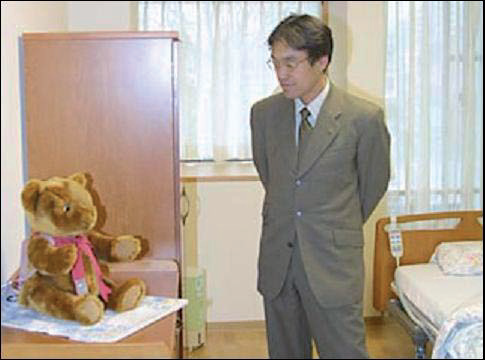
\includegraphics[scale=0.6]{fig/roboteddy}
 		\label{fig:roboTeddy}}
 	\hfill
 	\subfigure[Roboterkatze zur Therapie Quelle: \citep{wagner2009tele}]{%
 		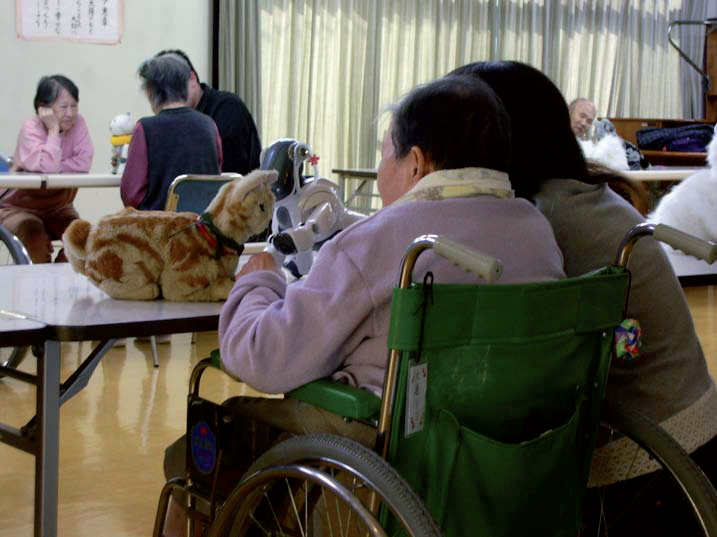
\includegraphics[scale=0.4]{fig/robocat}
 		\label{fig:roboTeddy2}}
 	\caption{Roboter in Seniorenheimen}
 	\label{fig:robSenioren}
 \end{figure}

Nicht nur in Japan, sondern auch in Deutschland wird sich mit dem Thema \textit{Care(rob)bots} befasst. So finden sich unter dem Stichpunkt \textit{Mensch-Maschine-Entgrenzungen} Studien zu der Thematik. Andere Untersuchungen befassen sich mit der Gegenseite, der Akzeptanz der Senioren\FemaleMale für Roboter. So ergab eine Befragung der VDE-Studie "Mein Freund der Roboter", dass eine Mehrheit (56\%) der Senioren\FemaleMale Robotern im Haushalt offen gegenüber stehen und diese einem Pflege-/Altersheim vorziehen würden. Neben den bekannten Staubsauger- und Rasenmährobotern, sind es auch zukünftige Anwendung, wie ein roboterisierter Rollstuhl, die hohe Akzeptanzwerte erreichen. Die Studie zeigte aber auch, dass Senioren\FemaleMale zunächst Robotern skeptisch gegenüberstehen. Spontan lehnten 40 Prozent der Senioren\FemaleMale Roboter in ihrem privaten Umfeld ab, 60 Prozent empfanden Robotik sogar als unheimlich. jedoch zeigte sich, dass der Wunsch nach einer selbstständigen Lebensführung ein starker Faktor für die Akzeptanz ist. Dadurch ergibt sich eine Beliebtheit für Serviceroboter. So sind Roboter, die abgrenzbare Tätigkeiten im Haushalt selbständig erledigen, sehr beliebt. Wichtige Kriterien für die Akzeptanz waren zudem die intuitive Bedienbarkeit, die Robustheit und die Flexibilität gegenüber unterschiedlicher Handicaps. Auch menschliche Faktoren wie Geduld, Verständnis, Höflichkeit und Achtung der Intimsphäre waren den Anwendern\FemaleMale wichtig.\citep{dr.sibyllemeyer2011}

Neben den sozialen Forschungen gibt es in Deutschland auch ingenieurwissenschaftliche Ergebnisse auf diesem Gebiet. So beschäftigt sich das  Cluster of Excellence Cognitive Interaction Technology (CITEC) in Bielefeld, zusammen mit der Stiftung Bethel, in der Forschung auf dem Gebiet der Unterstützung für Demenzkranke. Die dort entwickelten Assistenzsysteme helfen den Patienten unter anderem beim Zähneputzen und geben ihnen so ein Stück Selbstständigkeit zurück.

Viele Forschungen und Entwicklungen beschäftigen sich momentan mit der Mensch-Maschine/Roboter Beziehung. Dabei geraten die Roboter-Roboter-Interaktionen in den Hintergrund. Da aber heutige Roboter keine Allround-Lösungen bieten, sondern meist hochgradig spezialisiert sind und nur eine Tätigkeit ausführen können( zum Beispiel Saugroboter, Fensterwischroboter und weitere), ist das Zusammenspiel und die Komposition der Roboter wichtig. Das Szenario in Abbildung \ref{fig:szen1} zeigt, wie solch eine Komposition aussehen könnte.

\begin{figure}
	\centering
	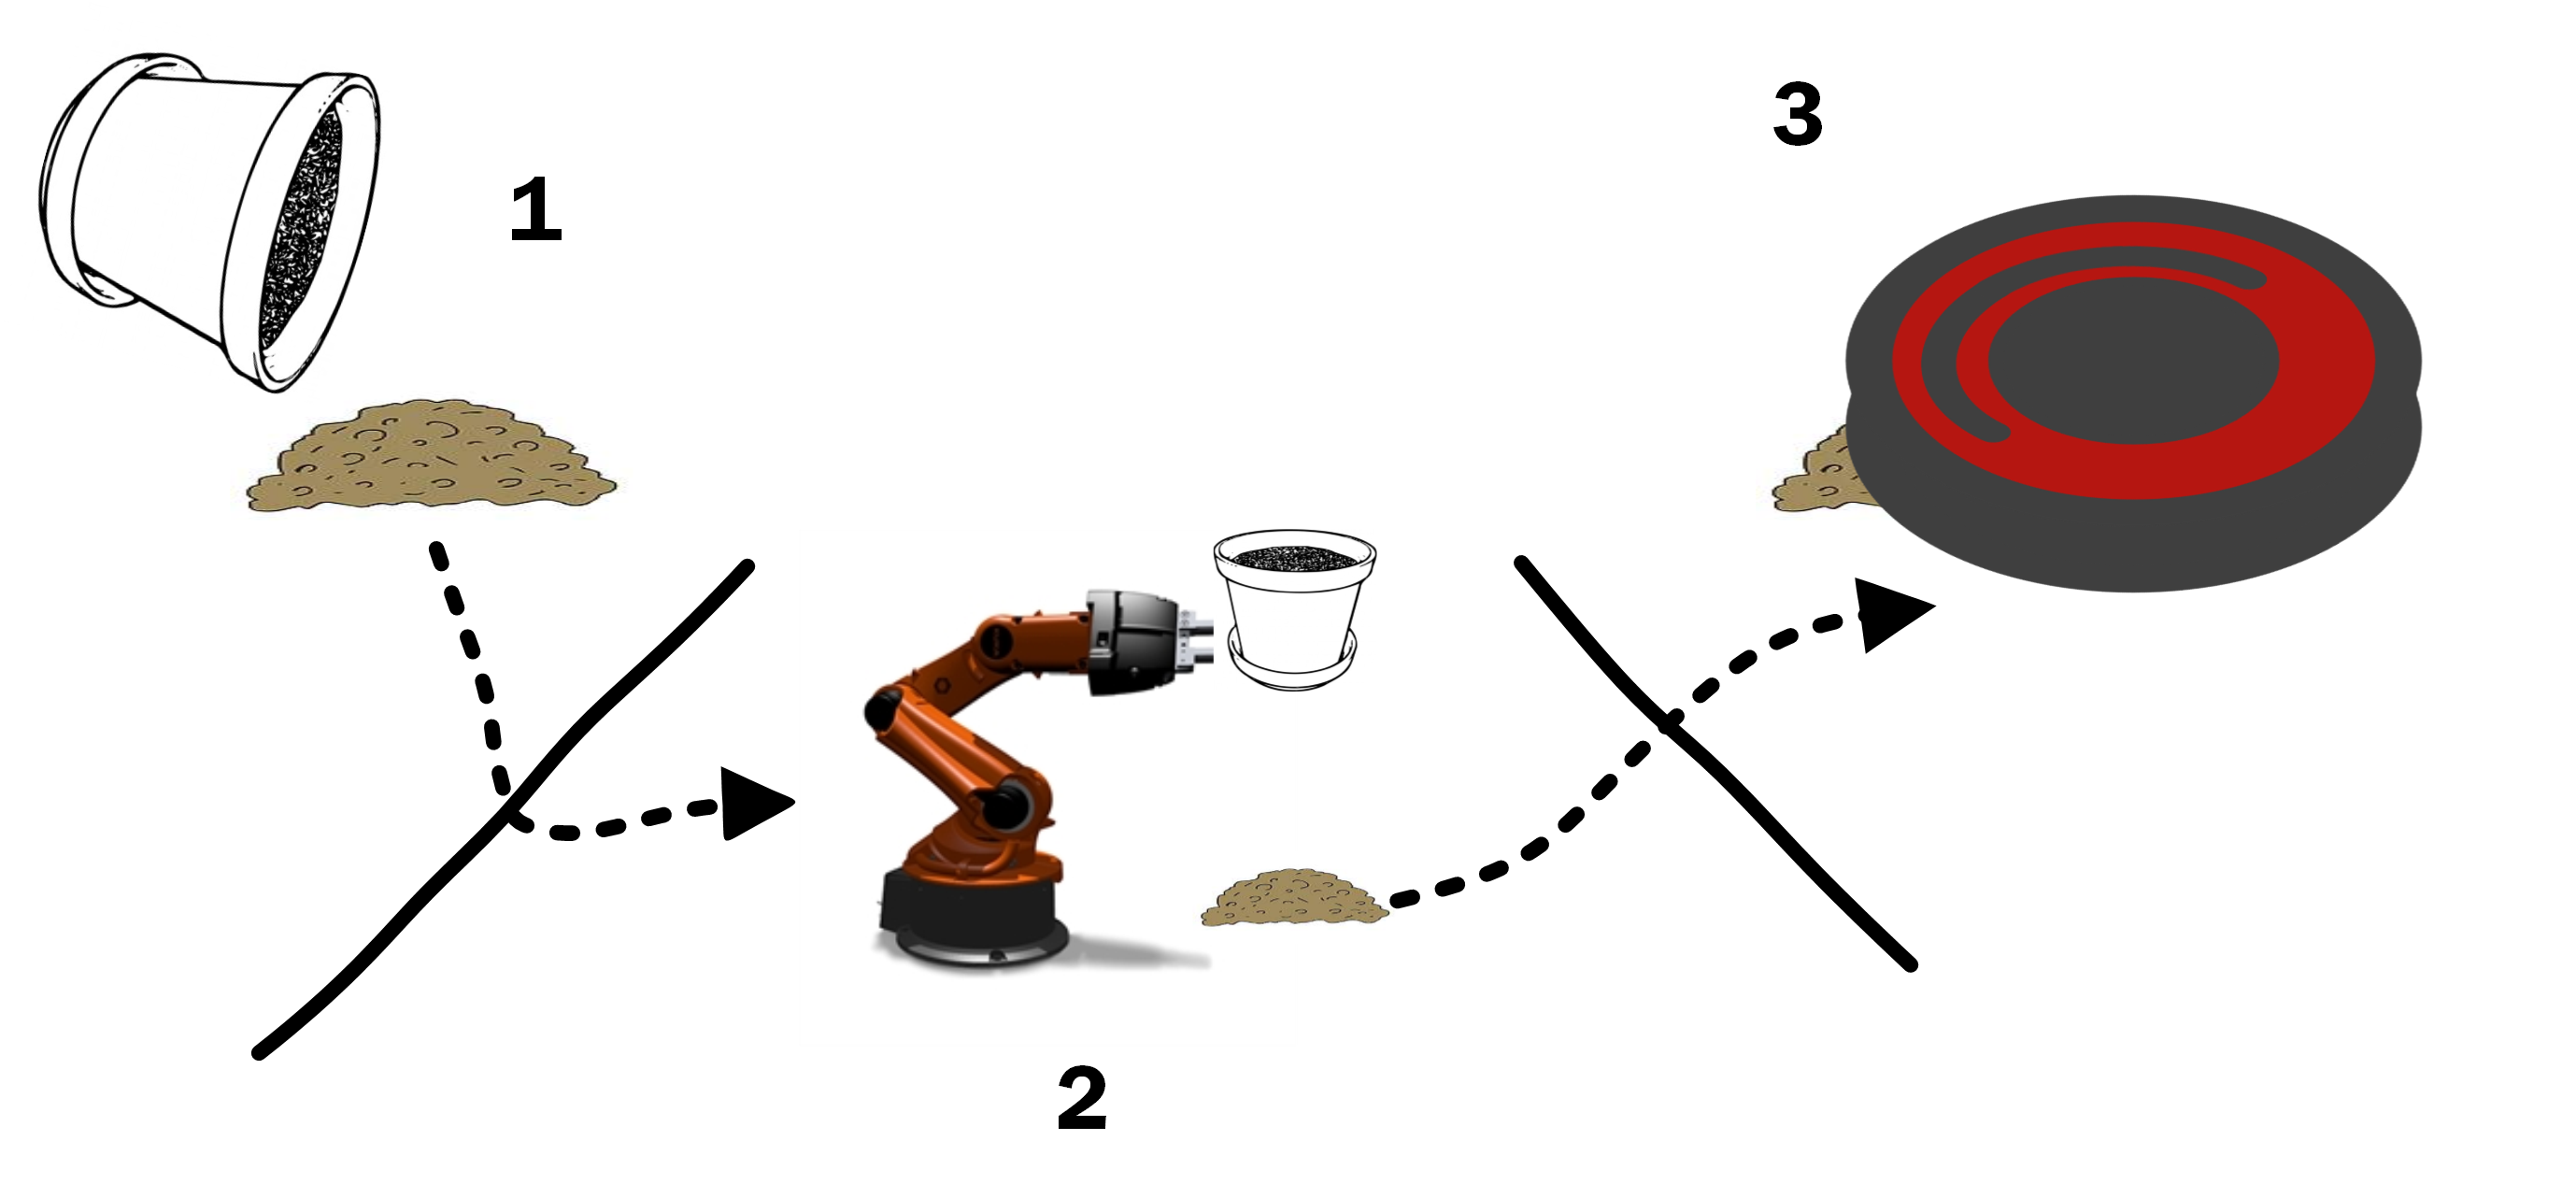
\includegraphics[scale=1.4]{fig/szen1}   
	\caption[Beispiel Szenario 1]{Mensch A stößt einen Blumentopf um (1). Ein Kamerasystem dediziert das der Topf umgefallen ist und Erde auf dem Boden liegt. Ein Roboter mit Arm wird gerufen, der zunächst die Vase aufhebt und an ihren Platz zurückstellt (2). Anschließend wird ein Saugroboter aktiviert, der die Erde weg saugt (3). Bei schwereren Verschmutzungen wird noch ein Wischroboter bestellt.}
	\label{fig:szen1}
\end{figure}

Dabei führt jeder Roboter selbstständig  und unabhängig von den anderen seine Arbeit aus. Die Kommunikation geht immer von der Zentralen Steuereinheit, dem \textit{Master}, aus. Zwischen den einzelnen Robotern findet kein großer Informationsaustausch statt. Die Änderung an dem Szenario in Abbildung \ref{fig:szen2} ändert jedoch die Art der Zusammenarbeit und der Kommunikation. Nun ist es nötig, dass die Roboter notwendige Informationen, wie die Übergabepose oder eine Synchronisierung der Gripper, austauschen.

\begin{figure}
	\centering
	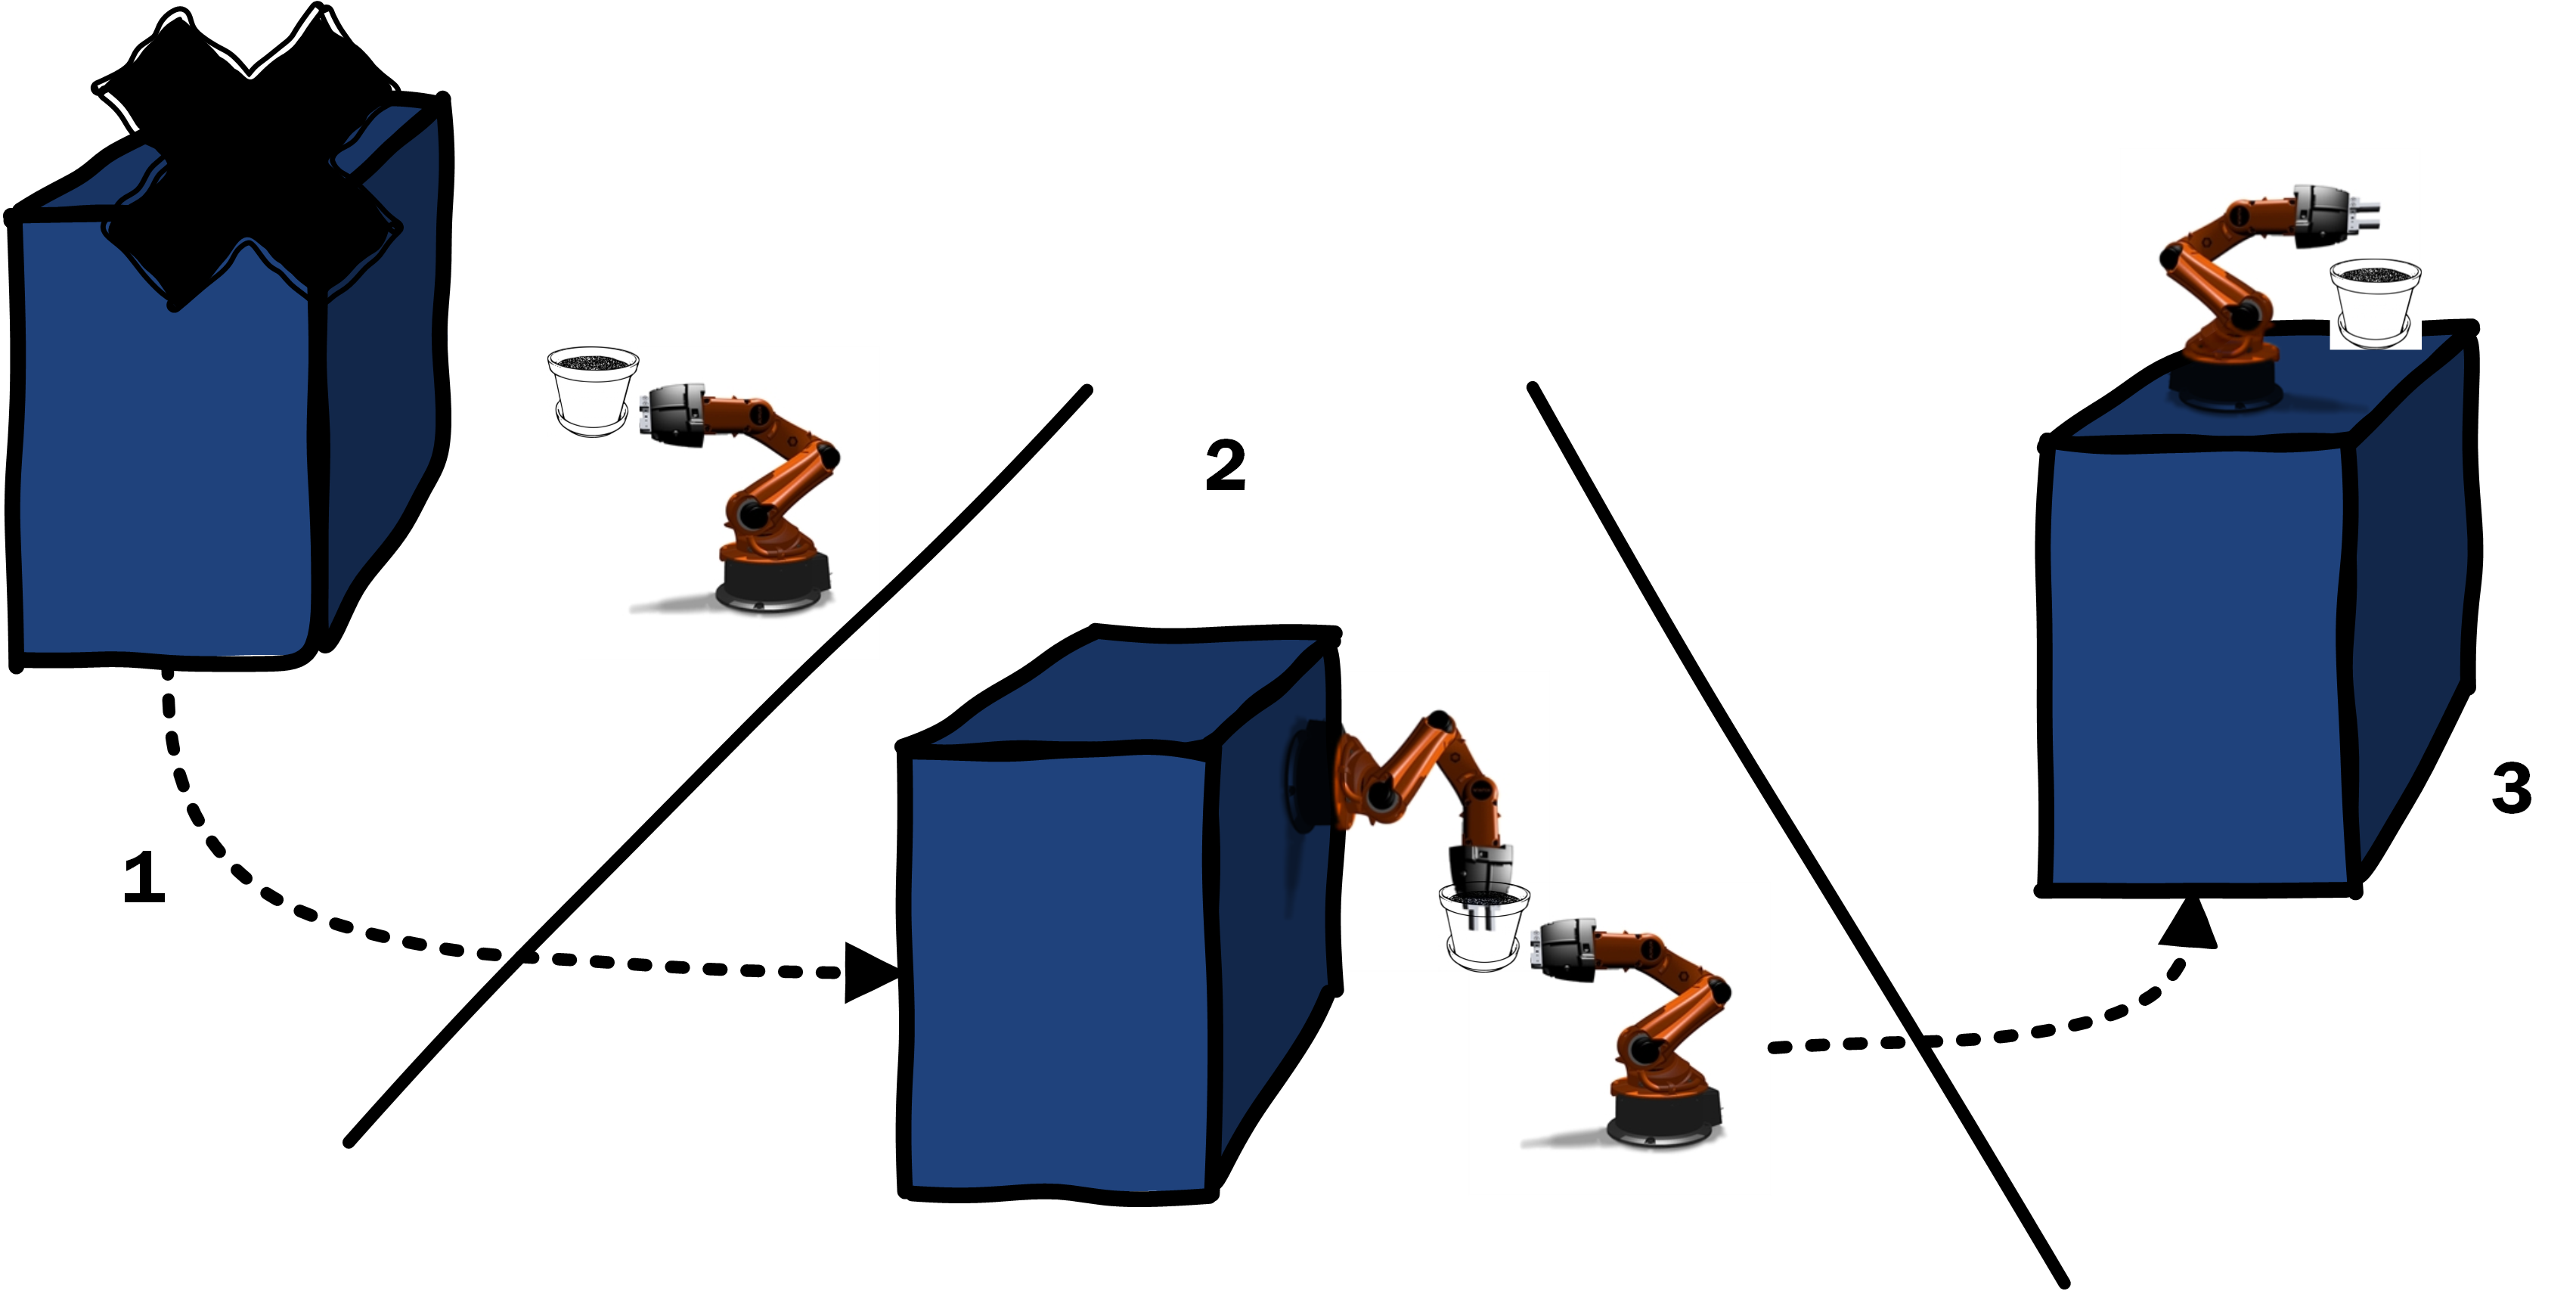
\includegraphics[scale=1.0]{fig/szen2}   
	\caption[Erweiterung Szenario 1]{Beim Zurückstellen der Vase stellt der Roboter fest, dass er die gewünschte Position nicht erreichen kann(1), weil sein Arm zu kurz ist. Da auf der Anrichte noch ein weiterer Arm steht nimmt er die Kommunikation mit diesem Manipulator auf. Sie kommunizieren einen Übergabepunkt und führen ein Übergabemanöver durch. Arm 2 stellt nun die Vase an die gewünschte Position.
	}
	\label{fig:szen2}
\end{figure}


Der zentrale Aspekt dieser Arbeit befasst sich mit dem Aufbau eines Multi-Robot-Systems, kurz MRS. Das Anwendungsszenario ist eine Abstraktion von Szenario 2. Roboter 1 übergibt ein Objekt an Roboter 2. Dabei werden verschiedene Thematiken der Robotik aufgegriffen, untersucht und erläutert. Kapitel \ref{sec:basics} befasst sich mit den Grundlagen auf denen diese Arbeit aufbaut. Neben der Nomenklatur wird die Middleware \textbf{R}obot \textbf{O}perating \textbf{S}ystem, kurz ROS, erläutert. Dabei wird auf den Aufbau, sowie die Kommunikationsschicht von Robotersystemen eingegangen. Anschließend folgt eine kurze Einführung in die mechanischen Grundlagen. Dabei werden die Begriffe rund um die Kinematik erklärt. 

In Kapitel \ref{sec:relatedwork} folgt eine detaillierte Übersicht der zugehörigen Literatur. Zunächst werden Arbeiten um das Thema MRS untersucht. Zentraler Aspekt dieser Thematik ist die Koordinierung von mehreren Robotersystemen. Drauf aufbauend wird das PEIS-Konzept erläutert. In diesem wird eine Nutzung von externen Sensoren für MRS gezeigt. Abschließend wird ein kurzer Einblick in Arbeiten zum Thema Greifen und Übergeben gegeben.

Das anschließende Kapitel \ref{sec:basic-aufbau} beschreibt den Aufbau des Teststandes, sowie die verwendete Hardware. Dabei wird auf die einzelne Sensoren und Aktoren eingegangen. Außerdem werden verschiedene Tests mit Prototypen durchgeführt, um die Genauigkeit und Qualität der Ergebnisse einzuschätzen.

Im Kapitel \ref{sec:entwicklung} werden die zentralen Aspekte dieser Arbeit beschrieben. Nach einer Auflistung von Nicht-Funktionalen Anforderungen, die bei der Entwicklung des MRS berücksichtigt werden sollen, werden einzelne Funktionalitäten des MRS entwickelt. Dabei werden Konzepte und Methoden vorgestellt. Anschließend folgt die Vorstellung der einzelnen Agenten, die für das Szenario benötigt werden. Diesen werden die Funktionalitäten und die Hardware zugewiesen. Diese Agenten werden durch das RATS miteinander verbunden. Diese Architektur bildet eine Schlüsselkomponente dieser Arbeit ab. Aufgabe von RATS ist die Zuweisung und Koordinierung von Aufgaben für unabhängigen Agenten. Diese Agenten können Sensoren, Aktoren oder Roboter sein. Anschließend wird die Entwicklung und Umsetzung einer geometrischen inversen Kinematik beschrieben. Diese ist für eine präzise Steuerung des Arms wichtig. Folgend wird in Kapitel \ref{sec:impl} die Umsetzung der Konzepte aus dem vorherigen Kapitel erläutert. Dazu werden die Algorithmen für verschiedene Funktionalitäten kurz dargestellt. Dabei werden Verfahren der Computer Vision und der Robotik angewandt. 

Zum Ende der Arbeit wird zunächst das entwickelte System in Kapitel \ref{sec:test} getestet und die Ergebnisse bewertet. Dabei wird sowohl auf funktionale, wie auch nicht-funktionale Anforderungen, eingegangen. Außerdem werden Problemstellen gesucht und analysiert, damit in Kapitel \ref{sec:end} im Ausblick Verbesserungsmaßnahmen vorgestellt werden können. Zuvor erfolgt jedoch eine Zusammenfassung der Arbeit. In dieser wird auf die Ergebnisse der Arbeit zurückgeblickt.



\clearpage


%%%%%%%%%%%%%%%%%%%%%%%%%%%%%%%%%%%%%%%%%%%%%%%%%%%%%%%%%%%%%%%%%%%%%%%
%% Grundlagen
%%%%%%%%%%%%%%%%%%%%%%%%%%%%%%%%%%%%%%%%%%%%%%%%%%%%%%%%%%%%%%%%%%%%%%%
%% Related Work
\section{Grundlagen}
\label{sec:basics}

Dieses Kapitel befasst sich mit den Grundlagen für die folgenden Kapitel. Es soll dem geneigten Leser Informationen zum Verständnis der Arbeit geben. Die anschließenden Unterkapitel beschreiben zunächst die verwendeten Mathematischen Ausdrücke und Bezeichner um die Lesbarkeit der späteren Formeln zu erleichtern. Nachfolgend wird die Middleware ROS genauer erläutert und unterschiedliche Funktionen sowie Einschränkungen aufgezeigt, die Auswirkungen auf die entwickelte Softwarearchitektur hatten. Darauf folgt eine Definition des Begriffs der Kinematik, welcher im späteren Verlauf der Arbeit für die Entwicklung der inversen Kinematik benötigt wird. Das abschließende Unterkapitel beschreibt die verwendete Hardware und den Laboraufbau im Detail. Weitere Informationen bezüglich der Robotik und grundlegender Mathematischer Begriffe sind im Buch "Robotics, Vision and Control" von Peter Corke zu entnehmen.

%%%%%%%%%%%%%%%%%%%%%%%%%%%%%%%%%%%%%%%%%%%%%%%%%%%%%%%%%%%%%%%%%%%%%%%
%% Related Work
\subsection{Nomenklatur}
\label{sec:basic-math}
    
  Die folgende Tabelle erläutert die genutzten mathematischen Symbole und orientiert sich an dem Buch \cite{Corke2011}. Von links nach rechts sind das Symbol, die Einheit und die Beschreibung gegeben. Einige Symbole werden mehrfach verwendet und haben je nach Kontext eine andere Bedeutung. Vektoren werden mit einem Bezeichner in \textbf{fett} gekennzeichnet.

  \begin{table}[h]%
  \begin{tabularx}{\columnwidth}{|l|l|X|}
  	\hline Symbol & Einheit & Beschreibung \\ 
  	\hline $T$ & s & Messintervall \\
 	\hline $T$ &  & homogene Transformation, $T \in SE(2)$ oder $SE(3)$ \\
 	\hline $^AT_B$ &  & homogene Transformation zur Darstellung von Koordinatensystem $ B $ betrachtet von Koordinatensystem $ A $. Koordinatensystem $ 0 $ bezeichnet das Weltkoordinatensystem und muss nicht explizit angegeben werden $^0T_B = T_B$(). Die inverse kann auf zwei Arten betrachtet werden: $(^AT_B)^{-1} = ^BT_A $ \\
 	\hline $\theta$ & rad & Winkel im Bogenmaß. Wenn nichts weiteres gegeben ist sind Winkel immer im \textbf{Bogenmaß} zu sehen. \\ 
 	\hline $ \pmb{\theta}$ & rad & Vektor von Winkel im Bogenmaß. \\ 
	\hline $\theta_r \theta_p \theta_y$ & rad & Roll-Pitch-Gear Winkel, beziehungsweise Rollen \\
 	\hline $\alpha$ & \textdegree & Winkel in Grad. Wenn nichts weiteres gegeben ist sind Winkel immer im \textbf{Bogenmaß} zu sehen. \\
 	\hline $v$ & m s$^{-1}$ & Geschwindigkeit. \\
 	\hline $\pmb{v}$ &  m s$^{-1}$  & Geschwindigkeitsvektor. Meist $\in \mathds{R}^3$. \\
 	\hline $\omega$ & rad s$^{-1}$ & Drehwinkel-Geschwindigkeit. \\
 	\hline $\pmb{\omega}$ &  rad s$^{-1}$  & Drehwinkel-Geschwindigkeitsvektor. Meist $\in \mathds{R}^3$. \\
 	\hline $\pmb{v}$ &  & Geschwindigkeit-Drehung (engl. Twist, Screw).  $\pmb{v} \in \mathds{R}^6$, $\pmb{v} = (v_x, v_y, v_z,\omega_x, \omega_y, \omega_z)$ \\
 	\hline X,Y,Z &   & Kartesische Koordinaten. \\
 	\hline $\xi$ &   & Abstrakte Darstellung einer 3-dimensionalen Kartesischen Pose  $\xi  \in \mathds{R}^6$ \\
 	\hline $^A\xi_B$ &   & Abstrakte Darstellung einer \textbf{relativen} 3-dimensionalen Kartesischen Pose, Pose $ B $ betrachtet von Pose $ A $ \\
	\hline $\oplus$ &   & Hintereinanderausführung (Addition) zweier Posen \\
	\hline $\ominus$ &   & Unärer Operator zur Invertierung von Posen \\
 	\hline
  \end{tabularx}
  \caption{Nomenklatur}
  \label{tab:nomenklatur}
  
    \end{table}%
  


%%%%%%%%%%%%%%%%%%%%%%%%%%%%%%%%%%%%%%%%%%%%%%%%%%%%%%%%%%%%%%%%%%%%%%%
%% Related Work
\subsection{ROS: Robotic Operating System}
\label{sec:basic-ros}
    
Das Robotic Operating System, kurz ROS, ist ein Middleware-Framework zur Steuerung und Verwaltung von Personal-Robotern. Es verwendet eine Paket und Node Struktur um einzelne Aktoren und Sensoren einzelner Robotersystem zu betreiben. Das ROS dient dabei als Abstraktionsebene für die Entwickler und versucht die Anwendungsebene von der Hardwareebene zu trennen. Das Framework wird am Robotikinstitut Willow Garage in Zusammenarbeit mit der Open Source Robotics Foundation entwickelt, stammt aber ursprünglich vom Stanford Artificial Intelligence Laboratory. Dort wurde 2007 im Rahmen des Stanford-AI-Robot-Projektes die Entwicklung aufgenommen. ROS ermöglicht während der Entwicklung und des Betriebs ein Cross-Plattform System, da es kompatible Versionen für Windows (experimentell), Linux und Mac OS X gibt. Außerdem steht ein Multi(programmier)sprachen System zur Verfügung. So ist es möglich, eigene Nodes mit C++, Python oder Java zu entwickeln \citep{quigley2009ros}. Neben den Standardkonzepten und -paketen gibt es eine Community, die eigene Pakete auf der ROS-Homepage zur Verfügung stellt. Die folgenden Abschnitte erläutern die ROS-Kernkonzepte, welche für die Entwicklung eingesetzt wurden. Als Grundlage für das komplette Kapitel wurde die Dokumentation von ROS genutzt.

\subsubsection{Packages und Nodes}

\textit{Packages} dienen der strukturellen Verwaltung aller Dateien im ROS-System. Nodes, Launch-Files, Services, Actions und Messages (siehe unten) sind immer an ihr Paket gebunden und können nur unter deren Namen erreicht werden. Für die Verlinkung und die Erreichbarkeit gebauter Pakete ist das ROS-interne Buildsystem \textit{Catkin} zuständig. Es benötigt ebenfalls den \textbf{eindeutigen} Package-Namen für den Build und Verwaltungsprozess. Neben den ROS-bezogenen Daten können in einem Paket aber auch ROS unabhängige APIs angelegt und verwaltet werden. So werden unter anderem einzelne Pakete für Treiber genutzt. Ein ROS-Paket folgt dem Goldilocks-Prinzip: Genug Funktionalität um nützlich zu sein, aber nicht zu viel, damit die Verwendbarkeit nicht zu komplex wird \citep{roswiki}.

Neben der strukturellen Verteilung gibt es auch die funktionale Trennung. Diese wird durch einzelne \textit{Nodes} erreicht. Jeder Node hat einen bestimmten Aufgabenbereich. Erst das Zusammenspiel mehrerer Nodes ergibt ein Robotersystem. So ist ein Node zum Beispiel für die Berechnung der inversen Kinematik zuständig, ein anderer für die Lokalisierung des Roboters im Raum und ein dritter für das User-Interface. Diese Verteilung der Funktionalitäten hat mehrere Vorteile. Da jeder Node in einem eigenen Prozess gestartet wird, ist das komplette System robuster. Jeder Node muss so entwickelt werden, dass er eigenständig weiterlaufen kann, auch wenn ein benötigter Node durch einen Fehler abgestürzt ist. Jeder Node wird mit einem systemweit einmaligen Namen aufgerufen unter dem er vom System erreicht und angezeigt werden kann. Nodes kommunizieren untereinander mit Hilfe von Topics (siehe \ref{sec:basic-ros-topics}). Soll ein ROS Node gestartet werden kann dieser mit Hilfe des ROS-Befehls aufgerufen werden \citep{roswiki}:

\begin{lstlisting}[language=bash]
rosrun <paket-name> <nodetype-name>
\end{lstlisting}

Der Paketname und der Nodetype sind erforderliche Felder. Darüber hinaus können Parameter angegeben werden, die für den Node notwendig sind. Eine weitere Möglichkeit einen und mehrere Nodes zu starten, ist ein Launchfile. In diesem können Nodes, Parameter und Argumente aufgelistet werden. Zu beachten ist jedoch, dass die Nodes in einer zufälligen Reihenfolge gestartet werden. Ein Launch-File kann mit folgendem Befehl gestartet werden \citep{roswiki}:

\begin{lstlisting}[language=bash]
roslaunch <paket-name> <launchfile-name>
\end{lstlisting}

Damit ein Node gestartet werden kann, muss vorher ein ROS-Master aktiv sein, mit dem sich der Node verbinden kann. Ist der Node verbunden kann er auf die Topics, Services, Actions und den Parameter-Server des Master zugreifen \citep{roswiki}.

\subsubsection{Master und Parameter-Server}
Der ROS Master ist ein zentraler Dienst für ganze System. Er beinhaltet einen Namen- und Registrierungs-Service an dem sich andere Nodes, auch Services, anmelden können. Der Master wird benötigt, damit die Nodes sich gegenseitig im System verbinden können. Der Nachrichten-Transport geht nicht direkt über den Master. Dieser verbindet nur die beiden Nodes, welche anschließend via einer Peer-to-Peer Verbindung kommunizieren \citep{roswiki}. In Abbildung \ref{fig:basic-ros-masternode} ist eine solche Verbindung dargestellt.

 \begin{figure}[h]
 	\centering
 	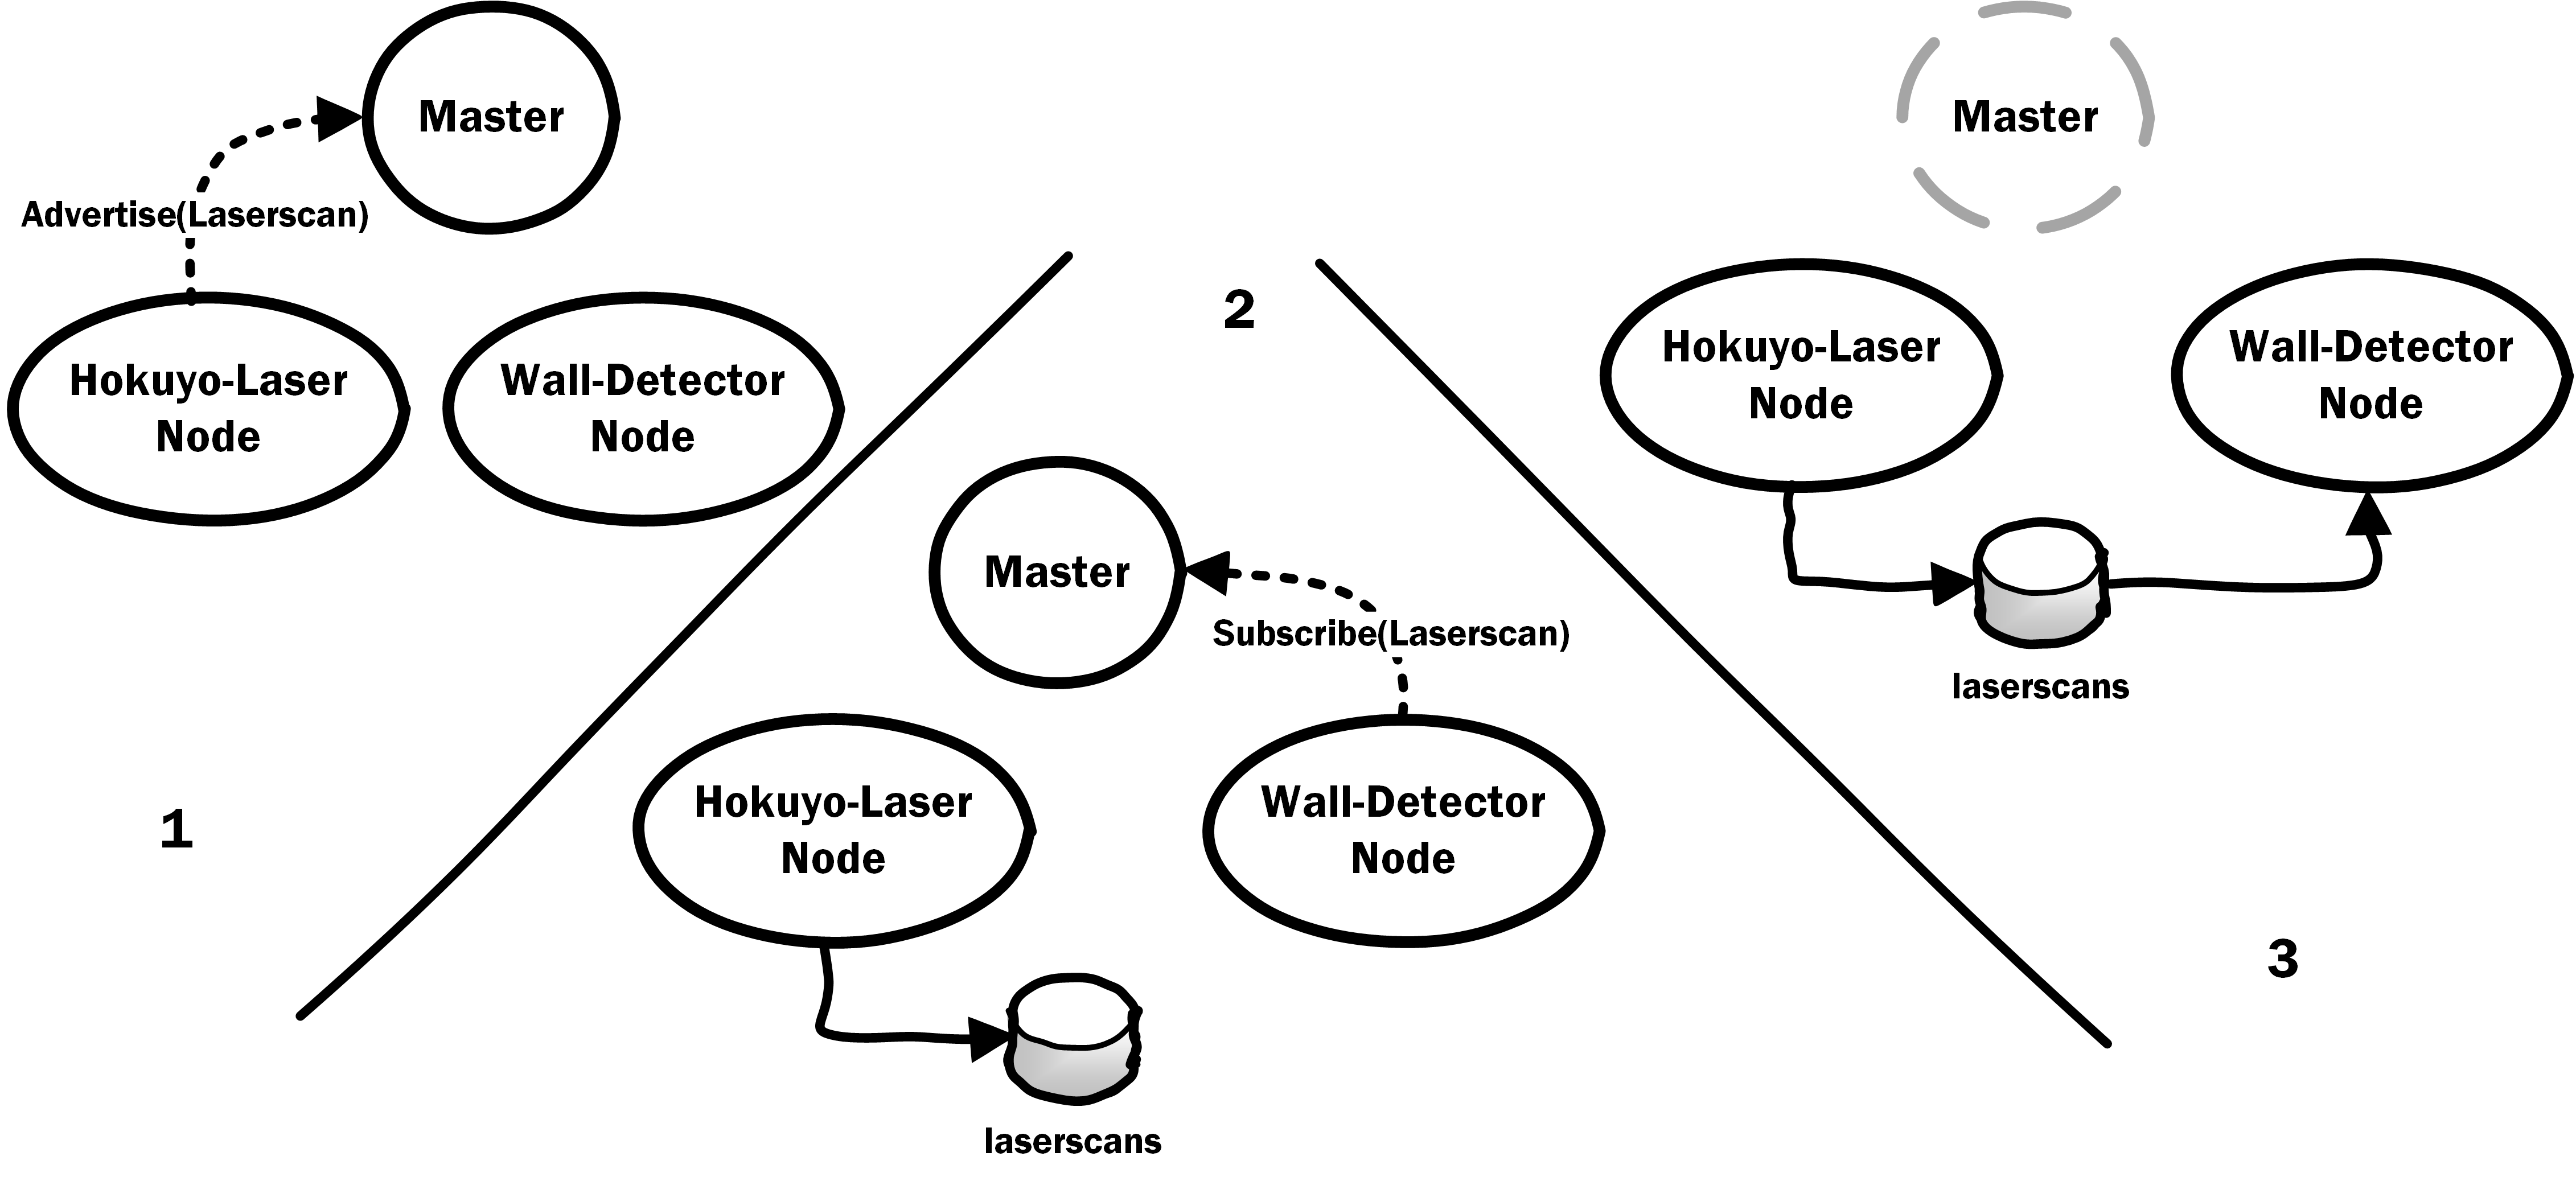
\includegraphics[scale=0.8]{fig/masternode}   
 	\caption[Master-Service]{Master-Service: (1) Der Hokuyo-Laser-Node meldet sich beim Master an, dass er Laserscans zur Verfügung stellt. (2) Der Laser-Node stellt seine Daten zur Verfügung und der Wall-Detector meldet sich beim Master, dass er Laserscans benötigt. Der Master stellt die Verbindungsinformationen bereit und zieht sich dann zurück (graue Markierung). (3) Die Verbindung zwischen Laser-Node und Detector-Node ist hergestellt.}
 	\label{fig:basic-ros-masternode}
 \end{figure}
 
 Dieses Verfahren reduziert die Netzwerklast stark im Vergleich zu einem Broadcasting-Verfahren. Eigene Tests im Rahmen dieser Arbeit zeigten, dass der Kamera-Node \textit{openni2} ein Netzwerk mit den berechneten 3D-Punktwolken vollständig auslastet. Dabei wurde die Punktwolke auf einer physikalischen Maschine  erzeugt und auf eine zweite Maschine via WLAN übertragen. Die Verzögerung der Wolken war dabei mit über fünf Sekunden im Schnitt sehr hoch und wurde höher, je länger die Übertragung dauerte. Eine Lösung (siehe \ref{fig:basic-ros-masternet}) bietet die Vorverarbeitung der Daten auf der Maschine. Dabei werden nur noch die gefilterten Daten übertragen, sowie die Übertragungsrate reduziert. Dadurch ist die Übertragung der Daten unkritisch. Nun gingen nur noch die Verbindungsdaten zwischen Nodes und Master und die reduzierte Datenmenge über das Netzwerk.
 
 \begin{figure}[h]
 	\centering
 	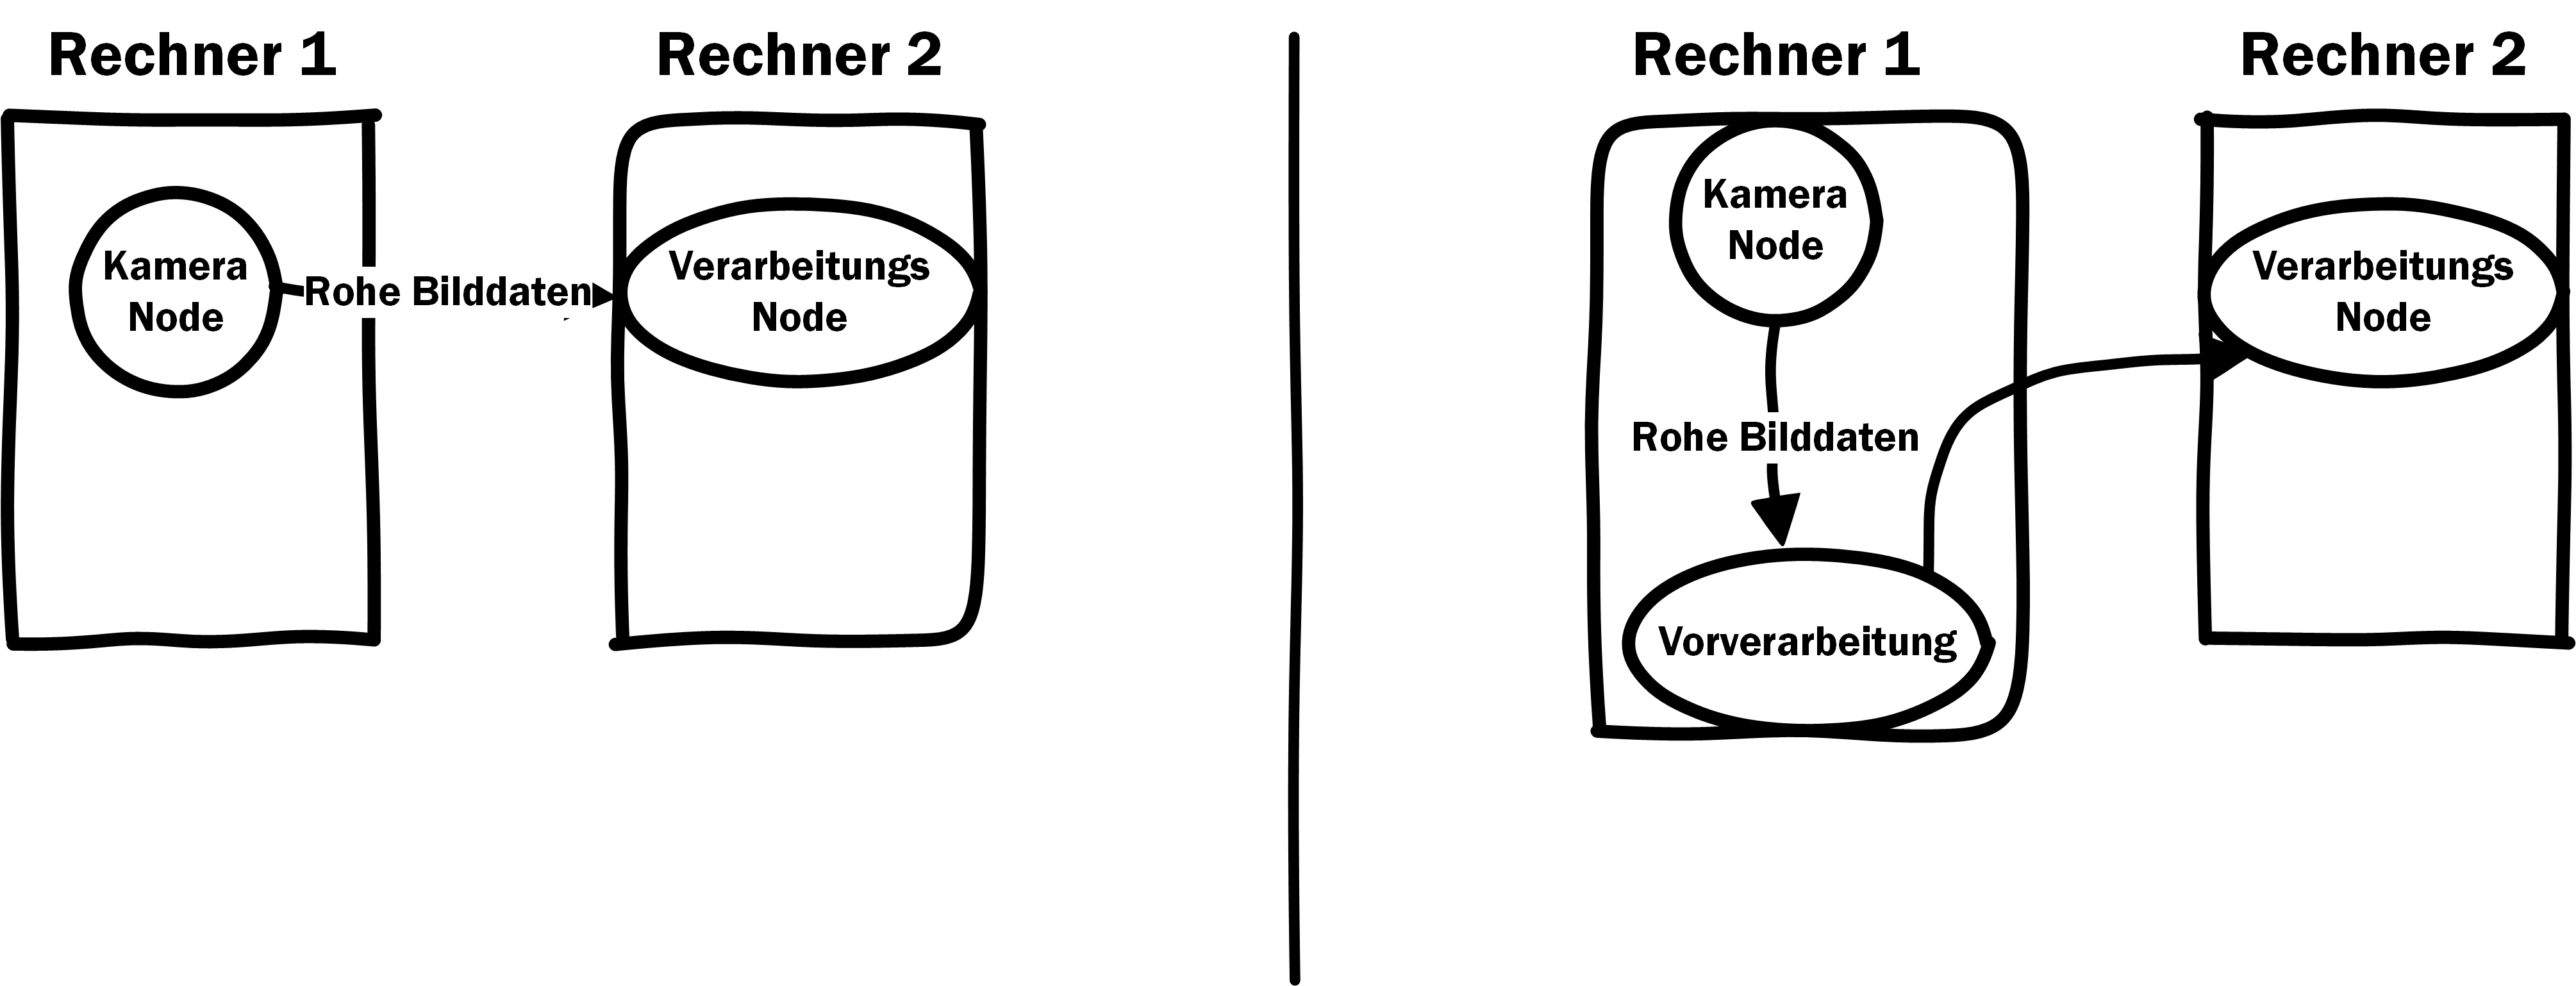
\includegraphics[scale=0.8]{fig/masternet}   
 	\caption[Netzwerk Entlastung durch Peer-to-Peer Verbindungen]{Netzwerk Entlastung durch Peer-to-Peer Verbindungen. Links: ohne Datenvorverarbeitung, Rechts: mit Datenvorverarbeitung.}
 	\label{fig:basic-ros-masternet}
 \end{figure}
 
 Neben dem Namens-Service verwaltet der ROS-Master auch den Parameter-Server. Dieser besteht aus einer großen Key-Value-Map, dem Wörterbuch. Dieses kann global erreicht werden. Nodes haben so die Möglichkeit, vordefinierte Daten zu lesen oder selber welche zu schreiben. So können Sensoren oder Aktoren kalibriert und konfiguriert werden. Der Zugriff auf diese Daten hat keine hohe Performance. Er ist für einen statischen Zugriff gedacht und kann mit einer Baum-Struktur geordnet werden, so lassen sich zusammenhängende Daten mit einer Abfrage am Server abrufen \citep{roswiki}.

\subsubsection{Topics und Messages}
\label{sec:basic-ros-topics}

ROS bietet für die Kommunikation zwischen Nodes ein \textit{Topic}-System. Jeder Topic entspricht dabei einem benannten Bus, auf welchen anonyme \textit{Publisher} und \textit{Subscriber} zugreifen können. Die Daten können dabei als TCP-Pakete (TCPROS) oder als UDP-Pakete (UDPROS) gesendet werden. Ein Topic besitzt einen eindeutigen Namen im System und einen eindeutigen Typen, der anhand des übersendeten Message-Typen definiert wird. Jede Topic kann nur einen Message-Typen versenden. Dieser Type ist nicht im Master bekannt, jedoch können sich Subscriber nur mit dem entsprechenden Typen anbinden. Die Anzahl der Subscriber und Publisher für einen Topic ist nur durch die Systemleistung beschränkt \citep{roswiki}. In Abbildung \ref{fig:basic-ros-topic} ist ein solcher Topic dargestellt.

\begin{figure}[h]
	\centering
	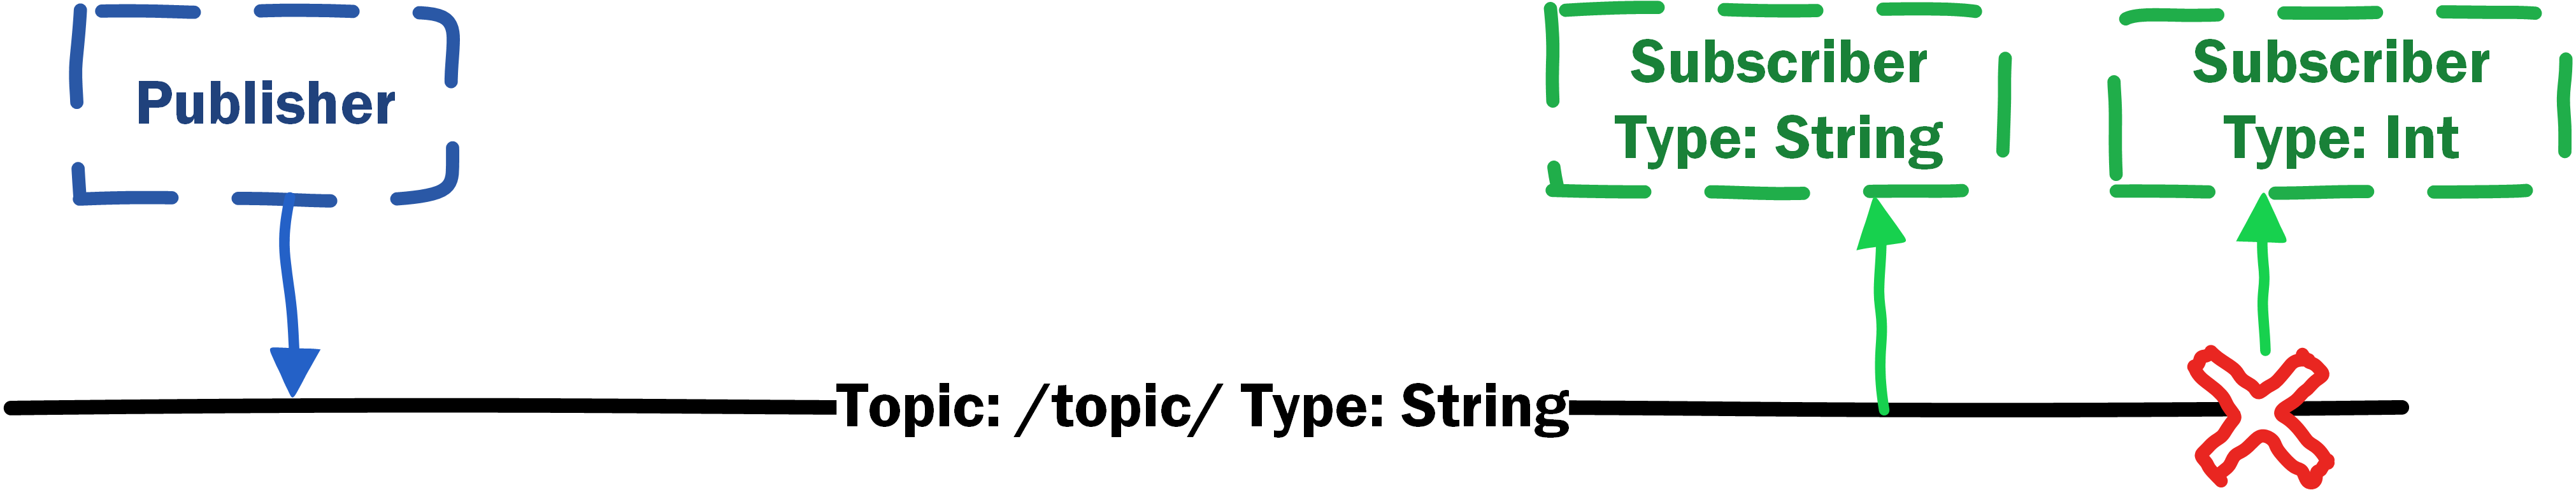
\includegraphics[scale=0.8]{fig/topic}   
	\caption[Topic Beispiel]{Beispiel für ein Topic mit dem Namen /topic/ und dem Type String. Ein Publisher schreibt Daten in den Bus, ein Subscriber liest diese aus. Die Verbindung eines zweiten Subscribers schlägt auf Grund des falschen Types fehl.}
	\label{fig:basic-ros-topic}
\end{figure}

Publisher veröffentlichen ihre Daten in den Bus und haben nur einen schreibenden Zugriff. Sie bekommen kein Feedback, an wen die Daten gesendet worden sind, oder ob die Daten überhaupt empfangen worden sind. Der erste Publisher, der sich auf einem Topic verbindet, gibt den Typen vor \citep{roswiki}.

Subscriber lesen die Daten vom Bus und geben sie für die Weiterverarbeitung weiter. Sie bekommen normalerweise keine Informationen über den Absender der Daten. Subscriber können sich nur bei einem Topic registrieren, wenn der Message-Type stimmt \citep{roswiki}.

Subscriber und Publisher haben jeweils eigene Cache-Systeme, die Nachrichten vor- oder zurückhalten können. Ein Topic ist ein einfachgerichteter Streaming-Dienst. Da in einem Roboter-System auch Remote-Procedure-Calls benötigt werden, um zum Beispiel Antworten auf Anfragen zu erhalten oder synchronisierte Aufgaben zu erledigen, wurde das Service-Paket als weiteres Kernkonzept angelegt \citep{roswiki}.

\subsubsection{Services}

\textit{Services} ermöglichen es einen Remote-Procedure-Call Node-übergreifend durchzuführen. Dazu muss Node A seinen Service am Master registriert haben und einen Service-Server gestartet haben. Node B kann nun mit einem Service-Client auf den registrierten Service zugreifen und eine Anfrage starten. Während die Anfrage verarbeitet wird, kann Node B nun je nach Anforderung blockieren oder weiter arbeiten. Node A verarbeitet nun die Anfrage und antwortet Node B mit dem Ergebnis. Der Service selbst, sowie die Parameter und die Rückgabewerte, sind für jeden Service eindeutig und werden vorher über zwei Messages, eine für die Request und eine für die Response, festgelegt. Analog zu den Topics werden Services am Master mit einem eindeutigen Namen angemeldet, unter dem sie erreichbar sind. Dies ermöglicht auch einen einfachen Austausch von verschiedenen Implementierungen \citep{roswiki}.

\subsubsection{Action-Lib}
\label{sec:basic-ros-action}
Ein aktiver Service schickt erst eine Rückmeldung an den Aufrufer, wenn er seine Aufgabe erledigt hat. Um auch einen Zwischenstand schicken zu können, wurde die Action-Lib eingeführt. Dieses Paket ist eigentlich keine Entwicklung der ROS-Entwickler sondern ein Community-Package. Inzwischen wurde es aber von der OSR-Foundation übernommen und als eins der Kernkonzepte eingestuft \citep{roswiki}.

Analog zu den Services besitzt auch die Action-Lib einen Server- und einen Client-Teil. Der Client fordert vom Server eine Aktion an, dabei übergibt er ein \textit{Goal}. Dieses beinhaltet die benötigten Parameter für den Server. Der Server arbeitet die Anfrage ab, dabei kann er auch \textit{Feedback} zurückschicken. Dies können mögliche Zwischenergebnisse oder Fortschrittsmarken sein. Ist die Anfrage abgearbeitet, schickt der Server ein \textit{Result} an den Client zurück. Wie auch beim Service ist die Art der Aktion eindeutig. Die Anzahl der Parameter bei Goal, Feedback und Result sind fest definiert und können zur Laufzeit nicht geändert werden \citep{roswiki}.
%%%%%%%%%%%%%%%%%%%%%%%%%%%%%%%%%%%%%%%%%%%%%%%%%%%%%%%%%%%%%%%%%%%%%%%
%% Related Work
\subsection{Kinematik }
\label{sec:basics-ik}
    
Dieses Unterkapitel befasst sich mit dem Begriff der Kinematik und den dazu gehörigen Begriffen des Mechanismus und der inversen Kinematik. Außerdem werden einige mathematische Lösungswege für verschiedene Probleme innerhalb der genannten Themen genannt.

\subsubsection{Mechanismus}

Ein Mechanismus ist der Grundbegriff von beweglichen Körper. Dabei wird zwischen \textit{Gliedern} (engl. Link, $L$ = Set of Links) und \textit{Gelenken} (engl. Joint, $J$ = Set of Joints) unterschieden. Glieder sind die starren Körper eines Mechanismus und sind durch Gelenke miteinander verbunden. Ein Glied ist nicht auf ein Gelenk beschränkt, sondern kann mehrere haben ($N_{joint} \in \mathds{N}_0$). Auch die Verbindung zwischen zwei Gliedern kann durch mehrere  Gelenke realisiert sein. Ein Gelenk wiederum ist auf genau zwei Glieder beschränkt  ($N_{link} = 2$) und ermöglicht so eine eingeschränkte relative Bewegung zueinander. Gelenke werden nicht als eigenständige physikalische Körper gesehen. Gelenkhälften, zum Beispiel die Schenkel eines Kippscharniers, werden als Bestandteil des damit verbundenen Gliedes betrachtet. Die folgenden Definitionen sind als Denavit–Hartenberg Parameter bekannt \citep{Corke2011}.

Glieder können mit zwei Parametern definiert werden, der Länge $a$ und der Verdrehung $\alpha$:

\begin{displaymath}
	l_i \in L \\
\end{displaymath}

\begin{equation}
a_i =  \text{Länge von } l_i
\end{equation}

\begin{equation}
\alpha_i =  \text{Verdrehung von } l_i 
\end{equation}

Gelenke werden ebenfalls mit zwei Parametern definiert. Der Gelenk-Offset beschreibt den Abstand zwischen den zwei Gliedern eines Gelenks auf der Gelenkachse. Der Gelenkwinkel beschreibt die Rotation zwischen den beiden verbundenen Glieder im Bezug zur Gelenkachse\citep{Corke2011}.  Zur Veranschaulichung dieser Nomenklatur ist die Abbildung \ref{fig:ik-dh} vorhanden. Dabei sind die Parameter in rot dargestellt. Außerdem werden die einzelnen Koordinatensysteme der Gelenke gezeigt.

\begin{displaymath}
j_i \in J \\
\end{displaymath}

\begin{equation}
d_i =  \text{Gelenk-Offset von } j_i
\end{equation}

\begin{equation}
\theta_i =  \text{Gelenkwinkel von } j_i 
\end{equation}

\begin{figure}[H]
	\centering
	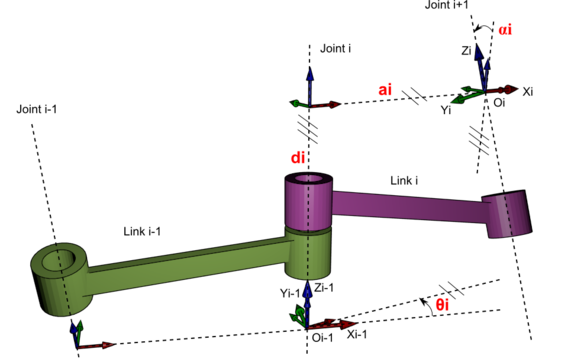
\includegraphics[width=0.8\textwidth]{fig/dh}   
	\caption[Darstellung Denavit–Hartenberg Parameter]{Darstellung Denavit–Hartenberg Parameter. Bildquelle \cite{wiki}}
	\label{fig:ik-dh}
\end{figure}

\subsubsection{Kinematik}
\label{sec:basics-ik-k}

Die \textit{Kinematik} eines Mechanismus beschreibt die Bewegungsmöglichkeiten der Glieder relativ zueinander. Es wird dabei abstrahiert, ob ein Gelenk motorisch angetrieben oder passiv bewegt wird. Die Kinematik betrachtet bei der Bewegung auftretende \textit{Geschwindigkeiten} und \textit{Beschleunigungen}. Auftretende Kräfte werden nicht in der Kinematik, sondern in der \textit{Dynamik} untersucht. Zentrale Aspekte dabei sind die Trägheits- und Schwerkraft.

Die \textit{Kinematische Kette} beschreibt den Aufbau eines speziellen Mechanismus. Dabei ist die Anzahl der Gelenke pro Glied auf maximal 2 beschränkt ($N_{joint} <= 2$). Besitzt jedes Glied genau zwei Gelenke gilt die Kette als geschlossen, ansonsten als offen.

\begin{equation}
	 \text{Kinematische Kette} = 
	\begin{cases}
		geschlossen & \forall l \in L | l_{joints} = 2 \\
		offen & \text{für Rest} \\
	\end{cases}
\end{equation}

Für diese Arbeit ist nur die offene Kette interessant, da die Manipulatoren der meisten Roboter an beiden Enden (Base und End-Effektor) frei sind. Dadurch ergibt sich für $N_{link} = N_{joint} + 1$. Typischerweise wird das erste Gelenk mit dem Index 1 versehen und das erste Glied mit dem Index 0. Glied 0 ist die \textit{Base} des Manipulators und Glied N beinhaltet den\textit{ End-Effektor}. Aus der Bezeichnung ergibt sich, dass Gelenk j die Glieder j-1 und j mit einander verbindet und das Glied j bewegt \citep{Corke2011}. 

Die Transformation eines Glied-Koordinatensystems {j-1} zu Glied {j} wird durch elementare Rotation und Translation beschrieben (siehe auch Abbildung \ref{fig:ik-dh}):

\begin{equation}
^{j-1}A_{j}(\theta_j,d_j,a_j,\alpha_j) = T_{Rz}(\theta_j)T_{z}(d_j)T_{x}(a_j)T_{Rx}(\alpha_j)
\label{f:basics-ik-k}
\end{equation}


Durch die Vereinigung der einzelnen Matrizen ergibt sich \cite{Corke2011}:
\begin{equation}
^{j-1}A_{j}(\theta_j,d_j,a_j,\alpha_j) = 
\begin{pmatrix}
cos \theta_j & -sin \theta_j cos \alpha_j & sin \theta_j sin \alpha_j  & a_j cos \theta_j\\
sin \theta_j & cos \theta_j cos \alpha_j & -cos \theta_j sin \alpha_j  & a_j sin\theta_j\\
0 			&sin \alpha_j 				& cos \alpha_j  & d_j\\
0 & 0 & 0& 1\\
\end{pmatrix}
\end{equation}

\subsubsection{Forward Kinematics}

Die Vorwärts-Kinematik (engl. Forward Kinematic) beschreibt die "vorwärts"  Rechnung der Kinematik. Aus den gegebenen Gelenk-Informationen wird die Pose des End-Effectors $\xi_E$ berechnet. Hier reichen die Daten für den Gelenkwinkel $\theta_j$ bei Drehgelenken und für den Winkel-Offset $d_j$ bei Schiebe-/ Schubgelenken, da die restlichen Werte für den Mechanismus als konstant angesehen werden können. Die Forward Kinematic wird häufig als Funktion $K$ angegeben \citep{Corke2011}.

\begin{equation}
\xi_E = K(\textbf{q})
\label{f1}
\end{equation}

$q$ entspricht dabei der aktuellen Gelenk-Konfiguration und $\xi_E$ der Pose des End-Effectors. Durch die Kombination der Transformation aus Gleichung \ref{f:basics-ik-k} ergibt sich für einen Manipulator mit N-Gelenken  \cite{Corke2011}. Dies wird benötigt, um die aktuelle Pose des End-Effektors für den Roboter zu berechnen. In dem Anwendungsszenario für diese Arbeit wird dies unter anderem für Positionsüberprüfungen und Kollisionskontrollen, aber auch für die Übergabe benötigt.

\begin{equation}
\xi_E \sim \: ^0T_E =\: ^0A_1\:^1A_2 \:\dots\:^{N-1}A_N
\end{equation}

\subsubsection{Inverse Kinematik}

Die Inverse Kinematik berechnet die Inverse der Forward-Kinematic. Sie bestimmt die möglichen Gelenk-Konfigurationen $\textbf{q}$ für eine Zielpose. Im Gegensatz zur Forward-Kinematic ist die Inverse Kinematik nicht eindeutig. Eine einfache Veranschaulichung kann man am menschlichen Körper sehen. Fixiert man das Handgelenk an einer Position kann man den Ellenbogen in verschiedene Positionen bewegen, ohne die Position der Schulter zu ändern. Für die Inverse Kinematik ergibt sich folgende Funktion für eine beliebige Pose $\xi$ \citep{Corke2011}:


\begin{equation}
\textbf{q} = K^{-1}(\xi)
\label{f2}
\end{equation}

Aus Gleichung \ref{f1} und \ref{f2} ergibt sich auf Grund der Eindeutigkeit:

\begin{displaymath}
\xi = K(K^{-1}(\xi))
\end{displaymath}

Aber \textbf{nicht}
\begin{displaymath}
\textbf{q} = K^{-1}(K(\textbf{q}))
\end{displaymath}

Um eine Inverse Kinematik zu lösen gibt es drei Methoden: geometrisch (analytisch), numerisch und heuristisch \citep{danielasteidl2011}.

Die geometrische Lösung nutzt die einfache geometrische Abstraktion des Mechanismus und versucht diesen mit trigonometrischen Funktionen abzubilden. Damit auch hier mehrere Lösungen bestimmt werden können, werden verschiedene Konfigurationen für bestimmte Abstraktionsmodelle geschaffen und alle Konfigurationen berechnet. Am Beispiel des Menschen wären mögliche Konfigurationen: \"Ellenbogen oben\" oder \"Ellenbogen unten\". Bei der Verwendung der trigonometrischen Funktionen muss beachtet werden, dass die Umkehrfunktionen in bestimmten Bereichen nicht eindeutig, ungenau oder gar nicht definiert sind. Empfohlen wird dafür die Verwendung von atan2, der in den meisten Programmiersprachen vorhanden ist. Diese Methodik funktioniert nur für einfache Mechanismen bei denen möglichst alle Gelenke die selben Achsen haben.

Die numerische Lösung versucht durch Iterationen eine Näherung an die gewünschte End-Pose zu erreichen. Das ganze fällt in die Thematik der Optimierung. Für die numerische Lösung gibt es unterschiedliche Algorithmen. Dazu gehören Jacobian-Transpose, Pseudo-Inverse und Damped-Least-Square. Die numerischen Lösungen sind im Vergleich zur analytischen langsamer und ungenauer, jedoch lassen sich mit ihr größere und komplexere Manipulatoren berechnen \citep{danielasteidl2011}.

Die heuristischen Lösungen nutzen abstrakte Bezüge und Vorhersagen für Veränderungen der Ziel-Pose im Bezug zur Gelenk-Konfiguration um mögliche Konfigurationen zu bestimmen. Eine anschließende Güteberechnung (zum Beispiel euklidische Distanz) gibt an, ob eine Konfiguration verworfen oder angenommen wird. Wie für die numerische Lösung gibt es auch bei der heuristischen Lösung mehrere Algorithmen. Diese sind unter anderem Cyclic Coordinate Descent und Lagrange-Multiplier \citep{danielasteidl2011}.

%Weitere Informationen zu den verschiedenen Algorithmen und ein Vergleich zwischen finden sich im Anhang
\clearpage

%%%%%%%%%%%%%%%%%%%%%%%%%%%%%%%%%%%%%%%%%%%%%%%%%%%%%%%%%%%%%%%%%%%%%%%
%% Related Work
%%%%%%%%%%%%%%%%%%%%%%%%%%%%%%%%%%%%%%%%%%%%%%%%%%%%%%%%%%%%%%%%%%%%%%%
%% Related Work
\section{Stand der Technik}
\label{sec:relatedwork}

In diesem Kapitel werden auf das Thema bezogene Forschungen vorgestellt und untersucht. Da es zu der genauen Thematik kaum Forschungen gibt, werden vor allem Teilaspekte der Arbeit aufgezeigt. Dazu gehört die Definition und Entwicklung von Multi-Robot-Systemen. In dieser werden die Kategorisierung von Multi-Robot-Systemen und Frameworks, sowie Architekturen, für die selbigen vorgestellt. Danach liegt der Blick unter anderem auf der Arbeit von Mathias Broxvall, in dieser wird die Einbindung eines Roboters in eine intelligente Umgebung untersucht. Darauf folgt ein Einblick in die Thematik des Greifens, sowie der Übergabe zwischen verschiedenen Teilnehmern.

%%%%%%%%%%%%%%%%%%%%%%%%%%%%%%%%%%%%%%%%%%%%%%%%%%%%%%%%%%%%%%%%%%%%%%%
%% Related Work
\subsection{Multi-robot system - Konzepte zur Verwaltung mehrerer Roboter}
\label{sec:relatedwork-multirobots}
    
Die Verwendung mehrerer individueller Roboter ist Forschungsthema seit 1986 und ist ein weit gestecktes Feld. Frühere Themen sind zelluläre Roboter, Motion Planning, Schwarmrobotik und Architekturen. Nach dem neuen Robotik Paradigma der behavior-based Kontrolle orientieren sich viele Forschungen an der Biologie und versuchen Abbildungen der sozialen Strukturen von Insekten und anderen Schwarmtieren zu nutzen.\cite{parker2003current} Dabei wurden zum Beispiel die Schwarmbildung (siehe \cite{hayes2002self}), die Futtersuche (\cite{balch1999impact}) und die Spurverfolgung (\cite{vaughan2000whistling}) betrachtet. Viele Probleme von Multi-Robot Systemen (MRS) haben oft einen Bezug zu Problemen aus anderen Forschungsgebieten und können durch die Anzahl an Robotern meist robuster und schneller gelöst werden. Weitere große Forschungsbereiche sind die verteilte künstliche Intelligenz und der Multi-Agent Ansatz. Beide befassen sich mit der Kooperation zwischen Systemen. Erste Ergebnisse dieser Bereiche wurden mit einer Prioritätsordnung der Subtasks erreicht\cite{durfee1987coherent}. Spätere Arbeiten betrachteten das Gruppieren von Systemen, die Aufgaben miteinander bearbeiteten \cite{shehory1998methods} und \cite{lau2003task}. Diese Gruppen, auch Koalitionen genannt, lösen Aufgaben, die nicht an einen einzelnen Roboter gestellt werden können. Die Arbeit \cite{vig2005issues} überführte dann die bekannten Lösungen der Koalitionen in die Probleme der MRS. Weitere Themen aus dem Bereich Multi-Agent, Team-Work (\cite{pynadath2003automated}), Potenzial-Management (\cite{timm2003ontology}) und Normen(\cite{boella2002norms}), wurden für die Koordinierung von MRS angewandt \citep{lundh2006plan}.

\subsubsection{Klassifizierung der Koordinierung}
Die Koordinierung von Robotern beschreibt die Organisation von Bewegungen, welche die Roboter zusammen ausführen sollen. Potenzielle Probleme sind dabei die Fragestellungen wie die Koordination organisiert werden soll, wer organisieren soll oder wie viel Koordination nötig ist um eine Aufgabe zu erledigen.

Bei den Organisationsmöglichkeiten unterscheidet man zwischen zentralisiert und verteilt. In einem stark verteilten System sind die einzelnen Roboter unabhängig und selbstständig. Entscheidungen werden meistens zwischen den Systemen ausgehandelt. Diese Variante ist gegenüber einem zentralen System robuster, da kein Single-Point-of-Failure auftritt. Dafür ist es meist komplexer eine optimale Lösung für ein Problem zu finden. Außerdem ist der Kommunikationsaufwand wesentlich höher. In einem stark zentralisiertem System übernimmt ein System die Führung und alle Entscheidungen. Das ganze kann dann als ein Robotersystem mit ferngesteuerten Sensoren und Aktoren abgebildet werden. Nachteilig ist hier der beschriebene Single-Point-of-Failure: Fällt das zentrale System aus, kann das ganze System nicht mehr arbeiten. Außerdem sind solche Systeme meist langsamer, da die ganzen Informationen erst auf einer Recheneinheit zusammengefasst werden müssen und anschließend dort ausgewertet werden. Dadurch können aber auch einfacher optimierte Lösungen gefunden werden \citep{lundh2006plan}. Weitere Informationen finden sich in den Arbeiten \cite{farinelli2004multirobot} und \cite{dias2003comparative}. 

Ein weiterer Aspekt der Koordinierung von MRS ist der benötigte Grad an Koordinierung. Dabei wird in der Literatur zwischen den Begriffen der engen (\textit{tight}), beziehungsweise eng-gekoppelt oder starken, Koordinierung und der losen (\textit{loosly}), lose-gekoppelt oder schwache, Koordinierung unterschieden. In der Arbeit \cite{farinelli2004multirobot} ist die starke Koordinierung als eine Koordinierung beschrieben, die auf einem Koordinationsprotokoll aufbaut. Ein Koordinationsprotokoll beschreibt eine Menge an Regeln die spezifizieren wie Roboter miteinander interagieren. Eine schwache Koordinierung baut nicht auf einem solchen Protokoll auf. Die Begriffe eng (eng-gekoppelt) und lose (lose-gekoppelt) definieren die Quantität der Koordinierung. Ein eng-gekoppeltes MRS benötigt viel Koordinierung, ein loses MRS eher wenig. Da die Begriffe viel und wenig ungenau und schwer zu definieren sind, existieren in der Literatur verschiedene Definitionen. Die Arbeit \cite{kalra2004hoplites} unterteilt die Koordinierung in \textit{loosly}, \textit{moderately} und \textit{tightly} anhand der Zerlegung der Aufgaben (Tasks) in Unteraufgaben (Subtasks). Bei eine losen Koppelung können alle Tasks in Subtasks zerlegt werden, die von einem Roboter ausgeführt werden können. Mäßige Kopplungen begrenzen die Koordination auf zeitlich abhängige Subtasks. Dabei beschränkt sich die Koordination nur auf den Startzeitpunkt ($t_0$) eines Subtasks. Die Ausführung des Tasks wird nicht koordiniert. Eine enge Kopplung erfordert eine permanente Koordination und Tasks können nicht in Subtasks zerlegt werden, die von einem Roboter abgearbeitet werden \citep{lundh2006plan}.

Eine weitere Klassifizierung der Literatur bezieht sich auf die Tasks. In der Definition von \cite{gerkey2004formal} wird zwischen \textit{single-robot} tasks (SR) und \textit{multir-robot} tasks (MR) unterschieden. SR benötigen genau einen Roboter für die Ausführung, zum Beispiel eine Bewegung an eine gewünschte Position. MR können mehrere Roboter benötigen. Außerdem werden Roboter eingegliedert.\textit{ Multi-Task} (MT) Roboter können gleichzeitig mehrere Tasks ausführen, \textit{Single-Task} Roboter führen immer nur Tasks nacheinander aus \citep{lundh2006plan}. 

\subsubsection{Probleme der Koordinierung}
Bei lose-gekoppelten MRS ist das Hauptproblem die Zuweisung der Tasks, da jeder Task ein SR ist. Dieses Problem wird als \textit{Task allocation} bezeichnet. Darauf baut das Problem der Rollenzuweisung auf, wenn im MRS mit einem Rollensystem gearbeitet wird. Task Allocation beschreibt wie eine Anzahl von Tasks auf eine Anzahl von Systemen verteilt wird. Die einfachste Aufteilung wurde schon 1960 in \cite{gale1989theory} beschrieben und seitdem in zahlreichen Arbeiten untersucht: Ein Task kann nur einem Agenten zugewiesen werden und jedem Agenten kann nur eine Task zur Zeit abarbeiten.

Ein bekannter Lösungsansatz ist das ALLIANCE-System von Lynne E. Parker aus dem Jahr 1998 \cite{parker1998alliance}. Dieser Algorithmus nutzt vier einfache Schritte zur Vergabe der Tasks. In einer Pärchen-Liste von Task-Agent sind alle möglichen Kombinationen im MRS gespeichert und werden nach der Nützlichkeit bewertet. (1) Finde das am besten bewertete Pärchen (2) weise die Task dem Agenten zu (3) entferne das Pärchen aus der Liste (4) ist die Liste nicht leer beginne mit (1), ansonsten terminiere. Der Vorteil von ALLIANCE liegt nicht in der Zuweisung, sondern in der Neuzuweisung. Dazu werden zwei Aspekte der Verhaltenssteuerung genutzt: Ungeduld (\textit{impatience}) und Fügung (\textit{acquiescence}). Ungeduld ermöglicht es,dass ein Agent eine Task eines anderen Agenten übernimmt. Wenn Roboter A die Eindruck bekommt, dass Roboter B die Task nicht lösen kann, wird er ungeduldig und übernimmt die Aufgabe. Die Fügung funktioniert ähnlich, nur das Roboter A feststellt, dass er selbst die Task nicht oder nicht gut genug lösen kann und diese an Roboter B abgibt. Weitere Forschungen gibt es unter anderem bei \cite{werger2000broadcast}.

Ein weiterer bekannter Ansatz für das Problem ist das \textit{Contract Net Protocol} (CNP) von Davis und Smith aus dem Jahr 1983. \cite{davis2003negotiation}. Das CNP beruht auf einem Auktionshausprinzip. Tasks werden von einem Dealer als Broadcast angeboten. Agenten im MRS haben die Möglichkeit privat auf die Tasks zu bieten. Dabei werden meist Ergebnisse des auszuführenden Task geboten. Diese Ergebnisse können unter anderem Energie- und Zeitkosten beinhalten. Der Dealer entscheidet wer den Zuschlag bekommt. Er kann auf Grund des Gebotes den bestmöglichen Agenten für die Task bestimmen. Die Auswahl kann dynamisch, je nach Priorität (zum Beispiel Zeit vor Energiekosten), ausgewählt werden. Varianten die auf CNP basieren sind GOFER \cite{caloud1990indoor}, M+ \cite{botelho1999m+}, TraderBots\cite{dias2000market} und Sold! \cite{gerkey2002sold}.

Bei Rollenbasierten Ansätzen werden einzelnen Agenten Rollen zugewiesen und dadurch in ihrer Funktionalität beschränkt. Agenten mit den gleichen Rollen haben die gleichen Funktionalitäten. Ansätze dafür finden sich in den Arbeiten \cite{frias2005exploring}, \cite{vail2003multi} und \cite{stone1999task}.

Bei eng-gekoppelten MRS ist die primitive Zerlegung wie bei losen Systemen nicht möglich. Dadurch fällt die Koordinierung nicht nur in der Startphase an, sondern auch während des Prozesses. Zentrale Probleme sind nicht nur der Ausführer, sondern die Frage nach der Ausführung, also wie eine Task erledigt wird. Ein möglicher Anwendungsfall ist die Arbeit von \cite{saffiotti2000multi}. Bei diesem Ansatz arbeiten Roboter in einer Formation. Jeder Roboter besitzt dabei zwei Vorsätze, das Team-Ziel und das Individualziel. Das Team-Ziel ist das übergeordnete Gemeinschaftsziel, zum Beispiel das Tragen eines Objektes. Das Individualziel sind Roboter-eigene Interessen, zum Beispiel die Kollisionsvermeidung. Typische Lösungsansätze für solche Anwendungen ist das Führer-Folger Prinzip, bei dem ein Führer bestimmt wird, dieser übernimmt Entscheidungen, die Folger folgen dem Führer. Dies ist bei komplexeren Anwendungen jedoch nicht ausreichend, sodass eine Planung notwendig wird. Dabei treten die beiden zentralen Fragen auf:\textbf{ Wer macht was?} und\textbf{ Wie wird es gemacht?}.

Das Robotik Institute der Carnegie Mellon University hat eine Forschungsgruppe, die sich mit der Frage nach dem \textit{wer} beschäftigt. Dabei werden drei Ansätze verfolgt. Die erste beschäftigt sich mit der Aufgabenverteilung bei komplexen Tasks, die zweite mit der Aufgabenverwaltung bei eng-gekoppelten MRS und die dritte mit Architekturen für enge MRS. Als Grundlagen dient den dreien die schon erwähnte Arbeit von Dias und Stentz, den TraderBots\cite{dias2000market} die auf dem CNP aufbauen. Die Arbeit \cite{zlot2005complex} befasst sich mit der Aufgabenverteilung bei komplexen Tasks. Dabei werden komplexe Tasks als Aufgaben mit mehreren Lösungswegen definiert. Die Erstellung eines Plans für eine komplexe Task liegt meist in \textit{NP-hard}. Im Gegensatz dazu stehen die einfachen (simple) Tasks, die einfach vorwärts gerichtet sind. Ähnlich dem Auktionsverfahren wurde so ein Auktionsansatz für komplexe Tasks entwickelt. Anstatt eine primitive Task anzubieten werden Taskbäume angeboten. Dabei entspricht die Wurzel dem abstrakten komplexen Task, die Knoten den komplexen Subtasks, die Blätter den primitiven Subtasks und die Kanten dem Koordinationsaufwand. Die einzelnen Agenten können nun auf die Blätter bieten. Die zweite Forschungsrichtung befasst sich mit einem Marktansatz für eng-gekoppelte Systeme und wird in den Arbeiten \cite{kalra2004hoplites} und \cite{kalra2005hoplites} behandelt. Das Konzept trägt den Namen Hoplites und lässt sich aus dem antiken Griechenland herleiten. Dort waren die Hopliten eine der besten Infanterieeinheiten und auf komplexe Manöver spezialisiert. Bei diesem Framework werden Agenten rückwirkend bewertet. Die Bewertung erfolgt nach Beendigung eines Task und gibt an wie sehr dieser Agent dem Gemeinschaftsziel gedient hat. Des weiteren nutzt das Framework aktive und passive Koordinierung ein. Passive Koordinierung wird für simple Tasks eingesetzt und solange genutzt, bis die aktive Koordinierung bessere Vorhersagen bietet. Das Framework selbst hat keinen Planer für komplexe Aufgaben, sondern entscheidet nur, wann welcher Planer eingesetzt werden soll. Der dritte Aspekt behandelt Architekturen für eng-gekoppelte MRS und heterogenen Roboter. Die Arbeiten \cite{simmons2001first} und \cite{simmons2002layered} zeigen eine drei Schichten Architektur. Diese Schichten (Planungs-, Ausführungs- und Verhaltensschicht) können innerhalb eines Roboters miteinander kommunizieren. Außerdem können die einzelnen Schichten auch Roboter übergreifend kommunizieren. Also Planungsschicht von Roboter A mit Planungsschicht von Roboter B, aber nicht mit Ausführungsschicht von Roboter B \citep{lundh2006plan}.

%\begin{figure}[H]
%	\centering
%	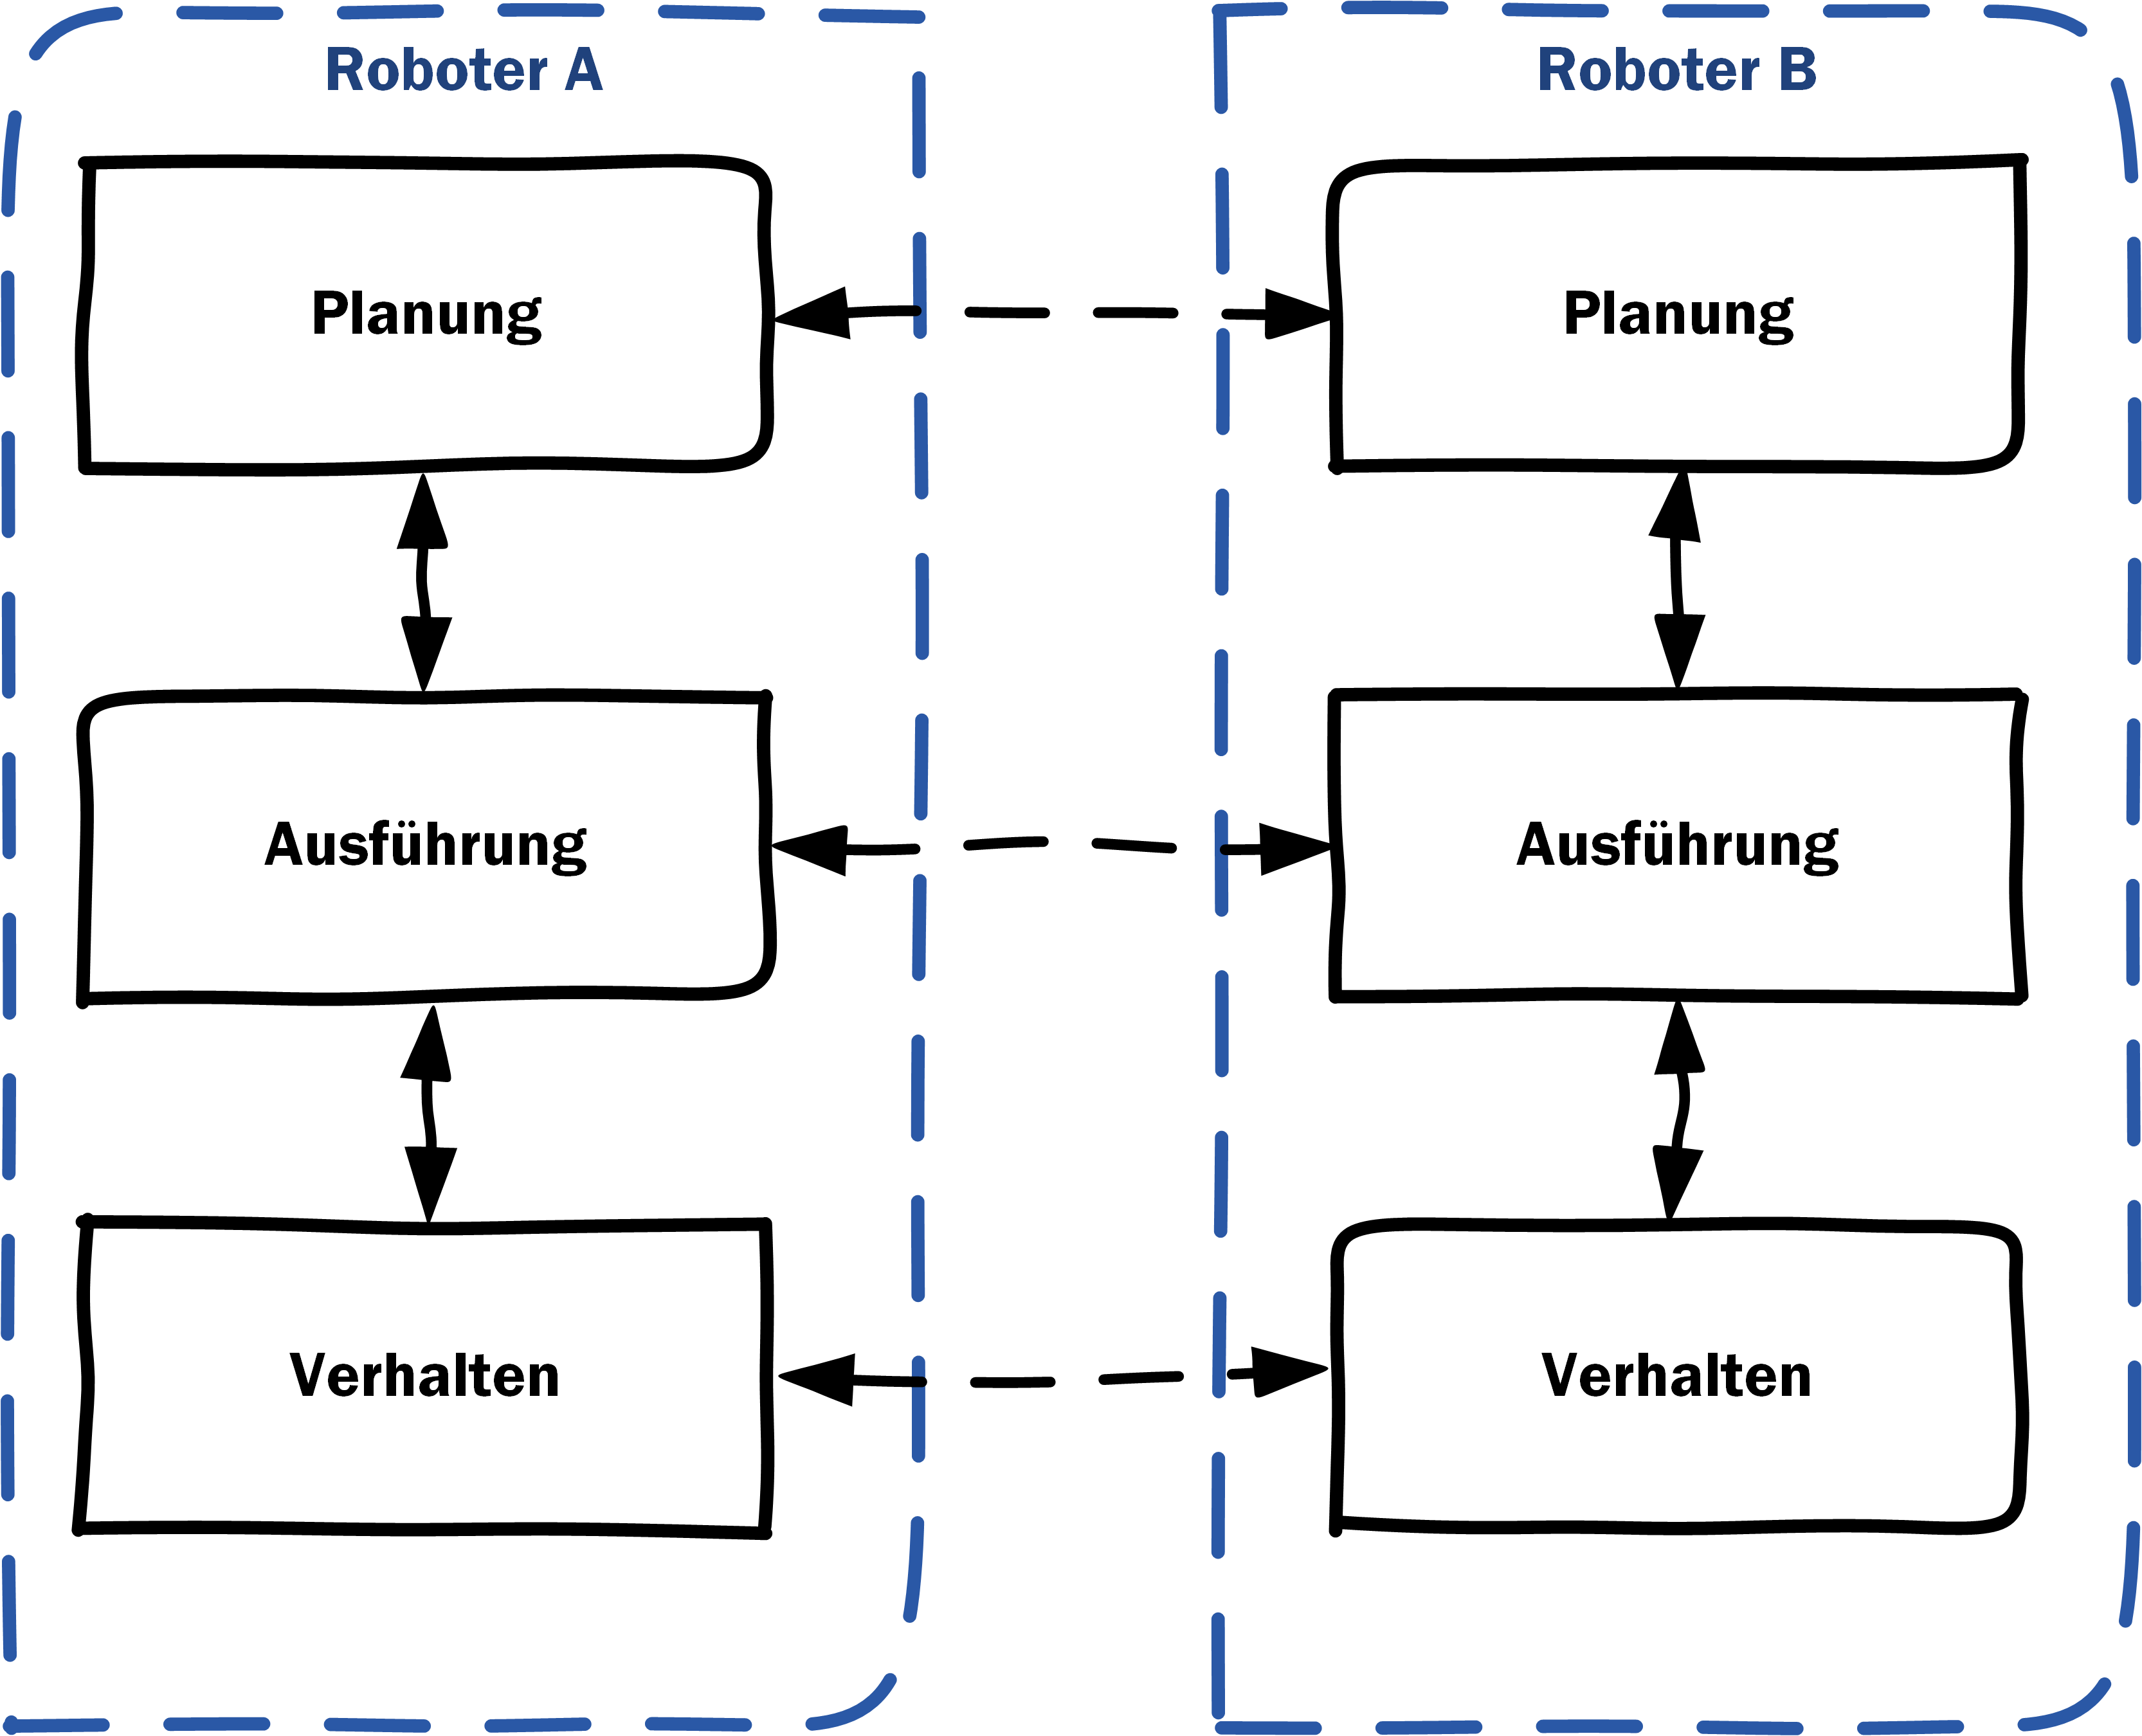
\includegraphics[scale=0.6]{fig/layer}   
%	\caption[Three-Layer Architektur]{Drei Schichten Architektur zur Koordinierung von eng-gekoppelten Systemen. Übernommen aus: \cite{simmons2002layered}}
%	\label{fig:sota-layer}
%\end{figure}

Die schon zitierte Lynne E. Parker leitet die Forschungsgruppe des \textit{Distributed Intelligence Laboratory} an der University of Tennessee. Die zentralen Forschungen der Gruppe befassen sich mit der automatischen Koordination von Roboterteams. 2003 und 2004 präsentierte Parker zwei Arbeiten \cite{parker2003effect} und \cite{parker2004tightly} in denen Netzwerke von über 70 Robotern eng koordiniert wurden. Dabei wurde zwischen sensorarmen und -reichen Robotern unterschieden. Für die enge Kopplung wurde dabei ein Führer-Folger Prinzip gewählt. Als Führer wurden die sensorreichen Roboter ausgewählt. In der Arbeit wurden zwei Tasks bearbeitet. Die erste wurde als Long-Distance-Navigation beschrieben, dabei übernimmt ein Führer die Kontrolle und berechnet einen Weg mit seinen Sensoren. Die sensorarmen Roboter folgen dem Führer. Am Ziel angekommen bauen alle Roboter ein gemeinsames Sensornetzwerk auf und überwachen den Zielraum. Die Roboter innerhalb des Sensornetzwerkes versorgen sich dabei automatisch mit den benötigten Informationen. Die Konfiguration für dieses MRS ist jedoch statisch durch die Entwickler vorgegeben. In der anschließenden Veröffentlichung \cite{parker2005enabling} stellte die Forschungsgruppe \textit{ASyMTRe} (Automated Synthesis of Multi-robot Task solutions through software Reconfiguration) vor. Dieses Konzept, beruhend auf der Schemen Theorie aus \cite{arkin1987motor}, ermöglicht einem MRS eng-gekoppelte Tasks durch Informationsaustausch zu lösen. Dazu werden verschiedene Schemen so miteinander verbunden, dass die Informationen von den Umweltsensoren zu den Motor-Schemen gelangen. ASyMTRe nutzt dazu einen Algorithmus, der alle Informationen für den am wenigsten fähigen Roboter sammelt und diese anschließend an alle verteilt. Anschließend wird der Roboter als Führer ermittelt, der den größten Informationsgehalt bei kleinster Sensorik hat \citep{lundh2006plan} .

\subsubsection{Zusammenfassung}
Dieses Kapitel zeigte Arbeiten und Konzepte rund um das Thema Multi-Robot Systeme auf. In dieser Zusammenfassung sollen die benötigten Informationen für diese Arbeit extrahiert und Entscheidungen für die eigene Entwicklung getroffen werden. In diesem Kapitel wurden zunächst die Begriffe Koordination und Konfiguration durch verschiedene Arbeiten definiert. Außerdem wurden die Begriffe verteilte und zentrale, starke und schwache, sowie enge und lose Koordination erläutert. In den Arbeiten stellte sich heraus, dass zentrale Steuerungen durch einen Single-Point-of-Failure durch Störungen stärker betroffen sind als verteilte Koordination. Diese wiederum benötigt einen größeren Aufwand der Algorithmen und der Konfiguration. Daraus folgt für diese Arbeit, dass ein erster Entwurf eine zentrale Koordinierung haben wird, da der Aufwand beschränkt ist. Jedoch soll eine Schnittstelle für eine verteilte Koordinierung vorgesehen werden. Aus der Literatur ergab sich, dass starke Koordination auf einem Koordinationsprotokoll aufbauen und schwache auf dynamischen Algorithmen, die beteiligte Robotersysteme auswählt. Da in dieser Arbeit nur zwei Roboter verwendet werden und diese zwangsweise miteinander arbeiten müssen ist die Auslegung eines dynamischen Zuweisungsmodell überflüssig, soll aber auch in Form von Schnittstellen für weitere Aufgaben vorgesehen werden. Die Begriffe der eng- und lose-gekoppelten MRS wird durch verschiedene Definitionen unterschiedlich ausgelegt. Für diese Arbeit wird auf die Definition von \cite{kalra2004hoplites} zurückgegriffen. Da in dieser die Begriffe anhand der Zerlegung von Tasks definiert werden, kann die Kategorisierung für dieses System erst nach der Anforderungsanalyse geschehen. Auch die Eingliederung der Tasks in Single-Robot und Multi-Robot Tasks kann erst nach der Anforderungsanalyse erfolgen. Dies betrifft ebenfalls die Entscheidung für Single-Task oder Multi-Task Roboter. Auf ein Rollensystem soll zunächst verzichtet werden, da auch dies für dieses kleine System unnötiger Aufwand ist. Eine Erweiterung die für dieses System vorgesehen ist, beschreibt die Arbeit \cite{davis2003negotiation} mit dem CNP. Die Vergabe der Aufgaben mit Hilfe eines Auktionshauses kann in zukünftigen Entwicklungsschritten auch für komplexere, sogar eng-gekoppelte, MRS genutzt werden. Im folgenden Kapitel wird die Architektur PEIS vorgestellt, die neben Robotersystemen auch weitere Sensoren und Aktoren einschließt. Diese Architektur soll als Ausgangsarchitektur dienen.
%%%%%%%%%%%%%%%%%%%%%%%%%%%%%%%%%%%%%%%%%%%%%%%%%%%%%%%%%%%%%%%%%%%%%%%
%% Related Work
\subsection{Physically Embedded Intelligent Systems - PEIS}
\label{sec:relatedwork-peis}
    
    Andere beschäftigen sich grad mit \ldots



%%%%%%%%%%%%%%%%%%%%%%%%%%%%%%%%%%%%%%%%%%%%%%%%%%%%%%%%%%%%%%%%%%%%%%%
%% Related Work
\subsection{Grasping und Handover - Arbeiten zu Roboterarmen}
\label{sec:relatedwork-handover}
Dieses Kapitel befasst sich mit Arbeiten zu dem Thema Roboterarme. Zunächst wird das Greifen eines Gegenstandes, \textit{Grasping}, aufgezeigt. Dabei werden Arbeiten zum allgemeinen Greifen, zur Erkennung geeigneter Greifpositionen an Gegenständen und Kamera-unterstütztem Grasping aufgeführt. Im Anschluss wird die Thematik der Übergabe, dem zentralen Thema dieser Arbeit, aufgegriffen und Literatur zu Roboter-Mensch Übergaben betrachtet.

\subsubsection{Grasping - Greifen mit einem Roboterarm}
Als Ausgangsarbeit für dieses Thema bietet sich die Arbeit \cite{bicchi2000robotic} an. In dieser werden die Grundlagen des Greifens erläutert. Dabei wird zunächst die menschliche Hand und ihre Verwendungszwecke betrachtet. Der Mensch nutzt seine Hand zur Erkundung, zum Festhalten und zur Manipulation von Objekten. Das Erkunden von Objekten ist der eigene große Forschungsbereich \textit{Haptik} und kann bisher, auf Grund von fehlender Sensorik, in der Robotik nicht vollständig eingesetzt werden. Zwischen dem Festhalten, Fixieren und der Manipulation wird in der Arbeit unterschieden, sowie zwischen dem Manipulieren mit den Fingern und der Manipulation mit dem gesamten Arm. Dies liegt vor allem an den Anwendungs- und Forschungsbereichen. Während das Fixieren eines Objektes, beziehungsweise die Manipulation mit dem gesamten Arm, in der Industrie oft eingesetzt wird, ist die filigrane Arbeit mit den Fingern noch ein Thema der Forschung. Die ersten Arbeiten zu diesem Thema der Robotik gehen auf \cite{asada1979studies}  und \cite{mason1985robot} zurück. Neben dem Greifen mit den Fingern der Hand gibt es auch Griffe mit dem kompletten Arm, bezeichnet mit \textit{whole arm graps} \citep{townsend1988effect}, \citep{bicchi1994problem} und \textit{power grasps} (\citep{mirza1990force}) \citep{bicchi2000robotic}. 

Das Greifen unterliegt physischen Grenzen. Dabei wird der Griff, beziehungsweise das Halten, unter anderem durch den Kraftvektor und dem Haftkoeffizienten beeinflusst. Ein Griff wird durch $N$ Kontakte beschrieben. Dabei wird angenommen, dass alle Kontakte punktuell sind. Auch ein Kontakt auf einer Linie oder Oberfläche wird durch zwei oder mehr Punktkontakte abgebildet. Die Literatur unterscheidet diese Kontakte in reibungslose, reibungsbedingte oder weiche Punktkontakte \citep{salisbury1983kinematic}. Ein reibungsloser Kontakt kann nur eine Kraft entlang der gemeinsamen Normalen erzeugen. Ein reibungsbedingter kann neben der normalen auch eine tangentiale Kraft und ein weicher Kontakt zusätzlich ein Drehmoment erzeugen. Die Kontaktart ist abhängig von den Oberflächeneigenschaften des Greifers und des Objektes. Bei einer gummiähnlichen Oberfläche des Greifers wird der Kontakt als weich modelliert. Haben Greifer und Objekt beide harte und raue Oberflächen wird ein reibungsbedingter Kontakt angenommen. Sind die Kontaktstellen auf Greifer und Objekt glatt und ist ein kleiner Reibungskoeffizient gegeben, gilt der Kontakt als reibungslos \citep{bicchi2000robotic}.


Neben dem Greifen selbst existiert auch die Problematik des Greifpunktes. Also der Stelle am Objekt, an welcher der Greifer ansetzt. Dazu existieren verschiedene Arbeiten. Die ersten zu diesem Thema waren die Arbeiten \cite{kamon1996learning}, \cite{coelho2001developing} und \cite{bowers2003manipulation}. In diesen werden mit Hilfe von Sensoren planare 2D-Objekte gegriffen. Ergebnisse mit 3D-Objekten erreichte die Arbeit \cite{saxena2008robotic}. Dabei werden zunächst mit maschinellem Lernen und gelabelten Testdatensätzen gute Griffpunkte für 3D-Objekte angelernt. Anschließend kann der Algorithmus unbekannte 3D-Objekte bewerten und die besten Griffpunkte finden. Diese Grundlagenforschung wird in der Arbeit \cite{maitin2010cloth} genutzt um an unbekannten 3D-Objekten aus Stoff Ecken zum Greifen und Zusammenlegen zu finden. In dieser werden vor allem Ansätze nach dem RANSAC-Verfahren gewählt, um bestimmte Strukturen gezielt zu finden. Für weitere Informationen lassen sich in der Literatur noch viele verschiedene Anwendungsfälle und Ansätze zum Greifen finden.

\subsubsection{Handover - Übergabe zwischen zwei Systemen}
Die Übergabe zwischen zwei Systemen ist eine häufige Interaktion im Alltag. Dieses betrifft oft die Manipulation eines Objektes. Die Arbeit \cite{huber2008human} beschäftigt sich mit der Übergabe zwischen Mensch und Roboter und beinhaltet zunächst eine Analyse einer Übergabe zwischen zwei Menschen. Dabei stellt sich folgende Aktionsreihenfolge für eine Übergabe heraus \citep{huber2008human}:

\begin{enumerate}
	\item Der Geber nimmt das Zielobjekt
	\item Der Geber bewegt die Hand Richtung Übergabeposition
	\item Der Nehmer bewegt die Hand Richtung Übergabeposition
	\item Transaktion
	\item Beide nehmen ihre Hände zurück
\end{enumerate}

Eigene Beobachtungen vom Mensch-Mensch Übergaben ergaben, dass diese Form der Übergabe nur eine Interaktionsart ist und als \textit{Geben} bezeichnet werden kann, da die Interaktion vom Geber ausgeht. Eine Alternative dazu stellt das \textit{Nehmen} dar, bei dem die Interaktion vom Nehmer ausgeht. Eine optimierte dritte Interaktionsart wäre eine synchrone Bewegung beider Akteure, bei der eine Verzögerung durch die Reaktionszeit des Interaktionspartners entfällt.

In der Robotik existieren mehrere Arten der Übergabe. Diese unterscheiden sich anhand des Interaktionspartners und des Anwendungsfeldes. 
In der Industrie, zum Beispiel dem Automobilbau, werden die Werkstücke nicht direkt zwischen den einzelnen Robotern übergeben, sondern befinden sich auf einem Förderband. Dieses fährt das Werksstuck auf eine definierte Position und die einzelnen Roboter führen ihren Arbeitsschritt aus. Anschließend wird das Werksstück zur nächsten Station gebracht. Eine weitere Art der Übergabe ist die Mensch-Roboter-Interaktion. Dieses Thema ist ein weitverbreitetes Thema mit vielen Aspekten. So beschäftigen sich die Arbeiten \cite{huber2008human} und \cite{shibata1995experimental} mit dem Timing-Verhalten, \cite{mainprice2010planning} und \cite{kulic2005safe} befassen sich mit der sicheren Planung von Übergabe-Interaktionen. Weitere Arbeiten (unter anderem \cite{prada2014implementation} und \cite{basiliapproach}) beschäftigen sich mit den Reaktionen auf menschliche Aktionen, wie Gesten (zum Beispiel: Handfläche nach oben geöffnet als Geste fürs Nehmen) und Veränderungen während der Übergabe.

In dieser Arbeit steht jedoch die Roboter-Roboter-Übergabe im Fokus. Dieses Thema ist in der Literatur nicht vorhanden oder wird nur als Randaspekt erwähnt.
\clearpage

%%%%%%%%%%%%%%%%%%%%%%%%%%%%%%%%%%%%%%%%%%%%%%%%%%%%%%%%%%%%%%%%%%%%%%%
%% Aufbau
%%%%%%%%%%%%%%%%%%%%%%%%%%%%%%%%%%%%%%%%%%%%%%%%%%%%%%%%%%%%%%%%%%%%%%%
%% Related Work
\section{Laboraufbau}
\label{sec:basic-aufbau}
    
Dieses Kapitel befasst sich mit dem Aufbau der Versuchsanlage und der verwendeten Hardware. Dabei werden die Aspekte des räumlichen Aufbau genauso betrachtet wie die Netzwerkinfrastruktur und die genutzten Roboter und Sensoren.



\subsection{Aufbau Teststand}
Der Aufbau vom Teststand ist in den beiden Abbildungen \ref{fig:basic-aufbau-teststand} in der Draufsicht und \ref{fig:basic-aufbau-teststandh} in der Seitenansicht dargestellt. Rote Flächen stellen die Wände dar. Tische sind in blau gezeichnet. Die grüne Fläche ist die Arbeitsplatte auf welcher der Roboter \textit{Dummy} (orange) fixiert ist. Türkise Objekte stellen Geräte wie Kameras und Monitore dar.

 \begin{figure}[H]
 	\centering
 	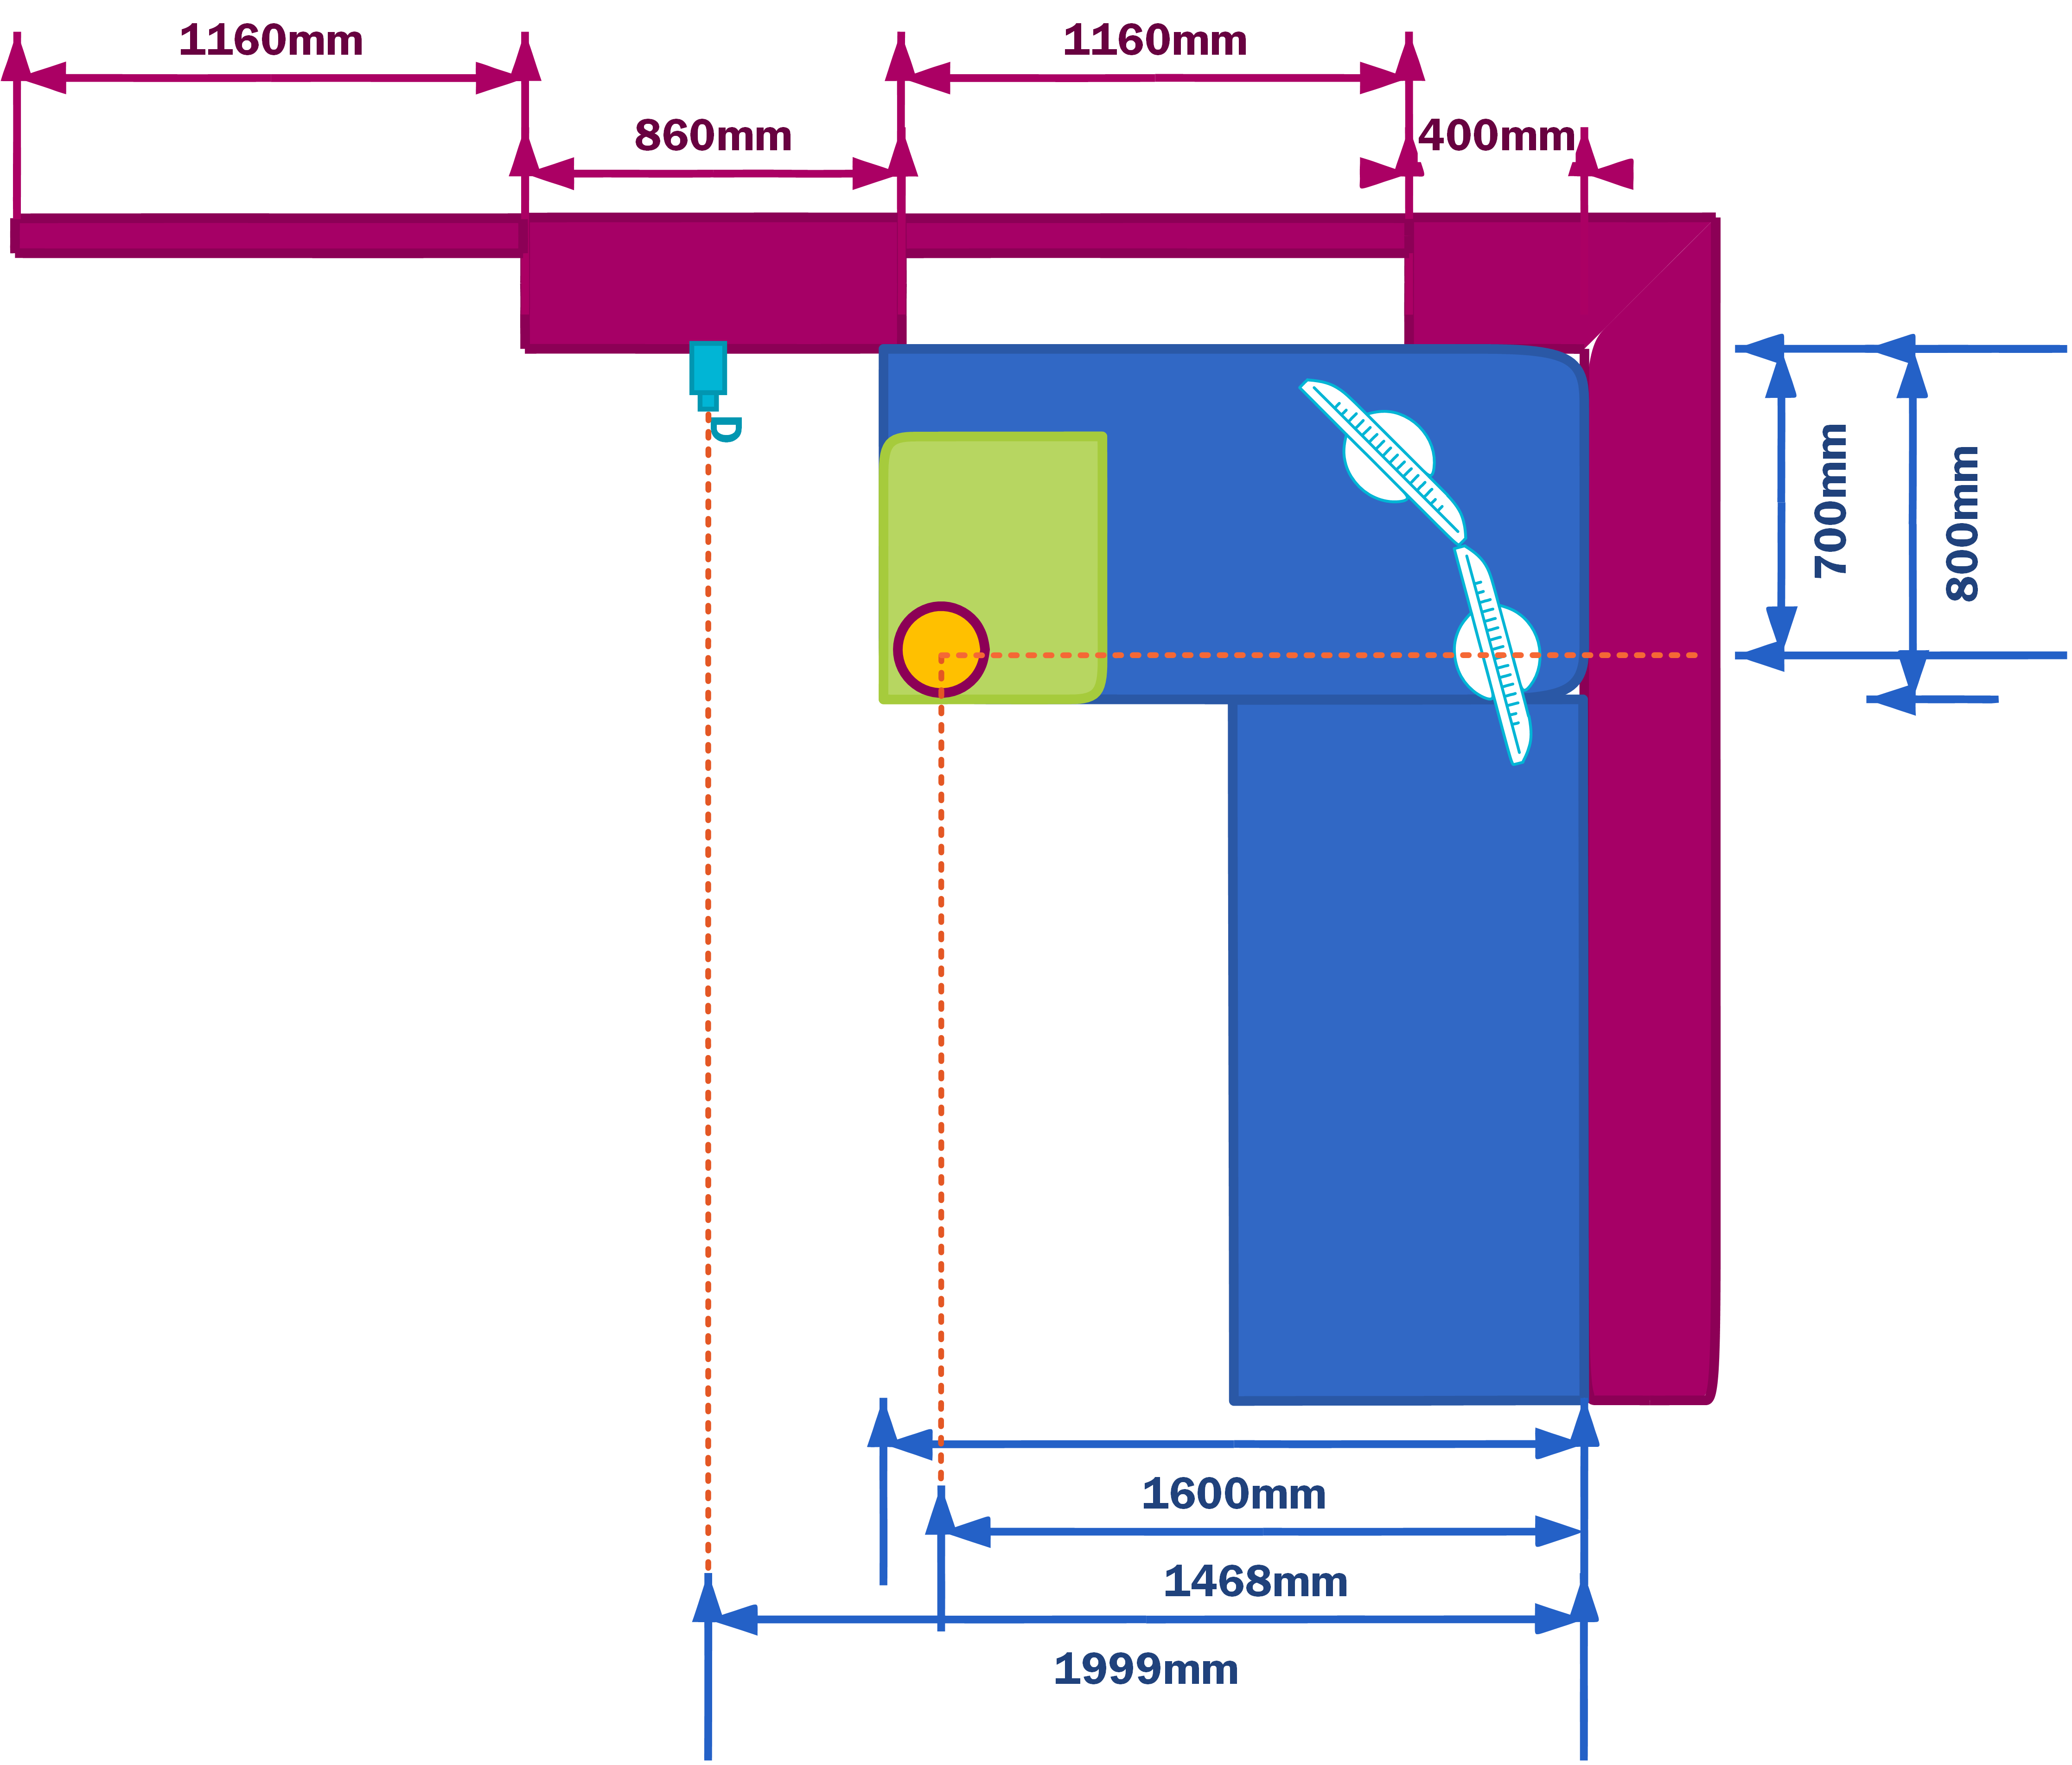
\includegraphics[scale=0.8]{fig/ZeichnungRaum}   
 	\caption[Aufbau Teststand: Draufsicht]{Der Aufbau aus der Draufsicht vom Teststand. Rot: Wände, Blau: Tische, Grün: Arbeitsplatte Roboter, Orange: Roboter, Türkis: Geräte}
 	\label{fig:basic-aufbau-teststand}
 \end{figure}
 
 
 
  \begin{figure}[h]
  	\centering
  	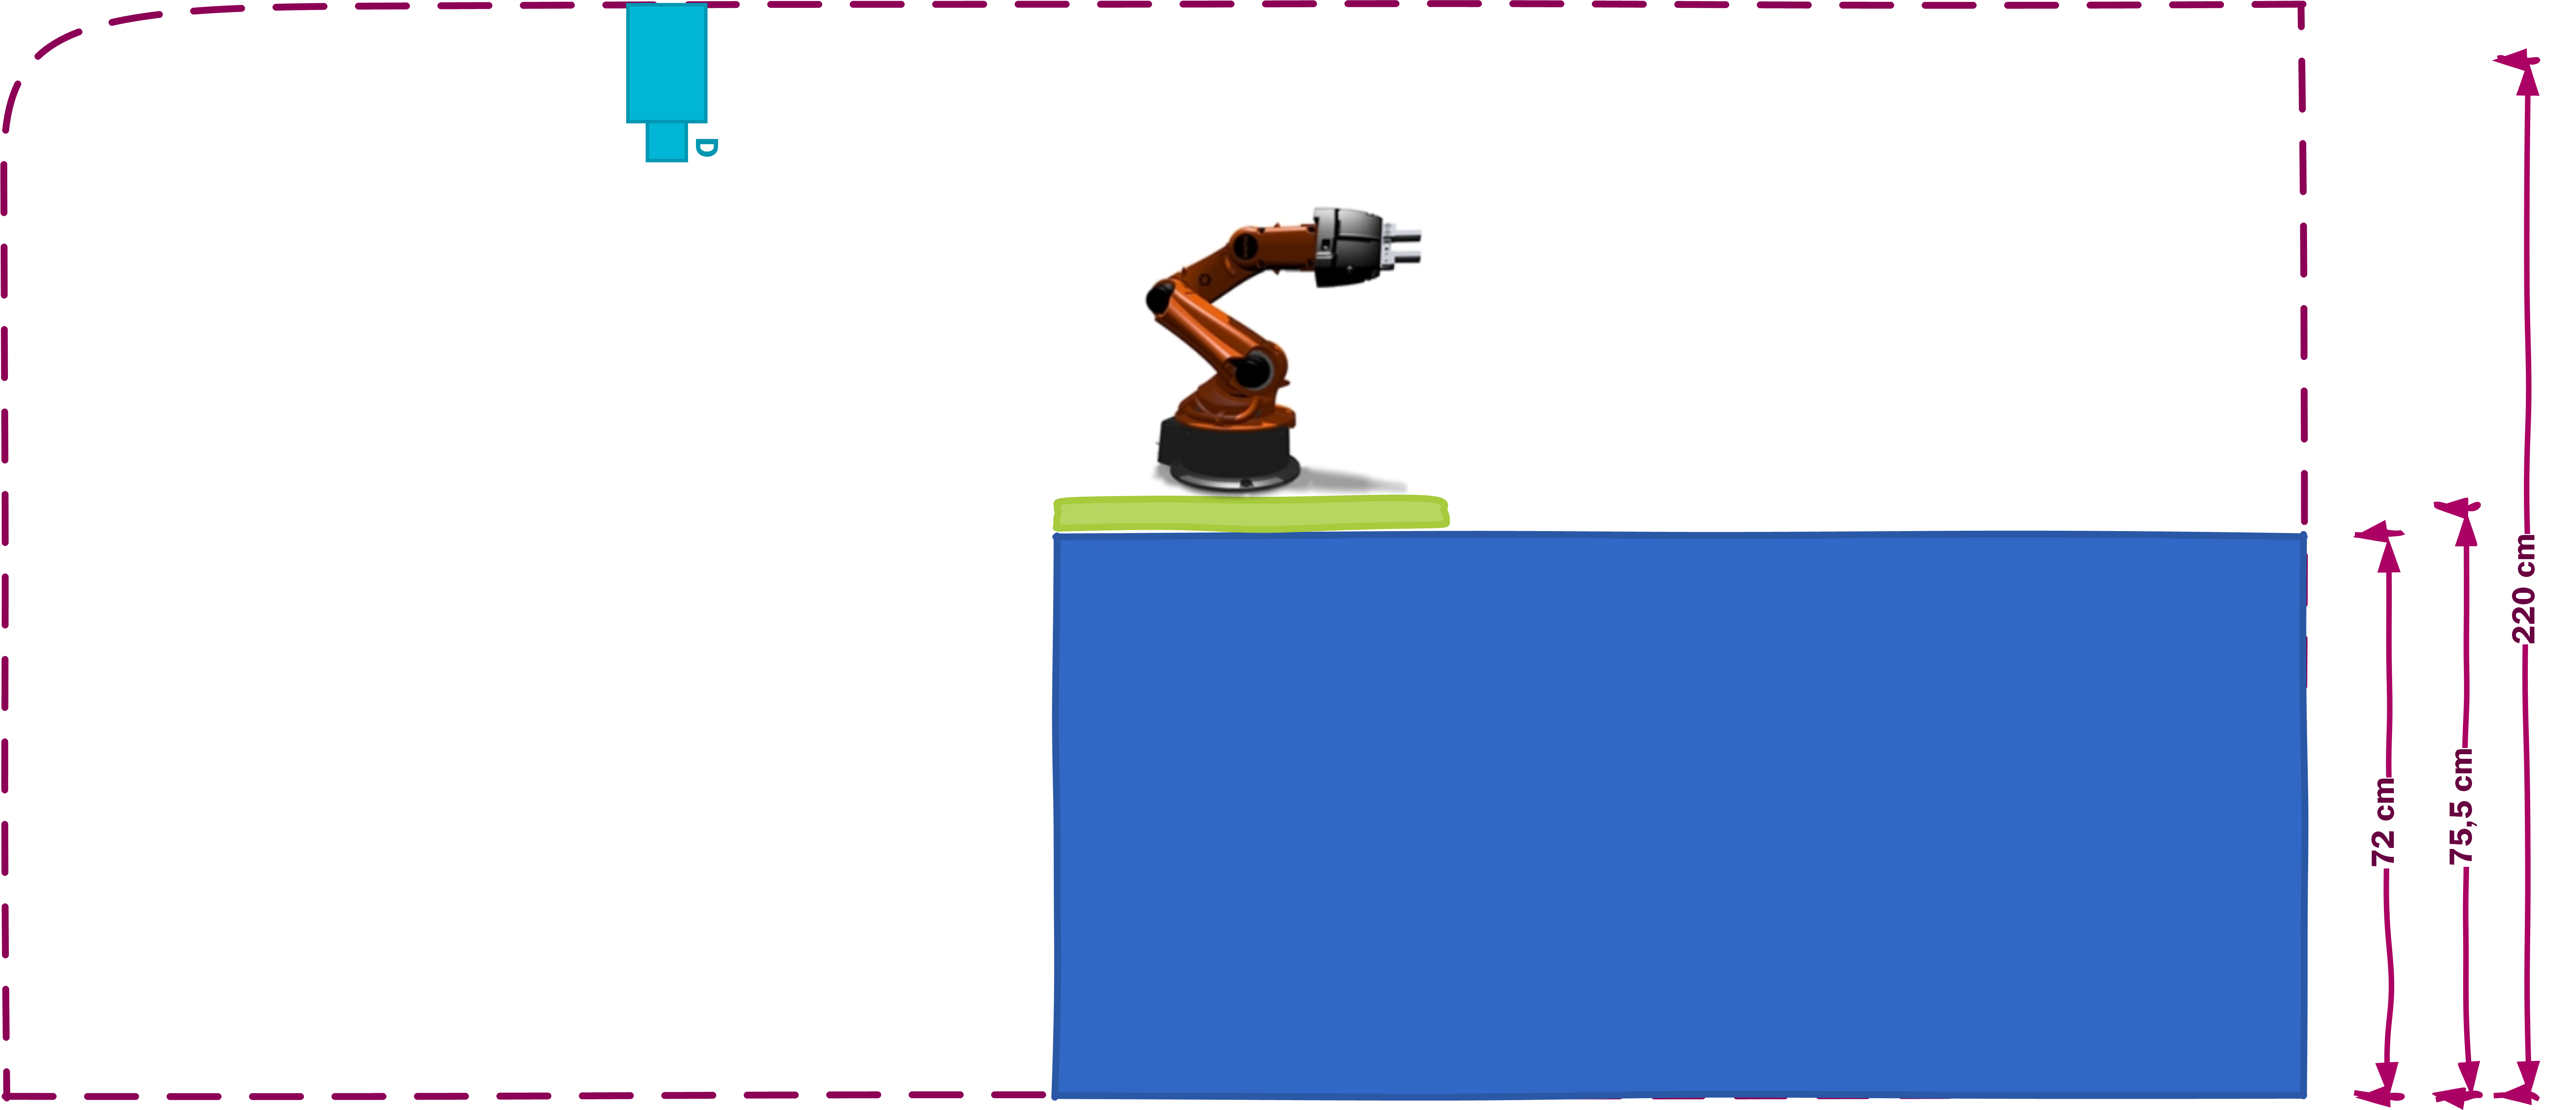
\includegraphics[scale=0.5]{fig/ZeichnungRaumH}   
  	\caption[Aufbau Teststand: Seitenansicht]{Der Aufbau aus der Draufsicht vom Teststand. Rot gestrichelt: Wände, Blau: Tische, Grün: Arbeitsplatte Roboter, Orange: Roboter, Türkis: Kamera}
  	\label{fig:basic-aufbau-teststandh}
  \end{figure}

\subsection{YouBot}
In dieser Arbeit werden zwei Roboter genutzt. Bei beiden handelt es sich um YouBots der Firma Kuka. Diese wurden 2010 erstmals auf der Automatica in München vorgestellt. Kuka ist ein deutscher Hersteller von Industrierobotern mit Sitz in Augsburg.Kuka hat aber auch Erfahrung im Bau von experimentellen Robotern wie etwas die Arme für Justin, einem Service-Roboter.

Die beiden YouBots unterscheiden sich beim Aufbau. YouBot 1 besteht aus einem Manipulator mit Gripper, YouBot 2 besteht aus Manipulator mit Gripper und mobiler Plattform mit omnidirektionalen Rollen. Zur besseren Unterscheidung und zur Lesbarkeit dieser Arbeit haben beide Roboter einen Namen bekommen. YouBot 1 entspricht dabei \textbf{Dummy}, YouBot 2 ist \textbf{Rose}. Im Weiteren Verlauf der Arbeit werden nur noch diese Namen genutzt um eine Verwechslung zu vermeiden.


\subsubsection{Manipulator}
 Die Roboterarme von Dummy und Rose sind eine offene kinematische Kette mit fünf Joints, die von der Basis aufsteigend numeriert sind. An Joint 5 sind die Gripper montiert, diese bestehen aus zwei individuellen Fingern, die linear auf einer Achse bewegt werden können.

Joint 1 und Joint 5 sind zwei Drehgelenke um die Z-Achse, die bei ausgestreckter Haltung (Candle-Pose) parallel liegen. Joint 2, 3 und 4 sind Kippgelenke um die X-Achse, die immer parallel liegen. Durch diese Konstellation ergeben sich für den kompletten Arm fünf Freiheitsgrade (5-DOF). Durch die Einschränkung der Achsen auf die X- und Z-Achsen der einzelnen Joints ist ein seitlicher Griff bei $x_{base} = 0$ oder $y_{base} = 0$ nicht möglich. Die Höhe in Candle-Pose beträgt inklusiv Gripper 655mm. Die einzelnen Abstände lassen sich der Grafik \ref{fig:basic-aufbau-youbot-kinematik} entnehmen.

\begin{figure}[H]
	\centering
	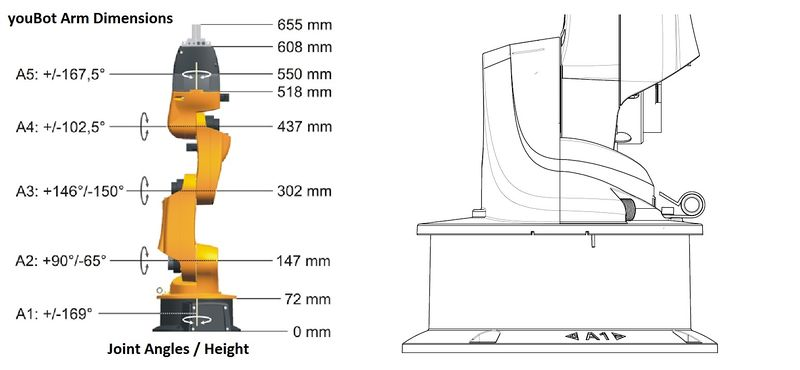
\includegraphics[scale=0.8]{fig/kukaarm_1}   
	\caption[YouBot Arm Kinematik]{YouBot Arm Kinematik. Links: Detailierter Mechanismus mit Joint und Link Angaben. Rechts: Vergrößerte Darstellung der Basis. Bildquelle: \cite{monikaflorekjasinska2015}}
	\label{fig:basic-aufbau-youbot-kinematik}
\end{figure}



 
 Tabelle \ref{tab:basic-aufbau-youbot-joints} stellt noch einmal den Drehbereich aller Joints dar. Dabei sind neben Bezeichner auch die minimalen und maximalen Winkel, sowie die Winkelgeschwindigkeiten. Eine Besonderheit stellt Joint 3 dar, durch den Aufbau bedingt wurde die Achse innerhalb der Treiber gespiegelt, sodass die Winkel um den 0° Punkt gespiegelt wurden. In der Tabelle und den folgenden Zeichnungen ist diese Spiegelung nicht beachtet.
 
   \begin{table}[H]
   	\begin{tabular}{|c|c|c|}
   		\hline Bezeichnung & Max./Min. Winkel & Winkelgeschwindigkeit (rad / s) \\ 
   		\hline Joint 1 & $\pm$ 2.94 & $\frac{\pi}{2}$  \\ 
   		\hline Joint 2 & + $\frac{\pi}{2}$ / -1.13  & $\frac{\pi}{2}$ \\ 
   		\hline Joint 3 & +2.54 /-2.63 & $\frac{\pi}{2}$ \\ 
   		\hline Joint 4 & $\pm$1.78 & $\frac{\pi}{2}$ \\ 
   		\hline Joint 5 & $\pm$2.91 & $\frac{\pi}{2}$ \\ 
   		\hline 
   	\end{tabular}
   	\caption[YouBot Arm Joints]{YouBot Arm Joints. Quelle: \cite{monikaflorekjasinska2015}}
   	\label{tab:basic-aufbau-youbot-joints}
   \end{table}
   
   Der Arbeitsraum des YouBot Arms beschränkt sich durch die Joints. Die Grafiken \ref{fig:basic-aufbau-youbot-workspace} und \ref{fig:basic-aufbau-youbot-workspace-top} stellen den Arbeitsbereich eingeschränkt dar. Die Darstellung \ref{fig:basic-aufbau-youbot-workspace} zeigt mit Hilfe von Konturen die einzelnen Bahnen unter Beschränkung der Joints, sowie der End-Effektor Ausrichtung.  Die äußerste Kontur gibt die maximale Reichweite für den End-Effektor an. Die Z-Achse steht dabei orthogonal zur Tangente an der Konturposition. Abbildung \ref{fig:basic-aufbau-youbot-workspace-top} gibt eine Draufsicht auf den Arbeitsraum. Durch die Beschränkung von Joint 1 befindet sich ein toter Winkel im "Rücken" der Arms. Dieser kann durch einen Überschlag des ganzen Arm, insbesondere Joint 2 und 3, und einer 180 \textdegree Drehung von Joint 1 dennoch erreicht werden. Dies wird durch den linken Bereich in Abbildung \ref{fig:basic-aufbau-youbot-workspace} klar.
   
   \begin{figure}
   	\centering
   	\subfigure[YouBot Arm Arbeitsraum. Reichweite der einzelnen Gelenk und einzelne Abmessung der Links und Link-Offsets. Einheitslose Angaben sind in mm.]{%
   		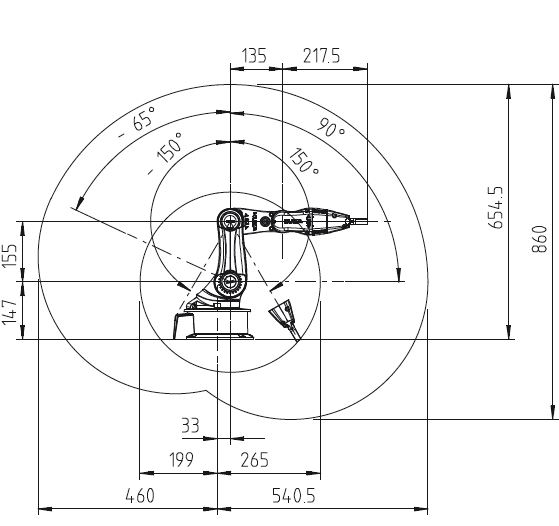
\includegraphics[scale=0.55]{fig/kukaarm_2}
   		\label{fig:basic-aufbau-youbot-workspace}}
   	\hfill
   	\subfigure[Draufsicht YouBot Arm Arbeitsraum.]{%
   		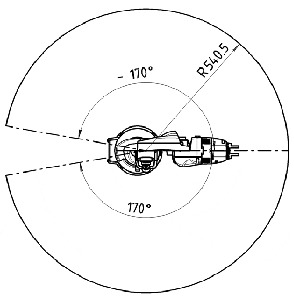
\includegraphics[scale=0.55]{fig/kukaarm_3}
   		\label{fig:basic-aufbau-youbot-workspace-top}}
   	\caption{Arbeitsraum YouBot. Bilderquelle:\cite{monikaflorekjasinska2015}}
   	\label{fig:basic-aufbau-youbot-workspace-full}
   \end{figure}

\subsubsection{Mobile Plattform}
Rose besitzt neben dem Arm noch eine mobile Plattform. Diese ist 590 mm lang, 380 mm breit und 140 mm hoch. Die Plattform hat vier Räder mit einem Durchmesser von 47.5 mm. Jedes Rad lässt sich getrennt ansteuern. Bei den Rädern handelt es sich um Mecanum-Räder, die eine Steuerung in alle Richtungen ermöglicht. Dazu sitzen auf jeder Felge sechs drehbare tonnenförmige Rollen die im Winkel von 45° zur Achse des Rades angebracht sind. Damit Omni-Direktionale Bewegungen möglich sind werden die Räder abwechselnd zum Nachbar auf +45° oder -45° angeordnet. Die minimale Geschwindigkeit der Plattform beträgt $0.01\frac{m}{s}$, die maximale  $0.8\frac{m}{s}$. Abbildung \ref{fig:basic-aufbau-youbot-base} zeigt den Aufbau und Abmessungen der Plattform. 

\begin{figure}[H]
	\centering
	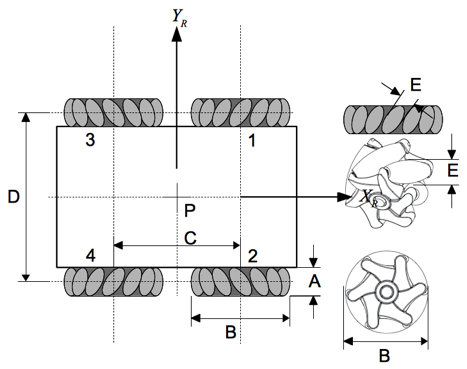
\includegraphics[scale=0.8]{fig/kukabase}   
	\caption[YouBot Base]{YouBot Base. A = 74.87 mm, B = 100 mm, C = 471 mm, D = 300.46 mm E = 28 mm. Die Bodenfreiheit der Plattform beträgt 20 mm. Bildquelle: \cite{monikaflorekjasinska2015}}
	\label{fig:basic-aufbau-youbot-base}
\end{figure}

Die Plattform von Rose ist modifiziert und besitzt eine Aufsatzplatte. Diese dient zur Montage zusätzlicher Sensoren und zur Schutz der Räder bei Kollisionen. Diese ist 600 mm lang und 396 mm breit. Durch die Abstandsbolzen und die Dicke der Platte (5 mm) erhöht sich die Plattform auf 150 mm (siehe Abbildung \ref{fig:basic-aufbau-youbot-base_side}).  

 \begin{figure}[H]
 	\centering
 	\subfigure[Seitenansicht mobile Plattform mit Sensorplatte]{%
 		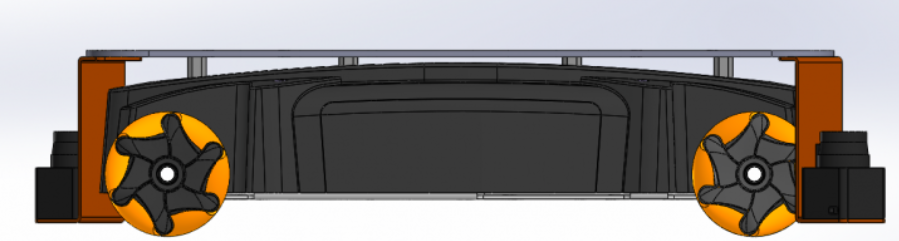
\includegraphics[scale=0.55]{fig/base2}
 		\label{fig:basic-aufbau-youbot-base_side}}
 	\subfigure[Draufsicht mobile Plattform mit Sensorplatte]{%
 		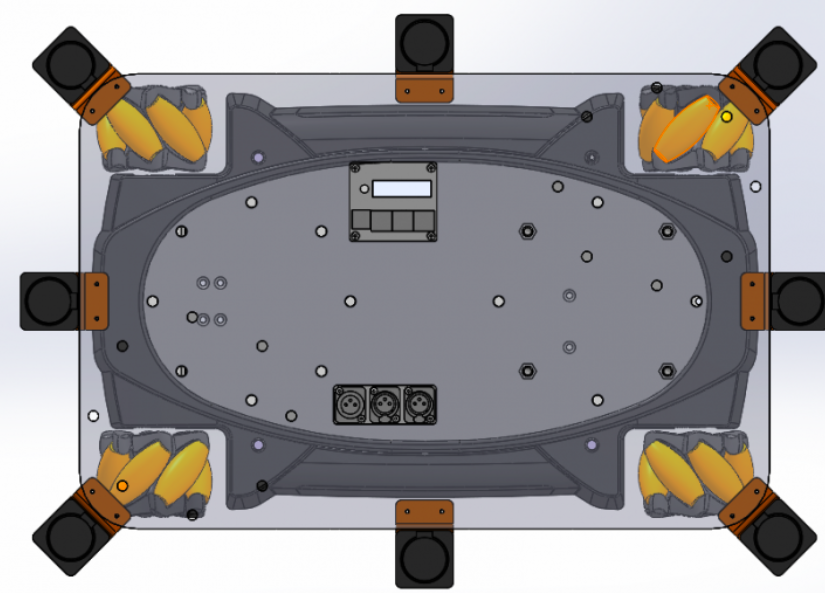
\includegraphics[scale=0.55]{fig/base3}
 		\label{fig:basic-aufbau-youbot-base-top}}
 	\caption{Mobile YouBot Plattform mit Sensorplatte. Bilderquelle:\cite{kuka2015}}
 	\label{fig:basic-aufbau-youbot-base-full}
 \end{figure}

\subsubsection{Rechner}
Für die Rechenleistung der beiden Roboter sorgen neben den verbauten, eingebetteten Boards zwei Computer mit Linux Betriebssystemen.
Der für Rose zuständige PC ist ein Mini-ITX und in der mobilen Plattform eingebaut. Dieser läuft mit einem Intel Atom D510 Dual Core mit 1.66 GHz als CPU und 2 GB DDR2 RAM. Als Festplattensystem ist eine 32 GB SSD verbaut. Der Rechner stellt einige IO-Schnittstellen zur Verfügung: sechs USB 2.0, ein VGA und zwei LAN Anschlüsse sind nutzbar. Dabei ist ein LAN Anschluss für den Ethercat-Anschluss der Plattform belegt. Diese wiederum bringt nochmal zwei LAN Anschlüsse mit. Der Rechner für Dummy ist ein TODO %TODO Dummy PC

Weitere Details zu den Armen, der Plattform oder den Rechnern befindet sich im Anhang \ref{app:daten}.

\subsection{Sensoren}
\label{sec:aufbau-sensoren}
Für die Erkennung von Objekten und der Positionierung im Raum sind mehrere Sensoren nötig. In dieser Arbeit wird dabei auf das Kamerasystem Asus XTion Pro Live und auf einen Laserscanner Hokuyo URG-04LX-UG01 zurückgegriffen.

\subsubsection{Asus XTion Pro}
Die XTion Pro ist ein Tiefenkamerasystem von Asus. Es besteht aus einer RGB-Kamera, einer Tiefen-Kamera und zwei Mikrophonen. Die Kamera wurde von Prime Sense entwickelt und ist eine um gelabelte Microsoft Kinect. Die XTion ist kleiner und leichter als die Kinect und damit besser für die Robotik geeignet. Angeschlossen wird die XTion mit einem USB Kabel und betrieben mit dem ROS Paket OpenNI2. Der Node published eine PointCloud mit RGB Daten, sowie eine PointCloud für die Tiefenkamera, als auch Bilder der RGB Kamera.

Das Sichtfeld der Kamera beträgt Horizontal 58\textdegree, 45\textdegree Vertikal und 70\textdegree Diagonal. Die Auflösung der Tiefenkamera beträgt bei 30 Frames pro Sekunde 640x480 und bei 60 FPS 320x240. Die Auflösung des RGB-Bildes 1280x1024. Die nutzbare Distanz der Tiefenkamera beträgt zwischen 800 mm und 3500 mm.\cite{asus2015} Diese Distanz schränkt die Nutzbarkeit der Kamera ein, so ist sie nicht für eine visuelle Unterstützung der Gripper geeignet, wenn sie an diesen montiert ist, da die Distanz zwischen Kamera und Gripper kleiner 800 mm ist.

\begin{figure}[H]
	\centering
	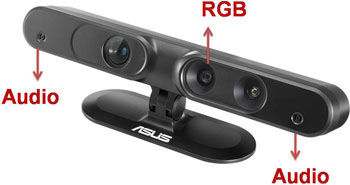
\includegraphics[scale=0.8]{fig/xtion1}   
	\caption[Asus Xtion Pro Live]{Asus XTion Pro Live. Bildquelle: \cite{asus2015}}
	\label{fig:aufbau-xtion}
\end{figure}

\subsubsection{Hokuyo URG-04LX-UG01}
Der URG-04LX-UG01 ist ein optischer Abstandsmesser. Dieser kann Entfernungen in einer zirkulären Ebene messen. Entwickelt wurde er von der Firma Hokuyo, welche neben dem URG noch weitere, ähnliche Sensoren anbietet, die andere Reichweiten und Sichtfelder abdecken. Die Sensoren nutzen zur Messung der Entfernung eine Infrarot-Diode mit einer Wellenlänge von 785 nm. Die Distanz wird mit Hilfe der Phasenverschiebung berechnet. Diese Technik reduziert den Einfluss durch das Oberflächenmaterial des gemessenen Objektes. Versorgt wird der Sensor mit 5V DC, welche über den USB-Anschluss angelegt werden. Da die Startleistung des Sensors die maximale Abgabeleistung eines einzigen USB-Anschluss überschreitet, müssen ein Y-USB-Kabel und zwei USB-Anschlüsse genutzt werden. Angesteuert wird der Sensor mit dem ROS-Paket Hokuyo-Node, welche eine PointCloud published.

Der URG-Sensor hat eine Reichweite von maximal 4000 mm und benötigt für eine Messung 100 ms, was einer Messrate von 10 FPS entspricht. Das Sichtfeld beträgt 240\textdegree. Die minimale Graduelle Auflösung beträgt 0.36\textdegree. Dadurch ergeben sich die ungefähren Disparitäten von 20 mm bei 2000 mm und maximal 40 mm bei 4000 mm Radius. Die Ungenauigkeit beträgt maximal 3 Prozent des gemessenen Wertes, was bei der maximalen Reichweite von 4000 mm einer Abweichung von 120 mm entspricht.\cite{maeda2009}

 \begin{figure}[H]
 	\centering
 	\subfigure[Produktbild. Bildquelle: \cite{nowak2015}]{%
 		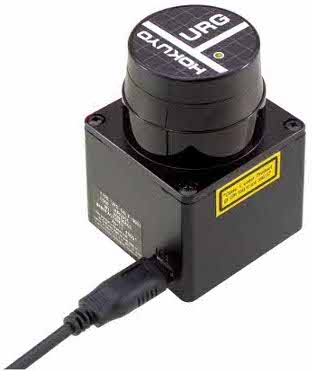
\includegraphics[scale=2.5]{fig/hok2}
 		\label{fig:aufbau-hok2}}
 	\subfigure[Schema: Reichweite und Sichtfeld. Sichtfeld in Messpunktsektoren (MP) unterteilt. Verändert nach: \cite{maeda2009}]{%
 		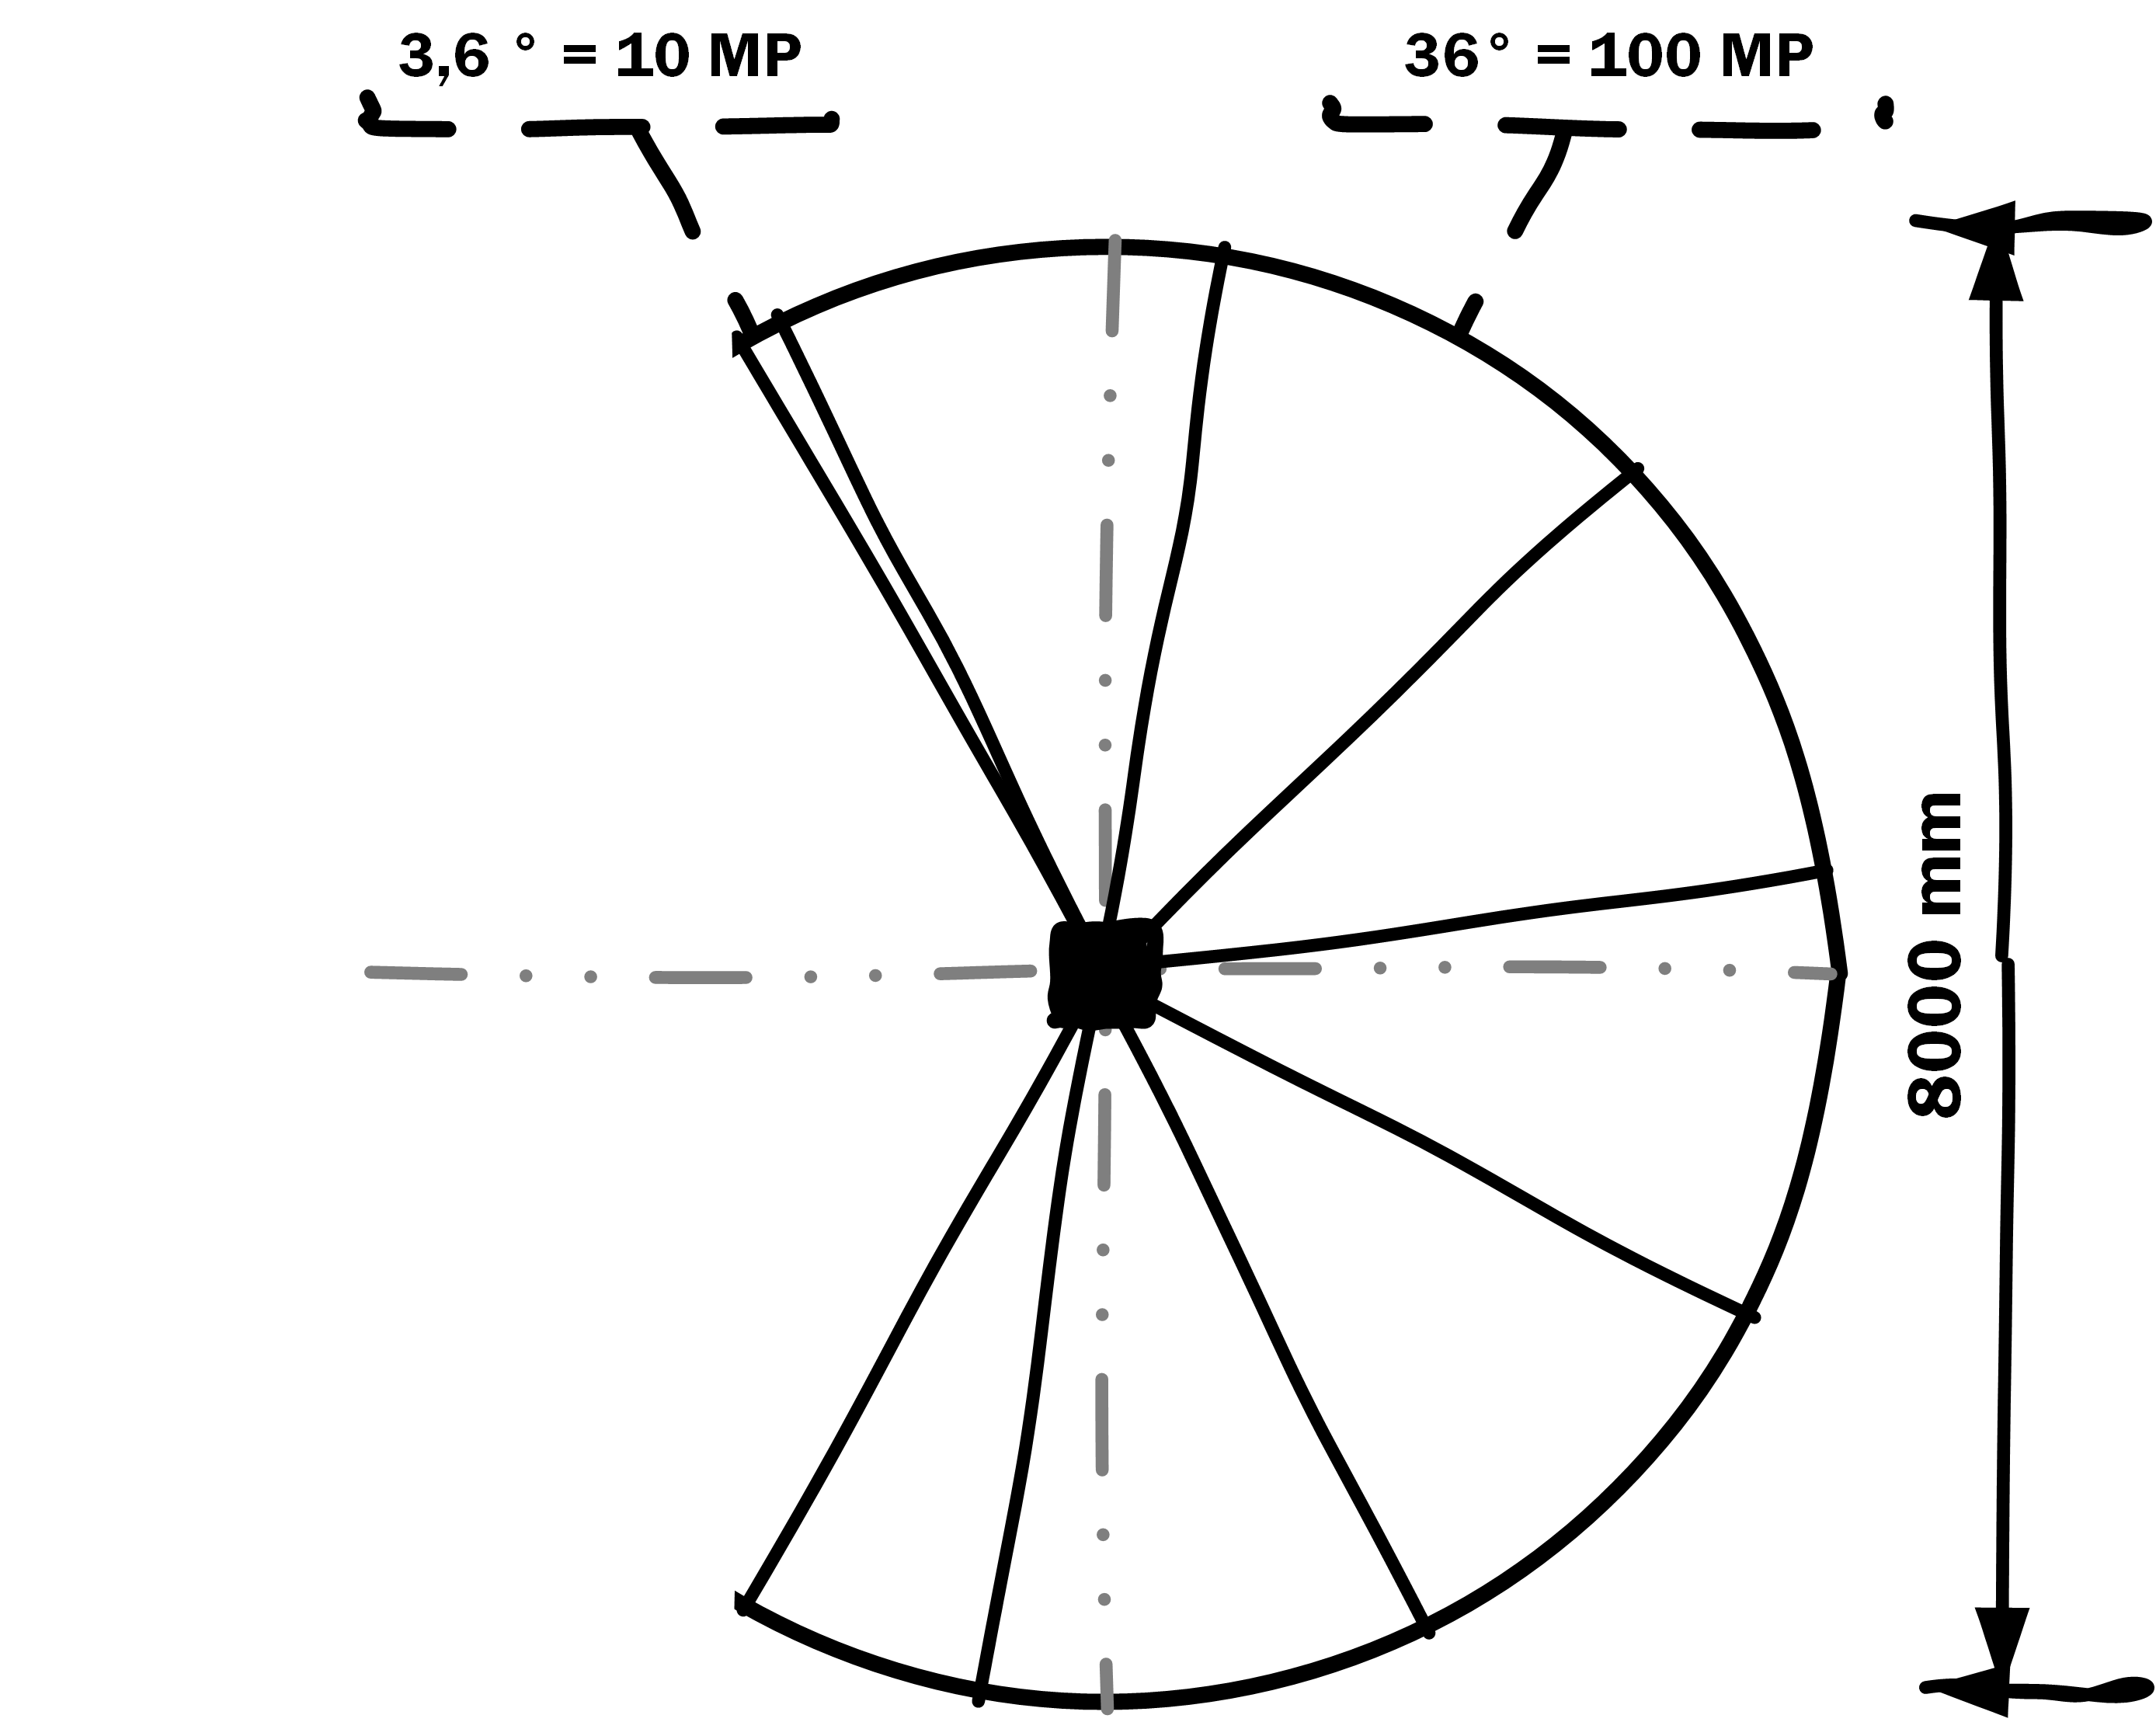
\includegraphics[scale=0.7]{fig/hok1}
 		\label{fig:aufbau-hok1}}
 	\caption{Hokuyo URG-04LX-UG01}
 	\label{fig:aufbau-hok}
 \end{figure}

\subsubsection{Argos 3D - P100}
Ein weiterer Tiefensensor ist die Argos 3D – P100 von Bluetechnix. Diese arbeitet mit dem Time of Flight (ToF) Prinzip. Der Sensor wird mit einem USB-Kabel angesteuert, benötigt aber noch eine weitere Stromzufuhr. Der Sensor kann aus ROS mit einem eigenen Node angesprochen werden. Der Sensor hat eine Reichweite zwischen 100 mm und 3000mm. Die Framerate beträgt bis zu 160 FPS bei ein Auflösung von 160 x120. Das Sichtfeld beträgt 90 \textdegree.\citep{bluetechnix2015}

\begin{figure}[H]
	\centering
	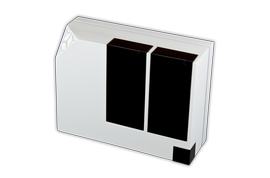
\includegraphics[scale=0.8]{fig/argos3d}   
	\caption[Argos 3D - P100]{Argos 3D - P100. Bildquelle: \cite{bluetechnix2015}}
	\label{fig:aufbau-argos3d}
\end{figure}

\subsubsection{Netzwerk- und Sensoranbindung}

\begin{figure}[H]
	\centering
	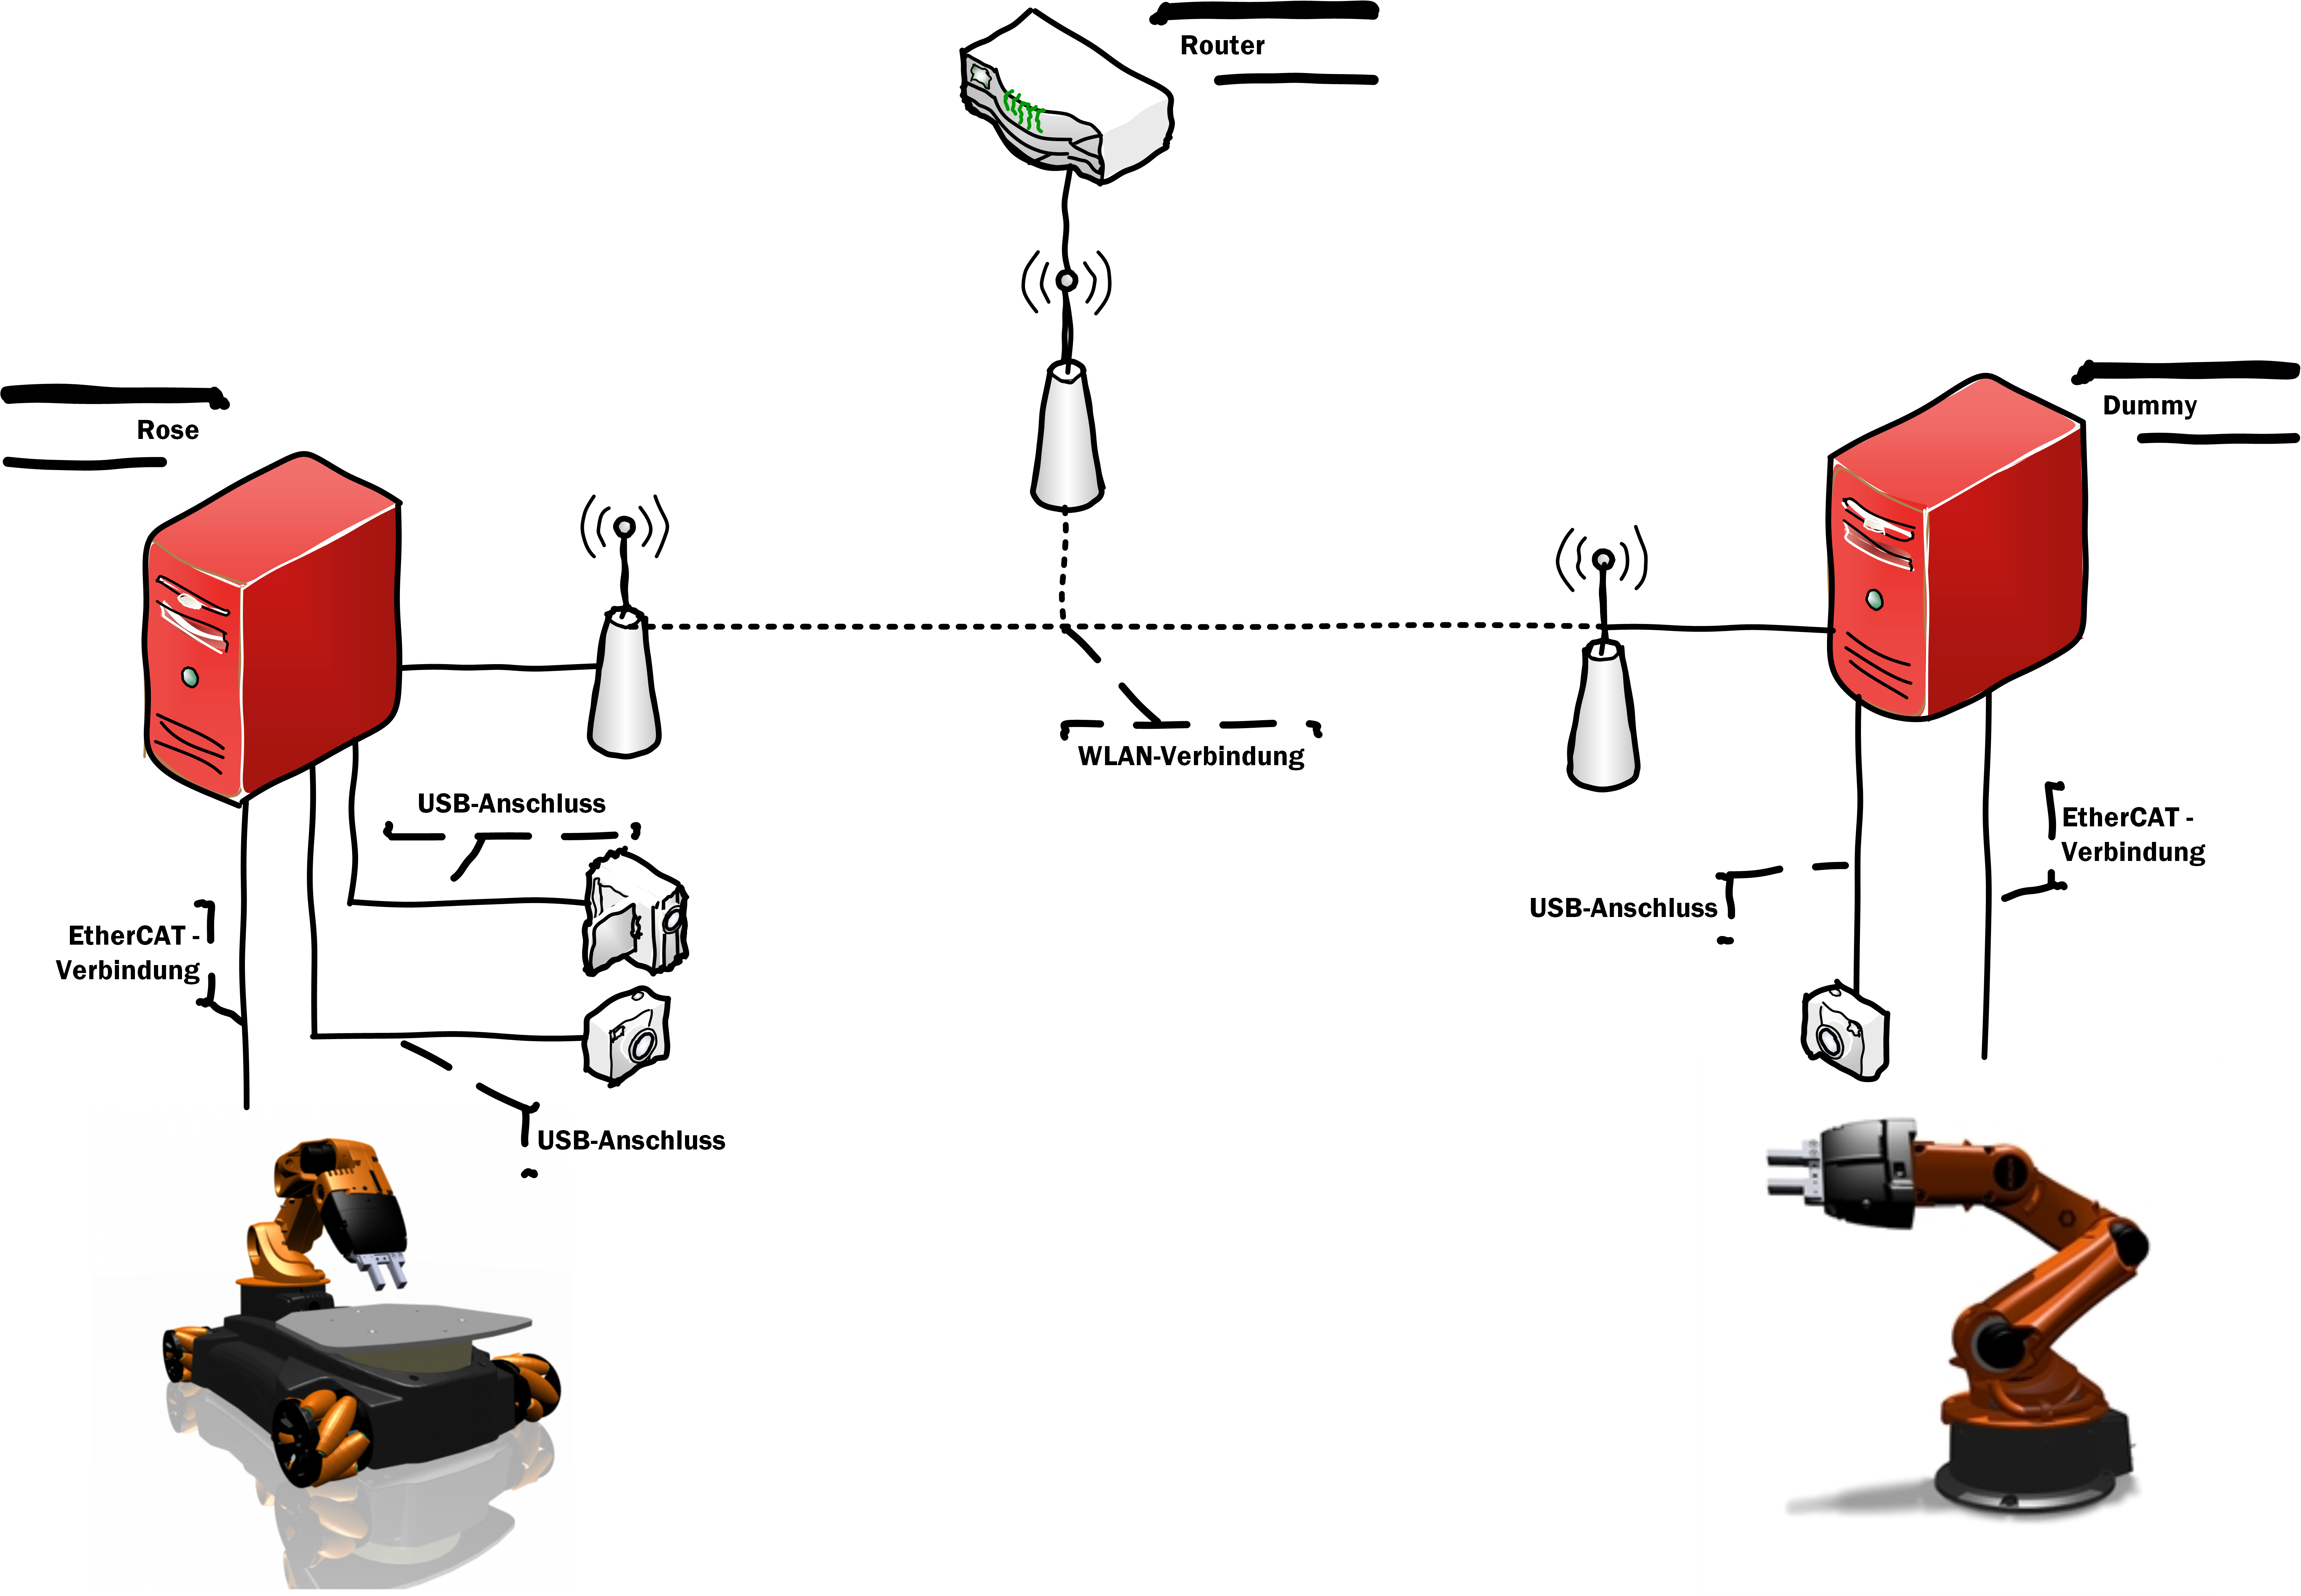
\includegraphics[scale=0.5]{fig/netw}   
	\caption[Schematische Darstellung der Verbindungen]{Schematische Darstellung der Verbindungen}
	\label{fig:aufbau-netw}
\end{figure}

Abbildung \ref{fig:aufbau-netw} stellt den genutzten Verbindungsplan dar. Die zentrale Komponente ist der Router, welcher mit einem externen Access-Point (AP) eine WLAN-Verbindung ermöglicht. Mit diesem WLAN verbinden sich die beiden Steuerungsrechner \textit{Rose} und \textit{Dummy}, welche beide unter diesen Hostnames im Netz erreichbar sind. Die Verbindungen auf beiden Seiten sind gleich gehalten. Die Verbindung zwischen Rechner und Roboter sind mit der EtherCAT-Schnittstelle (Ethernet for Control Automation Technology) realisiert. Diese Ethernet-Variante wurde für Echtzeit-Anforderungen entwickelt, indem Wert auf kurze Zykluszeiten ($\leq$ 100 $\mu$s) und  niedrigem Jitter für exakte Synchronisierung ($\leq$ 1 $\mu$s) gelegt wurde.\cite{ethercat} Die Verbindung zwischen den Rechnern und den Sensoren ist mit USB-Verbindungen umgesetzt. Dabei werden alle USB-Anschlüsse auf der mobilen Plattform von Rose vollständig durch die Sensoren, sowie dem WLAN-USB-Dongle und dem Tastatur/Maus-Dongle belegt. Weitere USB-Geräte sind nur durch einen zusätzlichen HUB möglich. 

Eine Alternative zu diesem Plan ist ein vermaschtes Netz, wie bei PEIS gefordet. Dadurch könnte der Router wegfallen, da alle Endgeräte direkt miteinander verbunden sind. Des Weiteren könnten einige Sensoren auf eigene Rechner ausgegliedert werden. Dies würde die einzelnen Rechner, besonders den leistungsschwachen Rechner von Rose, entlasten, aber auch die Netzwerkkomplexität und die Kosten steigern.\clearpage

%%%%%%%%%%%%%%%%%%%%%%%%%%%%%%%%%%%%%%%%%%%%%%%%%%%%%%%%%%%%%%%%%%%%%%%
%% Inhaltliche Kapitel
% TODO anpassen
%%%%%%%%%%%%%%%%%%%%%%%%%%%%%%%%%%%%%%%%%%%%%%%%%%%%%%%%%%%%%%%%%%%%%%%%
%% Inhaltliches Kapitel (Beispiel)
\section{Beispiel für Inhalte}
\label{sec:content}

Dieses Kapitel ist als Beispiel für die zu erstellenden Inhalte gedacht.



\subsection{Nutzung von Aufzählungen}
    \subsubsection{Einfache Aufzählungen}
        Einfache Aufzählungen erhält man über die \texttt{Itemize}-Umgebung:
        \begin{itemize}
        	\item erster Stichpunkt
        	\item zweiter Stichpunkt
            \begin{itemize}
            	\item erster verschachtelter Stichpunkt
            	\item noch einer
            	\begin{itemize}
            		\item Schachteln auf dritter Ebene
        		\end{itemize}
        	\end{itemize}
        	\item dritter Stichpunkt
        \end{itemize}
        
    \subsubsection{Nummerierte Aufzählungen}
        Aufzählungen lassen sich auch automatisch durchnummerieren mit der
        \texttt{Enumerate}-Umgebung:
        \begin{enumerate}
            \item erster Stichpunkt
            \item zweiter Stichpunkt
            \begin{itemize}
                \item erster verschachtelter Stichpunkt
                \item noch einer
                \begin{itemize}
                    \item Schachteln auf dritter Ebene
                \end{itemize}
            \end{itemize}
            \item dritter Stichpunkt
        \end{enumerate}
        
    \subsubsection{Definitions-Aufzählungen}
        Mit der \texttt{Description}-Umgebung lassen sich Definitions-artige Aufzählungen
        gestalten.
        \begin{description}
            \item[Begriff] und hier die längliche Beschreibung des tollen Begriffs,
            seiner Auswirkungen auf den Geisteszustand des Schreibers und die Folgen für
            den Leser
            \item[B2] noch ein Begriff
        \end{description}
    
    
    
\subsection{Tabellen und Bilder}
    \subsubsection{Einbinden von Abbildungen}
        Einfache Abbildungen lassen sich mit der \texttt{Figure}-Umgebung und dem
        \texttt{includegraphics}-Befehl einbinden:
        \begin{figure}
            \centering
            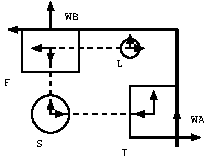
\includegraphics[scale=1.4]{fig/exampleSzene}   
            \caption{Typischer Beispieltext}
            \label{fig:beispielText}
        \end{figure}
            
        Abbildungen mit mehreren Teilabbildungen lassen sich über die
        \texttt{Subfigure}-Umgebung nutzen.
        \begin{figure}
            \centering
            \subfigure[teil 1]{%
                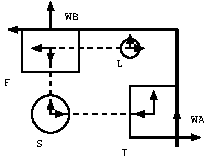
\includegraphics[scale=1]{fig/exampleSzene}
                \label{fig:beispielDepiktionenA}}
            \hfill
            \subfigure[teil 2]{%
                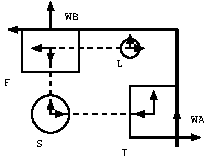
\includegraphics[scale=1]{fig/exampleSzene}
                \label{fig:beispielDepiktionenB}}
            \vfill
            \subfigure[teil 3]{%
                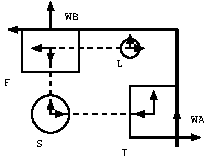
\includegraphics[scale=1]{fig/exampleSzene}
                \label{fig:beispielDepiktionenC}}
            \caption{Zum Beispieltext passende Abbildungen (Depiktionen)}
            \label{fig:beispielDepiktionen}
        \end{figure}
        
        Als Quellen eigenen sich PDF- und JPG-Dateien. Andere Dateien müssen vor der
        Benutzung konvertiert werden.
    
    
    \subsubsection{Tabellen}
        Tabellen gehen in der \texttt{Table}-Umgebung mit Hilfe des \texttt{tabular}-Befehls.
        \begin{table}
            \centering
            \begin{tabular}{l|l||r}
                \multicolumn{2}{l}{zwei Spalten zusammengefasst} & dritte Spalte\\
                Spalte 1 & Spalte 2 & Spalte 3 \\\hline\hline
                Spalte 1 & Spalte 2 & Spalte 3 \\\hline
                Spalte 1 & Spalte 2 & Spalte 3 \\\hline
            \end{tabular}
            \caption{Beispieltabelle}
            \label{tab:beispieltabelle}
        \end{table}
        
        Ansonsten funktioniert die Umgebung änhlich wie die
        \texttt{Figure}-Umgebung.
    
    
    \subsubsection{Quellcode}
        Quellcode lässt sich mit Hilfe des \texttt{Listings}-Paketes einbinden.
        Sinnvollerweise definiert man sich dazu in der Präambel des
        Hauptdokuments eine passende neue \texttt{lstnewenvironment}-Umgebung, die man
        dann einfach nutzen kann und die neben Snytax-Highlighting auch andere
        Dinge wie Rahmen, Zeilennummern, Bildunter- oder überschriften
        etc.~beherrscht.
        
        \begin{figure}
        \centering
        \begin{java}
public class Student {
    private String name;

    public Student(String name) {
        this.name = name; 
    }
    
    public static void main(String[] args) {
        Student s = new Student();
    }
}
        \end{java}
        \caption{Sourcecode für Kram}
        \label{fig:source}
        \end{figure}
        
        
     \subsubsection{Quellcode}
        Algorithmen schreibt man entweder als Pseudocode (über das
        \texttt{Listings}-Paket) oder aber mit Hilfe der \texttt{algorithm}-Umgebung aus
        dem Paket \texttt{algorithm2e}
        
        \begin{center}
        \begin{algorithm}[ht]
        \DontPrintSemicolon
        \LinesNumbered
        \SetKwFunction{init}{init}
        \SetKwFunction{evaluate}{evaluate}
        \SetKwFunction{recombine}{recombine}
        \SetKwFunction{mutate}{mutate}
        \SetKwFunction{select}{select}
        \SetKw{nicht}{not}
        \SetKw{und}{and}
        \Begin{
            $t$ = 0\;
            \init{$P(t)$}\;
            \evaluate{$P(t)$}\;
            \While{\nicht optimal \und \nicht Abbruch}{
                $PP(t) = $ \recombine{$P(t)$}\;
                \mutate{$PP(t)$}\;
                \evaluate{$PP(t)$}\;
                $P(t+1) = $ \select{$PP(t)$, $P(t)$}\;
                $t = t+1$\;
            }
        }
        \caption{Ablauf eines hybriden EA}
        \label{alg:eaHybrid}
        \end{algorithm}
        \end{center}
        

    
\subsection{Referenzierungen}
    \subsubsection{Zitate}
    Zitieren geht mit dem Befehl \texttt{cite}: \cite{Claus98a} bzw. mit den Befehl
    \texttt{citep}: \citep{wagner2009tele}. Als Argument
    benötigt man den Schlüssel für die jeweilige Referenz, so wie er in der
    .bib-Datei hinterlegt ist bzw.~durch Tools wie JabRef generiert wird. 
    
    Wenn man etwas nicht direkt zitieren möchte, aber die Literaturquelle im
    Literaturverzeichnis erscheinen soll, dann nutzt man den Befehl
    \texttt{nocite}.
    
    \subsubsection{Querverweise}
    Den Anker für die Querverweise setzt man mit dem Befehl \texttt{label}.
    Bezugnehmen kann man dann mit Hilfe von \texttt{ref} oder \texttt{pageref},
    wobei ersteres durch die entsprechende Gliederungsnummer (Überschrift,
    Abbildung, Tabelle, \ldots) ersetzt wird und letzteres durch die
    Seitennummer, auf der der Anker für die Referenz gesetzt wurde.
    Beispiel: Abbildung \ref{fig:beispielText} erscheint auf Seite
    \pageref{fig:beispielText}.
    
    
\subsection{Fussnoten}
    Fussnoten setzt man mit Hilfe des Befehls \texttt{footnote}. Dieser folgt
    entweder direkt auf das Wort, welches man mit einer Fussnote versehen möchte
    oder aber auf das Satzendezeichen, wenn man einen ganzen Satz/Absatz meint.
    Beispiel:\footnote{Das ist meine erste Fussnote.}
    
    
\subsection{Mathe}
Für Mathe siehe \href{http://www.ams.org/tex/short-math-guide.html}{{\tt
www.ams.org/tex/short-math-guide.html}}.


    
    
    
\clearpage
%%%%%%%%%%%%%%%%%%%%%%%%%%%%%%%%%%%%%%%%%%%%%%%%%%%%%%%%%%%%%%%%%%%%%%%

%%%%%%%%%%%%%%%%%%%%%%%%%%%%%%%%%%%%%%%%%%%%%%%%%%%%%%%%%%%%%%%%%%%%%%%
%% Zusammenfassung und Ausblick
\section{Entwicklung}
\label{sec:entwicklung}
Dieses Kapitel befasst sich mit einzelnen Aspekten der Entwicklung. Nach der Auflistung der Nicht-funktionalen Anforderungen, sowie der Funktionen, werden grundlegende Konzepte und Architekturen vorgestellt. Dabei werden erste Sensoren, Aktoren und bestehende Software Bibliotheken getestet und für eine Anschlussverwendung bewertet. Die weiteren benötigten Softwarepaket werden im nachfolgenden Kapitel Implementierung TODO umgesetzt.

\subsection{Nicht-Funktionale Anforderungen}
\label{sec:dev-nichtfunk}

Die nicht-funktionalen Anforderungen beschreiben Qualitätsmerkmale des MRS. Diese sind in verschiedene Kategorien gruppiert und haben Auswirkungen auf die Funktionalität und die Architektur. Im Folgenden werden nur die für diese Arbeit relevanten Kategorien erläutert und in Bezug gebracht.

\subsubsection{Sicherheit - Safety}

Im englischen wird der Begriff Sicherheit in die Terme \textit{Security} und \textit{Safety} unterteilt. Ersteres beschäftigt sich unter anderem mit der Verschlüsselung von Daten. Der Begriff \textit{Safety} bezieht sich auf die Anwendersicherheit, zum Beispiel ob dieser durch das System Verletzungen erleiden kann oder ob sich das System selbst oder die Umwelt beschädigt. Da die Roboter in dieser Arbeit nicht, wie Industrieroboter, durch Gitterzäune gesichert sind wird eine Lichtwarnanlage installiert. Diese arbeitet ähnlich einer Ampel. Befindet sich das System in einer sicheren Stellung, in der es sich nicht bewegt, leuchtet die Lichtanlage in grün. Wird eine Bewegung geplant oder ist das System vor einer Bewegung blinkt die Lichtanlage fünf Sekunden gelb. Innerhalb dieses Intervalls bewegt sich das System nicht. Auf das Blinken folgt ein rotes Leuchten der Lichtanlage. In dieser Zeit führen die Roboter ihre Aktionen aus. Während dieser Aktionen nutzt das Robotersystem die Sensoren und berechnet kollisionsfreie Pfade um nicht mit sich selbst oder der Umwelt zu kollidieren. Objekte, die sich erst zur Laufzeit auf dem Pfad befinden, werden in dieser Arbeit noch nicht beachtet und können so zur Kollision führen. Um bei Bewegungen der mobilen Plattform oder zwischen zwei Tasks der Arme die Sicherheit dieser zu sicheren existieren die beiden Posen \textit{Candle} und \textit{Fold}. Die erste Pose streckt den Arm senkrecht in die Höhe und ermöglicht so kollisionsfreie Pfade in die meisten anderen Posen. In der zweiten Pose befinden sich alle Gelenke in ihrer minimalen Konfiguration. Sollte dem Roboter der Strom fehlen, bedingt durch einen Stromausfall oder leere Batterien, fällt der Roboterarm in sich zusammen, da die Gelenkmotoren die Position nicht mehr halten können. In der \textit{Fold}-Pose kann der Roboter nicht weiter in sich zusammenfallen, da alle Glieder aufeinander liegen. Deshalb sollten die Roboter diese Pose in längeren Inaktivitätsphasen einnehmen. Diese Aspekte werden während der Entwicklung der Funktionen berücksichtigt.

\subsubsection{Zuverlässigkeit}
Die Zuverlässigkeit des Systems beschreibt unter anderem das Systemverhalten bei einem Fehlerfall oder Teilsystemausfall. Das Robotersystem darf dabei nicht in einen unsicheren Zustand geraten. Da das Robotersystem auf ROS aufbaut werden einzelne Aktoren und Sensoren als ROS-Node betrieben. Jeder Node stellt dabei ein einzelnes Subsystem dar, welcher ausfallen kann. ROS ist so konzipiert, dass das ganze System nicht abstürzt, wenn ein einzelner Node ausfällt. Eine Schwachstelle bildet hierbei der ROS-Core. Dieser stellt den Mittelpunkt eines ROS-Systems dar. Fällt dieser aus bricht die Kommunikation zwischen den einzelnen Nodes zusammen. In diesem Fall müssen die Nodes in einen sicheren Fehlerzustand übergehen. Dies betrifft vor allem die Aktoren, besonders die Steuerungen der Roboter. 

Ein weiterer Aspekt der Zuverlässigkeit ist die Wiederherstellbarkeit. Dies betrifft ob und wie komplex ein bestimmter fehlerfreier Systemstatus wiederhergestellt werden kann. Da die Nodes einzelne Subsysteme sind, können diese nach einem Ausfall einfach wieder gestartet werden und der Systemstatus ist wiederhergestellt. Dies betrifft auch den ROS-Core. Wird dieser auf der selben Adresse (IP und Port) neu gestartet, nehmen alle Nodes die Kommunikation wieder auf. Diese beiden Aspekte werden vor allem bei der Entwicklung der Architektur für das MRS berücksichtigt. Dabei ist das zentrale Koordinierungs- und Konfigurations-System eine Komponente, die zu einem potenziellen Single-Point-of-Failure führen kann.


\subsubsection{Korrektheit}
Die Korrektheit lässt sich in dieser Entwicklung durch die Genauigkeit der Funktionen definieren. So dürfen die Positionen und Orientierungen der Arme und der mobilen Plattform nur um bestimmte Grenzen abweichen. Dabei gelten für die End-Effektor-Pose eine Distanzabweichung von maximal 5mm für jede Dimension und für die Orientierung eine Abweichung von maximal 1\textdegree pro Achse. Dies muss bei der Entwicklung der inversen Kinematik berücksichtigt werden. Für die mobile Plattform gelten andere maximale Abweichungen. Für die Distanzabweichungen sind das 5cm in X- und Y-Richtung. Für die Z-Dimension darf sie maximal 5mm sein. Für die Rotation gilt: Z-Achse 5\textdegree, X- und Y- Achse 1\textdegree.

\subsubsection{Leistung}
Die Leistung bezieht sich auf die Effizienz des MRS. Besonders der Zeit- und Energieaufwand sollen möglichst minimiert werden. Der Zeitaufwand bezieht sich dabei nicht auf die Performance-Optimierung der Algorithmen, sondern der Bewegungen und deren Abläufe. Dieser Aspekt muss bei der Entwicklung der Funktionen und der Implementierung berücksichtigt werden. Der Energieaufwand ist stark abhängig von den benutzten Aktoren und wird bei der Entwicklung der inversen Kinematik für die Arme und die Pfadbestimmung für die mobile Plattform in Betracht gezogen.

\subsubsection{Änderbarkeit}
Die Änderbarkeit besteht aus Sicht der Entwicklung aus mehreren Aspekten. Für diese Arbeit ist dabei die Erweiterbarkeit ein wichtiger Aspekt. Zum einen geht es um die Erweiterbarkeit des MRS um weitere Sensoren und Aktoren. Diese sollen möglichst einfach in das bestehende MRS eingebunden werden können ohne bestehende Subsysteme zu verändern. Zum anderen soll in der Weiterentwicklung dieses MRS weitere Konzepte eingebunden werden. So müssen für eine automatische Konfiguration und verteilte Koordinierung Schnittstellen in der Architektur entworfen werfen. Diese Schnittstellen sollen unter anderem eine Markt-basierte Konfiguration ermöglichen. Diese beiden Aspekte der Erweiterbarkeit müssen in der Entwicklung der Architektur und der Funktionen berücksichtigt werden. So sind grobe Kostenangaben für die Funktionen ein möglicher Ansatz für die Gebote am Markt.

\subsection{Funktionalitäten}
\label{sec:dev-funk}

In diesem Kapitel werden die Funktionen des Robotersystem aufgelistet. Das folgende Use-Case Diagramm \ref{fig:dev-usecase} stellt die groben Funktionsanforderungen an das Robotersystem dar.

\begin{figure}[H]
	\centering
	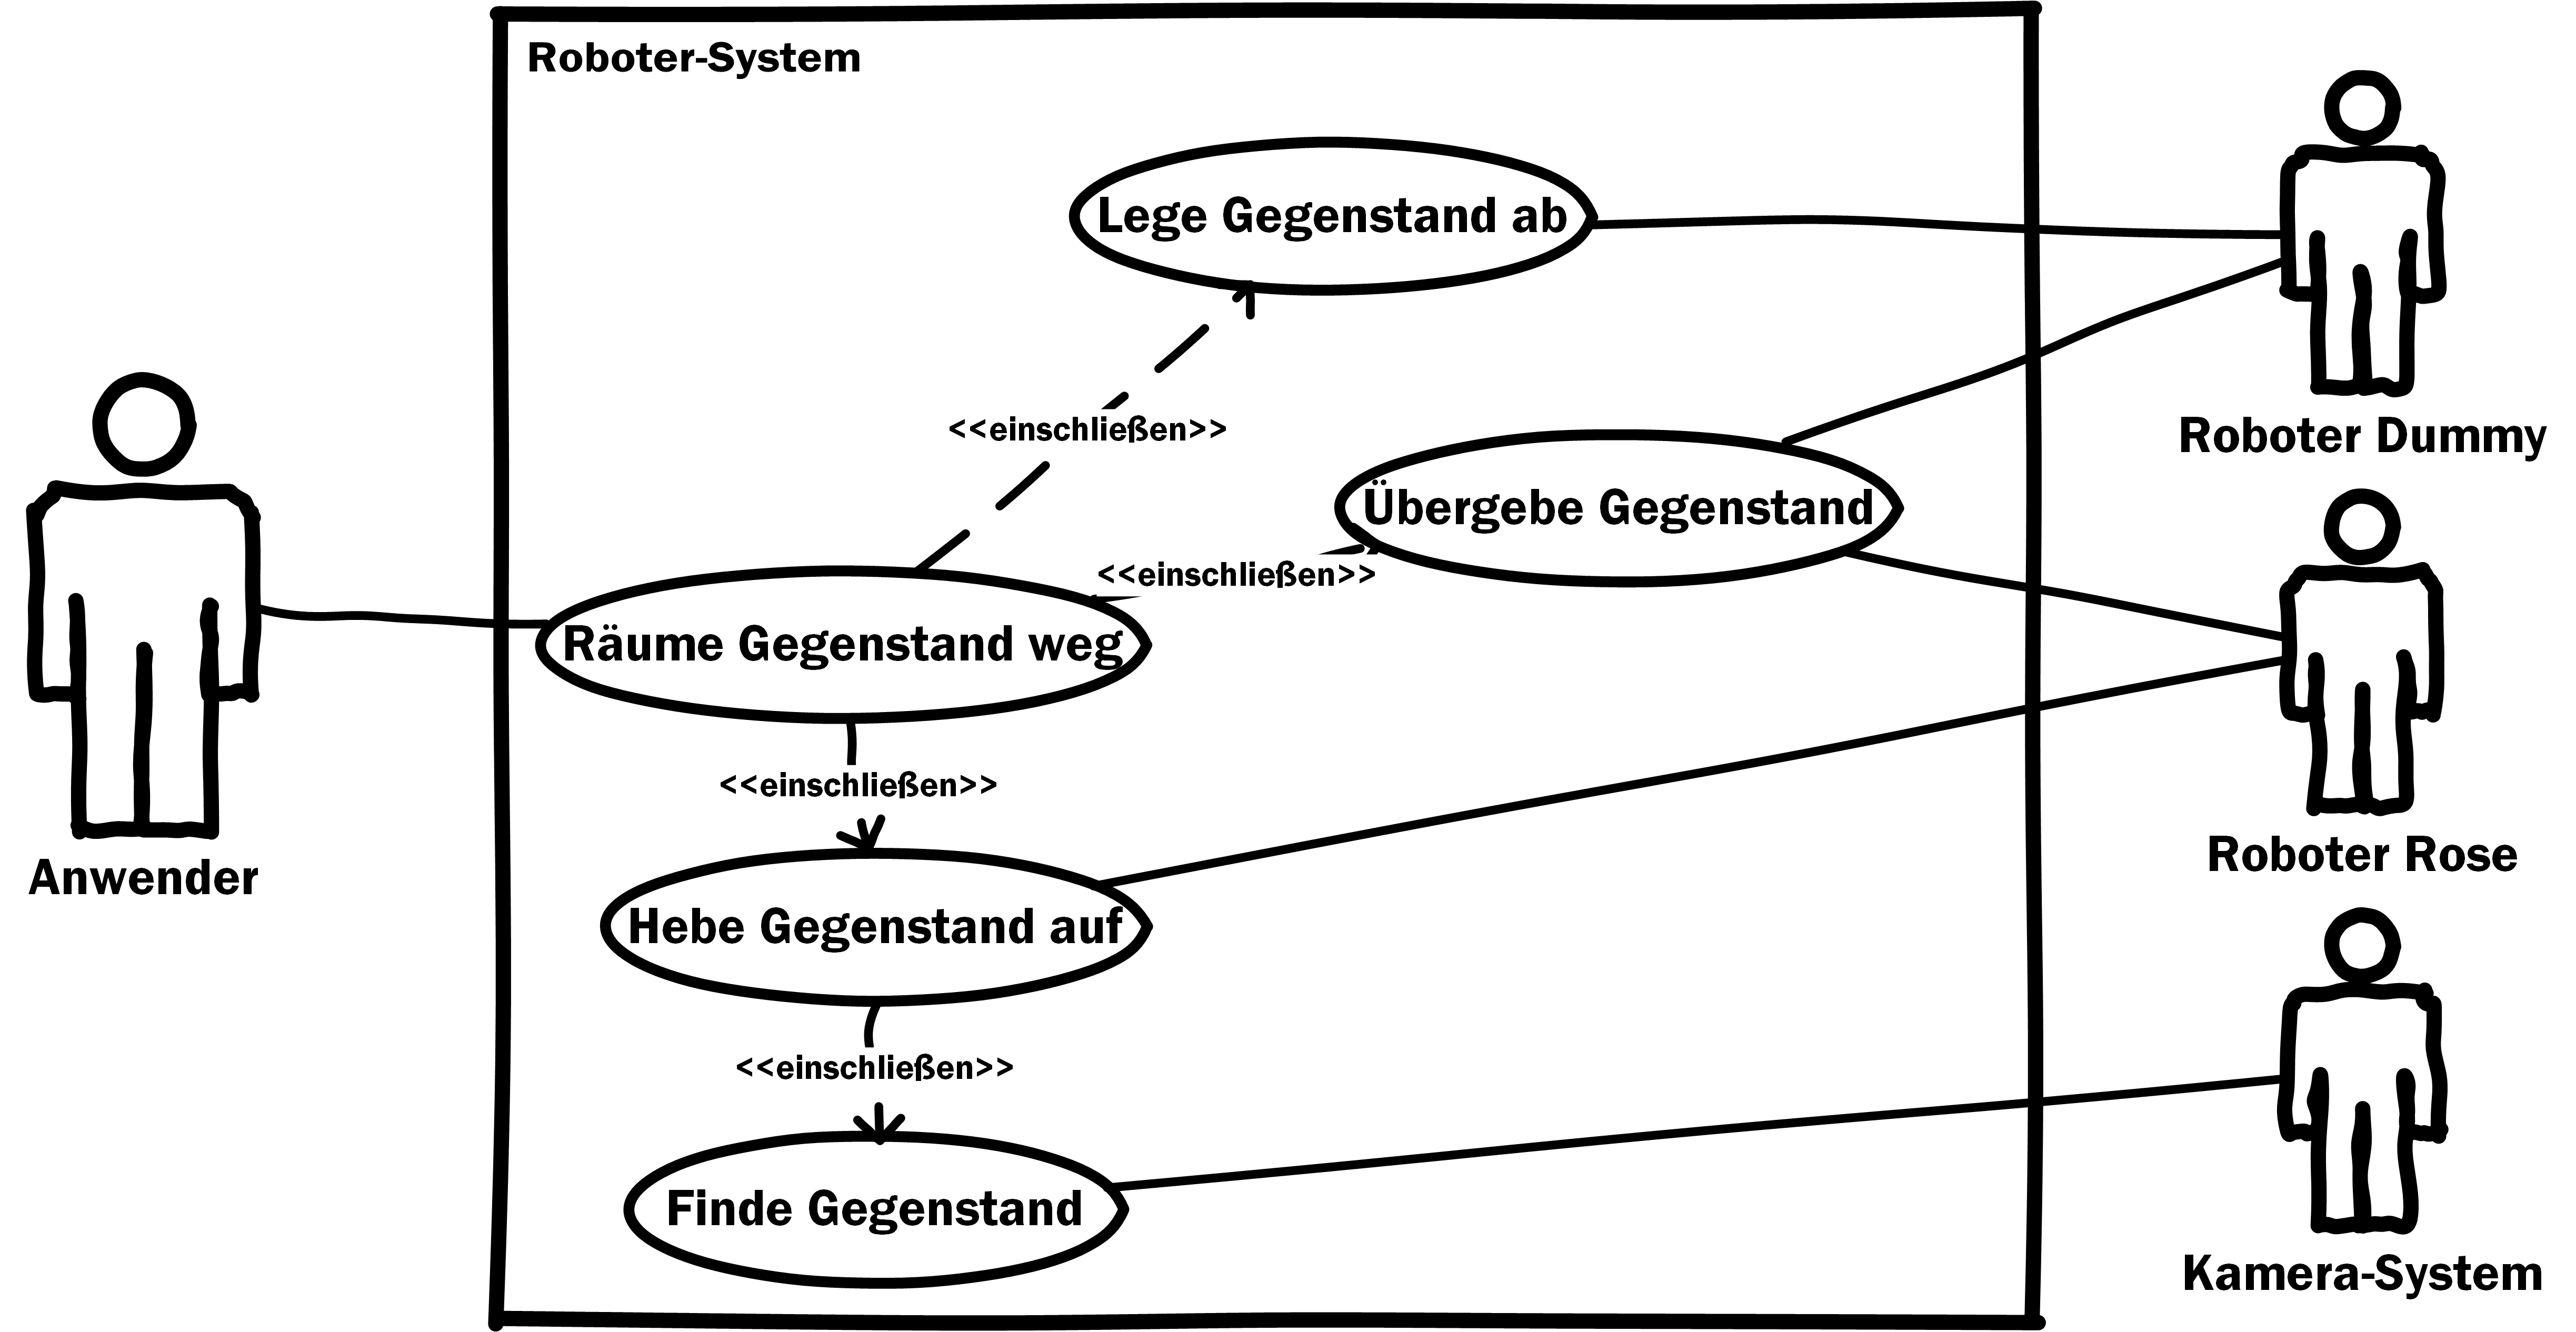
\includegraphics[scale=0.8]{fig/UseCase}   
	\caption[Use-Case Robotersystem]{Vereinfachtes Use-Case Diagramm zur groben Funktionsübersicht des Robotersystems}
	\label{fig:dev-usecase}
\end{figure}

Der Anwender gibt dem System die Anweisung einen Gegenstand wegzuräumen. Das Robotersystem gliedert die Anweisung in einzelne Tasks auf. Diese Tasks werden von den unterschiedlichen Akteuren mit ihren Funktionalitäten sequentiell oder parallel ausgeführt. In diesem konkreten Fall soll zunächst der Roboter Rose den entsprechenden Gegenstand aufheben. Dies erfordert zunächst eine Lokalisierung des Objektes die von einem Kamerasystem angefordert wird. Anschließend übergeben sich die Roboter Rose und Dummy den Gegenstand, bevor Dummy ihn anschließend an einer gewünschten Position ablegt. Diese sehr grobe Darstellung des Vorgangs beinhaltet die vier zentralen Funktionen, die das System umsetzen muss: Gegenstand aufheben (\textit{pick-up}), Gegenstand ablegen (\textit{place}), Gegenstand lokalisieren und Gegenstand übergeben(\textit{handover}).

 Die folgenden Anforderungen dienen zur Strukturierung der Arbeit und zerlegen das Robotersystem in Teilsysteme. Dies wird benötigt um einen Aufwand für die Koordinierung und Konfiguration zu bestimmen. Deshalb sind die Anforderungen grobe Darstellungen und aus dem Aspekt der Software-Entwicklung nicht detailliert genug. Dafür müssten die Funktionen weiter runter gebrochen werden. Dies würde jedoch den Umfang dieser wissenschaftlichen Arbeit überschreiten.

Alle Funktionen werden nach dem Schema aus \cite{lundh2006plan} angegeben: 

$f = \langle  Id, r, I, O, \Phi, Pr, Po, Freq, Cost\rangle$

Jede Funktion $f$ entspricht dabei einem Tupel und ist einem oder mehreren Agenten im System zugewiesen. Diese Zuweisung wird im Feld $r$ in Kapitel TODO zugewiesen. Die weiteren Felder des Tupels stehen für:

\begin{description}
	\item [$Id$] Eindeutiger Bezeichner für die Funktion.
	\item [$I = \{i_1, i_2,\ldots,i_n\}$] Eine Menge aller Eingangsparameter.
	\item [$O = \{o_1, o_2,\ldots,o_n\}$] Eine Menge aller Ausgangsparameter.
	\item[$\Phi$] Definiert den Übergang zwischen Eingabe und Ausgabe.
	\item [$Pr$] Zustand $s \in S$ aus dem diese Funktion gestartet werden kann.
	\item [$Po : S \times I \rightarrow S$] Eine Funktion die den Folgezustand $s\textasciiacute$ anhand des Inputs und des Startzustandes $s$ angibt.
	\item[$Freq$] Frequenz in der die Funktionalität ausgeführt werden soll.
	\item[$Cost$] Kosten der Ausführung, zum Beispiel Zeit oder Energie. Können konstant aber auch funktionell angegeben werden.
\end{description}

Je nach Typ des Agenten sind die Eingabemenge bei Sensoren $I = \varnothing$ und die Ausgabemenge bei Aktoren $O =  \varnothing$. Außerdem wird jede Funktion beschrieben und für die Verwendung in ein MRS eingeordnet. Aus dem Anwendungsfall für das Robotersystem ergeben sich folgende funktionale Anforderungen.

\subsubsection{Funktion Aufheben}

\begin{tabular}{|p{3cm}|p{10cm}|}
	\multicolumn{2}{c}{	$f_0$ (Aufheben):}\\
	\hline  $Id$ & pickup\\ 
	\hline  $I$ & Objektposition im globalen oder lokalen Koordinatensystem. \\ 
	\hline  $O$ & Erfolgsmeldung. \\ 
	\hline  $\Phi$ & Wenn die Objektposition durch den Agenten erreichbar und der Agent voll funktionsfähig ist erfolgt eine positive Rückmeldung. Ansonsten eine negative Erfolgsmeldung.\\ 
	\hline $Pr$ & Zustand $s_1$, Objekt im Nahfeld gefunden und Arm in Candle-Stellung. \\ 
	\hline $Po$ & Zustand $s_2$, Arm in Candle-Stellung und Objekt gegriffen, oder Fehlerzustand $s_e$ bei Fehlschlag. \\ 
	\hline $Freq$ & Einmalige Funktion. \\ 
	\hline $Cost$ & Dynamisch zu ermitteln. Abhängig von Weg und Erreichbarkeit des Objektes. \\
	\hline
\end{tabular}

\paragraph{Beschreibung}
Die Funktion \textit{pickup} wird in den beiden Robotern Rose und Dummy implementiert und wird für das Aufheben von Objekten genutzt. Beschränkt wird diese Funktionalität durch die Erreichbarkeit der Objektposition. Gerade für den stationären Dummy ist der Arbeitsraum stark eingeschränkt. Rose hat die Möglichkeit während dieser Funktionalität die eigene Position zu verändern um das Objekt zu erreichen. Das Aufheben bedingt, dass das Objekt auf einer parallelen Ebenen zur X-Y-Ebene liegt, da die Greifer Z-Achse parallel zur globalen Z-Achse greift. Die Rotation um die Z-Achse des Objektes ist dabei frei wählbar, da diese durch eine Rotation des Greifers ausgeglichen werden kann. Damit der Roboter nicht auf dem Weg zum Objekt dasselbe berührt wird eine Position über dem Objekt angefahren, bevor der Greifer an der globalen Z-Achse hin abfährt.  Diese Beschränkung reduziert die Arbeitsräume der Roboterarme, da ein senkrechter Griff die Zahl der möglichen Gelenkpositionen stark einschränkt und jede Position auf dem senkrechten Pfad erreichbar sein muss. Eine nicht erreichbare Position führt zum Abbruch der Funktion. Eine anschließende sichere Konfiguration des Roboterarms ist nicht gewährleistet. Für Rose gilt des Weiteren auch ein undefinierter Standort nach Abbruch. Wird die Funktion erfolgreich beendet befindet sich der Arm in einer sicheren Konfiguration (\textit{Candle}- oder \textit{Fold}-Pose).

\paragraph{Einordnung}
Die Funktion ist als Single-Robot Task für einen Single-Task-fähigen Agenten einzuordnen, da nur ein Agent zur Erledigung nötig ist. Die Funktion kann von einem Multi-Task fähigen Agenten intern auch parallel ausgeführt werden, da einzelne Subtasks unabhängig von einander erledigt werden können. Ein Beispiel ist das Öffnen des Greifers während der Bewegungsphase des restlichen Armes oder der mobilen Plattform bei Rose. Diese Multi-Task Anwendung fordert aber einen höheren Koordinierungsaufwand, da Funktionen zeitlich voneinander abhängen (siehe TODO). Für eine Single-Task Anwendung ist der Koordinierungsaufwand gering, da alle Subtasks seriell ausgeführt werden. Der Konfigurationsaufwand ist mittel, da zwei Agenten für die Funktionalität bereitstehen, welche sich über den Aktionsradius für die Ausführung qualifizieren. 

\subsubsection{Funktion Ablegen}

\begin{tabular}{|p{3cm}|p{10cm}|}
	\multicolumn{2}{c}{$f_1$ (Ablegen):}\\
	\hline  $Id$ & place\\ 
	\hline  $I$ & Zielposition im globalen oder lokalen Koordinatensystem. \\ 
	\hline  $O$ & Erfolgsmeldung. \\ 
	\hline  $\Phi$ & Wenn die Zielposition durch den Agenten erreichbar und der Agent voll funktionsfähig ist erfolgt eine positive Rückmeldung. Ansonsten eine negative Erfolgsmeldung.\\ 
	\hline $Pr$ & Zustand $s_2$, Arm in Candle-Stellung und Objekt gegriffen. \\ 
	\hline $Po$ & Ruhezustand $s_r$, Arm in Candle-Stellung oder Fehlerzustand $s_e$ bei Fehlschlag. \\ 
	\hline $Freq$ & Einmalige Funktion.\\ 
	\hline $Cost$ & Dynamisch zu ermitteln. Abhängig von Weg und Erreichbarkeit der Zielpositionen. \\
	\hline
\end{tabular}

\paragraph{Beschreibung}
Ähnlich Funktion $f_0$ wird diese Funktionalität den beiden Robotern Dummy und Rose implementiert. Dabei legt der Arm ein Objekt an einer gewünschten Position ab. Beschränkt wird die Funktion auch durch den Arbeitsraum der einzelnen Roboter.  Das Objekt kann ebenfalls nur auf einer Ebene abgelegt werden, die parallel zur X-Y-Ebene ist. Die Rotation um die Z-Achse kann beim ablegen vorgegeben werden. im Gegensatz zu $f_0$ nähert sich der Greifer nicht dem Objekt an, sondern entfernt sich nach dem Ablegen positiv auf der globalen Z-Achse vom Objekt um dieses in einer anschließenden Bewegung nicht durch eine Berührung zu manipulieren. Bei einer erfolgreichen Ausführung beendet die Funktionalität befindet sich der Arm in einer sicheren Konfiguration (\textit{Candle}- oder \textit{Fold}-Pose). Bei einem Fehlschlag ist diese Konfiguration nicht garantiert.

\paragraph{Einordnung}
Die Funktion gilt als Single-Robot Task. Die Subtasks der Funktion können seriell als auch parallel ausgeführt werden. Dadurch eignen sie sich für Multi-Task, sowie Single-Task Agenten. Je nach Typ ist der Koordinierungsaufwand unterschiedlich hoch. Der Single-Task Agent benötigt wenig Koordinierung da nur ein Startsignal notwendig ist. Bei einem Multi-Task Agenten ist die Koordinierung aufwendiger, da Subtasks zeitlich voneinander abhängen. Zum Beispiel darf der Greifer erst öffnen, wenn das Objekt in der Position ist. Der Konfigurationsaufwand ist gering, da nur der Agent die Aktion ausführen kann, der den Gegenstand hält. 

\subsubsection{Funktion Objekt identifizieren und lokalisieren}
\label{sec:funraum}

\begin{tabular}{|p{3cm}|p{10cm}|}
	\multicolumn{2}{c}{$f_2$ (Objekt im Raum finden):}\\
	\hline  $Id$ & findObj\\ 
	\hline  $I$ & Gewünschte Objektdaten. \\ 
	\hline  $O$ & Position des Zielobjektes im globalen Koordinatensystem. \\ 
	\hline  $\Phi$ & Findet der Agent anhand der Objektdaten das Objekt wird die Position zurückgegeben. Ansonsten folgt eine Fehlermeldung.\\ 
	\hline $Pr$ & Ruhezustand $s_r$,Keine Vorbedingung nötig. \\ 
	\hline $Po$ & Zustand $s_0$, Objekt gefunden. Oder Fehlerzustand $s_e$\\ 
	\hline $Freq$ & Einmalige Funktion.\\ 
	\hline $Cost$ & Konstant. Abhängig von Prozessor der Recheneinheit, Algorithmus und Kamerasystem. \\
	\hline
\end{tabular} 

\paragraph{Beschreibung}
Diese Funktion identifiziert und lokalisiert ein bestimmtes Objekt im Großraum (Bodenfläche im Arbeitsraum größer als ein Quadratmeter). Je nach Typ der Identifizierung werden unterschiedliche Objektdaten benötigt. Eine Identifizierung basierend auf der Farbe des Objektes benötigt die Objektfarbe. Eine Identifizierung basierend auf der Form benötigt ein 3D-Modell oder eine Kostenfunktion für das Objekt. Die Identifizierung ist abhängig vom verwendeten Algorithmus. Dieser wird in TODO genauer erklärt. Findet die Funktion das gewünschte Objekt nicht oder tritt ein Fehler bei der Erkennung auf bricht die Funktion ab und gibt eine Fehlermeldung zurück. Bei einer erfolgreichen Identifizierung wird anhand von 3D-Daten die Position des Objektes berechnet. Bei dieser Lokalisierung soll eine Genauigkeit von fünf cm erreicht werden und damit nur eine grobe Position. Genauere Ergebnisse werden mit der Naherkennung $f_3$ erreicht. 

\paragraph{Einordnung}
Ein simpler Single-Robot Task, der von einem Agenten ausgeführt wird. Der Task wird in zwei Subtasks (Identifizieren und Lokalisieren) zerlegt, die serielle ausgeführt werden. Damit bringen Multi-Task Agenten keinen Vorteil. Der Koordinierungsaufwand ist sehr gering, da die Funktion nur angestoßen werden muss. Sollte die Funktion jedoch mit mehreren Kamerasystemen genutzt werden steigt der Koordinierungsaufwand, da der Task entweder parallel oder seriell von allen Systemen ausgeführt werden kann. Je nach Typ steigt der Konfigurationsaufwand, bei einer parallelen Ausführung ist kein Aufwand nötig, da immer alle Kamerasysteme genutzt werden. Eine serielle Ausführung würde die Komplexität steigen, da die Kamerasysteme in einer, möglicherweise priorisierten, Reihenfolge angestoßen werden.

\subsubsection{Funktion Nahfeld Erkennung}
\label{sec:funnah}

\begin{tabular}{|p{3cm}|p{10cm}|}
	\multicolumn{2}{c}{$f_3$ (Nahfeld Erkennung):}\\
	\hline  $Id$ & findObjNear\\ 
	\hline  $I$ & Gewünschte Objektdaten. \\ 
	\hline  $O$ & Position des Zielobjektes im lokalen Koordinatensystem. \\ 
	\hline  $\Phi$ & Findet der Agent anhand der Objektdaten das Objekt wird die Position zurückgegeben. Ansonsten folgt eine Fehlermeldung.\\ 
	\hline $Pr$ & Zustand $s_0$, Objekt im Raum gefunden und im Arbeitsraum der Kamera. \\ 
	\hline $Po$ & Zustand $s_1$, Objekt im Nahfeld gefunden. Oder Fehlerzustand $s_e$\\ 
	\hline $Freq$ & Einmalige Funktion.\\ 
	\hline $Cost$ & Konstant. Abhängig von Prozessor der Recheneinheit, Algorithmus und Kamerasystem. \\
	\hline
\end{tabular} 

\paragraph{Beschreibung}
Diese Funktion identifiziert und lokalisiert ein bestimmtes Objekt im Nahfeld (Bodenfläche im Arbeitsraum kleiner als ein Quadratmeter). Es gelten die gleichen Merkmale wie bei $f_2$. Der verwendete Algorithmus wird in TODO genauer erklärt. Findet die Funktion das gewünschte Objekt nicht oder tritt ein Fehler bei der Erkennung auf bricht die Funktion ab und gibt eine Fehlermeldung zurück. Zusätzlich zur Position wird auch die Orientierung des Objektes berechnet. Die bestimmte Position entspricht dem Flächenschwerpunkt der Oberfläche des Objektes und soll eine Genauigkeit von fünf mm entsprechen.

\paragraph{Einordnung}
Wie $f_2$ einzuordnen. Kann jedoch nicht mit mehreren Kamerasystemen ausgeführt werden, da jedes Kamerasystem auf einem Roboter montiert und mit diesem eng-gekoppelt ist. Dadurch ist der Konfigurationsaufwand konstant, da jedem Roboter ein System zugewiesen wird. 

\subsubsection{Funktion Agentenlokalisierung}
\ref{sec:funl}
\begin{tabular}{|p{3cm}|p{10cm}|}
	\multicolumn{2}{c}{$f_4$ (Lokalisierung Agent):}\\
	\hline  $Id$ & loc\\ 
	\hline  $I$ & $\emptyset$ \\ 
	\hline  $O$ & Position des Agenten im globalen Koordinatensystem. \\ 
	\hline  $\Phi$ & Kann der Agent sich selbst im Raum lokalisieren, wird die Position zurückgegeben. Ansonsten folgt eine Fehlermeldung.\\ 
	\hline $Pr$ & In jedem Zustand $s_s$ möglich \\ 
	\hline $Po$ & Wie der Zustand beim Start $s_s$.\\ 
	\hline $Freq$ & Abhängig vom Sensor.\\ 
	\hline $Cost$ & Konstant. Abhängig von Prozessor der Recheneinheit, Algorithmus und Kamerasystem. \\
	\hline
\end{tabular} 

\paragraph{Beschreibung}
Diese Funktionalität lokalisiert den entsprechenden Agenten im Raum. Mögliche Algorithmen sind das Nutzen der Odometrie-Daten, bildbasierte Odometrie, bildbasierte Lokalisierung beruhend auf externen Sensoren und Funktionen ($f_2$) oder bildbasierte Lokalisierung basierend auf Merkmals-Erkennung. Es existieren noch weitere Methoden der Lokalisierung, dafür fehlen aber in dieser Arbeit die entsprechenden Sensoren und Aktoren.

\paragraph{Einordnung}
Eine an den Agenten enge-gekoppelte Funktionalität die an einen mobilen Roboter oder externen Sensor vergeben werden kann. Ein mobiler Roboter muss multi-tasking fähig sein, da diese Funktion in einer bestimmten Frequenz wiederholt wird und von anderen Funktionen benötigt wird. Ein Beispiel ist $f_0$, bei dieser Funktion benötigt Rose die eigene Position zur Fahrwegbestimmung. Dies erhöht den Grad der Koordinierung. Die Konfiguration ist je nach Algorithmus einfach bis komplex. Ein festmontierter Sensor auf einer mobilen Plattform benötigt eine einmalige Konfiguration. Externe Sensoren, zum Beispiel Kamerasysteme, benötigen eine größeren Konfigurationsaufwand. Da zunächst das Kamerasystem ausgewählt werden muss in dessen Arbeitsraum sich der gesuchte Agent befindet. Dadurch steigt auch der Koordinierungsaufwand.

\subsubsection{Funktion Übergabe}
\begin{tabular}{|p{3cm}|p{10cm}|}
	\multicolumn{2}{c}{$f_5$ (Übergabe Objekt):}\\
	\hline  $Id$ & handover\\ 
	\hline  $I$ & $\emptyset$ \\ 
	\hline  $O$ & $\emptyset$ \\ 
	\hline  $\Phi$ & Bei Fehlschlag erfolgt Fehlermeldung.\\ 
	\hline $Pr$ & Aus Zustand $s_2$ möglich. Ein Objekt wurde gegriffen.  \\ 
	\hline $Po$ & Endet in Zustand $s_2$. Im Gegensatz zu $Pr$ befindet sich das Objekt im Greifer des anderen Roboters. Bei Fehlschlag endet die Funktion in $s_e$.\\ 
	\hline $Freq$ & Einmalig.\\ 
	\hline $Cost$ & Dynamisch. Abhängig von der Distanz zwischen den beiden Akteuren und der benötigten Bewegungen der Arme. \\
	\hline
\end{tabular} 

\paragraph{Beschreibung}
Diese Funktionalität bildet die zentrale Aufgabe dieser Arbeit ab und ist deshalb etwas . Ein Objekt soll zwischen zwei Robotern übergeben werden. Roboter A hat das Objekt gegriffen und soll nun dieses nur an Roboter B übergeben. Dazu müssen zunächst die beiden Arbeitsräume der Roboter eine Schnittmenge aufweisen in der das Objekt übergeben werden kann. Danach muss eine Übergabeposition bestimmt werden. Diese sollte möglichst Energieeffizient sein. Neben der Position spielt die Orientierung im Raum einen wichtigen Faktor, da je nach Objekt und Greifer die Griffpositionen an dem Objekt variiert. Da in dieser Arbeit mit einem einfachen symmetrischen Objekt, einem langgezogenen Quader, und einem Gripper mit parallelen Fingern gearbeitet wird, ist ein entgegengesetzter Griff möglich (siehe Abbildung \ref{fig:grip1}). Dabei entspricht die Pose von Greifer B der invertierten Pose von Greifer A:

\begin{equation}
\xi_{GreiferB} = \ominus \xi_{GreiferA}
\label{eq:grip}
\end{equation}


Neben der Greifposition ist auch die Pfadplanung zur Greifposition wichtig, da der sich nähernde Greifer weder mit dem Objekt noch mit dem anderen Greifer kollidieren darf. Ebenfalls kann die Symmetrie der Übergabe genutzt werden. Unter der Bedingung, dass die Finger von Greifer A nicht die selbe Position haben dürfen wie die Finger von Greifer B, muss die Gleichung \ref{eq:grip} um eine Translation $T_\tau$ entlang der X-Achse des Objekts erweitert werden. Dies ist in Abbildung \ref{fig:grip3} dargestellt. Die Länge der Translation $|T\tau|$ entspricht dabei mindestens der Hälfte der aufsummierten Breiten der Finger der Greifer.

\begin{equation}
\xi_{GreiferB} = \ominus \xi_{GreiferA} \oplus T_\tau
\label{eq:grip2}
\end{equation}

 \begin{figure}
 	\centering
  	\subfigure[Entgegengesetzter Griff: Die Ausrichtung der Greifer (grau) ist zueinander invertiert. Die Achsen liegen alle parallel, sind jedoch in gegensetzige ausgerichtet. Die Symetrie des Objekts (rosa) und die parallelen Finger der Greifer ermöglichen eine lineare Transjektion entlang der Z-Achsen (grün) ohne Kollisionen mit dem anderen Greifer oder dem Objekt.]{%
 		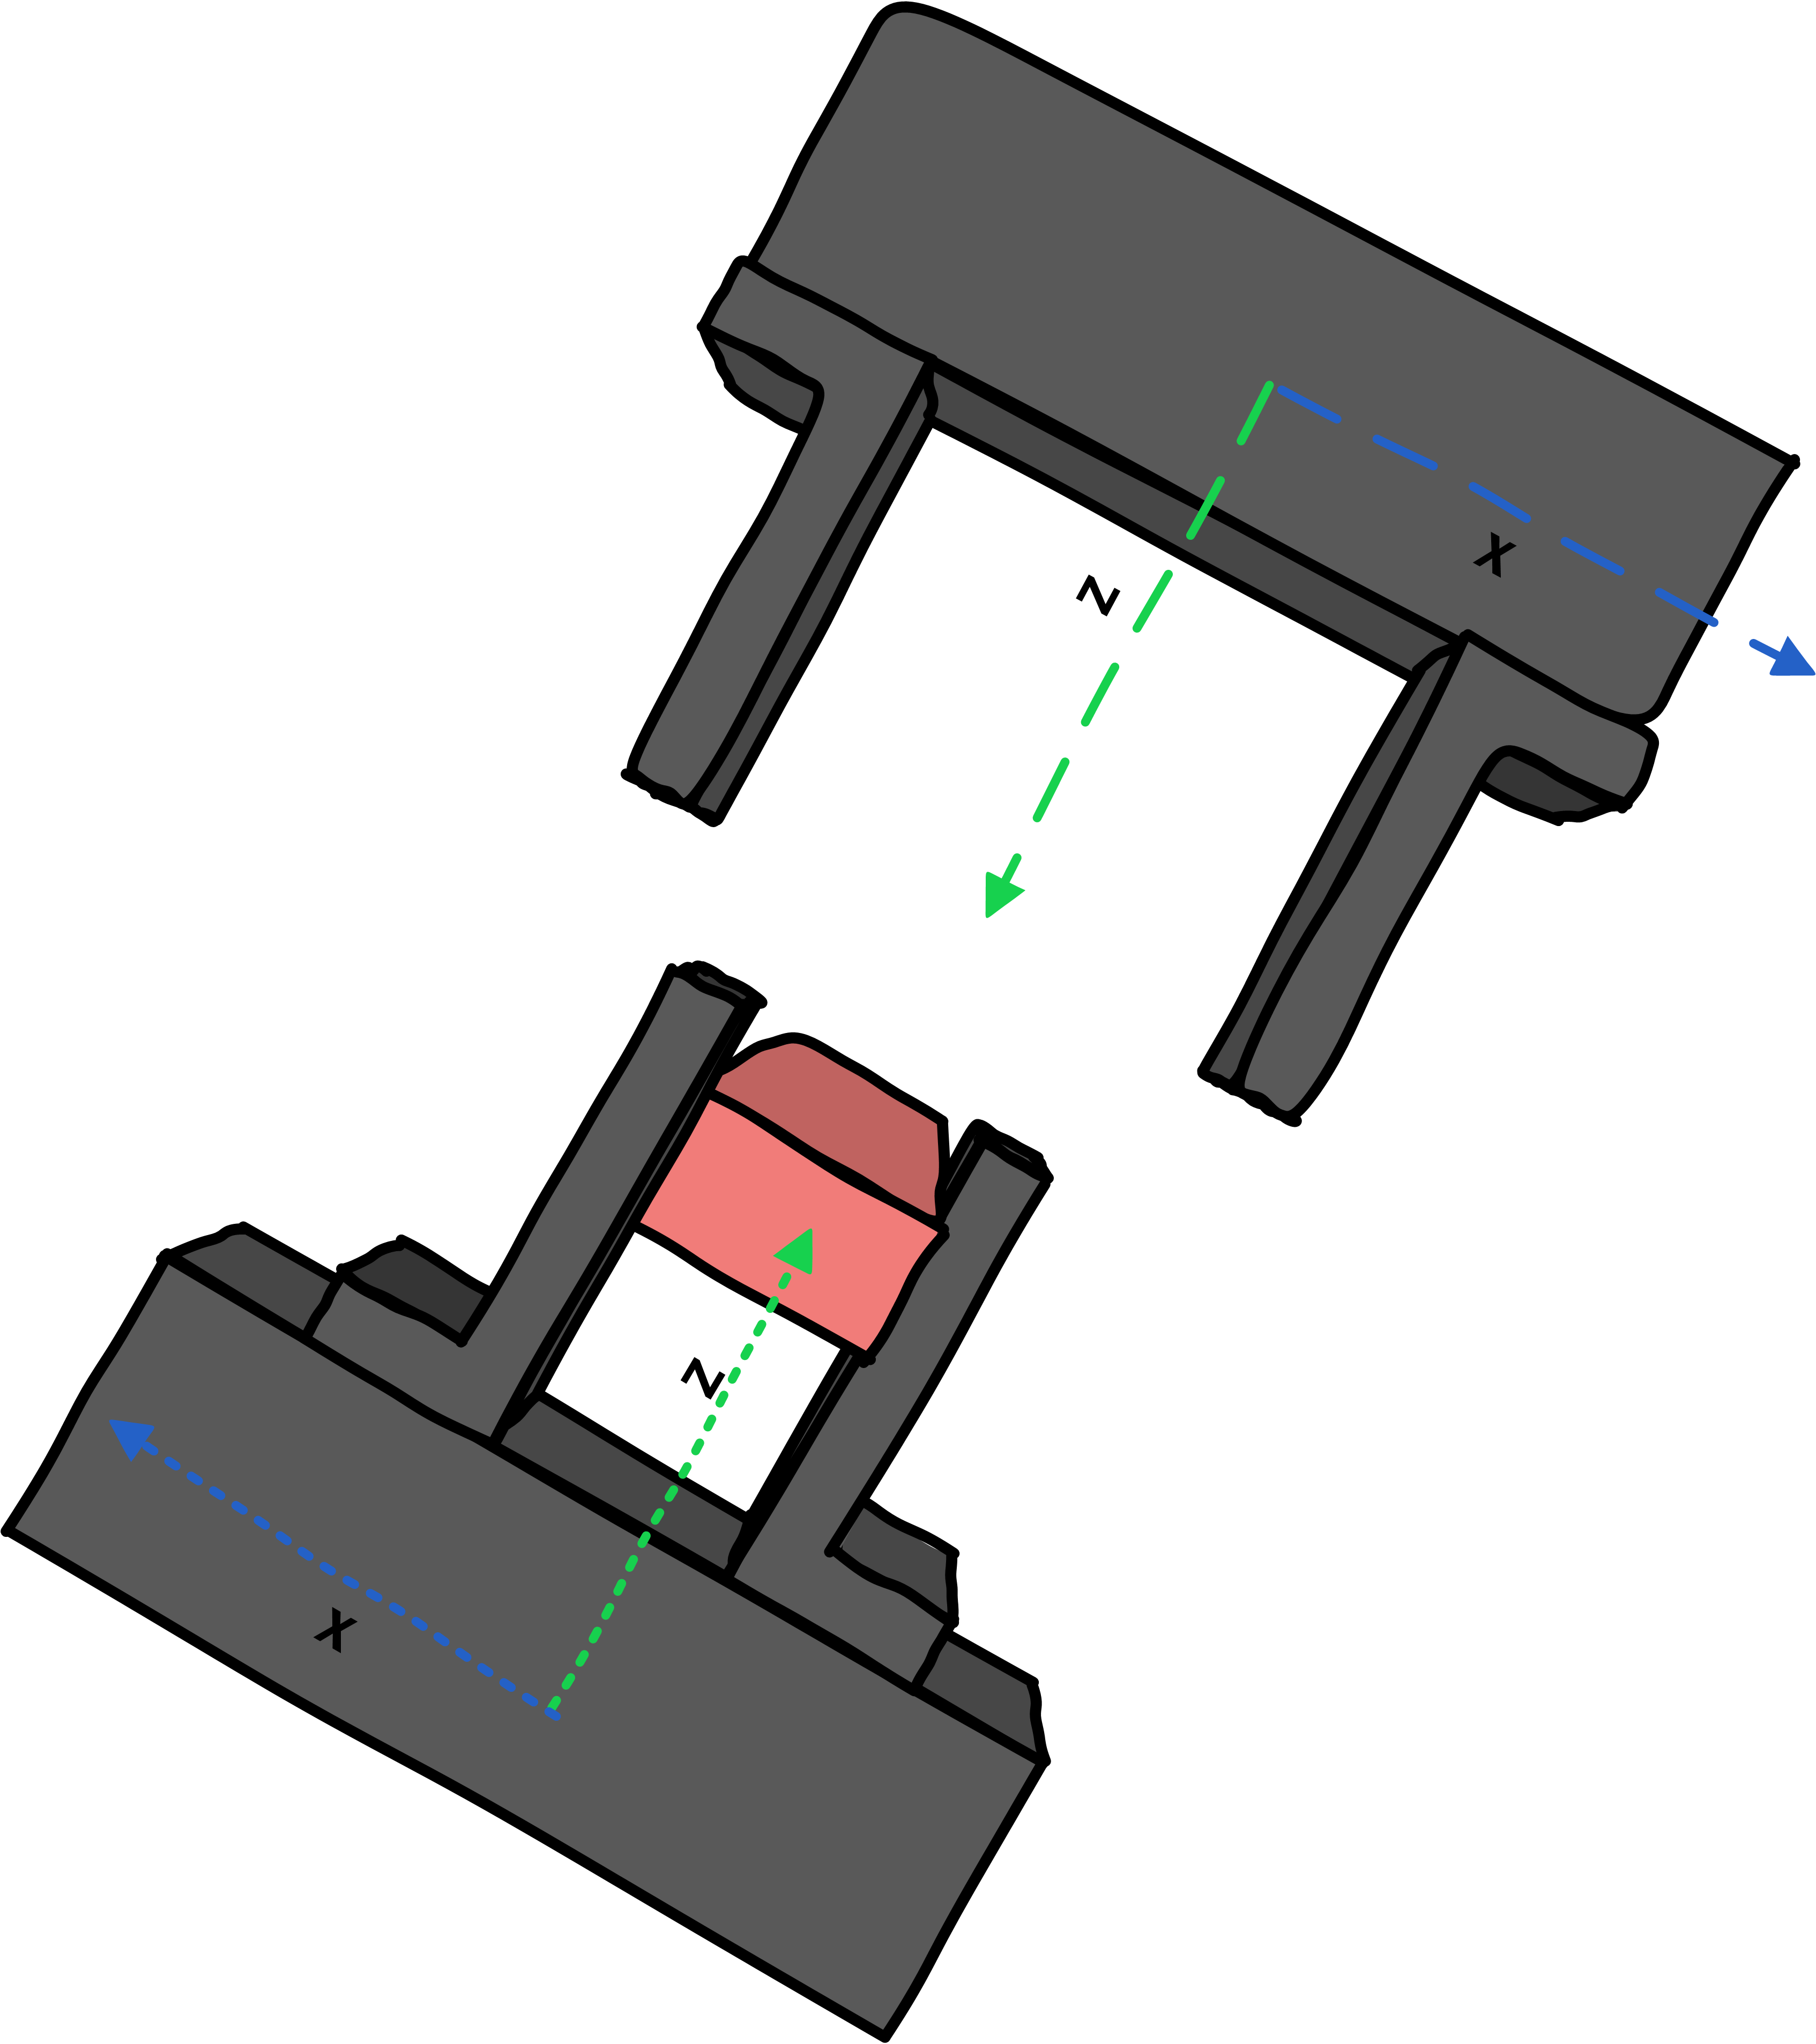
\includegraphics[scale=0.45]{fig/grip1}
 		\label{fig:grip1}}
 	\hfill
 	\subfigure[Translation($T_\tau$) an der X-Achse (blau) des Objektes (rose) zur Kollisionsvermeidung der Finger (grau). Die minimale Länge der Translation beträgt die Hälfter der aufsummierten Breite der Finger.]{%
 		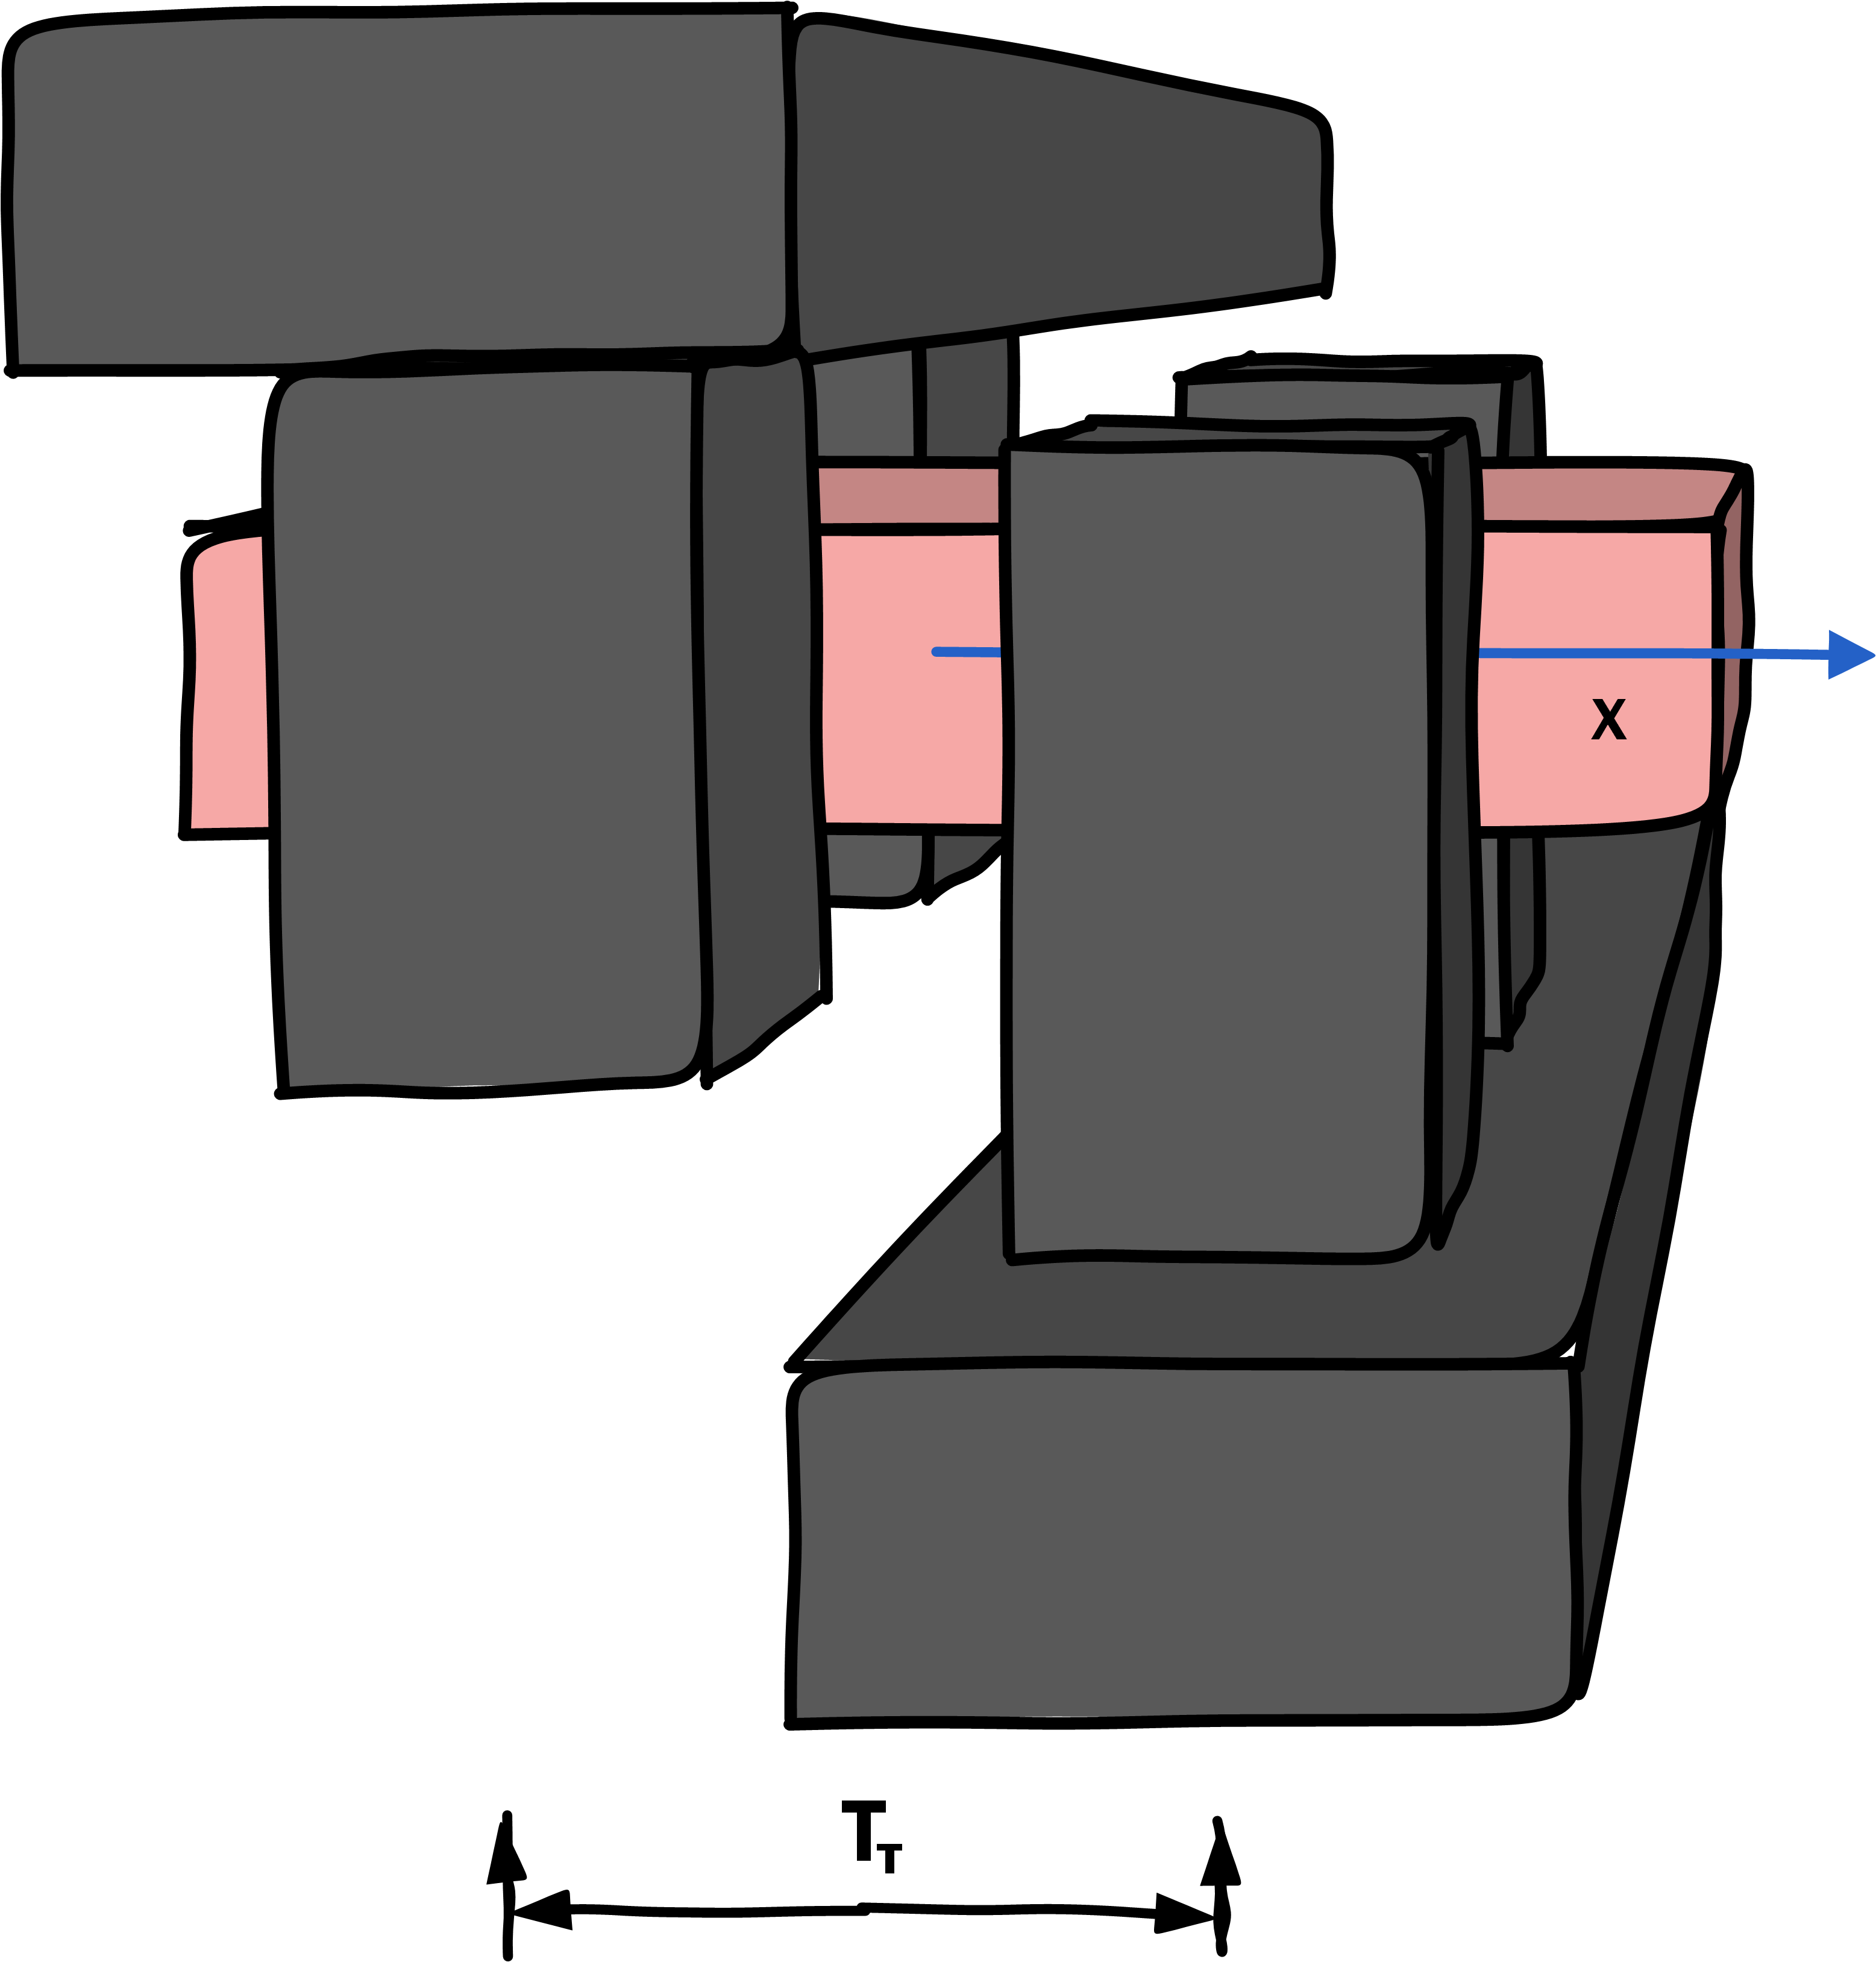
\includegraphics[scale=0.45]{fig/grip3}
 		\label{fig:grip3}}
 	
 	\caption{Greifer bei der Übergabe}
 	\label{fig:grip}
 \end{figure}

Da diese Funktionalität ein MR-Task ist, werden Nachrichten zwischen den Agenten ausgetauscht, um den Ablauf zu koordinieren. Dieser Nachrichtenaustausch wird in den folgenden Sequenz-Diagrammen dargestellt und analysiert. Dabei werden die drei Arten der Übergabe Geben (Abbildung \ref{fig:gripper1}), Nehmen (Abbildung \ref{fig:gripper2}) und Rendezvous (Abbildung \ref{fig:gripper3}) auf die Anzahl der Nachrichten $k$, sowie deren Komplexität, untersucht. Ein weiterer Aspekt ist das zeitliche Verhalten $t$ und der Unterschied im Ablauf der drei Varianten.

\begin{figure}
	\centering
	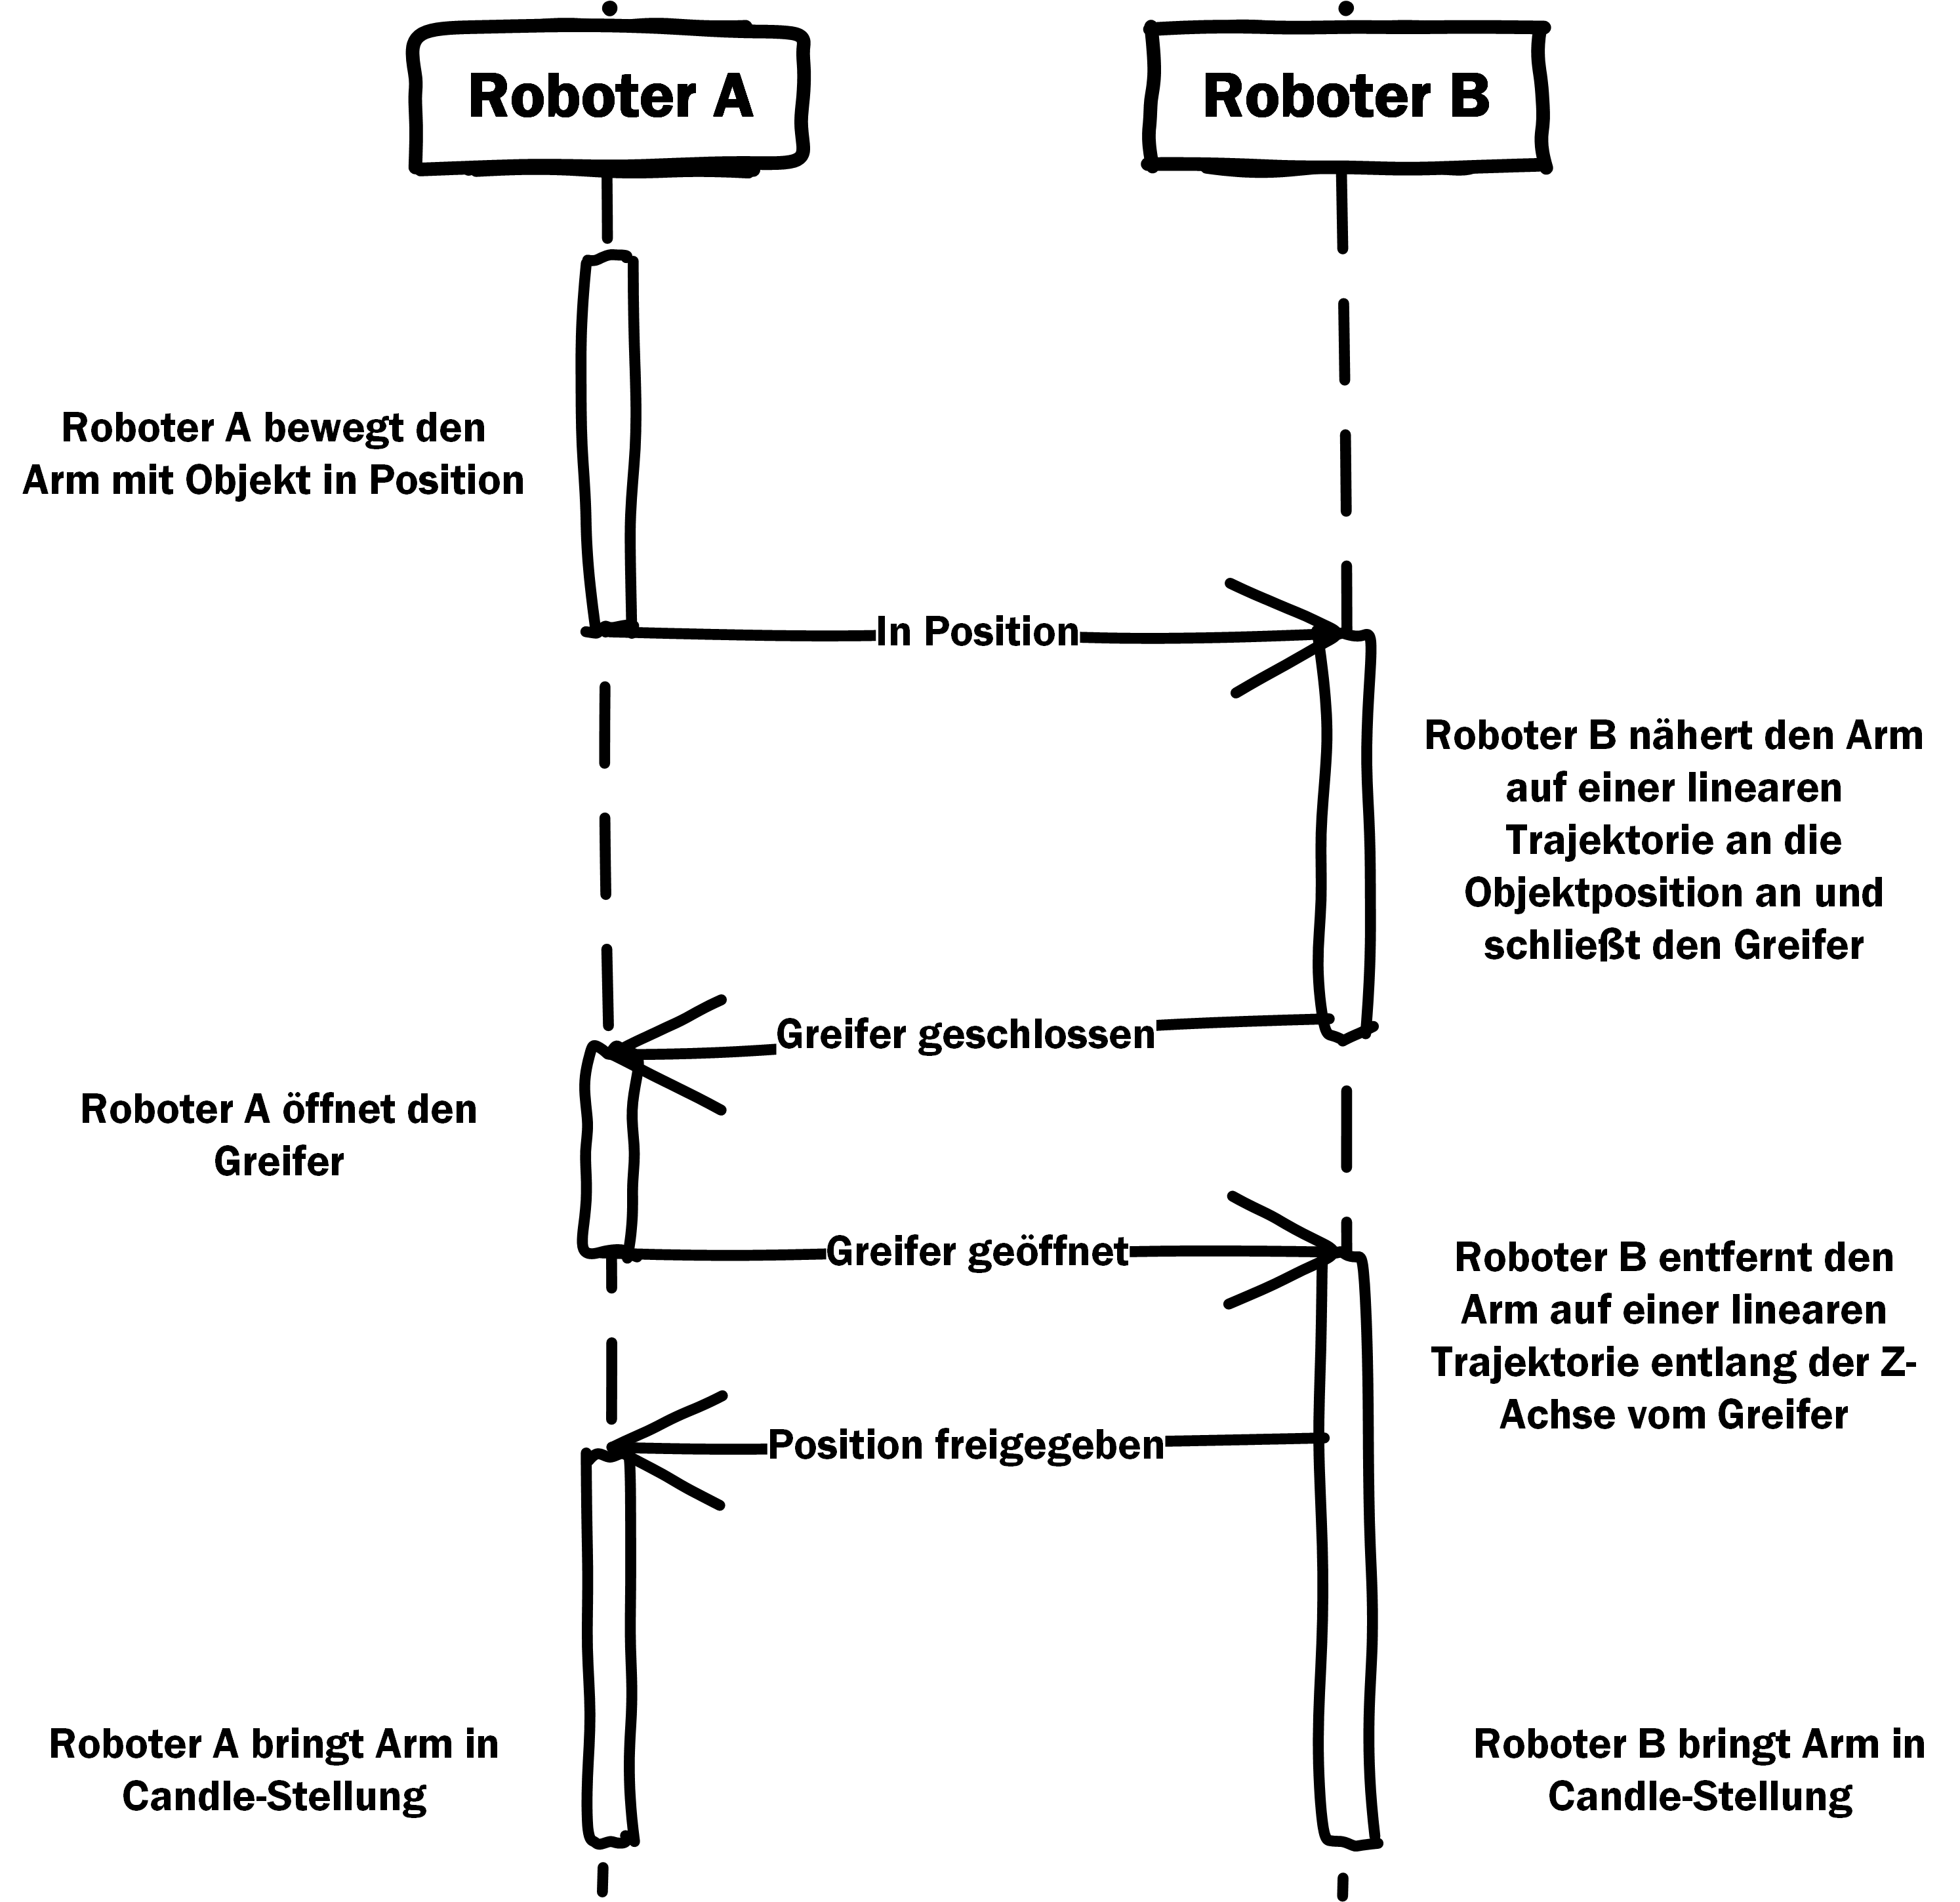
\includegraphics[scale=1.0]{fig/SeqGive}

	\caption[Sequenzdiagramm Geben]{Dieses Sequenzdiagramm zeigt den Ablauf des Gebens. Die Aktion wird dabei vom objekttragenden Roboter (A) initialisiert.}
		\label{fig:gripper1}
\end{figure}

Die in Abbildung \ref{fig:gripper1} dargestellte Variante des \textit{Gebens} wird von dem Roboter initialisiert, der das Objekt trägt (Roboter A). Nach Bestimmung der Übergabe Position und Orientierung bewegt sich zunächst Roboter A in die Pose. Dabei ist eine lineare Annäherung nicht nötig, da noch kein Kollisionspotential besteht. Anschließend wird eine einfache Bestätigung an Roboter B geschickt, der sich anschließend in Bewegung setzt. Diese besteht zunächst aus einer Positionierung nahe des Objektes. Der Greifer ist dabei schon geöffnet und dem anderen Greifer entgegengesetzt orientiert wie in Abbildung \ref{fig:grip1}. Folgend kommt die Annäherung auf der linearen Trajektorie entlang der Z-Achse an das Objekt. Sobald der Greifer in Position ist wird dieser geschlossen und eine einfache Bestätigung an den anderen Roboter gesendet. Dieser öffnet seinen Greifer und bestätigt ebenfalls. Durch diese Nachricht löst sich nun Roboter B, ebenfalls auf der Z-Achse, um das Objekt aus dem Greifer von Roboter A zu entfernen. Darauf folgt eine Freigabe an Roboter A, welcher sich nun auch von der Position entfernt, und der Übergang in die sichere Candle-Stellung.

Alle Nachrichten, die in dieser Variante ausgetauscht werden, sind einfache Bestätigungen oder Freigaben, die nur vom Zeitverhalten her dynamisch sind und keine weiteren Informationen beinhalten. Benötigt werden, ohne die Positionsbestimmung, vier Nachrichten zur vollständigen Koordinierung ($k_{Geben} = 4$). Für das Zeitverhalten gilt: $t_{Geben} = move_A + move_B + near_B + close_B + open_A + near_B + max(move_A, move_B)$ unter der Bedingung, dass $move_B \gg open_B$, da der Greifer von B während der Bewegung geöffnet wird. $move$ entspricht dabei der Zeit die für eine Bewegung von einer Pose in eine Zielpose benötigt wird, $near$ ist die Zeit für die positive oder negative Annäherung, $open$ und $close$ sind die benötigten Zeiten für das Öffnen und Schließen der Greifer.

\begin{figure}
		\centering
	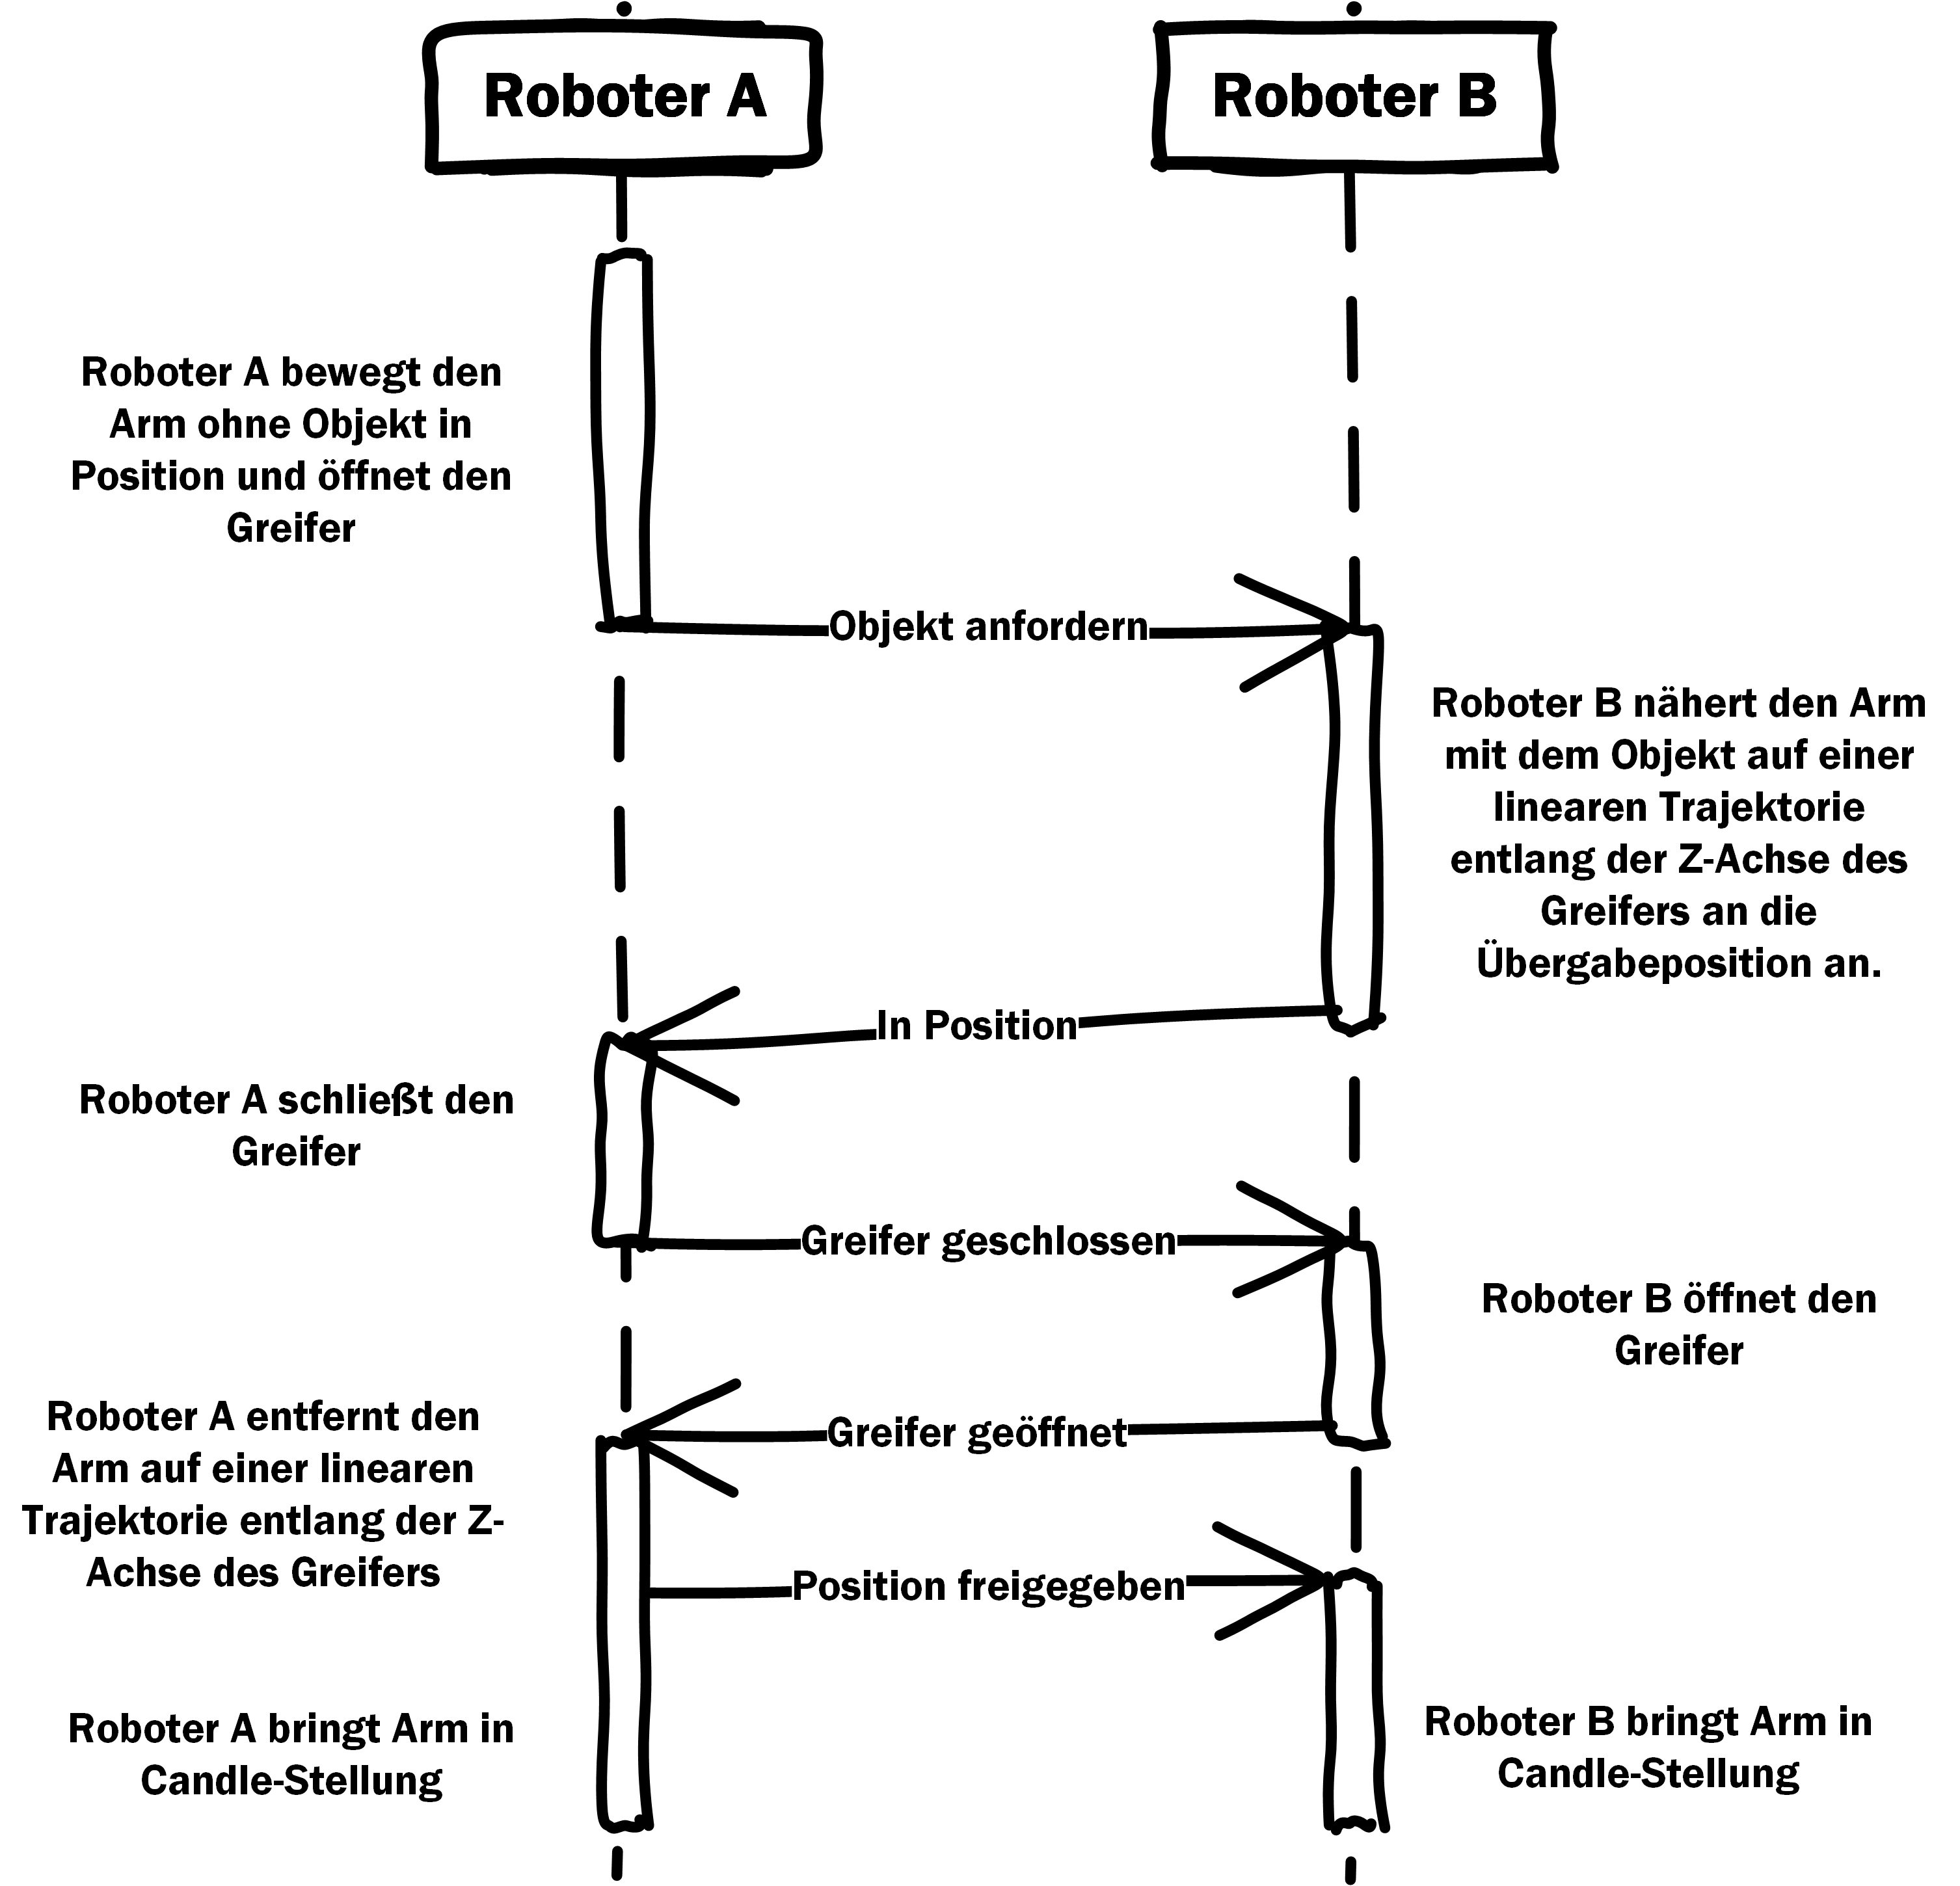
\includegraphics[scale=1.0]{fig/SeqTake}

\caption[Sequenzdiagramm Nehmen]{In diesem Sequenzdiagramm wird der Ablauf des Nehmens abgebildet. Die Aktion wird dabei vom objektlosen Roboter initialisiert.}
	\label{fig:gripper2}
\end{figure}

In Abbildung \ref{fig:gripper2} ist das \textit{Nehmen} dargestellt. Im Gegensatz zum \textit{Geben} wird die Aktion vom dem Roboter initialisiert, an den das Objekt übergeben wird. Nach der Positionsbestimmung bewegt Roboter A den Greifer ohne Objekt an die Übergabeposition und öffnet diesen während der Bewegung. Anschließend fordert er das Objekt an. Darauf nähert sich Roboter B mit dem Objekt auf der linearen Trajektorie entlang der Z-Achse dem Greifer A an und führt den Gegenstand zwischen den Fingern von Greifer A ein. Nach einer Positionsbestätigung schließt Roboter A den Greifer. In diesem Zustand wird das Objekt von beiden Robotern fixiert. Nach der Schließung des Greifers schickt Roboter A eine Nachricht an Roboter B, welcher nun seinen Greifer öffnet und dies mit einer Nachricht bestätigt. Roboter A entfernt nun das Objekt aus dem Greifer von Roboter B und gibt die Position frei nachdem er den Kollisionsraum verlassen hat. Anschließend bewegen beide Roboter die Arme in die sichere Candle-Stellung.

Der Nachrichtenaufwand dieser Variante beträgt $k_{Nehmen} = 5$. Wie beim \textit{Geben}, ist die Komplexität der Nachrichten eher gering, da es sich nur um zeitkritische Freigaben handelt. Für das Zeitverhalten gilt, unter den gleichen Bedingungen und Angaben wie beim \textit{Geben}: $t_{Nehmen} = move_A + move_B + near_B + close_A + open_B + near_A + max(move_A, move_B)$.


\begin{figure}
		\centering
	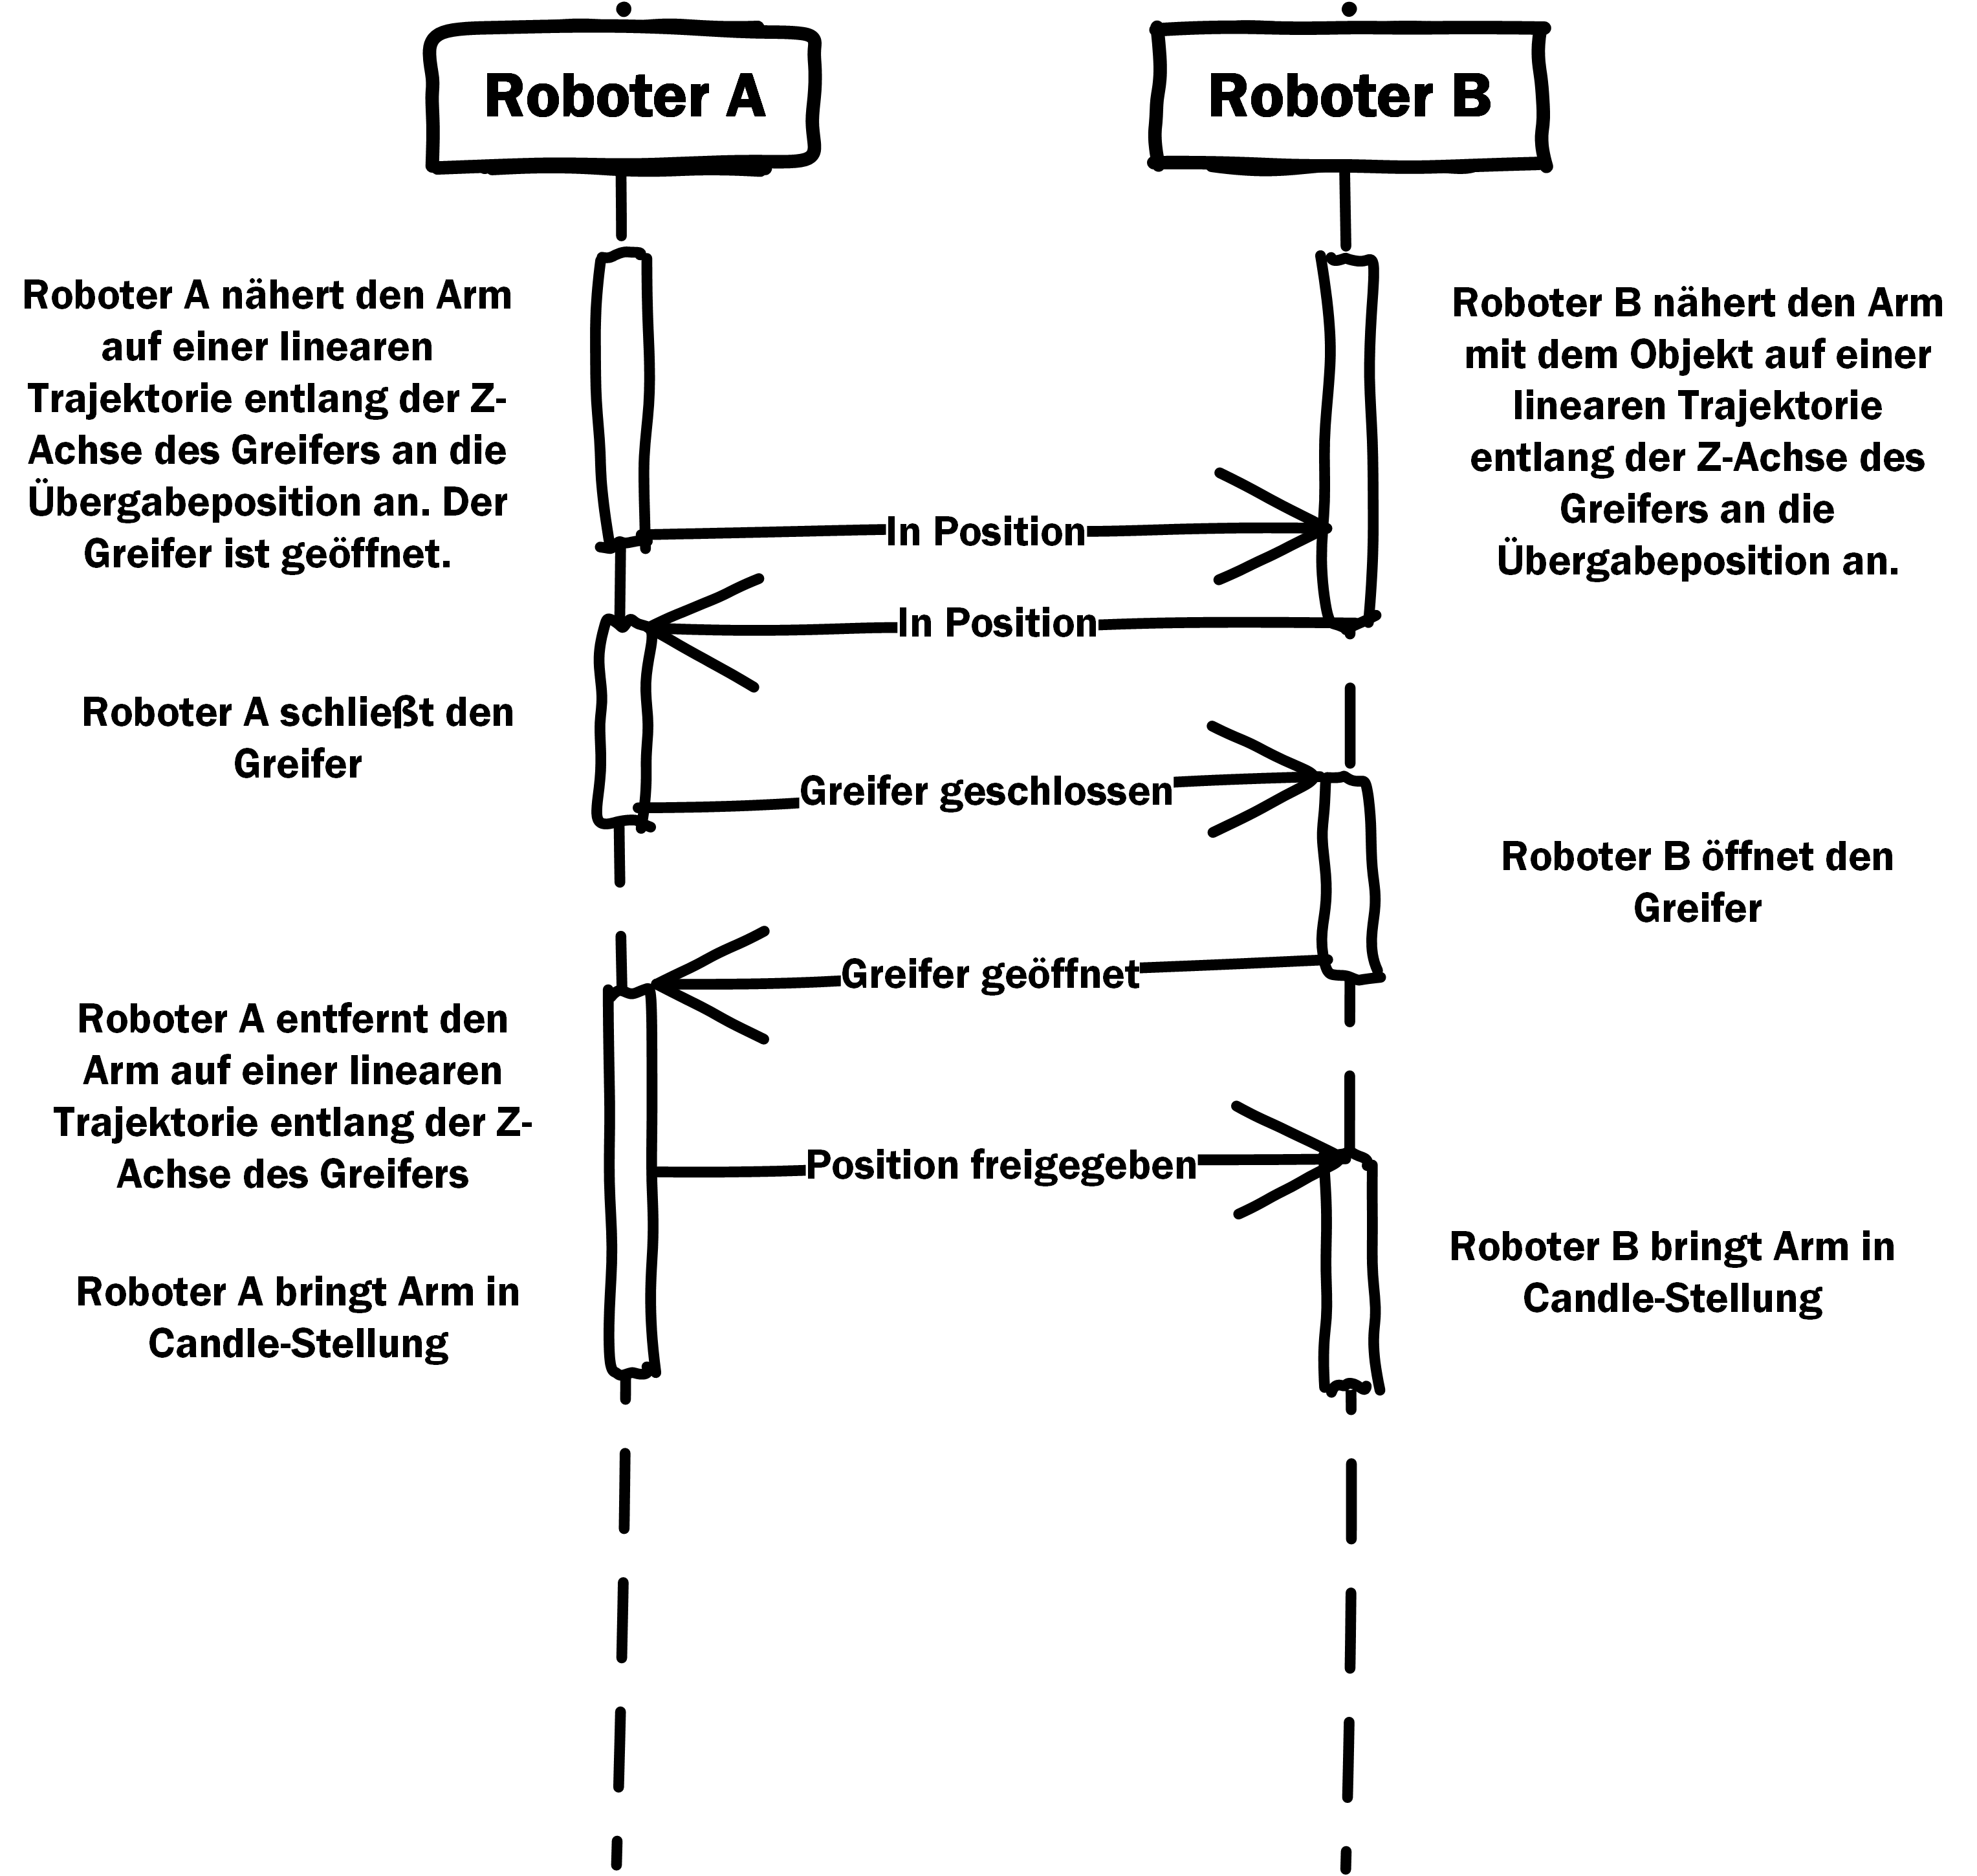
\includegraphics[scale=1.0]{fig/SeqRond}

\caption[Sequenzdiagramm Rendezvous]{Dieses Sequenzdiagramm zeigt die Rendezvous Variante der Übergabe. Die Aktion kann von beiden Agenten initialisiert.}
\label{fig:gripper3}
\end{figure}



Die Rendezvous-Übergabe in Abbildung \ref{fig:gripper3} wird die Initialisierungsbewegung nicht explizit von einem Roboter ausgeführt, sondern von beiden gleichzeitig. Dabei bewegen sich zunächst beide Arme auf die Übergabeposition, wobei sich beide Greifer das letzte Wegstück auf der linearen Trajektorie annähern. Beide Roboter bestätigen ihre Position, sobald sie diese erreicht haben. Anschließend schließt der Roboter A, ohne Objekt, den Greifer und bestätigt.Roboter B öffnet den Greifer und übergibt so das Objekt. Wie bei den anderen Varianten bewegt sich Roboter A nach einer Nachricht nun mit Objekt auf einer linearen Bahn von Greifer B weg. Nach der anschließenden Positionsfreigabe bewegen sich beide Roboter in die sichere Candle-Stellung.

Die Nachrichtenkomplexität ist bei dieser Variante etwas höher, als bei den anderen. Den Unterschied macht die erste Koordinierung, nachdem beide Arme in Position gegangen sind, da nicht definiert ist, welcher Roboter zuerst die Stellung erreicht und somit die Reihenfolge der Nachrichten nicht definiert ist. Die Komplexität des Inhaltes bleibt bei dieser Variante genauso gering, wie bei den anderen Variante, da es sich nur um Bestätigungen handelt. Die Anzahl der Nachrichten für diese Variante ist $k_{Rendezvous} = 5$. Für das Zeitverhalten gilt, unter den bekannten Bedingungen und Angaben:  $t_{Rendezvous} = max(move_A + near_A, move_B + near_B) + close_A + open_B + near_A + max(move_A, move_B)$.

Ein Vergleich der Kennzahlen der Varianten zeigt, dass der Koordinierungsaufwand beim \textit{Geben} am geringsten ist. Dies liegt vor allem an der Anzahl der Nachrichten: $k_{Geben} < k_{Nehmen} = k_{Rendezvous}$. Außerdem ist die Komplexität der Nachrichten untereinander identisch, mit der Ausnahme am Anfang der \textit{Rendezvous}-Variante. Für das Zeitverhalten gilt $t_{Rendezvous} < t_{Geben} = t_{Nehmen}$. Dies liegt vor allem an der Parallelisierung der Bewegung am Anfang der Aktion.


\paragraph{Einordnung}
Diese Funktion ist eng-gekoppelt und benötigt einen hohen Aufwand an Koordinierung. Neben der Übergabeposition und -orientierung müssen auch die Zeitvorgaben für das Öffnen und Schließen der Greifer, sowie die Bewegungen koordiniert werden. Dies macht diese Funktionalität zur komplexesten im ganzen System. Dies liegt vor allem daran, dass diese Funktion als MR-Task eingeordnet wird, da sie von zwei Agenten zusammen ausgeführt wird. Diese Agenten sollten Multi-Task fähig sein, da einige Subtasks parallel ausgeführt werden sollen, zum Beispiel das Öffnen des Greifers, während der Arm in eine Position fährt. Ebenfalls komplex ist die Positionsbestimmung der Übergabe. Zunächst müssen dabei die beiden Arbeitsräume einen Schnittraum aufweisen. Eine notwendige Positionskorrektur kann dabei nur vom mobilen Roboter ausgeführt werden. Dies muss unter anderem in der Konfiguration berücksichtigt werden. Dadurch steigt auch der Konfigurationsaufwand für die Aufgabe, da sichergestellt werden muss, dass die Arbeitsräume der beiden Roboter sich überhaupt schneiden können. Weitere Aspekte der Konfiguration sind die Kompatibilität der Greifer zum Objekt und die Erreichbarkeit der nachfolgenden Ziele.


\subsection{Agenten}
Aus den Nicht-Funktionalen Anforderungen und den Funktionen lassen sich die folgenden Agenten im MRS extrahieren. Diese Agenten bestehen aus den Sensoren aus Kapitel \ref{sec:aufbau-sensoren} und den Robotern Rose und Dummy. Für die Roboter steht die Zuweisung der Funktionen und Rollen im System fest, die anderen Aktoren und Sensoren werden den Funktionen zugewiesen. Für Funktionen bei denen unterschiedliche Sensoren oder Aktoren zur Verfügung stehen wird evaluiert welcher Hardware die Funktion am besten löst.

\subsubsection{Raumüberwachung}
Die Raumüberwachung ist zur Identifizierung und Lokalisierung von Objekten zuständig (siehe $f_2$\ref{sec:funraum}). Dabei soll das Kamerasystem eine große Fläche mit einer hohen Auflösung observieren. Als Hardware Lösungen standen dabei das XTion Kamera System oder der Argos3D Sensor zur Auswahl. Da der Tiefensensor jedoch eine kleinere Auflösung als die XTion hat und kein Farbbild liefert, wird für die Umsetzung des MRS die XTion ausgewählt. Diese wurde plangemäß nach Abbildung \ref{fig:basic-aufbau-teststand} und \ref{fig:basic-aufbau-teststandh} an der Wand montiert. Zur Befestigung wurde eine zusätzliche Halterung mit dem 3D-Drucker gedruckt. Diese ermöglicht einen größeren Winkel in der Ausrichtung. Der eingestellte Winkel beträgt -62 \textdegree um die globale X-Achse. Durch die Höhe und den eingestellten Winkel ergibt sich eine Observerationsfläche auf der globalen X-Y-Ebene von 5,075 $m^2$. In Abbildung \ref{fig:imghawk} sieht man eine aufgenommene Punktwolke der angebrachten Kamera. Auf dieser ist die Trapezform der Punktwolke sehr gut sichtbar. Diese ergibt sich aus der Position und Orientierung der Kamera. Bedingt dadurch weisen nähere Objekte eine größere Punktdichte auf als entfernte Objekte. Auf der Abbildung sind zwei Bereiche ohne Punkte markiert. Die blaue Markierung zeigt auf eine Verschattung durch den Roboterarm. Der grüne Bereich weist viele schlecht gematchte Punkte zwischen Farb- und IR-Bild auf. Dies liegt vor allem an den schlecht reflektierten IR-Punkten auf dem Heizkörpergitter.

\begin{figure}
	\centering
	\includegraphics[scale=1.0]{fig/imghawk}
	\caption[Raumüberwachung Aufnahme]{Aufnahme der XTion als Raumüberwachung. Blaue Markierung: Toter Winkel der IR Aufnahme. Grüne Markierung: Heizkörper mit diffusen IR-Reflektionen.}
	\label{fig:imghawk}
\end{figure}

\subsubsection{Nahfelderkennung}
Die Nahfelderkennung setzt die Funktionalität $f_3$ (siehe \ref{sec:funnah}) um. Dabei wird der Sensor auf dem mobilen Roboter befestigt, um ein Objekt auch im Nahfeld identifizieren und lokalisieren zu können. Die Lokalisierung soll dabei wesentlich genau sein, als bei der Raumüberwachung. Zur Auswahl standen dabei wieder die XTion und der Argos3D Sensor. Der Vorteil des Sensors ist die geringe minimale Reichweite. Diese funktioniert schon ab 100 mm, während die XTion einen mindest Abstand von 800 mm braucht. So ist eine Montage des Argos Sensors am Greifer direkt möglich, während die XTion mit Abstand montiert werden muss. Nachteil ist die zusätzliche Stromversorgung, die der Sensor benötigt, und der fehlende Farbkanal. Dennoch wurde der erste Prototyp mit dem Argos3D Sensor entwickelt, da er direkt am Greifer montiert werden kann. Ziel des Prototypen war es die Punktwolke eines Objektes von dem planaren Hintergrund zu separieren. Der Prototyp nutzt dafür den RANSAC-Algorithmus mit einem Flächenmodell. Jedoch ergab sich schnell, dass dieser Ansatz nicht mit dem Sensor funktioniert. Die Abbildung \ref{fig:argos} zeigt drei Aufnahmen einer Punktwolke die mit dem Sensor aufgenommen wurden. Die Aufnahmen entstanden von einem Objekt, dass auf einem Tisch liegt. In der Abbildung \ref{fig:argostop} ist die Draufsicht auf die Punktwolke dargestellt. Dabei stellen die unterschiedlichen Farben die Intensität der gemessenen IR-Werte. Das Objekt ist auf dieser Ansicht nur durch die Gradienten der Intensität an den Konturen zu erkennen. Die Abbildung \ref{fig:argoside} ist eine Seitenansicht der selben Punktwolke. Das Objekt ist an den fehlenden Punkten in der Mitte der Punktwolke erkennbar. Diese Punkte sind nicht sichtbar, da die Punktwolke konvex gewölbt ist. Punkte die näher an der Kamera sind verschwinden somit aus dieser Perspektive hinter der restlichen Punktwolke. Die konvexe Wölbung der Punktwolke ist das Problem der Separierung mit einem planaren Modell. Damit das planare Modell auf die Punktwolke angewandt werden kann muss die Fehlerschranke des Algorithmus sehr hoch gesetzt werden. Dadurch werden aber auch die Punkte des Objektes in die Fläche eingeschlossen. Eine Alternative zum planaren Modell wäre die Anwendung eines sphärischen Modells. Dabei muss die Sphäre aber geschlossen sein und nicht nur einen Teilabschnitt der Oberfläche sein.  Die Abbildung \ref{fig:argospowside} zeigt nochmal die Seitenansicht. Diesmal wurde jedoch der Sensor mit einer zusätzlichen externen Stromquelle versehen. Dieses ergab immer noch eine gekrümmte Oberfläche, welche jedoch schwächer ausgeprägt war als vorher. Ein Versuch die Krümmung aus der Punktwolke herauszurechnen, ähnlich wie bei einer Fischaugenlinse, endete in ziemlichen Abweichungen der Punkte, da die Entfernung zur Oberfläche und die Linsenkrümmung unbekannt ist.

\begin{figure}
	\centering
	\subfigure[Topansicht der Punktwolke, die Farben repräsentieren die Intensität der zurückgeworfenen IR-Strahlen. In der Mitte sind die Umrisse des Objektes erkennbar. Am Rand sind einige abweichende Punkte zu sehen.]{%
		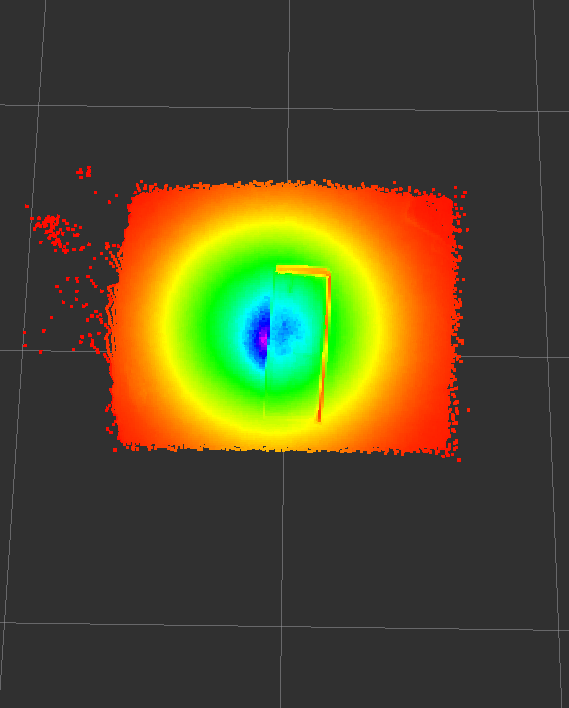
\includegraphics[scale=0.3]{fig/argostop}
		\label{fig:argostop}}
	\hfill
	\subfigure[Seitenansicht der Punktwolke. Sichtbar sind in der Mitte das Objekt und die kubische Grundform der Punktwolke, die eigentlich der planaren Ebene entsprechen sollte.]{%
		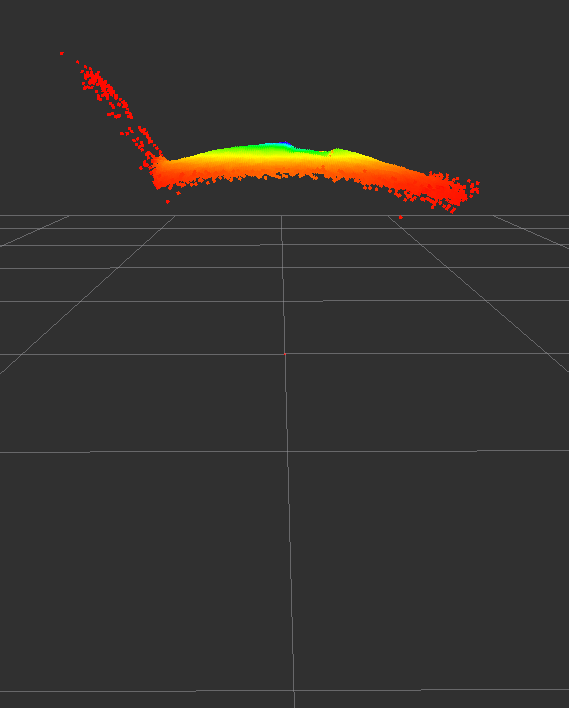
\includegraphics[scale=0.3]{fig/argoside}
		\label{fig:argoside}}
	\hfill
	\subfigure[Seitenansicht der Punktwolke mit zusätzlicher Stromversorgung am Sensor. Sichtbar ist wieder das Objekt in der Mitte. Die Krümmung der Oberfläche ist schwächer als bei Abbildung \ref{fig:argoside}]{%
		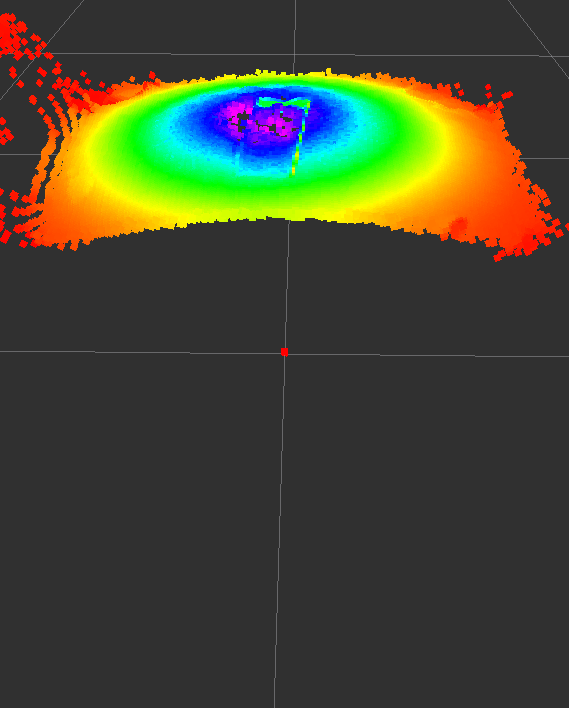
\includegraphics[scale=0.3]{fig/argospowside}
		\label{fig:argospowside}}
	\caption[Argos3D Punktwolke]{Aufgenommene Punktwolke mit dem Argos3D Sensor. Abgebildet ist ein quaderförmiges Objekt auf einem Tisch.}
	\label{fig:argos}
\end{figure}

Nach den negativen Tests mit dem Sensor folgten Überlegungen, ob man die XTion Kamera für die Naherkennung einsetzen kann. Problem war die große minimal Distanz für die Erkennung. Damit die benötigten 800 mm zum Boden erreicht werden, ist die Kamera am Greifer montiert, siehe Abbildung \ref{fig:xtionarm} Befindet sich der Arm in der Candle-Pose ist die Kamera 800 mm vom Untergrund entfernt und erfasst das Feld direkt vor der mobilen Plattform. TODO Infos. Durch eine Drehung des Armes, um das erste oder fünfte Gelenk, kann das Sichtfeld der Kamera erweitert werden. Jedoch gab es auch bei den ersten Tests mit der Kamera einige Probleme. Durch den eingebauten Weißabgleich wurde die Helligkeit des Bildes bei einer zu starken Einstrahlung reduziert. Das führte im Labor unter anderem zu einem schwarzen Bild und resultierte aus der Lichtreflexion der Aluminiumplatte die auf der mobilen Plattform montiert ist. Der Fehler konnte durch Abkleben der reflektierenden Oberfläche beseitigt werden.

\begin{figure}
	\centering
	\subfigure[Die XTion Kamera(rot) am Greifer montiert. Das Sichtfeld liegt vor der mobilen Plattform. Durch eine Drehung des Armes kann das Sichtfeld um den Roboter erweitert werden.]{%
		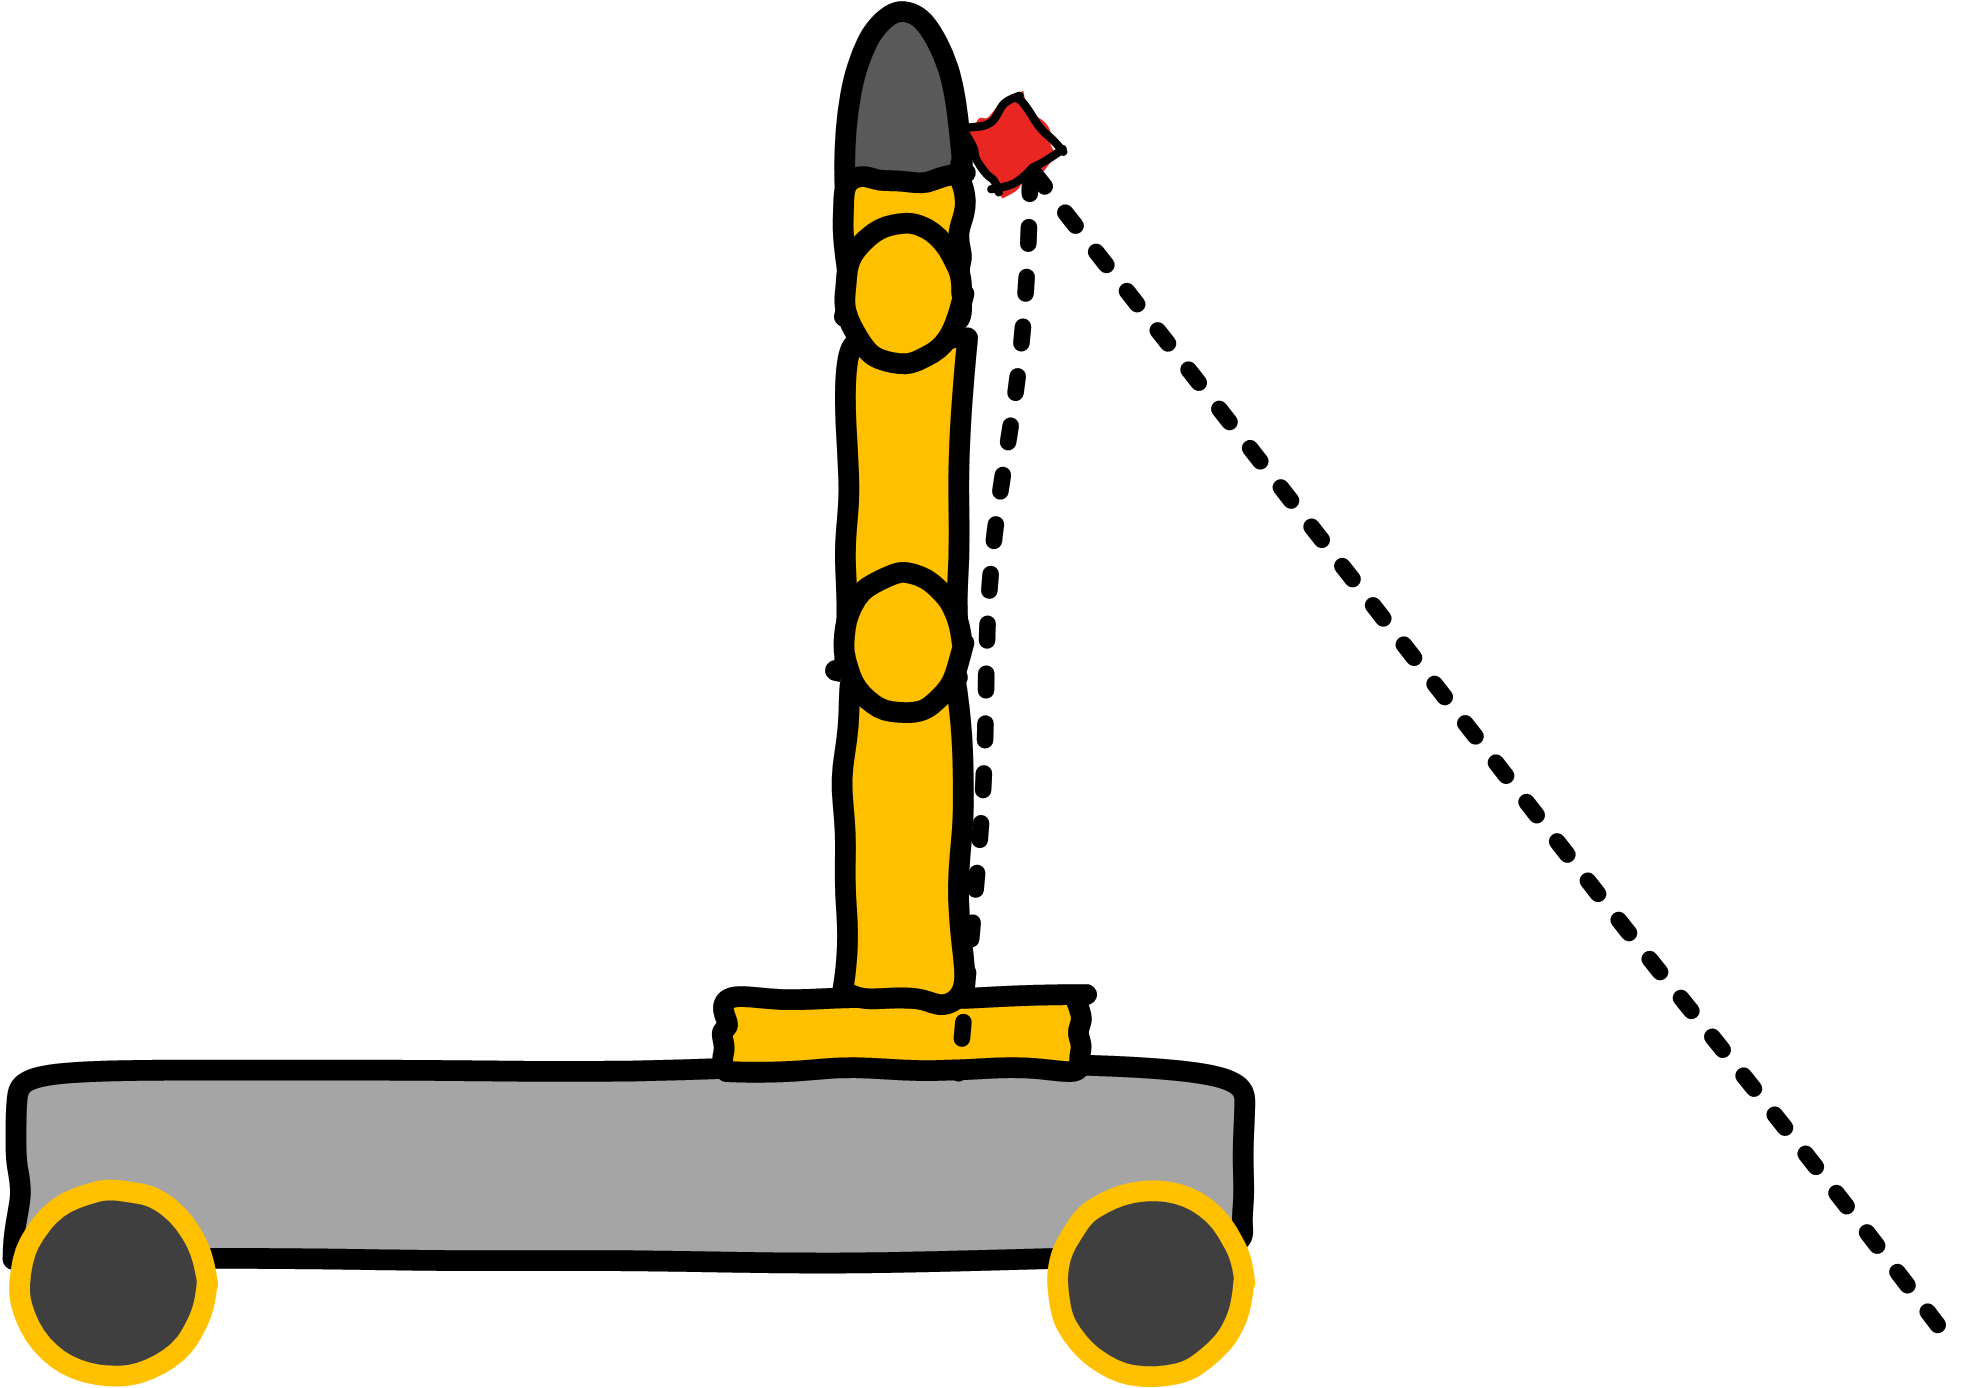
\includegraphics[scale=0.8]{fig/xtionarm}
		\label{fig:xtionarm}}
	\hfill
	\subfigure[TODO]{%
		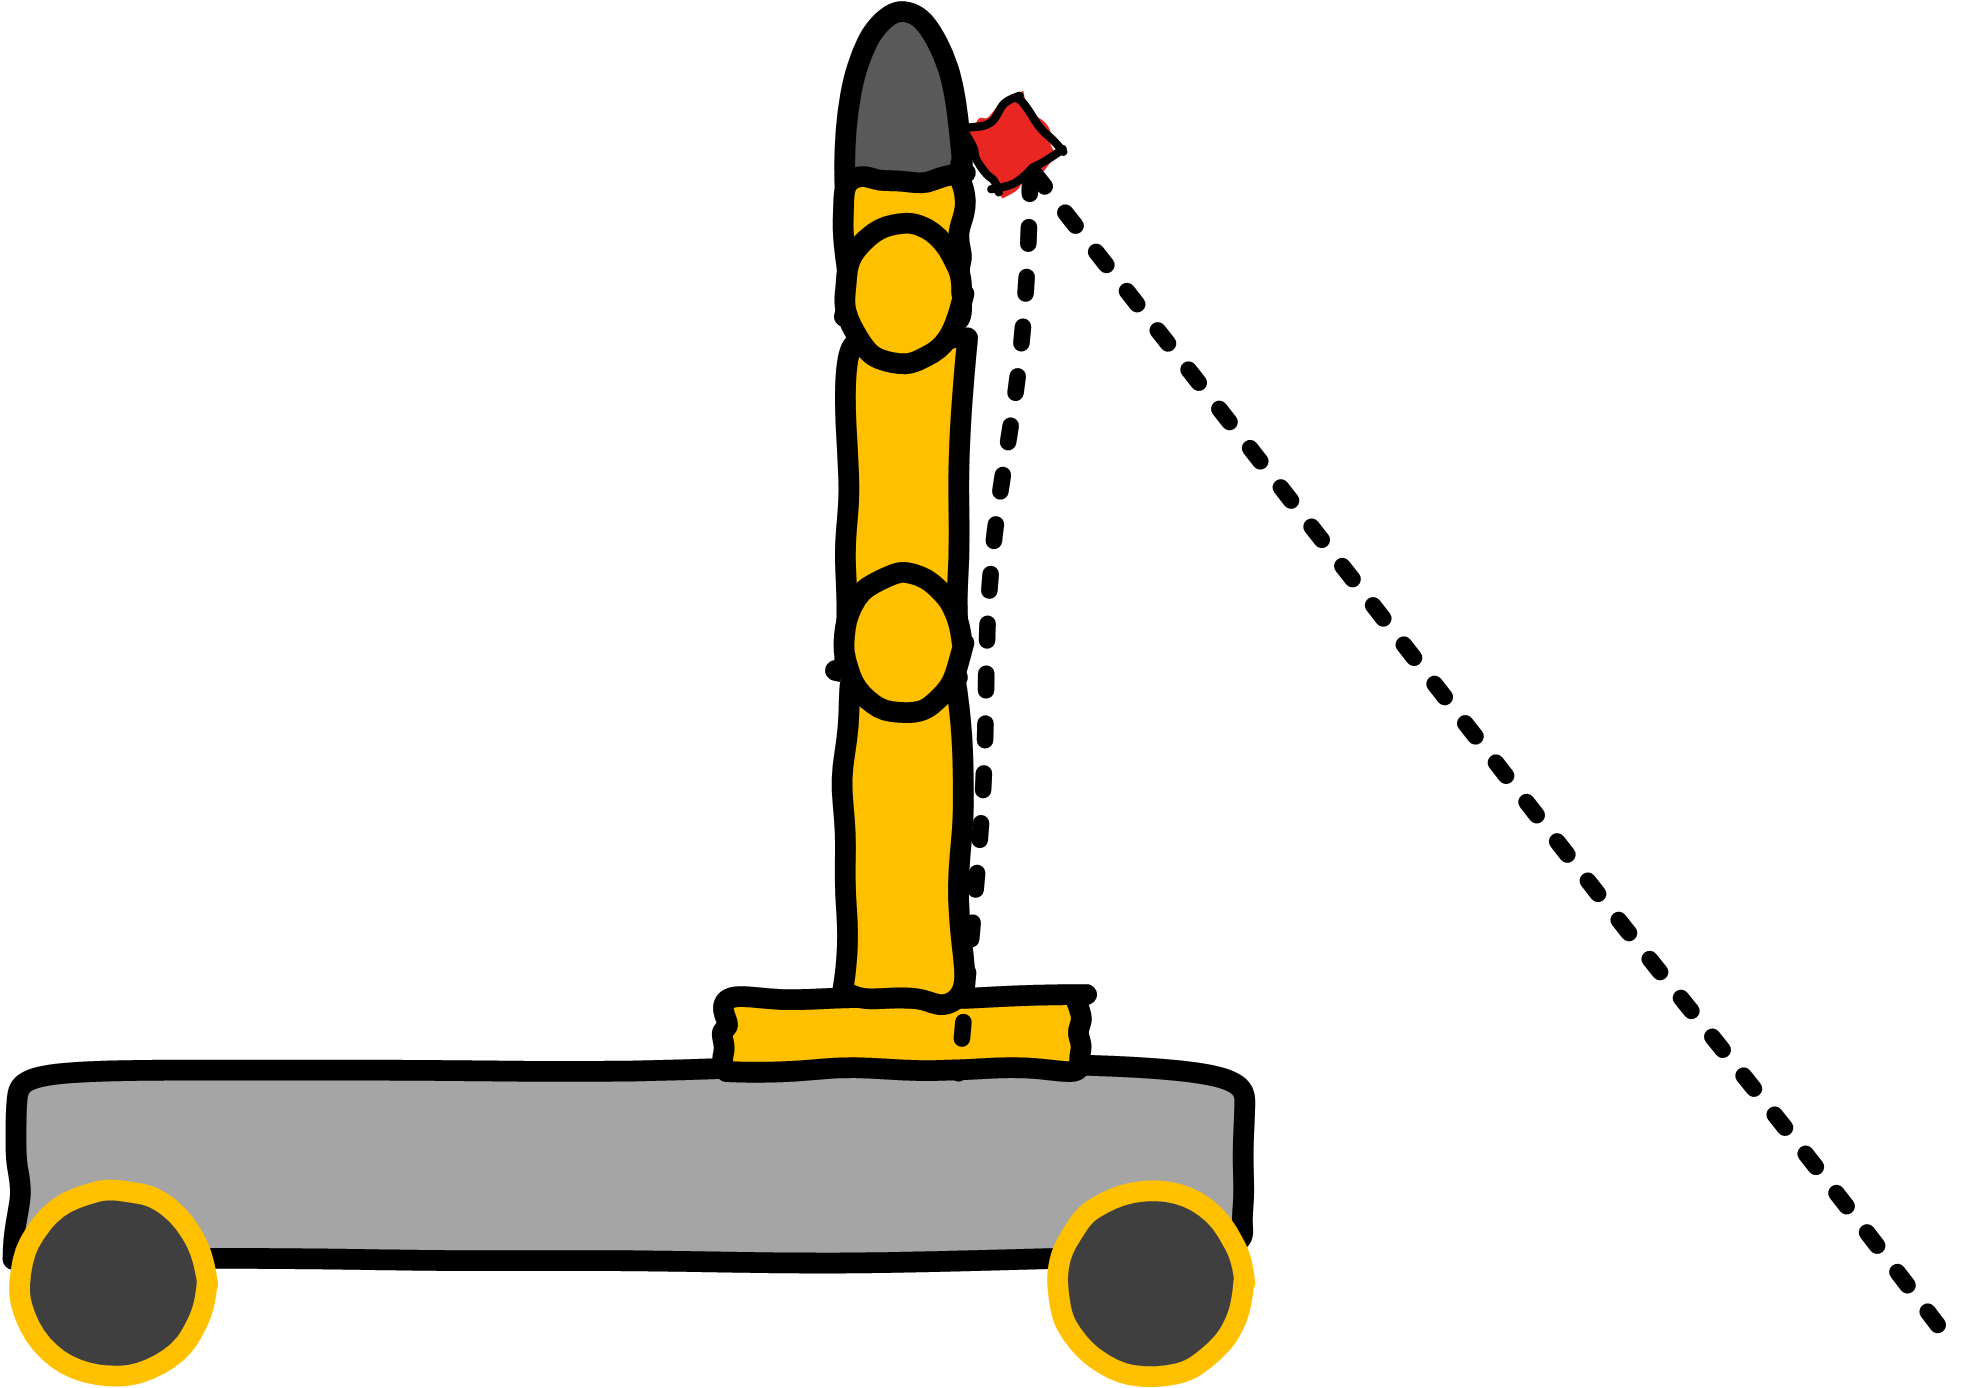
\includegraphics[scale=0.3]{fig/xtionarm}
		\label{fig:xtionarmbild}}
	\caption[XTion als Naherkennung]{Die Asus XTion als Hardware Lösung für die Naherkennung}
	\label{fig:xtionnah}
\end{figure}


\subsubsection{Lokalisierung}
Für die Lokalisierung, $f_4$ in Kapitel \ref{sec:funl}, sind alle Sensoren potenziell möglich. Die einfachste Variante wäre die Auswertung der Odometriedaten. Dazu wird die Geschwindigkeit der Plattform mit der Laufzeit multipliziert um den zurückgelegten Weg zu berechnen. Um die Genauigkeit zu bestimmen wurden im Rahmen dieser Arbeit Versuche durchgeführt. Dazu wurden zunächst linearen Bewegungen entlang einer Achse ausgeführt und gemessen. Anschließend wurden kombinierte lineare Bewegungen entlang der X- und Y-Achse getestet. Die dabei verwendeten Geschwindigkeiten und Laufzeiten wurden variiert. Gemessen wurde anschließend die zurückgelegte Distanz bei zehn Versuchen pro Messgruppe. Für die anschließende Auswertungen wurden die arithmetischen Mittelwerte für die absolute und relative Abweichung über den Versuchsgruppen berechnet. Die anschließende Bewertung wurde für die einzelnen Versuchsgruppen im Bezug aufeinander und der Geschwindigkeit, sowie Laufzeit vorgenommen. Dabei ergab sich, dass es eine starke positive Kovarianz zwischen Geschwindigkeit und Abweichung gibt. Diese liegt vor allem an den nicht sehr genauen Motoren-Controllern und dem Anhalten, da die Plattform nicht langsam negativ beschleunigt, sondern die Geschwindigkeit direkt auf null setzt. Auch die Kovarianz zwischen Laufzeit und Abweichung ist positiv ausgeprägt, erreicht aber nicht den Wert der Geschwindigkeit. Die größten relativen Abweichungen zeigen die kombinierten Bewegungen bei hohen Geschwindigkeiten. Auch die seitlichen Bewegungen auf der Y-Achse der Plattform zeigen starke Abweichungen. Diese sind auf die omnidirektionalen Räder zurückzuführen. Auffällig sind auch die hohen relativen Abweichungen bei kurzen Laufzeiten. Nach Beobachtung der mobilen Plattform lässt sich dies mit dem Schlupf der Räder und dem glatten staubigen Untergrund erklären. So scheinen die Räder zunächst durchzudrehen. Ein weiteres Problem scheint die Ansteuerung zu sein. Das Testprogramm zur Versuchssteuerung schickt zunächst asynchron das Signal mit den Geschwindigkeiten an die Motorensteuerung. Anschließend pausiert die Steuerung für die eingestellte Laufzeit, bevor das Stopp-Signal asynchron an die Motoren geschickt wird. Dabei entsteht eine unbekannte Verzögerung durch das asynchrone Steuersignal. Zusammengefasst ist diese Methodik alleine zur Lokalisierung des Roboters ungeeignet, da die Abweichungen zu groß sind. Eine mögliche Fehlerkorrektur ist auf Grund des hohen Standardfehlers und den zufälligen Umweltfaktoren (Schlupf und Signalverzögerung) nur schwer realisierbar.

Eine weitere Option zur Lokalisierung ist die visuelle Odometrie. Dabei wird der optische Fluss einer Bildsequenz genutzt um die eigene Geschwindigkeit und Positionsveränderung zu bestimmen. Dazu müssen zunächst in zeitlich aufeinanderfolgenden Bildern Features detektiert und untereinander zugewiesen werden. Durch die Veränderung der Position auf dem Bild aller Features entsteht ein Vektorfeld. Dieses wird zur Bewegungsschätzung der Kamera genutzt. Diese Methodik benötigt jedoch ein Kamerasystem mit einer geringen Verzögerungszeit. Das XTion Kamerasystem hat an dem Rechner von Dummy eine Verzögerung von einer Sekunde. An dem eingebauten Rechner in der mobilen Plattform beträgt die Verzögerung über drei Sekunden und die Bildrate unter ein Bild pro Sekunde, was für eine zuverlässige Ortung nicht reicht.

Auf der Entwicklungsseite des YouBots wird der Lasersensor Hokuyo URG-04LX-UG01 für die Navigation angeboten. Auch Peter Corke nutzt in \cite[Kapitel 6]{Corke2011} einen Hokuyo Lasersensor zur Navigation. Dabei stellt TODO SLAM er ein Kartenverfahren vor und nutzt den TODO. Ein Problem beim Mapping ist der gekidnappte Roboter. Diesem fehlen Informationen zu vorhergegangenen Position. Dies kann auf fehlerhaften Berechnungen oder fehlenden Sensordaten beruhen. Da vom Labor keine Karte existiert und das Erstellen dieser den zeitlichen Aufwand der Arbeit überschreitet, wird in dieser Arbeit mit einem Hybridverfahren zwischen Karten- und Odometriebasierter Lokalisierung gearbeitet. Dazu wird eine grobe Position mit Hilfe der Odometrie errechnet. Diese wird in regelmäßigen Abstände mit den Daten des Lasersensors korrigiert, um einen möglichen Schleppfehler zu verhindern.

\subsection{Architektur RATS}
In diesem Kapitel wird die Software-Architektur \textit{RATS} vorgestellt. RATS steht für \textit{Roboter Action and Task System} und setzt die Anforderungen für dieses MRS um. Dabei liegt ein besonderes Augenmerk auf der einfachen Erweiterbarkeit und Konfiguration des ganzen Systems. So können neue Aktoren und Sensoren ohne großen Aufwand und Veränderung des bestehenden Systems eingefügt werden. Im Folgenden werden das Konzept und die einzelnen Bestandteile der Architektur erklärt. Da das System auf ROS aufbaut wurde schon in der Architektur dem Package und Node Konzept gefolgt.

\subsubsection{Konzept}
Das Klassendiagramm in Abbildung \ref{fig:classrats} bildet die Architektur von RATS ab. Das Motiv hinter der Architektur ist die Zerlegung der Aufgaben in Actions und Tasks für Agenten in MRS. Jede Action entspricht dabei einer Funktion die ein Agent anbieten kann. Jede Task ist eine Abfolge von Actions, welche parallel oder seriell vom Agenten ausgeführt werden, und ist ebenfalls eine Action. Dadurch können Tasks eigene Subtasks ausführen. Jede Action und Task besitzt eine ID, durch diese ID kann einem Agenten mitgeteilt werden, welche Action oder Task er ausführen soll. Dieser Befehl kann von dem zentralen RATSCore oder jedem anderen Agenten im System ausgerufen werden. Die Agenten werden in dieser Architektur durch die RATSMember abgebildet. Jeder RATSMember besitzt eine Menge an Actions und Tasks, die von dem Agenten ausgeführt werden. Diese Menge an Actions und Tasks werden bei der Initialisierung an den RATSCore übertragen. Dieser übernimmt die Koordinierung und Konfigurierung im System.

\begin{figure}
	\centering
	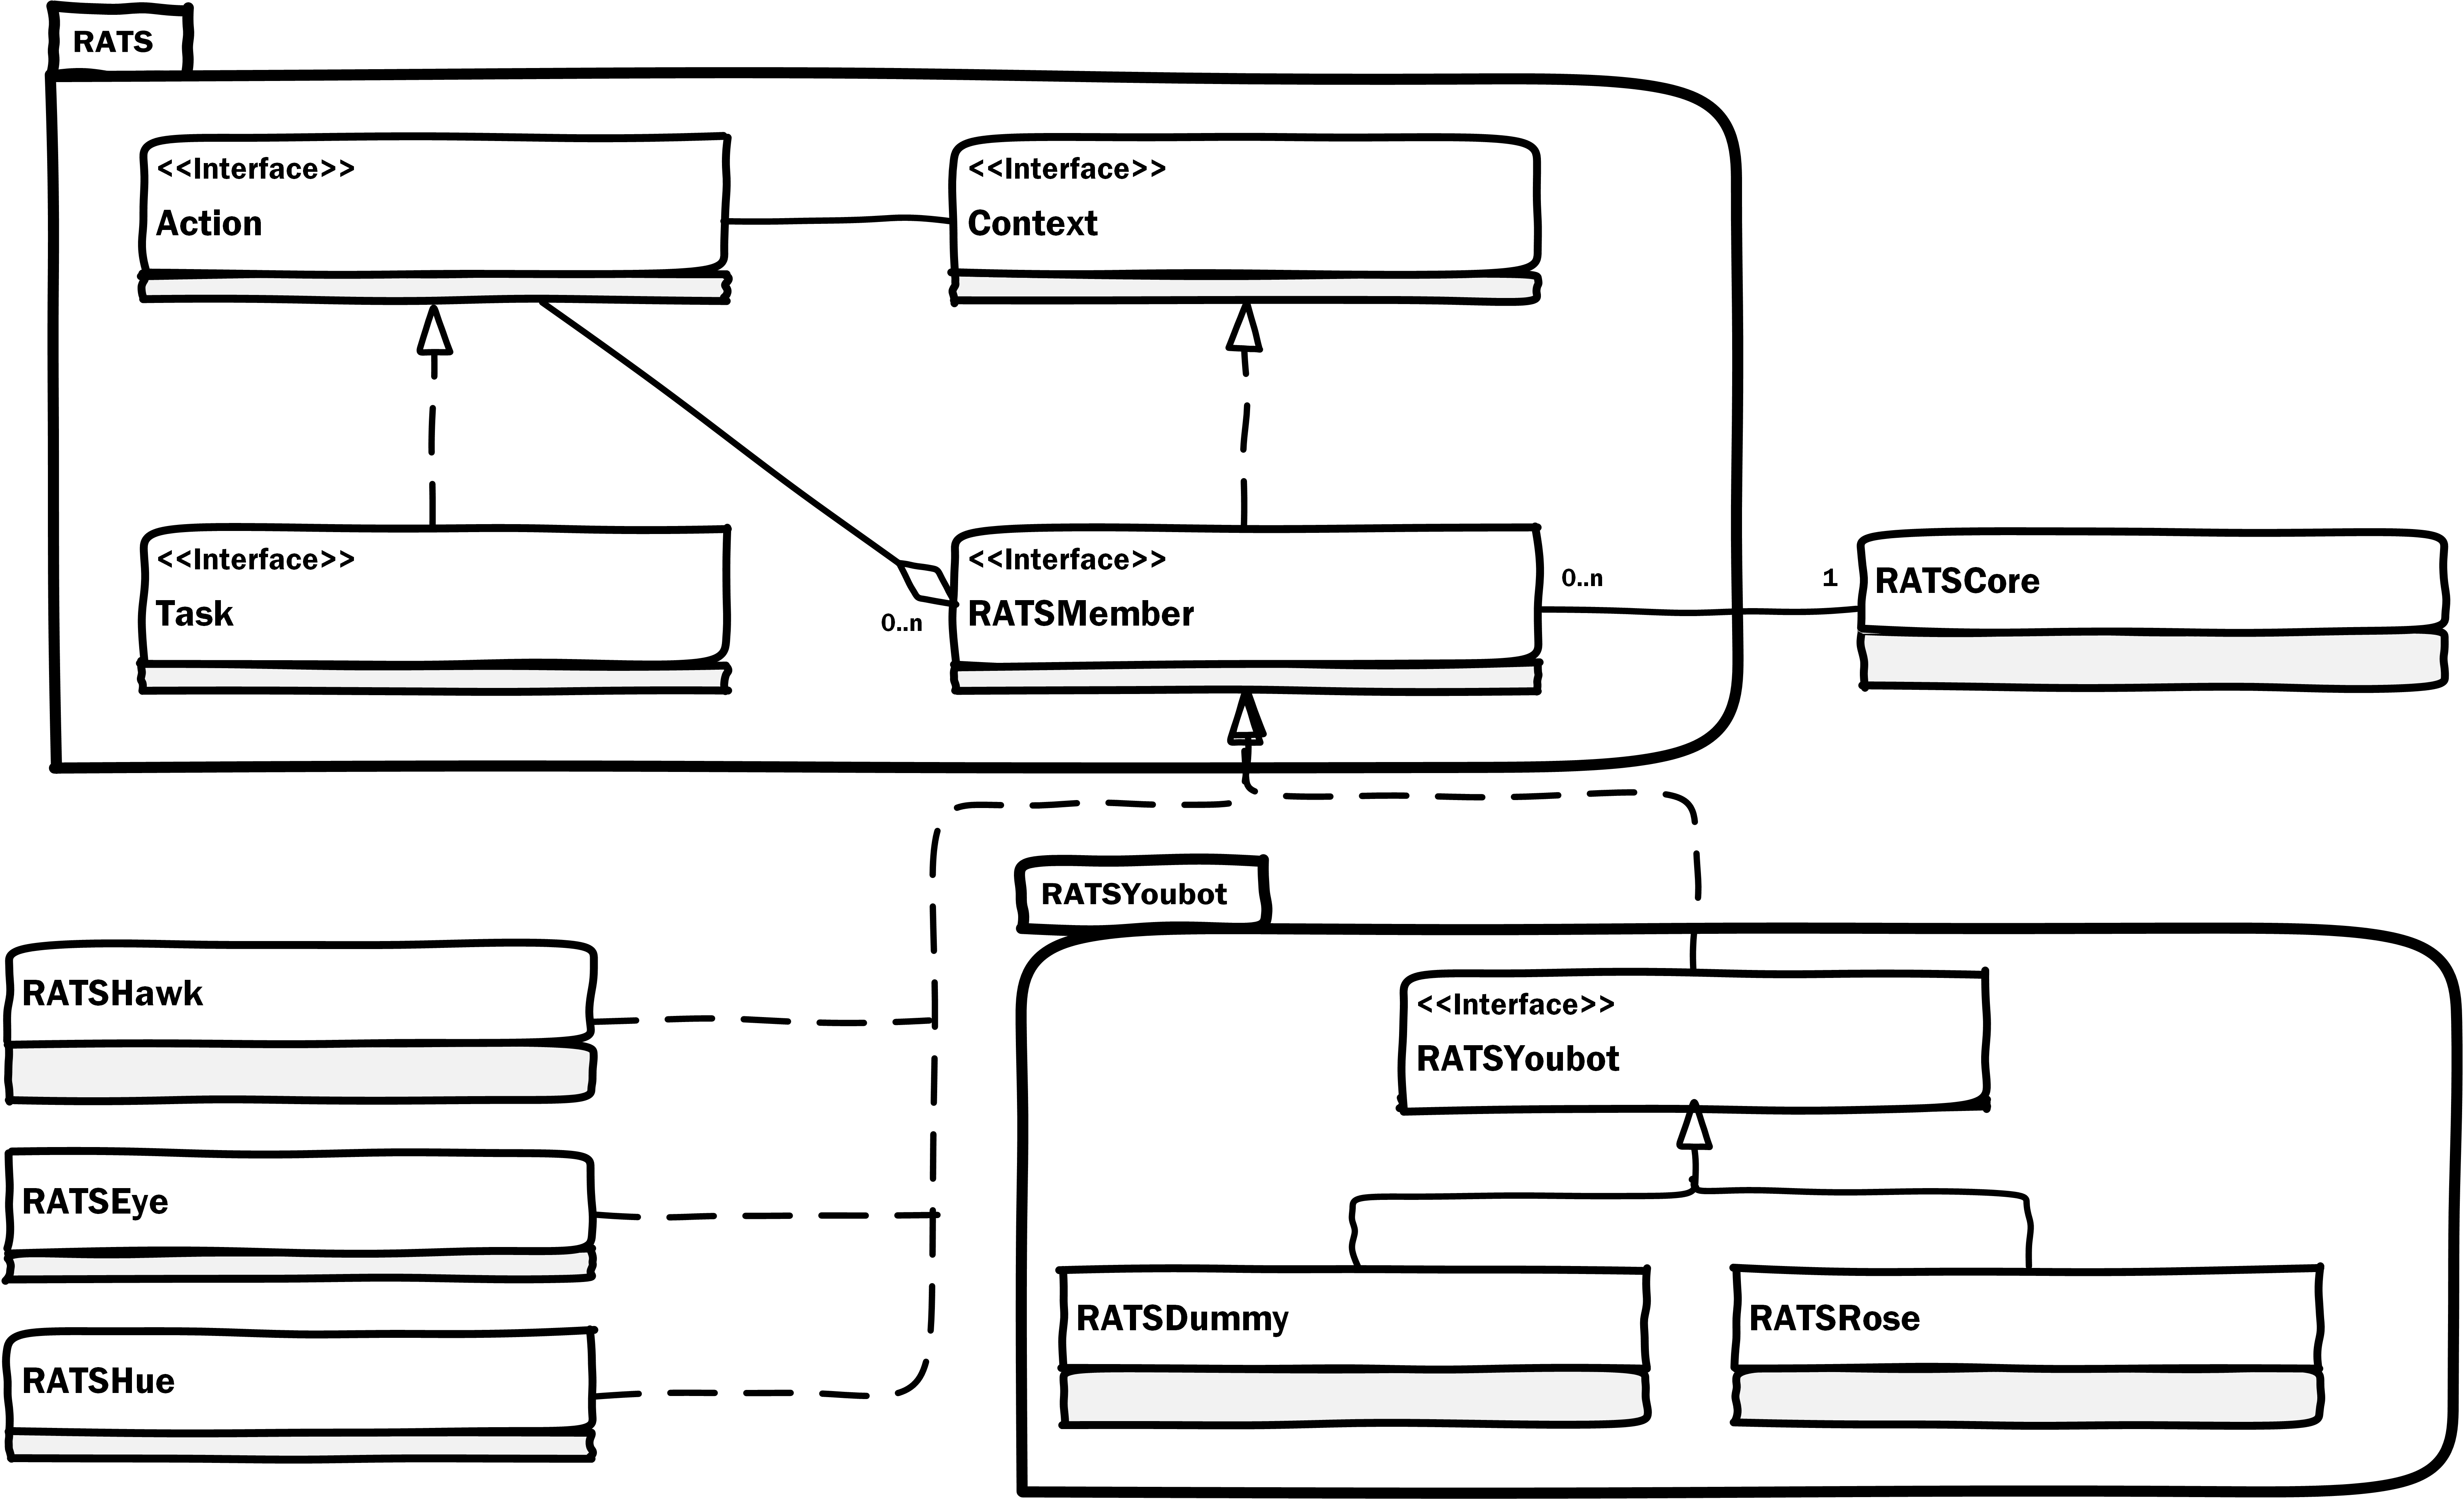
\includegraphics[scale=0.5]{fig/classrats}
	\caption[Klassenübersicht RATS]{Klassendiagramm RATS in der Übersicht. Die zentrale Komponente ist das RATS Paket. Dieses definiert die Schnittstellen Action, Task und RATSMember. Der MRS Controller RATSCore gehört nicht zum RATS Paket, da er je nach Konfigurations- und Koordinierungsaufwand unterschiedlich implementiert werden kann. Das Paket RATSYoubot implementiert die RATSMember von Rosie und Dummy. Alle anderen Sensoren und Aktoren implementieren die RATSMember Schnittstelle und sind jeweils in eigenen Paketen organisiert.}
	\label{fig:classrats}
\end{figure}


Als Grundlage für die Architektur liegt das Strategy Entwicklungsmuster. Dabei stellt die Action, beziehungsweise der Task, die Strategy und die RATSMember den Kontext dar. Soll eine Action ausgeführt werden wird, lädt der RATSMember die Action. Dazu wird zunächst der aktuelle Kontext an die Action übergeben. Dieser Kontext beinhaltet mögliche Parameter die benötigt werden. Dabei wird zwischen lokalen und globalen Kontext unterschieden. Der lokale ist nur während der Ausführung der Task oder Action verfügbar und wird anschließend gelöscht. Der globale Kontext ist Action und Agent übergreifend. Er kann dazu genutzt werden Umweltinformationen abzubilden und Allgemein verfügbar zu machen. Dieses Konzept ist dem PEIS-Konzept mit seinem Tupelförmigen Speicher angeglichen (siehe Kapitel \ref{sec:peis-imple}). Nach der Zuweisung des Kontext wird die \lstinline|execute()|-Methode der Action aufgerufen. Diese führt die gewünschte Funktionalität aus. Dabei kann der Kontext geändert werden. Dies ist vor allem bei Sensoren nötig, da diese ihre Daten nicht über einen Rückgabewert an den Aufrufer zurückgeben, sondern die Daten in den globalen Kontext schreiben. Ein Eingabeparameter dient dabei als Pfad für den Speicher. Ein Beispiel ist in Abbildung \ref{fig:seqspeicher} dargestellt. Dieses zeigt ein Sequenzdiagramm zur Anwendung des globalen Speichers. Leere Antworten wurden zur Übersichtlichkeit ausgelassen. Der Anwender setzt einen Befehl an den Core. Dieser Befehl beinhaltet einen Farbwert-Parameter, der der Oberflächenfarbe eines Objektes entspricht. Dieser Parameter wird unter einem Objekt mit der ID \textit{objid} abgelegt. Anschließend wird ein Sensor aktiviert, der das Objekt finden soll. Bei der Aktivierung wird der Objektpfad für den Speicher übergeben. Der Sensor holt sich die Daten aus dem globalen Speicher, lokalisiert das Objekt und schreibt die Position in den Speicher unter den selben Objektpfad zurück. Im Speicher liegen nun die Daten zu Farbe und Position des Objektes. Nach der Lokalisierung wird an einen Aktor der Befehl zur Aufnahme gesendet. Als Parameter wird nur die Objektid übergeben. Der Aktor lädt die zuvor gesammelten Daten aus dem Speicher und hebt das Objekt an der übermittelten Position auf.

\begin{figure}
	\centering
	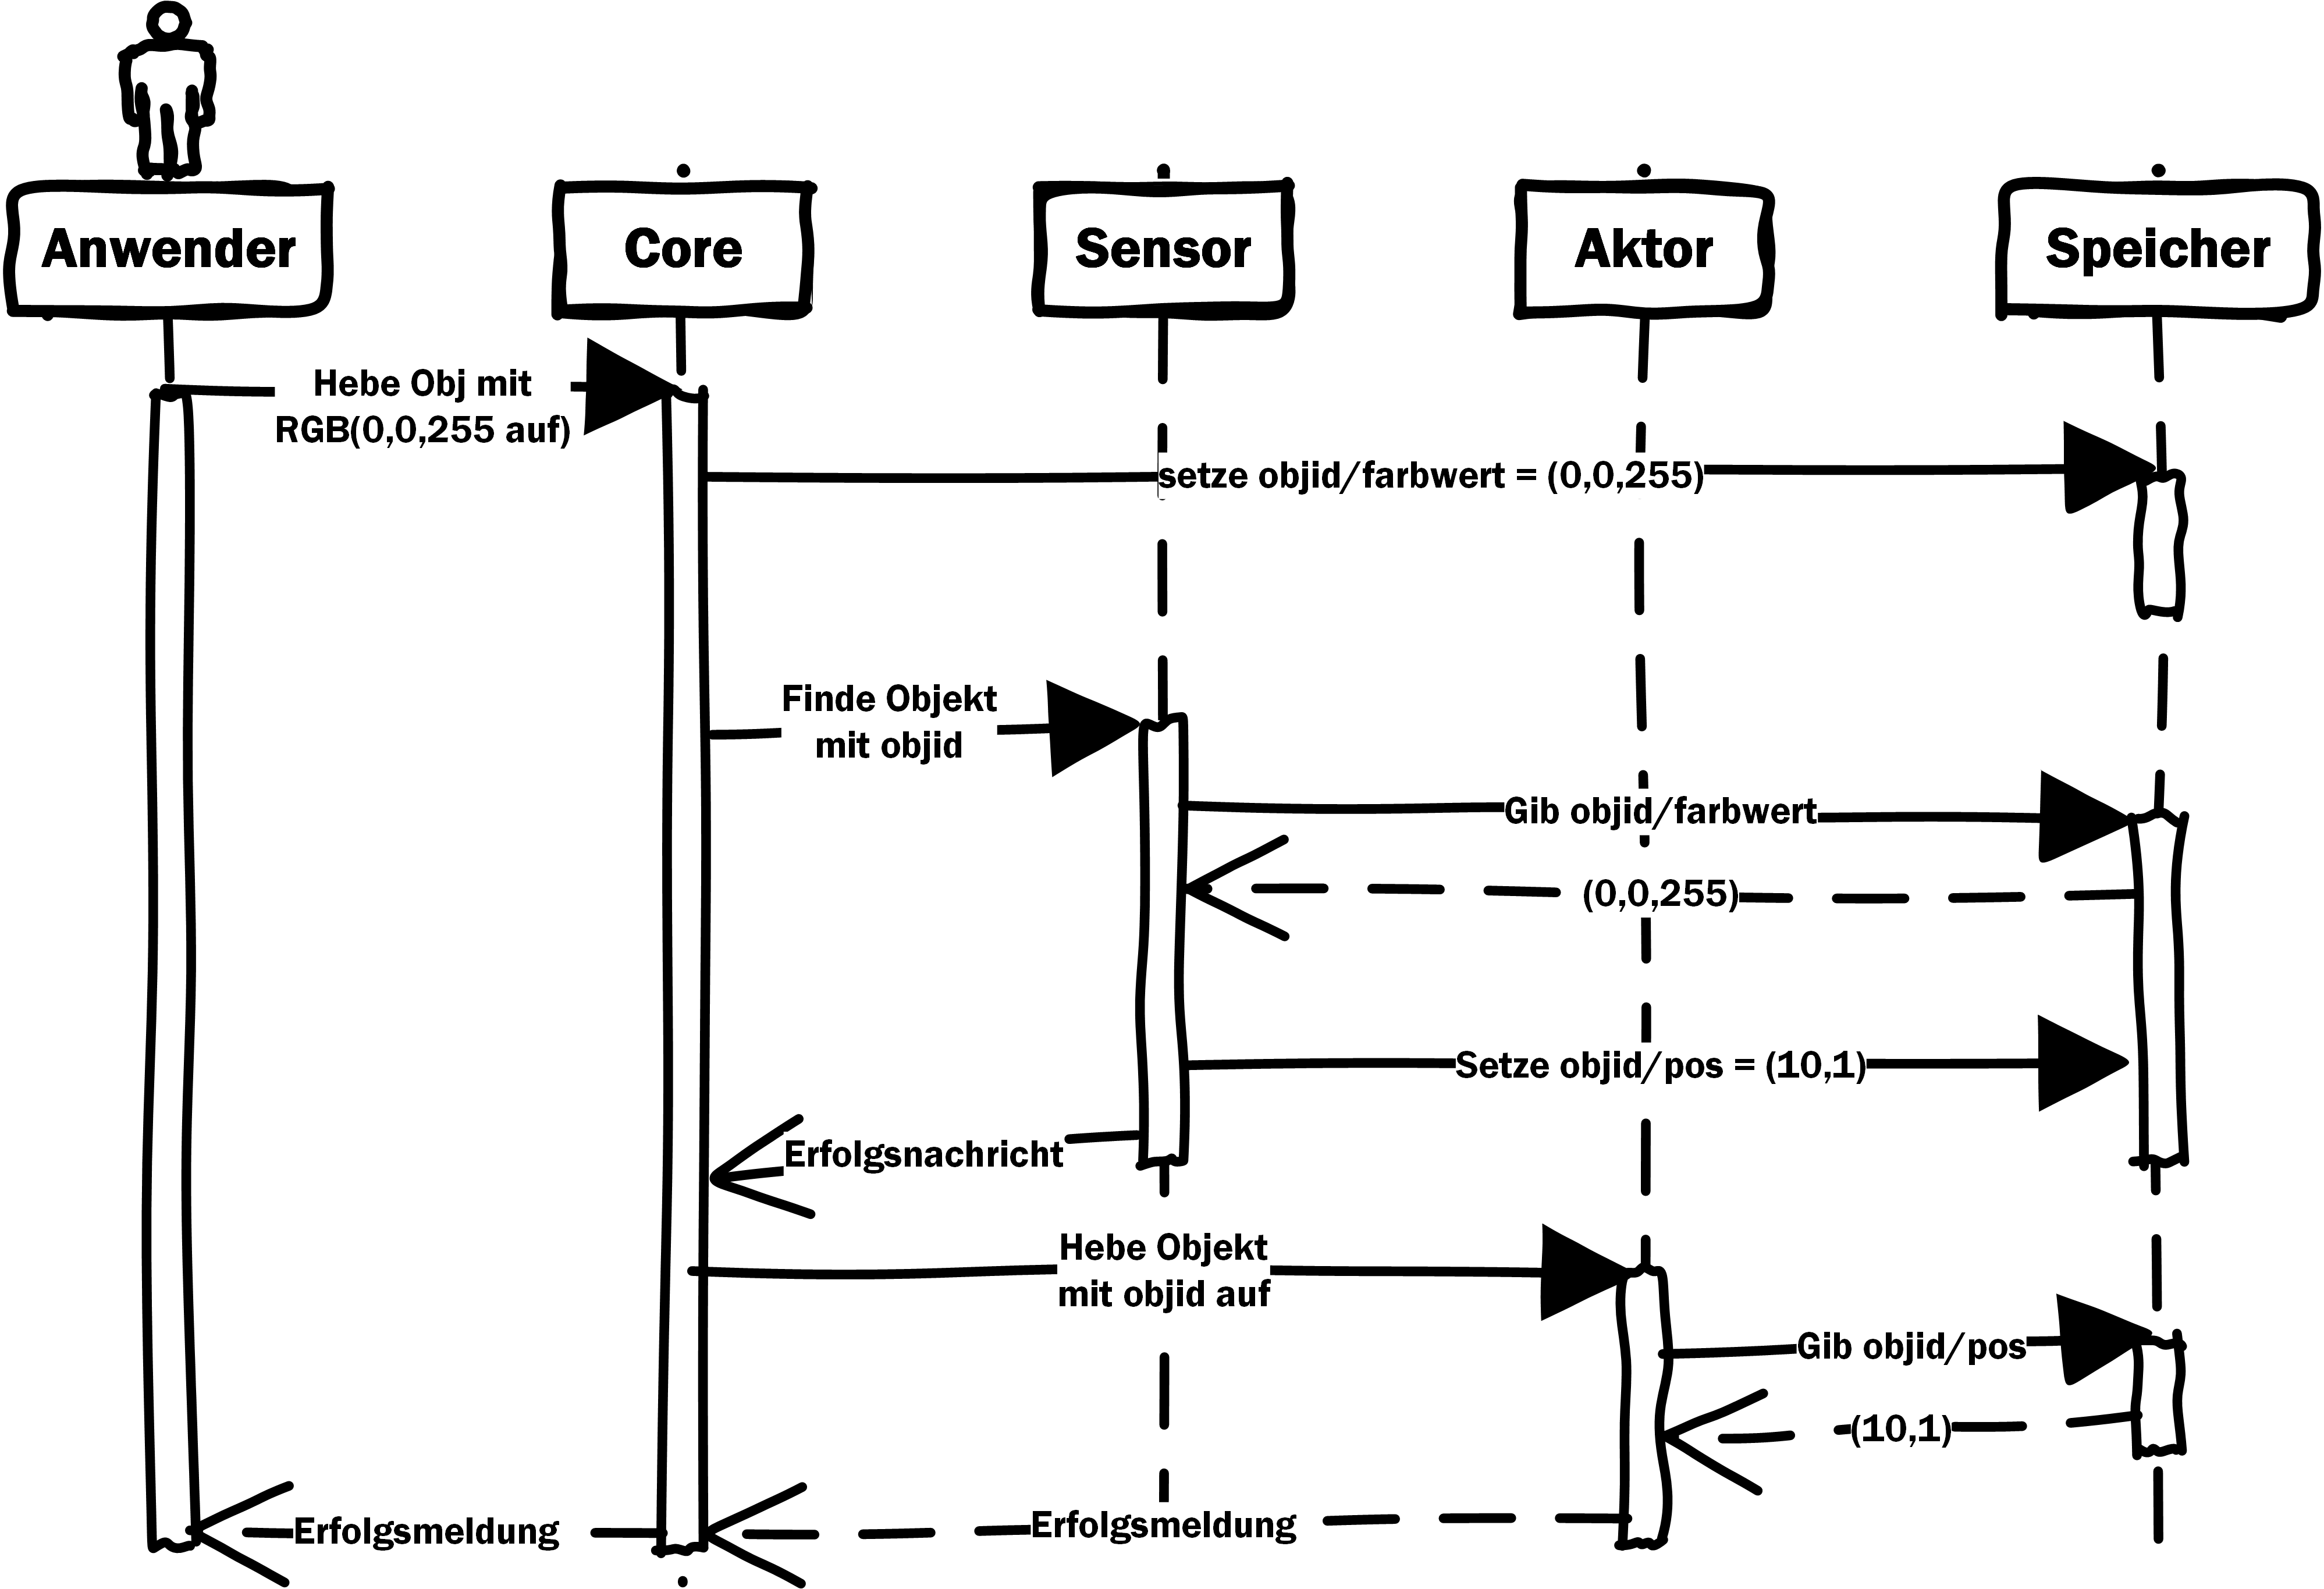
\includegraphics[scale=1.0]{fig/seqspeicher}
	\caption[RATS globaler Speicher]{Beispielhaftes Sequenzdiagramm zur Erklärung vom globalen Speichersystem. Zur Vereinfachung ist ein Erfolgsmeldung dargestellt und leere Antworten wurden entfernt.}
	\label{fig:seqspeicher}
\end{figure}

\subsubsection{RATSAction und RATSTask}
RATSAction und RATSTask bilden die Funktionalitäten innerhalb der Architektur ab. Wie im Konzept beschrieben werden sie von außen angestoßen und durch den Agenten eingesetzt. Damit die Aktion oder der Task erreichbar ist, kann sie über eine ID erreicht werden. Die ID steht dabei für eine Funktionalität des MRS. Eine Funktionalität kann von verschiedenen Agenten unterschiedlich implementiert werden. Sie wird dann als Action oder Task mit der dazugehörigen ID publiziert. Dieses Konzept folgt der Definition aus Kapitel \ref{sec:dev-funk}. Außerdem kann jede Action, einschließlich Tasks, den aktuellen Zustand des Systems ändern. Dies geschieht über den globalen Speicher. 

Die zentrale Methode jeder Action ist  \lstinline|execute()|-Methode. Diese besitzt die Logik der Action und ist immer gleich aufgebaut. Zuerst wird der lokale Kontext ausgelesen. In diesem befinden sich mögliche Zeiger auf den globalen Speicher. Dieser wird darauf ausgelesen. Darauf folgt eine Überprüfung, ob alle benötigten Eingabeparameter vorhanden und gültig sind. Dies betrifft auch den aktuellen Systemzustand. Ist diese Überprüfung ungültig bricht die Funktion mit einer Fehlermeldung ab. Anschließend folgt die Ausführung der Funktion. Auch hier wird bei einer Fehlfunktion eine Rückmeldung gegeben und die weitere Ausführung abgebrochen. Zum Abschluss schreibt die Action zunächst Ergebnisse in den globalen und dann in den lokalen Kontext. Neben der Ausführung besitzt jede Action eine Methode die Kosten für eine Funktion vor zu berechnen. Dabei ist die Kostenfunktion von der Funktion und den Umweltparametern abhängig. Diese Methode wurde für eine automatische Konfiguration vorgesehen. So werden die Actions mit ihrer Funktion-ID und den Umweltparametern, im globalen Speicher, angeboten. Alle Agenten, die eine Action mit dieser ID haben, können nun die Kosten ermitteln und mit diesen bieten. Dabei gewinnt der Agent mit den geringsten Kosten. Die Kostenfunktion greift nur lesend auf den Speicher zu und führt die Aktion auch nicht aus.

RATSTasks bieten die Möglichkeit Actions miteinander zu verbinden. Dabei sind die Tasks selber Actions und können so ineinander verkettet werden. Der einfachste Task ist eine serielle Ausführung der hinterlegten Actions. Bricht eine Action ab, bricht der ganze Task ab. Komplexere Tasks steuern parallele oder bedingte Ausführungen von Actions. Dabei können Fehler abgefangen und behandelt werden. So ermöglicht ein Task, dass ein Roboterarm nach einem Fehlschlag der Action in einen sicheren Zustand (Candle- oder Fold-Pose) wechselt.


\subsubsection{RATSMember}
Die RATSMember repräsentieren die Agenten im MRS. Jeder RATSMember registriert sich bei der zentralen Komponente, dem RATSCore, mit einer eindeutigen ID. Ist diese ID im System schon vergeben, beendet sich der Agent und es muss eine neue ID vorgegeben werden. Unter dieser ID kann der Agent im MRS erreicht werden. Neben der ID besitzt jeder RATSMember eine Menge an Tasks und Actions die von diesem ausgeführt werden können. Diese Menge übersendet der RATSMember bei der Registrierung an den RATSCore. 

Da ROS als Grundlage für diese Arbeit dient, tritt jeder RATSMember als selbstständiger ROS-Node auf. Dies dient vor allem zur Stabilisierung und Wiederherstellbarkeit des Systems. Die ROS Node-ID von einem RATSMember-Node wird auch als ID des RATSMember genutzt. Dadurch kann innerhalb eines MRS die Eindeutigkeit der ID gewährleistet werden. Damit ein RATSMember eine Action ausführt wird, muss der Member eine Nachricht mit der Action-ID und den Parametern erhalten. Zunächst war für diese Kommunikation ein ROS-Topic angedacht, wie im PEIS Konzept vorgesehen (siehe Kapitel \ref{sec:peis-imple}). Nach der Entwicklung eines ersten Prototypen zeigte sich jedoch, dass diese Methodik Nachteile bringt. So kann ein Publisher an einem ROS-Topic nicht sicherstellen, ob ein Subscriber die Nachricht erhalten hat. Außerdem ermöglichen Topics keine Rückgabewerte. Deshalb wurde für die weitere Entwicklung die Action-Lib von ROS (siehe \ref{sec:basic-ros-action}) genutzt. Diese ermöglicht einen RPC ähnlichen Aufruf. Gegenüber den Services von ROS können außerdem Zwischenergebnisse zurückgegeben werden. Dies ermöglicht eine Schnittstelle für komplexere MR-Tasks mit hohem Koordinierungsaufwand. Ein Problem stellen die dynamischen Parameterlisten dar. Diese sind für das System nötig, da je nach Koordinierungsaufwand unterschiedlich viele Daten mit variablem Datentypen übergeben werden muss. Die Action-Lib, wie auch Services und Topics, lassen keine dynamischen Parameterlisten innerhalb ihrer Messages zu. Darum werden diese Nachrichtenparameter als Strings definiert. Der Inhalt dieser Strings sind JSON-Objekte. Der Aufbau der JSON Objekte ist in Abbildung \ref{fig:jsonmsg} dargestellt. Das Root-Element besteht aus dem Objekt Header und dem Array der dynamischen Parameterliste. Der Header wird nur in der Kommunikationsschicht ausgewertet und beinhaltet die Agent- und die Action-ID. Die Parameterliste wird vom RATSMember geparst und dem lokalen Kontext hinzugefügt. Nach Ausführung der RATSAction wird aus dem lokalen Kontext ein JSON-Objekt erstellt, welches anschließend als Rückgabewert in der Message gesendet wird. Sollte eine RATSAction fehlschlagen wird in den Header ein Fehlercode eingetragen, der vom Aufrufer ausgewertet wird. Als JSON-API kommt die RapidJSON Bibliothek zum Einsatz.

\begin{figure}
	\centering
	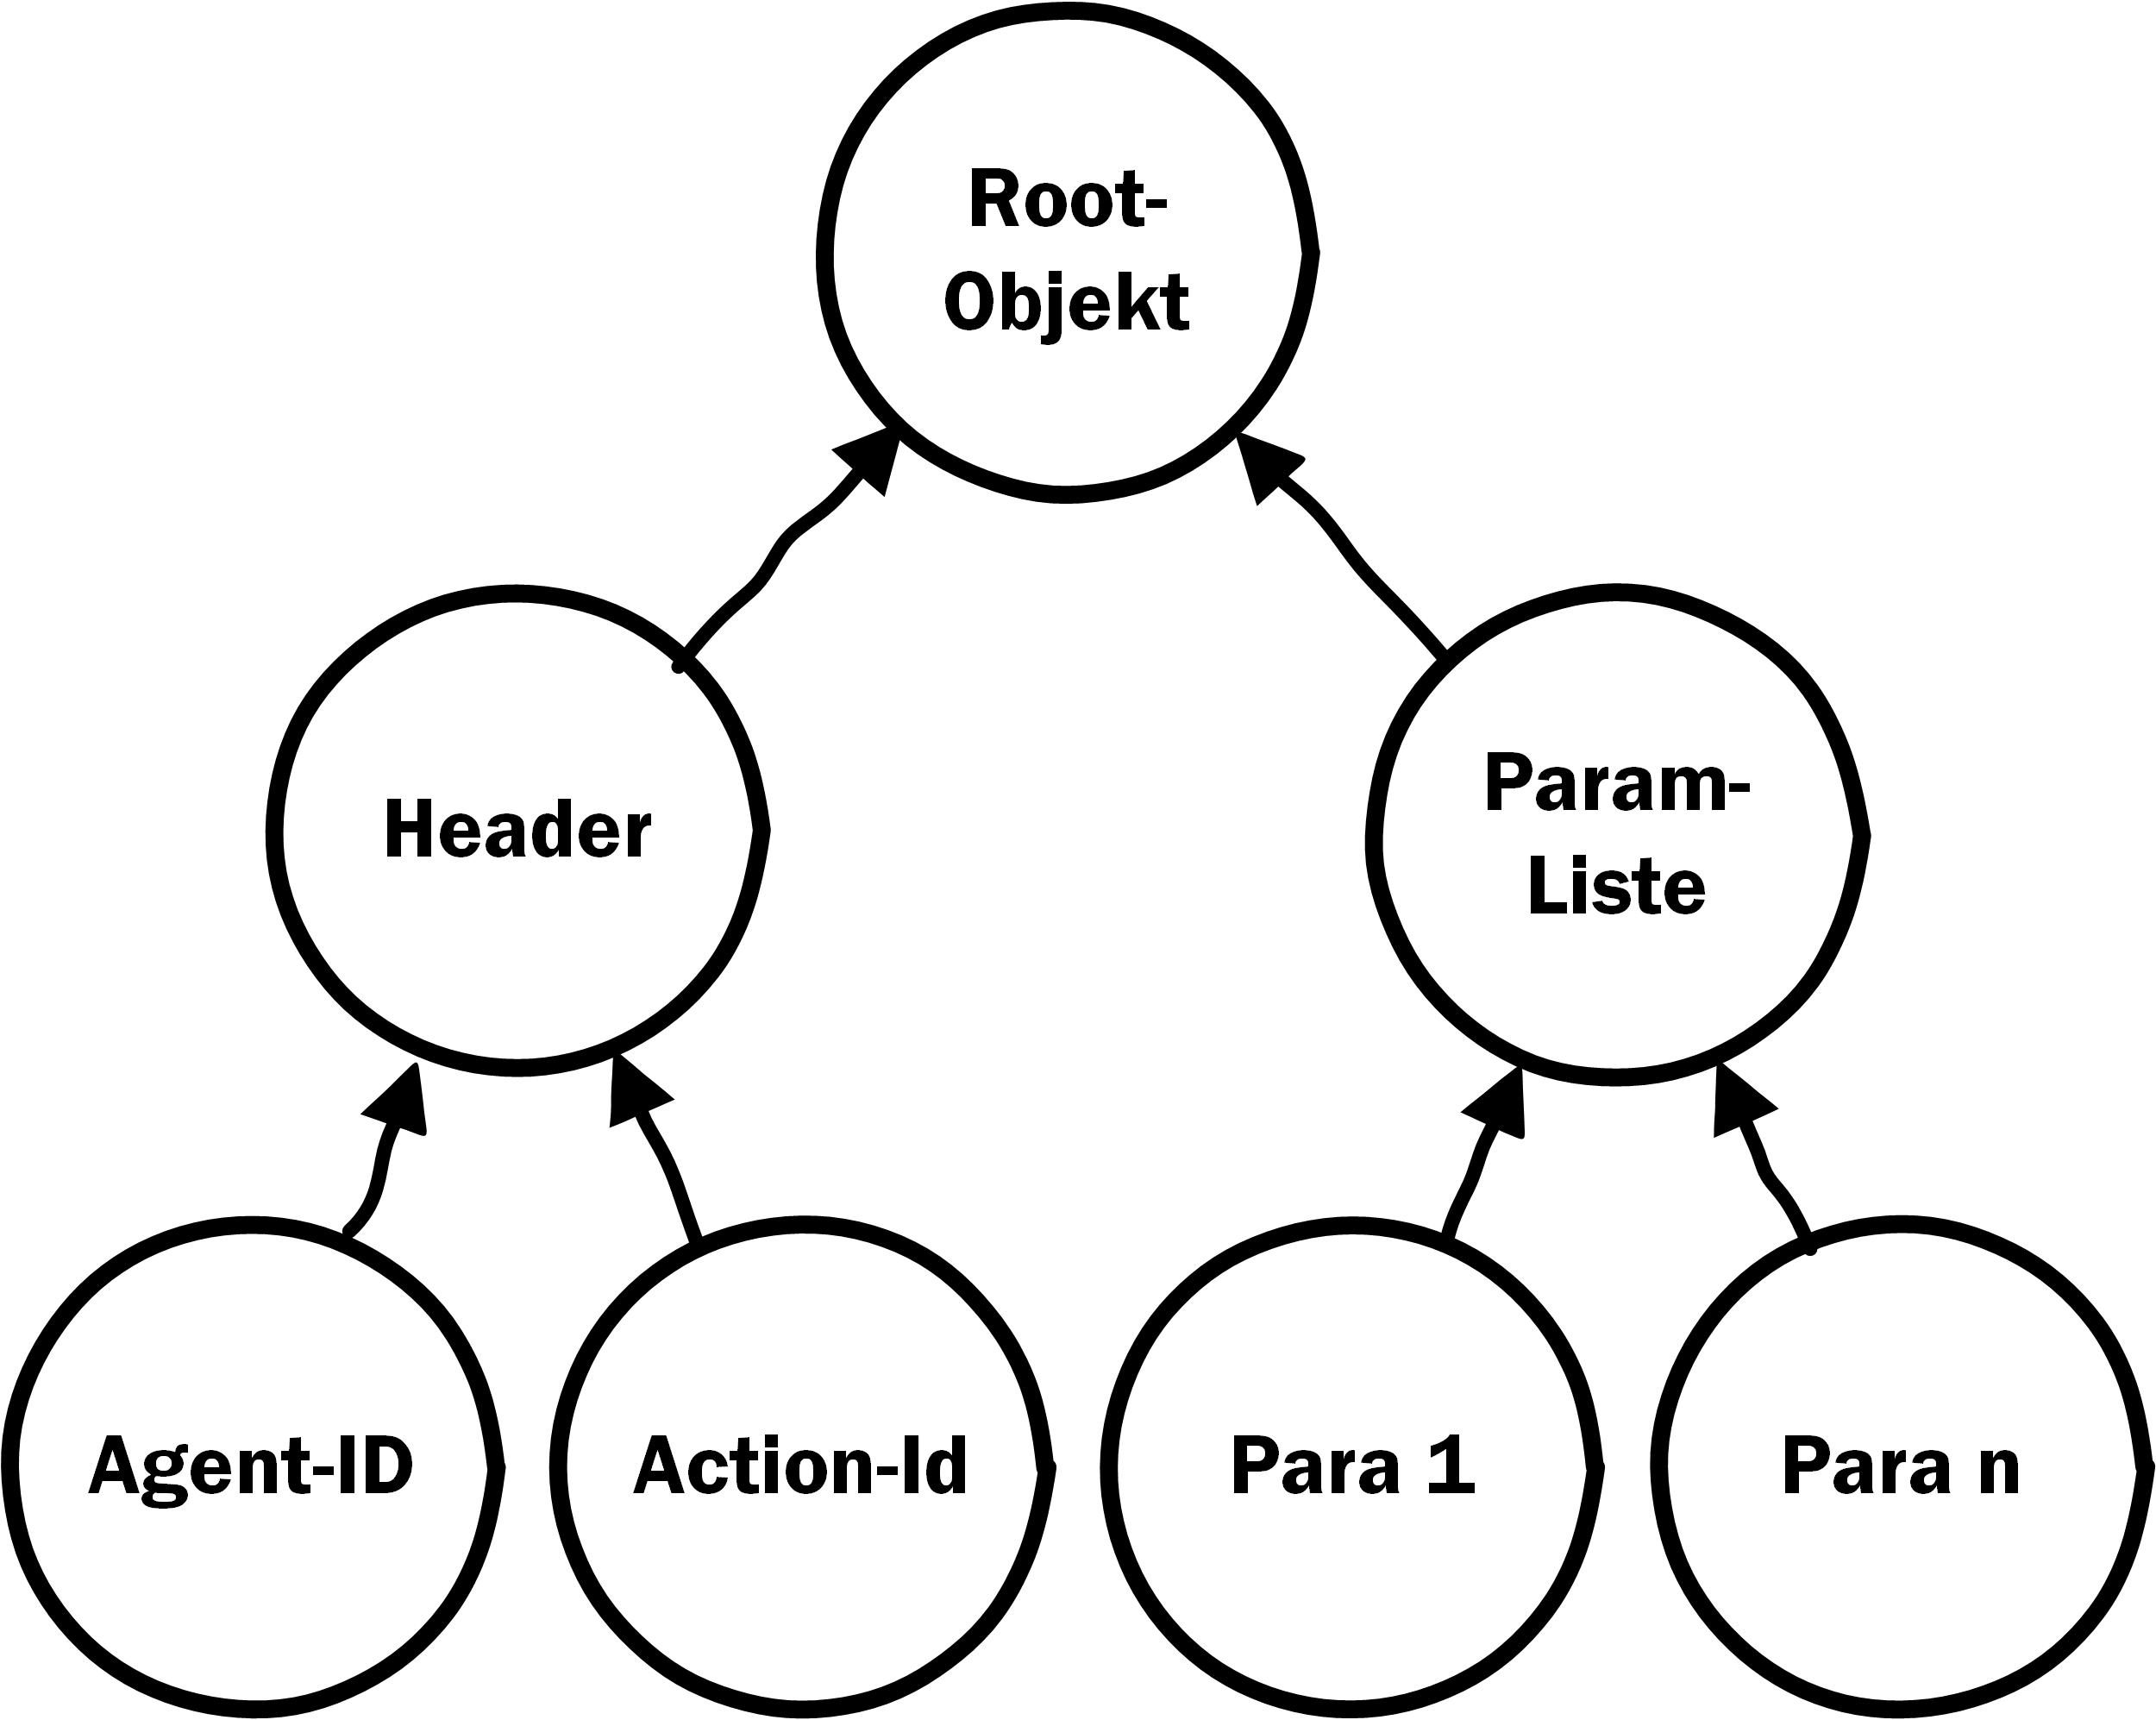
\includegraphics[scale=1.0]{fig/jsonmsg}
	\caption[JSON Action Message]{Aufbau einer JSON Action Message. Unter dem Root-Element hängen der Header und die Parameter-Liste. Der Header beinhalten Informationen über die Agent-ID und die Action-ID. Die Parameter-Liste enthält den dynamischen lokalen Kontext.}
	\label{fig:jsonmsg}
\end{figure}

\subsubsection{RATSCore}
Der RATSCore ist der zentrale Koordinierungs- und Konfigurationscontroller. An diesem melden sich alle RATSMember an und ab. Des Weiteren bietet der RATSCore Schnittstellen für Steuerungsoberflächen. Für diese Arbeit wird eine einfache Konsole umgesetzt, aus der die gewünschten Actions und Tasks  gestartet werden können. Es sind aber auch eine andere Ansteuerung, wie Sprach- oder Gestensteuerung realisierbar. Die Konfigurations- und Koordinierungsaufgaben werden in dieser Arbeit mit Hilfe von Textdateien vorgegeben. Dabei wird die Agenten-ID, die Action-ID und die nötigen Parameter, zum Beispiel Zeiger auf den globalen Speicher, angegeben. Diese Textdateien werden von dem Core zur Laufzeit eingelesen. Der Core übernimmt dann die Ansteuerung und Verwaltung der RATSMember.

Der RATSCore ist ein selbstständiger ROS-Node, der mit dem ROS Core zusammen gestartet wird. Da er eine zentrale Komponente darstellt ist er ein potenzieller Single-Point-of-Failure. Fällt er aus bricht das System zusammen. Je nach Systemzustand kann dies zu weiteren Problemen führen. Damit dies abgesichert ist, sind Sicherheitsmechanismen in die unterschiedlichen Kommunikationsschichten eingebaut. So brechen RATSMember ihre Aktionen im Ausfall nicht ab, sondern führen diese bis zum Ende aus. Können sie dann keine Rückmeldung an den RATSCore senden gehen die RATSMember in einen sicheren Zustand über. Dies betrifft besonders mechanische Aktoren, wie die Roboterarme. Bekommt der Core keine Rückmeldung mehr von einem RATSMember nach einer bestimmten Zeit, so bricht er die gesamte Aufgabe ab. Meldet sich ein RATSMember im Ruhezustand ab, werden seine Actions und Tasks aus dem Speicher genommen, so wird er bei zukünftigen Aufgaben nicht mit eingeplant. Dadurch sichert die RATSCore einen sicheren Systemzustand. Ist ein RATSCore einmal abgestürzt müssen auch alle Member einmal neu gestartet werden. Dadurch registrieren sie sich neu an dem RATSCore.

\subsection{Inverse Kinematik}
In diesem Kapitel wird die Entwicklung der inversen Kinematik vorgestellt. Dabei wird zunächst auf die schon existierenden inversen Kinematiken für den YouBot Arm eingegangen und eine Bewertung dieser vorgenommen. Darauf folgt die Entwicklung eines stark vereinfachten Prototypens, dessen Weiterentwicklung die endgültige inverse Kinematik darstellt. Den Abschluss bildet die Optimierung der Lösungen der inversen Kinematik mit Bezug auf die Pfadfindung.

\subsubsection{YouBot Kinematiken}
Mit dem YouBot wird bereits das Software-Paket \textit{MoveIt!} zur Bewegungs- und Pfadbestimmung mitgeliefert. Es ist ROS-basiert und nutzt zur Visualisierung und Konfiguration ein RViz-Plugin. Die implementierte Pfadbestimmung verwendet numerische Ansätze für das Lösen der Bewegungsbahnen. Dabei stehen folgende Planungsbibliotheken zur Auswahl: Die \textit{Open Motion Planning Library} (OMPL), \textit{Covariant Hamiltonian Optimization and Motion Planning} (CHOMP) und \textit{Search-based planning} (SBPL). Die OMPL beinhaltet verschiedene Algorithmen zur Bewegungsplanung die alle auf abstrakten Zuständen des Systems beruhen. Dabei wird zwischen probabilistischen (PRM) und Baum-basierten Algorithmen (RRT, EST, KPiece, SBL) unterschieden. Alle Algorithmen lassen sich konfigurieren, dies betrifft vor allem die Anzahl der Iterationen und die Zeitschranke für die Dauer der Berechnung. Für diese Arbeit wurden drei verschiedene Algorithmen (PRM, EST, CHOMP) für eine Bewertung ausgewählt und evaluiert. Bei dieser Evaluierung wurden fünf Bewegungsziele abgesteckt, welche vom Roboter angefahren werden sollte. Die Anzahl der Iterationen wurden in drei Messgruppen (zehn, 100 und 1000 Iterationen) aufgeteilt und mit jedem Algorithmus getestet. Die Zeitschranke wurde auf 30 Sekunden eingestellt, um möglichst gute Messungen zu erreichen. Pro Bewegungsziel wurde die Dauer der Planung $t$ in Sekunden und die Genauigkeit der Endpose in Zentimetern und Grad gemessen. Dabei wurden die euklidische Distanz für den linearen und dem rotierenden ermittelt: 

\begin{math}
\delta_{lin} = \|\lambda(\xi_{Ziel}) - \lambda(\xi_{Plan})\|_2 = \sqrt{\sum_{i=1}^{3}(\xi_{Ziel,i}-\xi_{Plan,i})^2}	
\end{math}

\begin{math}
	\delta_{rot} = \|\theta(\xi_{Ziel}) - \theta(\xi_{Plan})\|_2 = \sqrt{\sum_{i=4}^{6}(\xi_{Ziel,i}-\xi_{Plan,i})^2}
\end{math}

Wobei die $\lambda$-Funktion den linearen und die $\theta$-Funktion den rotierenden Anteil der Pose Für jedes Bewegungsziel setzt sich so ein Bewertungsvektor zusammen mit $x \in  \mathbb{R}^3$:

\begin{math}
x = \left(\begin{array}{c} t \\ \delta_{lin} \\ \delta_{rot} \end{array}\right)	
\end{math}

Diese Ergebnisse wurden gemittelt und in Tabelle \ref{tab:mesplan} eingetragen.
\begin{table}
	\caption[Gemittelte Messwerte der MoveIt!-Planer-Algorithmen]{Die gemittelten Messwerte der MoveIt!-Planer. In den Zeilen sind die unterschiedlichen Interationen pro Planung gegeben. Die Spalten geben den verwendeten Planer-Algorithmus an. Die Messwerte $x$ setzen sich aus der benötigten Planungszeit $x_1$ und der euklidischen Distanz der Zielpose zur Planpose zusammen. Dabei wird zwischen linearer $x_2$ und rotierender $x_3$ Distanz unterschieden.}
	
	\centering
	\begin{tabular}{|c|c|c|c|}
		\hline  	& PRM & EST & CHOMP \\ 
		\hline 10 	&  &  &  \\ 
		\hline 100 	&  &  &  \\ 
		\hline 1000 &  &  &  \\ 
		\hline 
	\end{tabular}
	
	\label{tab:mesplan}
\end{table}
	

\clearpage
%%%%%%%%%%%%%%%%%%%%%%%%%%%%%%%%%%%%%%%%%%%%%%%%%%%%%%%%%%%%%%%%%%%%%%%
%% Zusammenfassung und Ausblick
\section{Implementierung}
\label{sec:impl}

In diesem Kapitel werden einige Aspekte der Entwicklung aufgegriffen und im Detail ausgeführt. Der Name Implementierung bezieht sich nicht auf die Programmierung, sondern die Umsetzung von Schnittstellen und den Algorithmen hinter speziellen Problemen. So wird zum Beispiel in dem Unterkapitel \ref{sec:impl-rs} auf die Bewegung auf einer linearen Trajektorie eingegangen. Außerdem werden Probleme beschrieben und gelöst, die während der Umsetzung der Konzepte auftraten. Des Weiteren werden die genutzten Bibliotheken erwähnt und die Anbindung von ROS an die Konzepte. Den zentralen Aspekt in diesem Kapitel stellt jedoch Unterkapitel \ref{sec:impl-hop} dar. In diesem wird die Bestimmung für die Übergabeposition vorgestellt.

\subsection{Robotersteuerung - RATSYoubot \& RATSDummy \& RATSRose}
\label{sec:impl-rs}
In diesem Kapitel wird die Ansteuerung für die Roboter und deren Arme vorgestellt. Diese beruht vor allem auf der Kuka API für den Youbot. Außerdem wird die Bewegung auf einer linearen Trajektorie, sowie die einzelnen Aktionen die ein Roboter ausführen kann kurz aufgelistet und beschrieben.

\subsubsection{Ansteuerung der Aktoren}
\label{sec:impl-res-ak}
Die Aktoren innerhalb der Roboter werden mit Hilfe von ROS Topics angesteuert. Diese werden von dem Controllernode \textit{youbot\_driver} ausgelesen und in die Steuersignale für die Motoren umgewandelt. Für die Ansteuerung des Arms existieren zwei Topics. Der \textit{velocity\_command}-Topic erwartet für jedes Gelenk eine Geschwindigkeitsangabe. Für diese Arbeit wird jedoch mit Positionsangaben gearbeitet. Der dazu gehörige Topic \textit{arm\_controller/position\_command} benötigt ein Array mit Gelenkkonfigurationen. Dafür wird die ROS-Bibliothek \textit{BRICS} genutzt. Diese beinhaltet Nachrichten für inverse Kinematiken, wie zum  Beispiel: Posen, Vektoren und Rotationen im Kartesischen Raum oder Aktoren Nachrichten, wie Gelenkeinstellung, Gelenkgeschwindigkeiten und Gelenkbeschleunigungen. Neben der Armansteuerung gibt es für die Gripper eine eigene Topic \textit{gripper\_controller/position\_command}. Dieser transportiert ebenfalls Gelenkeinstellungen. Dabei kann die Position der einzelnen Finger des Grippers angegeben werden. Die Werte entsprechen dabei der Distanz der Finger zu ihrer Basisposition. Ein Nachteil der Ansteuerung über die Topics ist das fehlende Feedback. Der Absender erfährt nicht, ob das Signal angekommen ist und wann die Bewegung beendet ist. Sollen Bewegungen seriell ausgeführt werden muss der ausführende Thread blockiert werden, bis die Gelenke die Zielkonfiguration erreicht haben.  Ein paralleler Thread liest die aktuelle Gelenkkonfiguration aus und berechnet eine Differenz für jedes einzelne Gelenk und die Quadratsumme über alle Gelenke. Solange die Differenz für mindestens ein Gelenk oder die Summe der Quadrate ihre Schwellwerte überschreiten blockiert ein Mutex den ausführenden Thread. Ein weiteres Problem während der Implementierung stellte die Ungenauigkeit der Ansteuerung dar. Dabei kam es großen Abweichungen an einem Gelenk, wenn es eine große Winkeländerung hatte. Dieses Überschlagen lässt sich auf die Massenträgheit des Armes und dem abrupten Abbremsen der Motoren zurückführen. Dies konnte jedoch auch durch den parallelen Thread abgefangen werden. Dieser überprüft nun auch neben der Distanz zu der Zieleinstellung, die Distanz zur letzten gemessenen Gelenkeinstellung. Ist diese nahe null, also der Arm nicht mehr in Bewegung, und die Distanz zum Ziel zu groß wurde nochmal die selbe Gelenkeinstellung an den Motorencontroller geschickt.

Die Ansteuerung der mobilen Plattform wird mit einer einzelnen Topic \textit{cmd\_vel} umgesetzt. Dabei wird eine einzelne Nachricht übermittelt. Diese beinhaltet eine Twist Nachricht aus dem \textit{geometry\_msg} Paket. In dieser Nachricht kann eine lineare und eine Winkelgeschwindigkeit angegeben werden. Diese können für die einzelnen Achsen zerlegt werden. Für die mobile Plattform werden jedoch nur die X- und Y- Achsen der linearen, sowie die Z-Achse der Rotationsgeschwindigkeit ausgelesen und als absoluten Wert gesetzt. Der Controller rechnet anschließend die benötigten Steuersignale für die einzelnen Räder und Motoren aus.

\subsubsection{Lineare Bahnbewegung}
\label{sec:impl-res-lb}
Die lineare Bahnbewegung wird beim Aufheben, Ablegen und während der Übergabe benötigt. Dies liegt vor allem an der Kollisionsvermeidung des Objektes mit der Umwelt. Da die inverse Kinematik die Gelenkeinstellungen und nicht die Gelenkgeschwindigkeiten berechnet ist es nicht so einfach auf einer gezielten Trajektorie entlang zufahren. Der Übergang zwischen zwei Gelenkeinstellung wird nicht genau definiert. Wie in Abbildung \ref{fig:traj} dargestellt kommt es dabei durch unterschiedliche Gelenkgeschwindigkeiten zu einem Ausschlagen des Greifers. Je größer die Distanz zwischen zwei Posen, desto größer der Ausschlag. Deshalb kann dies verhindert beziehungsweise minimiert werden, indem Zwischenposen auf der Trajektorie ermittelt werden, die nacheinander angefahren werden. Dies erfordert zwar eine häufiges Aufrufen der inversen Kinematik, dafür kann eine Trajektorie mit einem geringen Ausschlag entlang gefahren werden. Tests mit dem YouBot Armen und der inversen Kinematik ergaben eine Distanz von 5 Millimetern zwischen den Zwischenposen als optimal. Bei einer kleineren Distanz reduzierte sich die Amplitude des Ausschlages weniger als vorher und steigert die Kosten durch einen häufigeren Aufruf der inversen Kinematik. Bei der Implementierung nutzt dafür vor allem die Orocos KDL Api, die auch bei der Implementierung der inversen Kinematik genutzt wird. Diese ermöglicht das Rechnen mit geometrischen Primitiven, so wurde der \lstinline|KDL::Frame| für die Abbildung von Koordinatensystemen und Posen genutzt. Dieser ermöglicht unter anderem die Bestimmung der Zwischenposen.

\begin{figure}[h]
	\centering
	\subfigure[]{%
		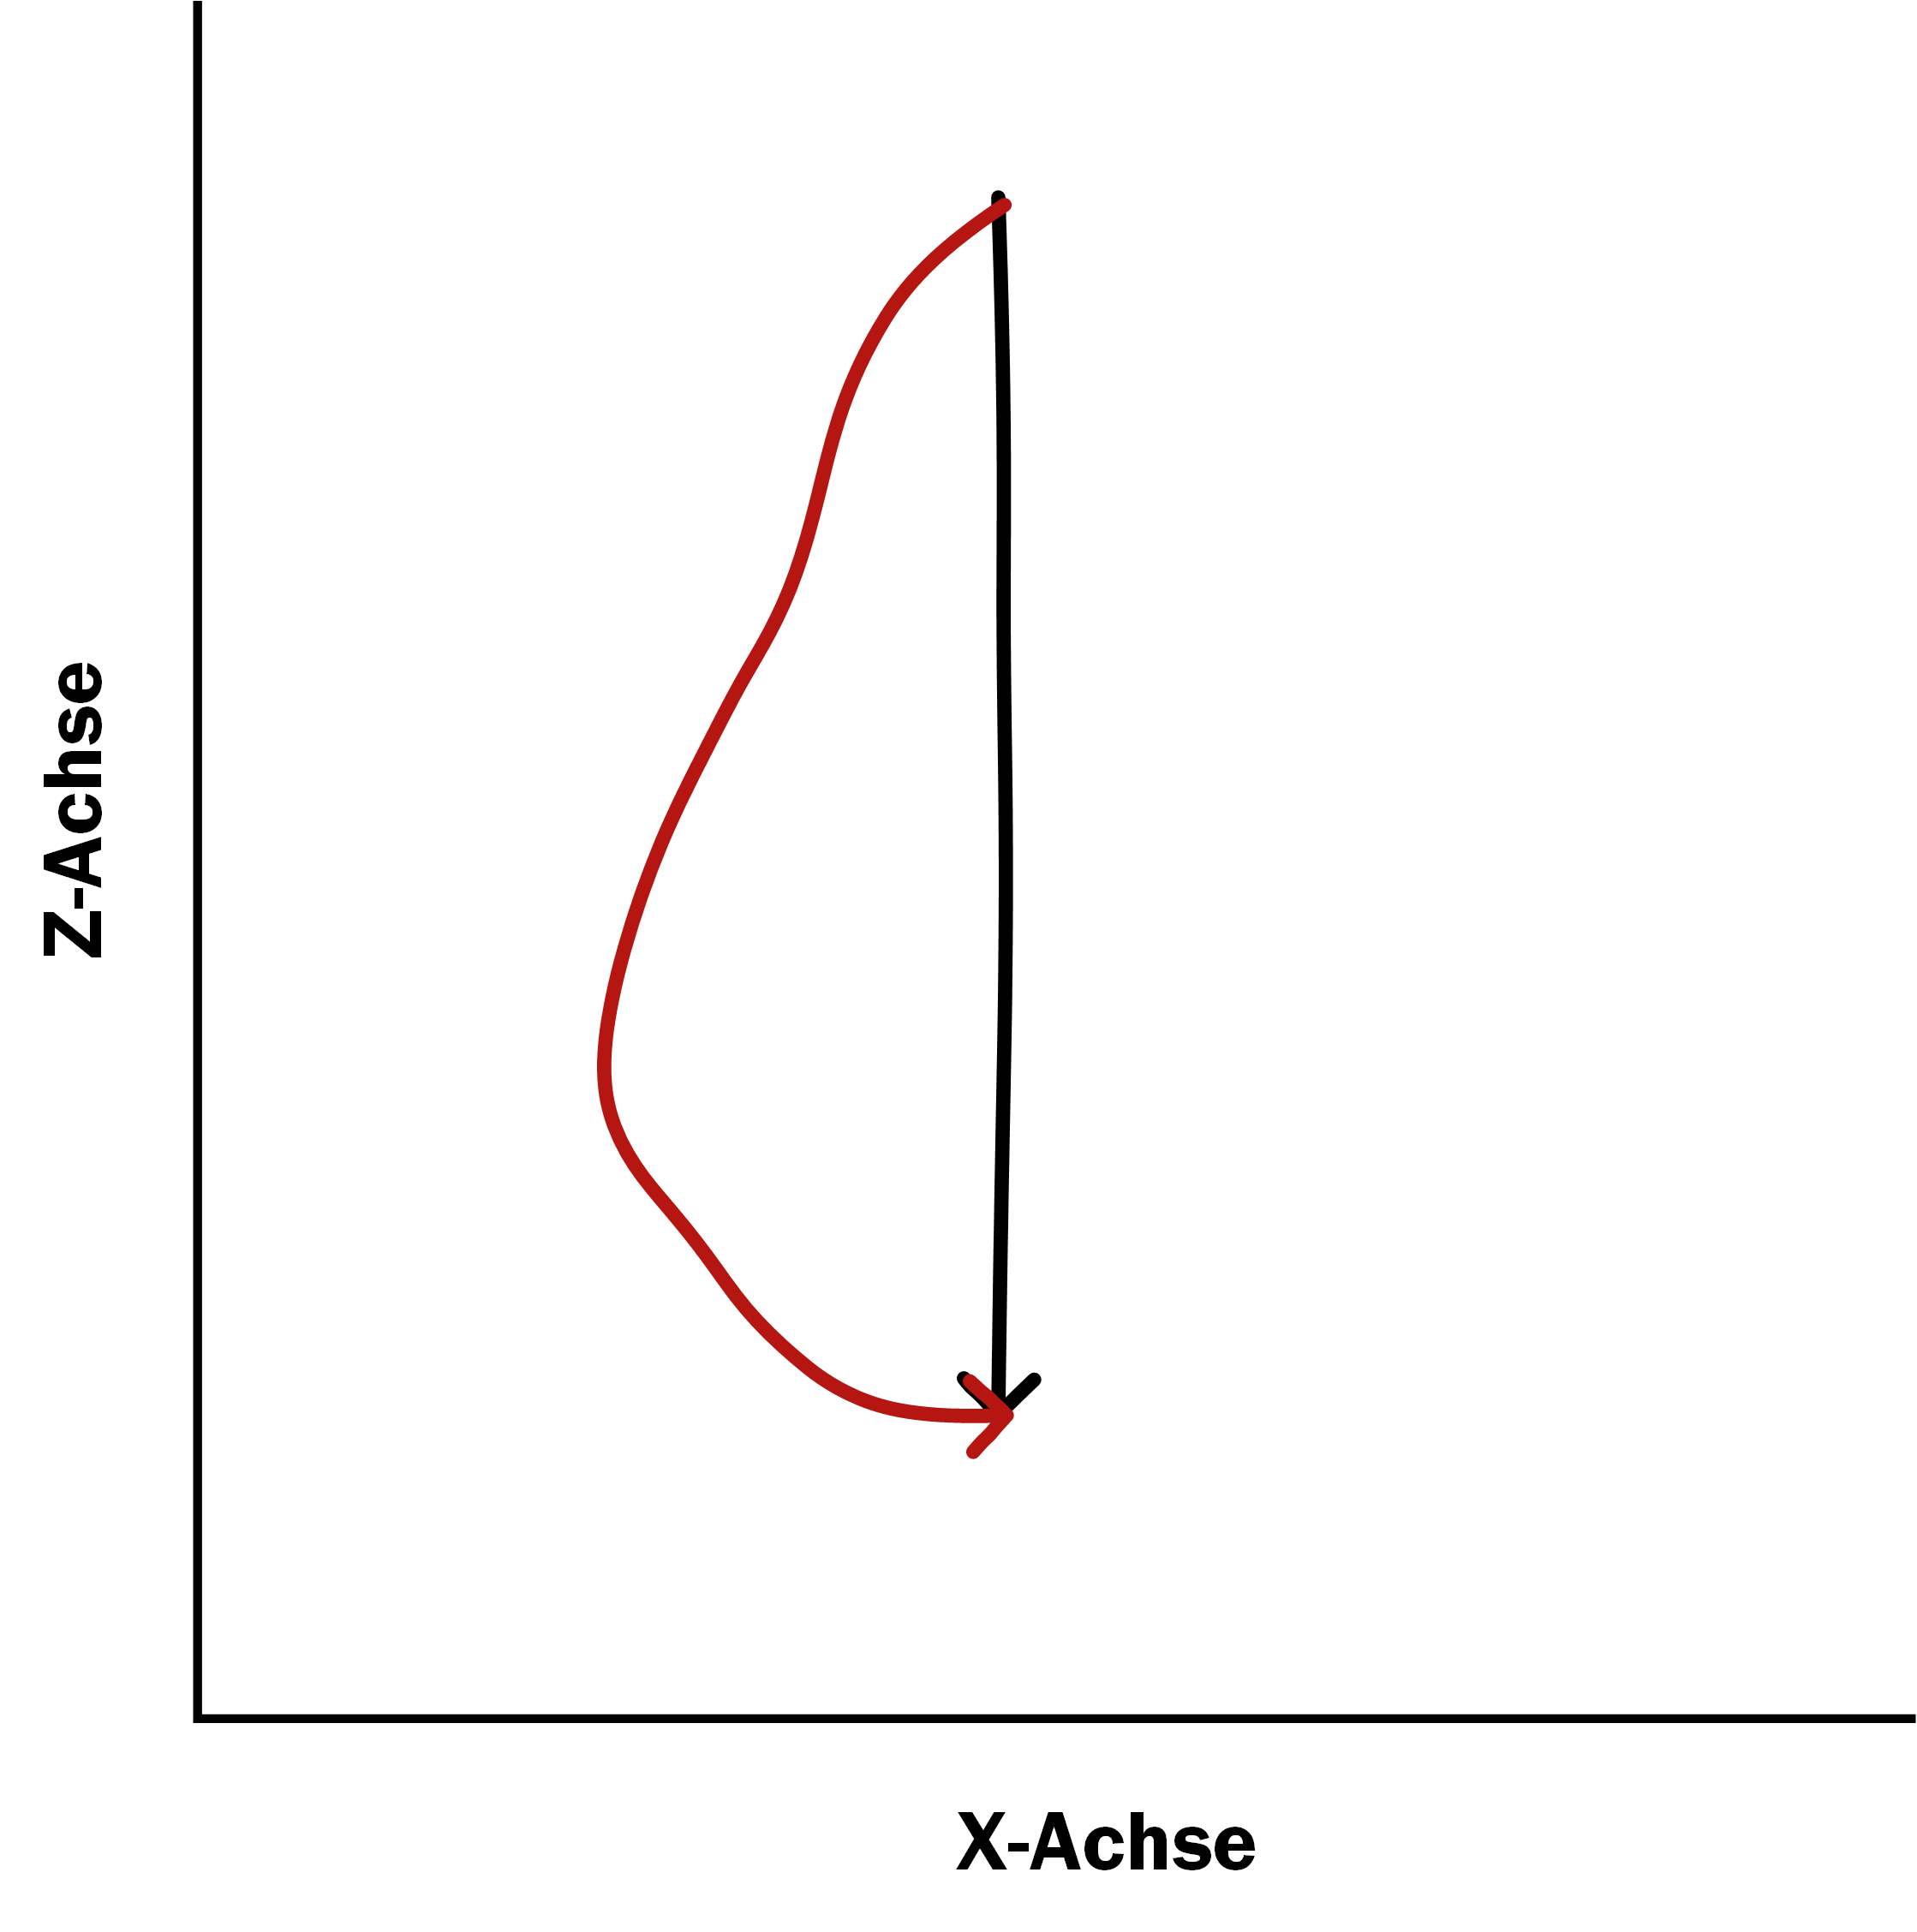
\includegraphics[scale=0.7]{fig/traj1}}
	\hfill
	\subfigure[]{%
		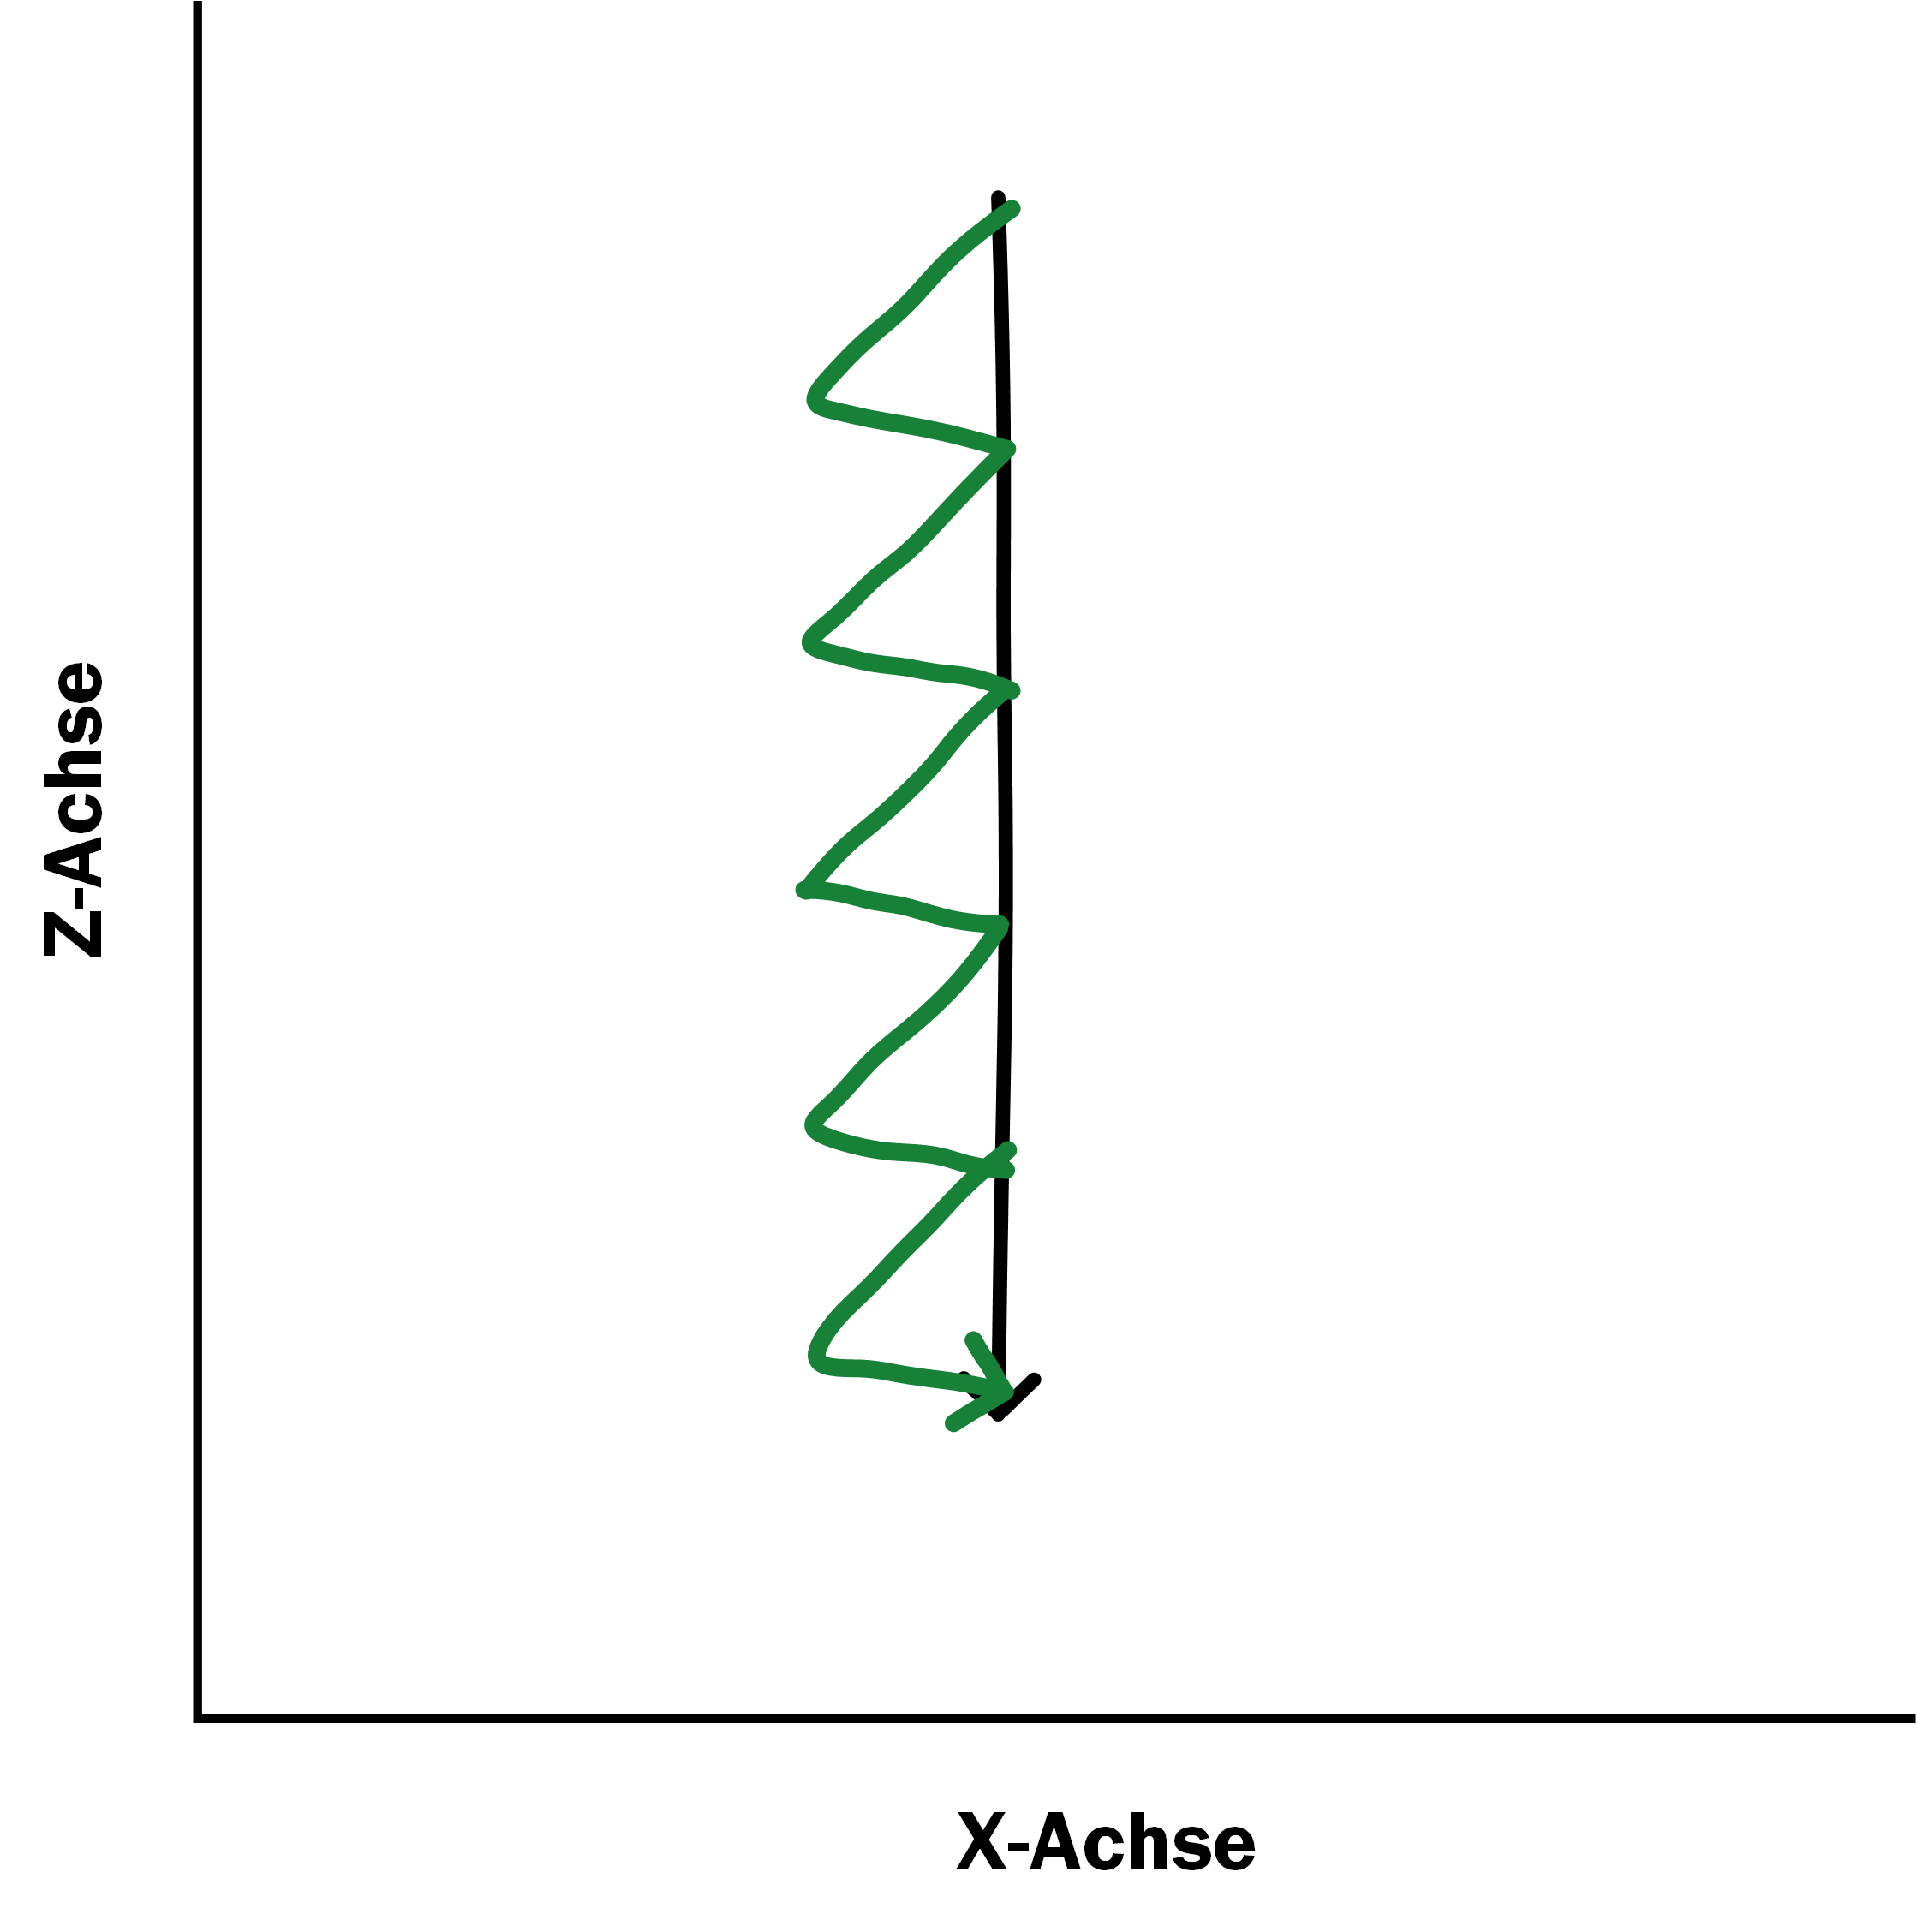
\includegraphics[scale=0.7]{fig/traj2}}
	\caption[Trajektorien des Greifers]{Die dargestellten Graphen stellen die gewünschte Trajektorie (schwarz) und die realen Trajektorien des Greifers dar. Dabei handelt es sich um eine lineare Absenkung auf der Z-Achse. Links: Trajektorie (rot) bei Angabe der Zielpose. Rechts: Trajektorie (grün) bei Angabe von Zwischenposen auf der gewünschten Trajektorie. Bildquelle: \cite{muggler2013torque}}	
	\label{fig:traj}
\end{figure}

\subsubsection{Aktionen der Roboter}

In diesem Unterkapitel wird sehr kurz auf die Aktionen eingegangen, die für die Roboter implementiert wurden. Aus Gründen des Umfangs wird dabei auf Grafiken, wie zum Beispiel UML-Diagramme, verzichtet. Aktionen die nur für einen Roboter implementiert wurden, sind speziell gekennzeichnet.

\paragraph{Greifer öffnen und schließen} Diese Aktion sind eigentlich zwei. Für beide Roboter wurde eine Aktion für das Öffnen und eine für das Schließen implementiert. Beim Öffnen fahren die beiden Finger des Greifers auf ihre maximal Position. Beim Schließen fahren die beiden Finger auf die Nullstellung. Befindet sich ein Objekt im Greifer versuchen die Finger den Schluss. Da die Kraft des Greifers jedoch nicht reicht und die Finger nur auf Spindeln sitzen, befinden sich die Finger am Ende der Aktion nicht in der Nullstellung.

\paragraph{Greifer in Pose bringen} Bei dieser Aktion wird als Parameter die sechsdimensionale Pose benötigt. Diese kann sich im globalen, als auch im lokalen Koordinatensystem des Roboters befinden und muss als solche mit einem Flag gekennzeichnet sein. Bei der Aktion wird zunächst die Gelenkeinstellung durch die inverse Kinematik ermittelt und anschließend mit der Methodik aus Kapitel \ref{sec:impl-res-ak} angesteuert. Zwei Sonderfälle dieser Aktion wurden für die Bewegung in die \textit{Candle}- oder \textit{Fold}-Pose implementiert.

\paragraph{Greifer an eine Pose annähern} Mit der Annäherung ist in diesem Fall eine lineare Trajektorie entlang der Z-Achse des Greifers in der Endpose gemeint. Auch hier wird als Parameter die Zielpose im lokalen oder globalen Koordinatensystem benötigt. Aus dieser Pose wird ein Vektor bestimmt. Dieser läuft entlang der Z-Achse der Greifers und hat eine Länge von vier Zentimetern. Entsprechend der Entwicklung aus Kapitel \ref{sec:impl-res-lb} werden acht Posen im fünf Millimeter Abstand auf diesem Vektor bestimmt und nacheinander angefahren.

\paragraph{Objekt aufheben} Diese Aktion ist eine Task, bei der seriell Aktionen ausgeführt werden. Als Parameter wird die Position des Zielobjektes benötigt, diese kann als lokaler Kontext angegeben werden oder mit einem Zeiger auf das Objekt im globalen Kontext. Neben der Position des Objektes wird die Rotation um die Z-Achse des Objektes berücksichtigt, da die X-Achse des Greifers parallel zur X-Achse des Objektes liegen muss. Bei der Durchführung wird zunächst der Greifer in einem vier Zentimeter Abstand in Position gebracht. Anschließend wird Greifer geöffnet und an die Position des Objektes angenähert. Folgend wird der Greifer geschlossen und der Arm in die \textit{Candle}-Pose gebracht. Für Rose gibt es eine erweiterte Form dieser Aktion, dabei wird Kontakt zur Naherkennung aufgenommen, um das Objekt visuell zu lokalisieren. Diese Koordinierung wird genutzt, um den Arbeitsraum des Roboters an die Position des Objektes anzupassen.

\paragraph{Objekt ablegen} Ähnlich dem Aufheben ist auch diese Aktion eine Task. Im Gegensatz dazu werden die Aktionen in einer anderen Reihenfolge ausgeführt. So fährt der Greifer zunächst in eine Pose etwas über dem Ziel. Öffnet anschließend die Finger um sich abschließend von dem Objekt zu entfernen. Dies geschieht auf einer linearen Trajektorie um das Objekt nicht zu verschieben. Abschließend bewegt der Arm sich in die \textit{Candle}-Pose.

\paragraph{Position einnehmen}
Diese Aktion betrifft nur Rose. Dabei fährt die mobile Plattform an eine neue Position. Dafür wird als Parameter eine X- und Y-Koordinate im globalen Koordinatensystem benötigt. Es werden keine rotierenden Bewegungen ausgeführt. Damit bleibt die Ausrichtung der Plattform gleich. Zur Lokalisierung wird dabei eine Mischung aus SLAM und Odometriedaten genutzt (siehe \ref{sec:impl-lopo}).

\paragraph{Übergabe} Die Übergabe ist die zentrale Aktion dieser Arbeit. Der Ablauf dieser ist bereits in Kapitel \ref{fun:han} und in den Abbildungen \ref{fig:gripper1}, \ref{fig:gripper2} und \ref{fig:gripper3} erläutert. Die Koordinierung dieser Aufgabe wird durch den RATSCore abgebildet. Die Positionsbestimmung kann durch eine direkte Koordinierung zwischen den Robotern stattfinden.

\subsection{Raumüberwachung - RATSHawk}
Die Raumüberwachung übernimmt die Detektion und Lokalisierung von Objekten im Raum. Dazu dient eine XTion-Kamera die an der Wand angebracht ist. Für das MRS wurde dafür ein eigener RATSMember, der RATSHawk, geschaffen. Momentan besitzt dieser Agent nur eine einzige Aktion: ein Objekt anhand seiner Farbe im Raum zu detektieren und die Position im globalen Kontext zu bestimmen. Als Parameter wird dafür ein Zeiger auf das gesuchte Objekt im globalen Kontext benötigt. Die Informationen über die Farbwerte des Objektes im HSV-Farbraum müssen im globalen Kontext unter dem Objekt abgelegt sein. Nach Ausführung der Aktion wird im Erfolgsfall die Position des Objektes in den globalen Kontext eingetragen. Die folgenden Kapitel befassen sich mit der verwendeten API \textit{Point Cloud Library} und den Subsequenzen zur Detektion und Lokalisierung des Objektes.

\subsubsection{PCL \& ROS}
Für die Anbindung der Kamerasysteme an ROS existieren die Pakete OpenNI2 und OpenNI2Launch. Diese generieren aus den Bildern der XTions Punktwolken, die mit Hilfe von Topics empfangen werden können. Für die Weiterverarbeitung der Punktwolken wird in dieser Arbeit die Point Cloud Library (PCL) genutzt. Diese bietet unter anderem verschiedene Filter, Feature und Keypoint Detektion, sowie Segmentierungen und Erkennungen. Einziges Problem ist Konvertierung der einzelnen Punktwolken-Formate. Jedoch stellt die PCL-API Methoden zur Umwandlung bereit. Dabei muss jedoch die Art der Punktwolke, zum Beispiel chlorierte Punktwolke (XYZRGB) oder Intensität-Punktwolke (XYZI), berücksichtigt werden. Für die XTion Kamerasysteme können entweder XYZ-Punktwolken ohne Farbwerte oder XYZRGB-Punktwolken mit Farbwerten im RGB-Farbraum genutzt werden.

\subsubsection{Detektion}
Die Detektion in dieser Arbeit basiert auf den Farb- und Geometriemerkmalen des Objektes. Dazu sind mehrere Schritte nötig. Nach der Konvertierung der Punktwolke $P$ wird zunächst die Anzahl der Punkte $p_i$ reduziert, indem alle Punkte die zum Boden $P_B$ gehören aus der Punktwolke entfernt werden. Die dazu gehörigen Punkte werden mit Hilfe des RANSAC-Algorithmus ausgewählt. Dafür wird ein planares Modell angenommen. Damit nicht auch Punkte des auf dem Boden liegenden Objektes entfernt werden, wird der Schwellwert für die Distanz zwischen Modell und Punkt auf 5 Millimeter gesetzt. Die Anzahl der benötigten Iterationen ist durch die Anzahl der Punkte, die für das Modell benötigt werden, und dem Anteil der Punkte des Bodens gegeben. Diese Funktion wird von der PCL-API zur Verfügung gestellt. Anschließend wird die restliche Punktwolke nach den übergebenen Farbwerten im HSV-Farbraum gefiltert. Dabei werden alle Punkte die außerhalb der Schranken liegen aus der Punktwolke entfernt. Dadurch ergibt sich für die neue Punktwolke $P_{Farb}$:

\begin{equation}
	\forall p_i \in (P - P_B): ((h_{min} \leq p_i^h \leq h_{max}) \wedge (s_{min} \leq p_i^s \leq s_{max}) \wedge (v_{min} \leq p_i^v \leq v_{max})) 
	\implies p_i \in P_{Farb}
\end{equation}

Anschließend wird $P_{Farb}$ in einzelne Punktwolken $P_{Obj}^i \in S_{Seq}$ segmentiert. Dies ist nötig, damit verschiedene Objekte mit der gleichen Farbe, unterschieden werden können. Dafür wird folgender Algorithmus verwendet. Zunächst wird eine leere Menge $S_{Seq}$ definiert. Diese enthält alle Punktwolken-Segmente die durch den Algorithmus gefunden werden. Außerdem wird eine Liste $L$ mit Punkten initialisiert.Für alle Punkte $p_i \in P_{Farb}$ werden folgende Schritte durchgeführt: $p_i$ wird $L$ hinzugefügt. Dabei werden alle Punkte $p^i_j$ die in der Nachbarschaft $P^i$ von $p^i$ liegen gesucht.  Die Nachbarschaftsbeziehung kann durch einen k-d-Baum angegeben werden. Wenn die Distanz zwischen $p^i_j$ und $p^i$ kleiner dem gegebenen Schwellwert $d$ ist, wird der Punkt $p^i_j$ der Liste $L$ hinzugefügt und aus $P_{Farb}$ entfernt. Anschließend wird der Schritt für alle neuen Punkte in $L$ wiederholt. Ist in der letzten Wiederholung kein neuer Punkt hinzugekommen und ist $|L| > N$ wird $L$ als neue Punktwolke $S_{Seq}$ hinzugefügt und anschließend geleert. Dieser Vorgang wird wiederholt bis $|P_{Farb}| = 0$. Anschließend hat man eine Menge $S_{Seq}$ an Punktwolken, deren Punkte nah beieinander liegen und eine entsprechende Größe $N$ haben:

\begin{equation}
\forall P_i \in S_{Seq}: |P_i| > N 
\end{equation}

Um nun ein Segment dem Objekt zuzuweisen wird die Anzahl der Punkte eines Segments mit der hinterlegten Anzahl an Punkten für das Objekt verglichen. Da die Anzahl der Punkte von der Entfernung zur Kamera und Lage des Objektes abhängig ist, gilt dieses nur als grobes Kriterium. Bei der Berechnung zur Lokalisierung werden deshalb noch weitere geometrischen Merkmale überprüft.

\subsubsection{Lokalisierung}
Nachdem die Punktwolke für das Objekt extrahiert wurde, wird nun die Position und Rotation des Objektes bestimmt. Dafür wird zunächst eine Oriented Bounding Box (OBB) für das Objekt bestimmt. Eine Oriented Bounding Box entspricht einer Axis Aligned Bounding Box (AABB) die an den Eigenvektoren der Punktwolken orientiert ist. Eine Bounding Box entspricht einem Quader, in dem alle Punkte der Punktwolke enthalten sind. Die AABB ist an den Achsen des Koordinatensystem ausgerichtet. Für die Bestimmung der einzelnen Merkmale existiert in der PCL-API bereits ein vorgefertigter Algorithmus. Mit Hilfe diesem lässt sich neben dem minimalen und maximalen Punkt der Punktwolke auch der Mittelpunkt und die Rotationsmatrix für die OOB bestimmen. An Hand der Daten der OOB wird nun nochmal ein Abgleich der Geometrischen Eigenschaften des Objektes gemacht, dabei wird das Seitenverhältnis mit den hinterlegten Daten verglichen. Stimmen diese überein, wird aus der Kamerapose im globalen Koordinatensystem und der Objektpose im Kamera-Koordinatensystem die Objektpose im globalen Koordinatensystem berechnet. Jedoch zeigte ein Vergleich zwischen der realen und der berechneten Position Differenzen. Eigene Tests zeigten, dass die Differenzen Positionen bezogen sind. Die Ursache davon liegt vermutlich bei einer Verzerrung der Kameralinse oder einem fehlerhaften Parameter beim Registrierung der RGB-Bilder auf das IR-Bild. Um diese Verzerrung zu korrigieren wird nun ein Ausgleich-Modell verwendet, dass auf den gemessenen Testdaten beruht. Dazu wird zunächst auf dem Mittelpunkt des Kamerabildes der Normalenvektor der Kameraebene gesetzt und der Schnittpunkt mit der planaren Ebene des Bodens bestimmt. Anschließend wird die Distanz in der X- und Y- Richtung der Bildebene zum Objekt bestimmt und je nach Richtung mit einem Korrekturfaktor multipliziert. Diese Korrektur erbringt eine Genauigkeitssteigerung, sodass die Positionsbestimmung eine Genauigkeit von fünf Zentimetern erreicht. 

\subsection{Nahfelderkennung - RATSEye}
Im Gegensatz zur Raumüberwachung sitzt die Kamera nicht an der Wand, sondern am Roboter direkt. Dies betrifft in diesem Fall Rose. Die Nahfelderkennung ist als selbstständiger RATSMember, dem RATSEye, umgesetzt. Genau wie der RATSHawk besitzt das RATSEye nur eine Aktion zur farbbasierten Detektion und Lokalisierung. Aufgrund des geringen Abstandes zum Objekt hat dieser Agent gegenüber dem RATSHawk Vor- aber auch Nachteile. Auf der einen Hand ist die Genauigkeit der Ergebnisse auf dieser Distanz viel höher. Auch notwendige Korrekturen, wie beim RATSHawk, sind nicht nötig. Auf der anderen Hand benötigt der Agent die Vorarbeit eines anderen Agenten um arbeiten zu können. Da die Kamera am Arm von Rose angebracht ist, muss dieser erst in die \textit{Candle}-Pose gebracht werden. dies erhöht den Koordinierungsaufwand. Ein weitere Nachteil ist die schlechte Hardware, die dem Agenten zur Verfügung steht. Dadurch, dass die Kamera an den eingebauten Rechner in der mobilen Plattform gebunden ist, dauern Auswertungen der Punktwolken länger. Außerdem ist durch die Belastung des Systems eine Verzögerung der Punktwolken gegeben. Da die Berechnung für das Hardwaresystem belastend sind wird von einer wiederholenden Ausführung abgesehen und die Aktion nur bei Bedarf ausgeführt. Dies und die Verzögerung kann dazu führen, dass die Daten nicht dem aktuellen Ausschnitt entspricht, an dem sich der Agent befindet. Um dies zu umgehen wurde ein paralleler Thread aufgebaut. Dieser empfängt die Punktwolken und legt die aktuellste in einem Speicher ab. Wird nun die Hauptfunktion ausgeführt blockiert diese ihren eigenen Thread mit einem Mutex. Der Datenthread hebt diese Sperre auf, sobald eine neues Punktwolke im Speicher liegt. Daraufhin blockiert der Hauptthread den Datenthread mit einem weiteren Mutex. Dies ist nötig, da während der Analyse neue Punktwolken eintreffen könnten und den Speicher überschreiben würden. Nach der Detektion und Lokalisierung wird diese Sperre wieder aufgehoben. Die Detektion und Lokalisierung laufen genauso ab, wie bei der Raumüberwachung. Nur die Korrektur der Lokalisierung ist nicht nötig.

Während der Testphase kam es bei der Nahfelderkennung zu zunächst unerklärlichen temporären Problemen. Dabei konnte das Objekt nicht detektiert werden. Dies lies sich auf zu kleine Punktwolken zurückführen. Eine Inspektion der aufgenommenen Bilder ergab, dass einzelne Bilder sehr dunkel waren. Bei einer genaueren Untersuchen stellte sich heraus, dass Reflexionen der Beleuchtung durch die spiegelnde Oberfläche der mobilen Plattform direkt in die Kamera blendeten. Diese führte einen automatischen Helligkeitsausgleich durch und verdunkelte das komplette Bild. Diese Problem konnte mechanisch umgangen werden, indem die spiegelnde Fläche mit schwarzem Klebeband verdeckt wurde.

\subsection{Koordinierung}
Die Koordinierung innerhalb dieses MRS ist über zwei Methoden möglich: die zentrale Koordinierung über den RATSCore oder die direkte Kommunikation zwischen zwei Agenten. Beide Varianten nutzen die gleiche Schnittstelle beim Empfänger, dadurch bleibt das System flexibel und erweiterbar. Diese Schnittstelle ist mit der ROS Action-Lib realisiert, wie in TODO beschrieben. Im Folgenden soll an Beispielen erklärt werden, wie die Koordinierung beim RATSCore und beim RATSMember implementiert wurden.

\subsubsection{Koordinierung beim RATSCore}
\subsubsection{Koordinierung beim RATSMember}
\subsection{Lokale Positionierung}
\label{sec:impl-lopo}
\subsection{Handoverpoint}
\label{sec:impl-hop}
\clearpage
%%%%%%%%%%%%%%%%%%%%%%%%%%%%%%%%%%%%%%%%%%%%%%%%%%%%%%%%%%%%%%%%%%%%%%%
%% Zusammenfassung und Ausblick
\section{Test und Bewertung}
\label{sec:test}
Dieses Kapitel umfasst Testreihen zur Bewertung des MRS. Diese Testreihen folgen dem \textit{Top-Down} Prinzip und sind nicht als vollwertige Softwaretests zu sehen, da unter anderem auch das Zusammenspiel der Konzepte und der Hardware getestet wird. Zunächst wird das Gesamtsystem getestet, da die einzelnen Algorithmen und Konzepte zum Teil schon in ihrer Entwicklungsphase getestet wurden. Kommt es zu Fehlschlägen des Gesamtsystems, wird der Fehlschlag analysiert und die betreffenden Subsysteme getestet. Diese Tests sind vor allem als funktionsorientierter Test zusehen. Es werden also keine Daten- oder Kontrollflüsse getestet, sondern der Fokus auf Positiv- und Negativtests gelegt. Auch die Ursache-Wirkung-Analyse ist für die Subsysteme angewendet. 

Die Tests für das Gesamtsystem werden mit Hilfe von funktionalen Äquivalenzklassen durchgeführt. Dazu wurde folgendes Szenario 24 mal ausgeführt: Das Zielobjekt liegt an einer Position im Raum. Rose befindet sich in einer definierten Startposition. Das System bekommt die Aufgabe das Objekt aufzuheben und an einer definierten Stelle auf dem Tisch abzulegen. Die Position des Objektes im Raum variiert bei den Testfällen und ist in Äquivalenzklassen unterteilt. Diese sind an den notwendigen Bewegungen der Plattform orientiert. Die Äquivalenzklassen setzen sich aus der Achse und der Strecke der Bewegung zusammen: \textit{ X-Kurz}, \textit{ X-Lang}, \textit{ X-Kurz, Y-Kurz}, \textit{ X-Lang, Y-Kurz}, \textit{ X-Kurz, Y-Lang}, \textit{ X-Lang, Y-Lang}. Wird eine Achse nicht erwähnt findet keine Bewegung entlang dieser statt. Kurz steht für eine Bewegungsdistanz kleiner 50 Zentimeter entlang der angegeben Achse. Die Tabelle \ref{tab:messw} bildet alle Testfälle mit allen Messergebnissen, die während dieses Szenarios erzielt wurden, ab. Dazu zählen die Genauigkeit der Raumüberwachung $\gamma$ und der Differenz zwischen Odometriedaten und Laserdaten $\eta$ in Zentimetern, die Anzahl der Korrekturversuche $k$ der mobilen Plattform, die Anzahl der Verhandlungsversuche $j$ für den Übergabepunkt und die Genauigkeit bei der Übergabe $\iota$ in Zentimetern. Die letzte Spalte bildet den Erfolg des Testfalls oder den auftretenden Fehler ab. Dabei traten drei Fehlerwirkungen auf: \textit{Fehler 1} steht für einen Abbruch bei der Aufnahme des Objektes, zum Beispiel durch eine Überschreitung der Versuchsschranke, zehn Versuche, oder einem Fehlgriff. \textit{Fehler 2} bildet den Abbruch während der Bestimmung der Übergabeposition ab. Dies kann nur durch ein überschreiten der Verhandlungsschranke, maximal zehn Verhandlungen, ausgelöst werden. \textit{Fehler 3} tritt bei einer falschen Übergabe auf. Die Ursache der Fehler wird im folgenden analysiert. 

\begin{center}
	\begin{longtable}{|c|c|c|c|c|c|c|c|}
		\hline
		Testlauf & Äquivalenzklasse &$\gamma$ & $\eta$ & $k$ & $j$ & $\iota$ & Erfolg oder Fehler\\
		\hline
		\hline
		1 & X-Kurz & $\left(\begin{array}{c} 2,2 \\ 1,6\end{array}\right)$ & $\left(\begin{array}{c} 3,2 \\ -0,4\end{array}\right)$ & $0$ & $2$ & <1cm& \checkmark\\
		\hline
		2 & X-Kurz &  $\left(\begin{array}{c} -2,1 \\ 1,3\end{array}\right)$ & $\left(\begin{array}{c} 4,1 \\ -0,3\end{array}\right)$ & 0 & 4 & <1cm & \checkmark\\
		\hline
		3 & X-Kurz &  $\left(\begin{array}{c} 1,4 \\ 2,2\end{array}\right)$ & $\left(\begin{array}{c} 3,5 \\ -0,5\end{array}\right)$ & 0 & 2& <1cm& \checkmark\\
		\hline
		4 & X-Kurz &  $\left(\begin{array}{c} 2,3 \\ -2,1\end{array}\right)$ & $\left(\begin{array}{c} 3,7 \\ -0,3\end{array}\right)$ & 0& 2&<1cm & \checkmark\\
		\hline
		5 & X-Lang &  $\left(\begin{array}{c} -1,6 \\ 1,8\end{array}\right)$ & $\left(\begin{array}{c} 5,2 \\ -0,7\end{array}\right)$ & 1& 2& <1cm& \checkmark\\
		\hline
		6 & X-Lang &  $\left(\begin{array}{c} 1,4 \\ 1,4\end{array}\right)$ & $\left(\begin{array}{c} 6,1 \\ -0,8\end{array}\right)$ & 1& 3& <1cm& \checkmark\\
		\hline
		7 & X-Lang &  $\left(\begin{array}{c} 1,3 \\ -2,2\end{array}\right)$ & $\left(\begin{array}{c} 7,2 \\ -0,8\end{array}\right)$ & 0& 2& <1cm& \checkmark\\
		\hline
		8 & X-Lang &  $\left(\begin{array}{c} 5,4 \\ 1,3\end{array}\right)$ & $\left(\begin{array}{c} 6,8 \\ -0,5\end{array}\right)$ & 1& 2& <1cm& \checkmark\\
		\hline
		9 & X-Kurz, Y-Kurz &  $\left(\begin{array}{c} 2,1 \\ -1,5\end{array}\right)$ & $\left(\begin{array}{c} 10.4 \\ -4,8\end{array}\right)$ & >10& -& -& Fehler 1\\
		\hline
		10 & X-Kurz, Y-Kurz &  $\left(\begin{array}{c} 1,2 \\ 3,8\end{array}\right)$ & $\left(\begin{array}{c} 4,2 \\ -7,4\end{array}\right)$ & 1& 3& <1cm& \checkmark\\
		\hline
		11 & X-Kurz, Y-Kurz &  $\left(\begin{array}{c} -2,4 \\ 4,2\end{array}\right)$ & $\left(\begin{array}{c} 3,7 \\ -6,3\end{array}\right)$ & 2& 4& <1cm& \checkmark\\
		\hline
		12 & X-Kurz, Y-Kurz &  $\left(\begin{array}{c} -3,2 \\ -2,1\end{array}\right)$ & $\left(\begin{array}{c} 6,1 \\ -4,2\end{array}\right)$ & 1& 2& 3,2& Fehler 3\\
		\hline
		13 & X-Lang, Y-Kurz &  $\left(\begin{array}{c} -4,1 \\ -2,8\end{array}\right)$ & $\left(\begin{array}{c} 3,8 \\ -7,2\end{array}\right)$ & 1& 3& 4,2& Fehler 3\\
		\hline
		14 & X-Lang, Y-Kurz &  $\left(\begin{array}{c} 7,2 \\ 1,2\end{array}\right)$ & $\left(\begin{array}{c} 9,4 \\ -4,8\end{array}\right)$ & 2& 4& 4,5& Fehler 3\\
		\hline
		15 & X-Lang, Y-Kurz &  $\left(\begin{array}{c} -1,4 \\ 8,1\end{array}\right)$ & $\left(\begin{array}{c} 6,2 \\ -5,5\end{array}\right)$ & 2& 3& <1cm& \checkmark\\
		\hline
		16 & X-Lang, Y-Kurz &  $\left(\begin{array}{c} 2,4 \\ 1,3\end{array}\right)$ & $\left(\begin{array}{c} -1,2 \\ -4,2\end{array}\right)$ & 2& 3& <1cm& \checkmark\\
		\hline
		17 & X-Kurz, Y-Lang &  $\left(\begin{array}{c} 1,2 \\ -3,4\end{array}\right)$ & $\left(\begin{array}{c} 5,4 \\ -22,8\end{array}\right)$ & >10& -&- & Fehler 1\\
		\hline
		18 & X-Kurz, Y-Lang &  $\left(\begin{array}{c} 3,8 \\ 2,1\end{array}\right)$ & $\left(\begin{array}{c} 3,2 \\ -17,2\end{array}\right)$ & 2& >10& -& Fehler 2\\
		\hline
		19 & X-Kurz, Y-Lang &  $\left(\begin{array}{c} 2,5 \\ 2,4\end{array}\right)$ & $\left(\begin{array}{c} 1,6 \\ -20,1\end{array}\right)$ & 1& 7& <1cm& \checkmark\\
		\hline
		20 & X-Kurz, Y-Lang &  $\left(\begin{array}{c} 1,6 \\ 2,7\end{array}\right)$ & $\left(\begin{array}{c} 4,2 \\ -19,8\end{array}\right)$ & 2& 8& 4,2cm& Fehler 3\\
		\hline
		21 & X-Lang, Y-Lang &  $\left(\begin{array}{c} 3,2 \\ -1,7\end{array}\right)$ & $\left(\begin{array}{c} 3,8 \\ -21,2\end{array}\right)$ & 1& 6& 5,6cm& Fehler 3\\
		\hline
		22 & X-Lang, Y-Lang &  $\left(\begin{array}{c} 2,4 \\ 2,1\end{array}\right)$ & $\left(\begin{array}{c} 2,8 \\ -18,4\end{array}\right)$ & 2& 5& <1cm& \checkmark\\
		\hline
		23 & X-Lang, Y-Lang &  $\left(\begin{array}{c} -3,3 \\ 1,6\end{array}\right)$ & $\left(\begin{array}{c} 2,8 \\ -31,4\end{array}\right)$ & >10& -& -& Fehler 1\\
		\hline
		24 & X-Lang, Y-Lang &  $\left(\begin{array}{c} 2,7 \\ 1,8\end{array}\right)$ & $\left(\begin{array}{c} 3,1 \\ -16,1\end{array}\right)$ & 2& 8& 6,2& Fehler 3\\
		\hline
	\caption{Messwerte der Testphase}
	\label{tab:messw}
	\end{longtable}
\end{center}

Zusammengefasst ergibt sich, dass das Robotersystem eine Erfolgsquote von ca. 60 Prozent hat. Dabei ist auffällig, dass die Fehler sich bei einer großen Distanz auf der Y-Achse häufen. Um die Fehlerquelle genauer identifizieren zu können werden zunächst die einzelnen Aktionen aufgelistet. Anschließend wird eine Vorauswahl getroffen, welche Aktionen für den Fehler verantwortlich sein können. Anschließend werden diese Aktionen genauer untersucht. Fehler 1 gehen fünf Aktionen voraus: Objekt identifizieren und lokalisieren, Rose an die Zielposition bewegen, Naherkennung des Objektes, Korrekturbewegung und Objekt aufheben. Diese können alle potenzielle Fehlerquellen sein. Jedoch lassen sich einzelne Aktionen durch Subsystemtests schon ausschließen. So ist die Raumüberwachung mit einer Genauigkeit von fünf Zentimetern entwickelt worden. Die Werte aus der Tabelle ergeben, dass diese Genauigkeit auch eingehalten wurden. Ausnahmen bilden die Testläufe 14 und 15. Zwischen Fehler 1 und 2 liegt nur die Bestimmung der Übergabeposition, sowie die Korrektur der Position von Rose. Dies betrifft also die Lokalisierung und Positionierung der mobilen Plattform, sowie das Konzept der Bestimmung der Korrektur. Zu Fehler 3 führen die Positionierung und die inverse Kinematik. Im Folgenden werden diese einzelnen Aktionen getestet und mögliche Folgefehler analysiert.

\subsection{Genauigkeit Inverse Kinematik}
\label{sec:iktest}
Für die Tests der inversen Kinematik wurden 25 Posen im lokalen Koordinatensystem von Dummy definiert. Diese wurden nacheinander vom Greifer von Dummy angefahren. Zwischen den einzelnen Posen wurde die \textit{Candle}-Pose eingenommen. Bei allen Posen wurde die Distanz zwischen Greiferpose und Zielpose aufgenommen. Die Greiferposen wurden mit der RViz-Anwendung von ROS gemessen. Diese gibt Position und Rotation des Greifers aus. Anschließend wurden die Differenzen der einzelnen Posen berechnet und der arithmetische Mittel-, der Min- und der Max-Wert festgestellt und in eine CSV-Datei abgelegt. Die Ergebnisse sind Anhang \ref{app:tdik} zu entnehmen. Entscheidend sind die maximalen Abweichungen, diese betragen linear 3,78 Millimeter und 0,66 \textdegree für den rotierenden Anteil. Diese Ergebnisse der inversen Kinematik sind für diese Arbeit sehr gut und erfüllen die selbst gesetzten Anforderungen. Folglich ist die inverse Kinematik nicht die Ursache für die obigen Fehler.

Ein weiterer Bestandteil ist der Bewegungsplaner für die linearen Trajektorien. Bei diesem werden Zwischenpose berechnet. Da diese jedoch durch Matrixmultiplikationen berechnet werden, ist die Wahrscheinlichkeit für einen Fehler so gering, dass die genutzte KDL-Api nicht zusätzlich getestet wurde.
 
\subsection{Test Übergabeposition}
Die Übergabeposition hat zwei mögliche Fehlerquellen: das Konzept der Verhandlung oder der Korrekturbewegung. Auffällig ist Testlauf 18, der als einziger in der Übergabephase abgebrochen hat. Bei diesem konnte man beobachten, dass die mobile Plattform die Korrekturbewegungen nur auf ihrer lokalen X-Achse durchführte. Dabei war die Distanz zwischen den Robotern so gering, dass die Posen der Greifer nicht zu einander passten. Dies führte zu wiederholenden Verhandlungsabbrüchen. Die anschließende Korrektur führte dabei auf die Position vor der letzten Korrektur zurück. Dieses Pendeln zwischen den beiden Position wurde schon in Kapitel \ref{sec:impl-hop} erwähnt und sollte eigentlich durch die Abweichung der Bewegung beseitigt sein. Die Abweichungen auf der lokalen X-Achse der mobilen Plattform ist jedoch zu gering. Dies führte bei Testlauf 18 zum Fehler. Ein Lösungsansatz dafür ist eine bessere Korrekturbewegung, die dynamisch die Korrekturweite bestimmt.

Für die Testläufe mit Fehler 3 ist eine Ungenauigkeit der Position festzustellen. Diese ist auf Schleppfehler durch die Korrekturen zurückzuführen und von der Navigation der mobilen Plattform abhängig.

\subsection{Genauigkeit Navigation}
Die Genauigkeit der Odometrie wurde schon während der Entwicklung getestet und in Kapitel \ref{seq:lok} analysiert. Dabei wurden starke Abweichungen und Varianzen bei Bewegungen entlang der Y-Achse der mobilen Plattform festgestellt. Deshalb wurde die Kopplung an die Sensordaten entwickelt. Wie Tabelle \ref{tab:messw} zeigt sind die Abweichungen zwischen Odometrie $o$ und Laserdaten $l$ gerade bei den genannten Bewegungen sehr hoch. Wobei die $o$ entlang der Y-Achse immer kleiner und entlang der X-Achse größer als $l$ sind. Neben $l$ und $o$ wurde bei den fehlgeschlagenen Testläufen auch die Differenz zur realen Position $p$ im globalen Koordinatensystem genommen. Auffällig dabei ist Testlauf 9. Dabei ist $||p-o||<||p-l||$. Dies lässt sich mit dem Einwand aus Kapitel \ref{sec:impl-lopo} erklären, dass die Auswertung der Laserdaten die Fensterreihe und nicht die Wand detektiert hat. Ansonsten gilt $||p-o||>||p-l||$.  Aber auch die Lokalisierung mit Hilfe der Laserdaten hat Abweichungen von mehreren Zentimetern. Diese addiert mit der geringen Ungenauigkeit der Kamera führt dazu, dass Objekte komplett verfehlt werden. Auch die nötigen Korrekturen erzeugen auf Grund der schlechten Odometriedaten Schleppfehler.

\subsection{Robustheit}
Dieser Test fällt im Vergleich zu den anderen Tests aus der Reihe. Hierbei geht es um das Verhalten im Fehlerfall. Dies soll das RATS-Konzept auf die Nicht-Funktionalen Anforderung der Zuverlässigkeit prüfen. Dazu werden Fehler im System provoziert. Dabei werden folgenden Testszenarien durchgeführt:

\begin{enumerate}
	\item beliebigen RATSMember beenden und neu starten
	\item RATSMember während der Koordinierung beenden
	\item RATSCore zurücksetzen
\end{enumerate}

Das gewünschte Ergebnis für alle Testfälle ist ein Abbruch der aktuellen Aktion und der Übergang in einen sicheren Zustand, dies betrifft vor allem die Roboter. Diese stellen ansonsten ein Sicherheitsrisiko dar. Jedes Szenario wird zehnmal getestet, wobei beim ersten und zweiten die RATSMember variiert werden. Jeder dieser Negativ-Tests endet Positiv. Alle Subsysteme erfüllen die Anforderungen. Dabei bewegen die Roboter ihre Arme nach Inaktivität in die \textit{Fold}-Pose und sind damit in einem mechanisch sicheren Zustand. Beim dritten Szenario beendet der aktuell arbeitende RATSMember zuerst seine Aktion, da keine Kommunikation zwischen RATSMember und RATSCore stattfindet. Im Anschluss folgt der Übergang in den sicheren Zustand.

Im Verlauf dieses Tests kann auch die Wiederherstellbarkeit des Systems getestet werden. Dazu werden nach der Deaktivierung einzelner Knoten diese neu gestartet und die Aktion neu angestoßen. Dabei wird der Aufwand des Neustarts gemessen. Als Kennzahl dient dafür die Anzahl der Eingriffe durch den Anwender. Dabei stellt sich heraus, das ein Neustart des RATSCores am Aufwendigsten ist, da alle RATSMember neu gestartet werden müssen, damit sie sich neu registrieren können. Die Anzahl der Eingriffe bei den anderen Szenarien ist konstant bei zwei. Zum einem muss der RATSMember neu gestartet werden, zum anderen muss die Aktion neu angestoßen werden. Dies bedeutet für das Gesamtsystem eine gute Wiederherstellbarkeit, da der Aufwand gering ist. Nur der RATSCore stellt als Single-Point-of-Failure eine Schwachstelle dar. Eine Alternative dazu wird im Ausblick erwähnt.

\subsection{Zusammenfassung der Tests}
Durch die Ungenauigkeit der Navigation der mobilen Plattform ergeben sich Schleppfehler, die zu großen Ungenauigkeiten führen. Diese sind vor allem bei Bewegungen der lokalen Y-Achse der Plattform merkbar. Auch die eingesetzten Lasersensoren bringen bei diesem Konzept der Steuerung keinen Vorteil. Eine Alternative dazu wird in Kapitel \ref{sec:ausblick} vorgestellt. Die andere Fehlerquelle ist das Korrekturkonzept bei der Übergabe. Bei einer Überarbeitung der Navigation kann die Steigerung der Genauigkeit für ein einfacheres Korrekturkonzept genutzt werden. Dieses beruht auf einer inversen Kinematik, welche die Freiheitsgerade der mobilen Plattform berücksichtigt. Neben den funktionalen Anforderungen wurden auch nicht-funktionale Anforderungen getestet. So wurde die Korrektheit der inversen Kinematik und die Robustheit, sowie Wiederherstellbarkeit des Gesamtsystems untersucht.
\clearpage

%%%%%%%%%%%%%%%%%%%%%%%%%%%%%%%%%%%%%%%%%%%%%%%%%%%%%%%%%%%%%%%%%%%%%%%
%% Zusammenfassung und Ausblick
%%%%%%%%%%%%%%%%%%%%%%%%%%%%%%%%%%%%%%%%%%%%%%%%%%%%%%%%%%%%%%%%%%%%%%%
%% Zusammenfassung und Ausblick
\section{Zusammenfassung und Ausblick}
\label{sec:end}
Dieses Kapitel bildet den Abschluss dieser Arbeit.  Neben einer Zusammenfassung wird ein Ausblick über mögliche Weiterentwicklungen und Verbesserungen gegeben. Dabei wird auf die analysierten Schwachstellen des Systems eingegangen.

\subsection{Zusammenfassung}
In dieser Arbeit wurde ein Multi-Robot-System entwickelt. Dieses nutzt weitere Aktoren und Sensoren, ähnlich einem intelligenten Gebäude, zur Interaktion mit der Umwelt. Zentrale Komponenten dieses Systems sind zwei Roboter. Beide Robotersysteme bestehen aus einem Roboterarm. Der eine Roboter besitzt zudem eine mobilen Plattform, eine 3D-Kamera und einen Lasersensor. Als Anwendungsszenario wurde die Aufnahme durch den mobilen Roboter und die Übergabe an den stationären Roboter implementiert. Dabei wurden 3D-Kameras zur Objekterkennung und -Lokalisierung genutzt. Die Implementierung dafür nutzt Algorithmen aus der Computer Vision, genauer aus der Punktwolken Verarbeitung. Die dabei erreichte Genauigkeit der Sensoren und Algorithmen beträgt fünf Zentimeter bei der Raumüberwachung und fünf Millimeter bei der Nahfelderkennung. 

Zur effizienten Steuerung der Arme wurde iterativ eine eigene inverse Kinematik entwickelt. Diese beruht auf geometrischen Grundsätzen. Bei Tests zeigten diese eine Genauigkeit von circa vier Millimetern von den linearen und 0,6 Grad für den rotierenden Anteil der Zielpose. Für die Bewegung auf einer Trajektorie wurde ein Ansatz gewählt, der mit Hilfe von Wegpunkten den Ausschlag des Greifers verhindert. Nicht genau untersucht wurde die Entwicklung einer genauen Navigation der mobilen Plattform. Aus Gründen der Priorität wurde diese nur sehr rudimentär entwickelt. Bedingt durch ungenaue Odometriedaten bei Bewegungen entlang der Y-Achse kommt es zu hohen Ungenauigkeiten. Auch der Einsatz von Lasersensoren kann diesem nur bedingt entgegenwirken, da diese abhängig von einem Referenzpunkt der Odometrie sind. Andere Ansätze, wie SLAM, sind dabei viel genauer.

 Bei der Entwicklung des MRS wurde auf bestehenden Arbeiten, wie der PEIS-Ökologie, aufgebaut. Neben den Robotern kamen auch weitere eigenständige Sensoren und Aktoren zum Einsatz. RATS erweitert PEIS um die Möglichkeit für parallele und komplexere Koordinierung. Diese kann auch unter den einzelnen Agenten innerhalb eines RATS stattfinden. Da in dieser Arbeit die Anzahl an Robotern, Aktoren und Sensoren sehr gering ist, wurde die Konfiguration des MRS statisch implementiert. Eine Schnittstelle für eine dynamische Konfiguration ist im Konzept für RATS jedoch vorgesehen.

In dieser Arbeit konnte aus Platzgründen nicht auf weitere erarbeitete Konzepte eingegangen werden. Die Grundlagen für diese beruhen auf dieser Arbeit. Auch die Implementierung wurde im Rahmen dieser Arbeit durchgeführt. Dazu gehören Problematiken um den Greifer, der in dieser schriftlichen Ausarbeitung nur am Rande betrachtet wurde. Auf Grund mangelnder Griffigkeit des Greifer zum starren Testobjekt, kam es zum Einsatz des pinken Radiergummis. Dieses weißt einen hohen Reibungskoeffizienten und eine weiche, sowie flexible Struktur auf. Außerdem war es anhand der Farbe leicht zu identifizieren. Ein weiterer Randaspekt ist die Einbindung eines weiteren Aktors in das RATS-System. Dazu wurde im Rahmen dieser Arbeit eine farbige Lichtanlage installiert und implementiert, die dem Anwender oder anderen Personen im Labor ein visuelles Feedback über den Zustand des Robotersystems gibt.

\subsection{Ausblick}
\label{sec:ausblick}
Da der Umfang dieser Arbeit begrenzt ist, konnten nicht alle Ideen umgesetzt werden und wurden einigen Stellen angemerkt. Diese Ideen befassen sich mit der Erweiterbarkeit, aber auch mit der Verbesserung des Systems. Grundlegende Ansätze sind dabei der Greifer, die Koordinierung und Konfigurierung, die Autonomie des MRS und vor allem die Navigation, beziehungsweise Lokalisierung.

Der Greifer vom YouBot besteht aus zwei parallelen Fingern. Durch deren harte und glatte Beschaffenheit ist der Greifen von vielen Gegenständen nicht möglich. Auch die Erweiterung mit Softgrippern ließ keinen vernünftigen Griff zu. Eine erste Erweiterungsmöglichkeit stellt ein Greifer mit drei Fingern in Bogenform dar. Diese ermöglichen auch das Greifen von runden und kleinen Gegenständen. Die zweite Alternative besteht aus einem Greifer der aus einem Ballon, gefüllt mit feinkörnigem Granulat, besteht. Dieses umschließt das Zielobjekt und bildet bei Unterdruck eine feste Struktur, die das Objekt festhält. TODO Quelle

Für die Koordinierung und Konfigurierung existieren viele Arbeiten. Für das RATS empfiehlt sich eine Auktionsstruktur für das dynamische Zuweisen der Aufgaben, wie in TODO. Auch die Konfigurierung sollte einem dynamischen Ansatz folgen, damit zentrale Elemente wie der RATSCore entfallen können. Außerdem ist eine Umstellung von einem Router auf ein gemaschtes Netzwerk sinnvoll. Damit neue Agenten beitreten oder alte sich entfernen können. Eine Selbstbewertung des Systems und die automatische Anpassung von Konfigurationsparametern ist eine Möglichkeit die Autonomie des Systems zu erhöhen.

Alternativen für die Navigation und Lokalisierung gibt es viele. So ist ein Umstieg auf eine funkbasierte Lokalisierung, vergleichbar wie GPS, möglich. Auch Bild-basierte Ansätze, zum Beispiel durch die Raumüberwachung, sind denkbar. Am sinnvollsten ist vermutlich jedoch das SLAM-Verfahren, da vorhandene Lasersensoren genutzt werden können. Dieses würde die Genauigkeit des Systems stark steigern und damit auch eine Überarbeitung einzelner Konzepte ermöglichen.


\clearpage


%%%%%%%%%%%%%%%%%%%%%%%%%%%%%%%%%%%%%%%%%%%%%%%%%%%%%%%%%%%%%%%%%%%%%%%
%% Literatur
%% braucht einen Zwischenlauf mit "bibtex abschlussarbeit"
%% nach Änderungen: pdflatex, bibtex, pdflatex, pdflatex, pdflatex
%%%%%%%%%%%%%%%%%%%%%%%%%%%%%%%%%%%%%%%%%%%%%%%%%%%%%%%%%%%%%%%%%%%%%%%
%% Literatur
\section{Literaturverzeichnis}
\label{sec:literatur}

    \bibliography{babib}    % braucht einen Zwischenlauf mit "bibtex abschlussarbeit"
    \bibliographystyle{plainnat}
%    \bibliographystyle{alpha}   % normales bibtex; [abk.nam+jahr]
%     \bibliographystyle{alphadin}   % bibtex nach DIN [abk.nam+jahr]
%     \bibliographystyle{babalpha}  % bibtex mit babelbib
%     \bibliographystyle{chicago} % (name, jahr)
%     \bibliographystyle{splncs}  % nur (1)
%     \bibliographystyle{named}
    
    
%     TODO anpassen
    % diese hier zusätzlich auf alle Faelle ins Literaturverzeichnis
    \nocite{}

    
    
    \clearpage


%%%%%%%%%%%%%%%%%%%%%%%%%%%%%%%%%%%%%%%%%%%%%%%%%%%%%%%%%%%%%%%%%%%%%%%
%% Anhang
%%%%%%%%%%%%%%%%%%%%%%%%%%%%%%%%%%%%%%%%%%%%%%%%%%%%%%%%%%%%%%%%%%%%%%%
%% Anhang
\begin{appendix}


    % TODO anpassen
    \section{Erster Anhang}
    blah blah blah
    
    \section{Noch ein Anhang}
    spannende Sache, oder?
    
    
\end{appendix}


\clearpage








%%%%%%%%%%%%%%%%%%%%%%%%%%%%%%%%%%%%%%%%%%%%%%%%%%%%%%%%%%%%%%%%%%%%%%%
%% Game over ;-)
\end{document}


